\documentclass[tese,capa]{texufpel}

\usepackage[utf8]{inputenc} % acentuacao
\usepackage{graphicx} % para inserir figuras
\usepackage[T1]{fontenc}

\usepackage[shortlabels]{enumitem} %possibilita enumerates personalizados
\usepackage[table,xcdraw]{xcolor}  %possibilita colorir linhas e colunas de tabelas

\usepackage{minted}                %possibilita importar o código python sem tratamentos extras
\usepackage{pdflscape}             %possibilita o uso de paginas viradas em 90%
\usepackage{afterpage}             %possibilita que o texto contorne as páginas com lanscape
\usepackage{multirow}              %possibilita merge nas tabelas
\usepackage{makecell}              %possibilita que se rotacione texto dentro de células de tabelas

\usepackage{tabularray}            %possibilita criação de tabelas longas em várias páginas
\DefTblrTemplate{contfoot-text}{normal}{Continua na próxima página}
\SetTblrTemplate{contfoot-text}{normal}
\DefTblrTemplate{conthead-text}{normal}{(Continuação)}
\SetTblrTemplate{conthead-text}{normal}


\usepackage{pdfpages} %pra importar a ficha catalografica

%\usepackage{tocloft}
%\renewcommand{\cfttabpresnum}{\tablename\space}
%\addtolength{\cfttabnumwidth}{5ex}

\hypersetup{
    hidelinks, % Remove coloração e caixas
    unicode=true,   %Permite acentuação no bookmark
    linktoc=all %Habilita link no nome e página do sumário
}


\usepackage{tikz}
\usetikzlibrary{positioning}
\tikzstyle{yearblock} = [rectangle, rounded corners, minimum width=1cm, minimum height=0.5cm,text centered, draw=black, fill=white]
\tikzstyle{nameblock} = [rectangle]



\unidade{Centro de Desenvolvimento Tecnológico}
\programa{Programa de Pós-Gradua\-ção em Computação}
\curso{Ciência da Computação}

\unidadeeng{Technology Development Center}
\programaeng{Postgraduate Program in Computing}
\cursoeng{Computer Science}

\title{Desenvolvimento de Soluções Baseadas em Aprendizado de Máquina para Transcodificação Rápida de Vídeo ao Formato AOMedia Video 1}

\author{Borges}{Alex Machado}
\advisor[Prof.~Dr.]{Correa}{Guilherme Ribeiro}
\coadvisor[Prof.~Dr.]{Zatt}{Bruno}
\coadvisor[Prof.~Dr.]{Porto}{Marcelo Schiavon}

%Palavras-chave em PT_BR
\keyword{Formato AV1}
\keyword{Redução de Complexidade}
\keyword{Codificação de Vídeo}
\keyword{Transcodificação de Vídeo}
\keyword{Aprendizado de Máquina}

%Palavras-chave em EN_US
\keywordeng{AV1 Format}
\keywordeng{Complexity Reduction}
\keywordeng{Video Coding}
\keywordeng{Video Transcoding}
\keywordeng{Machine Learning}

\begin{document}

%\renewcommand{\advisorname}{Orientadora}           %descomente caso tenhas orientadora
%\renewcommand{\coadvisorname}{Coorientadora}      %descomente caso tenhas coorientadora


\maketitle 

\sloppy


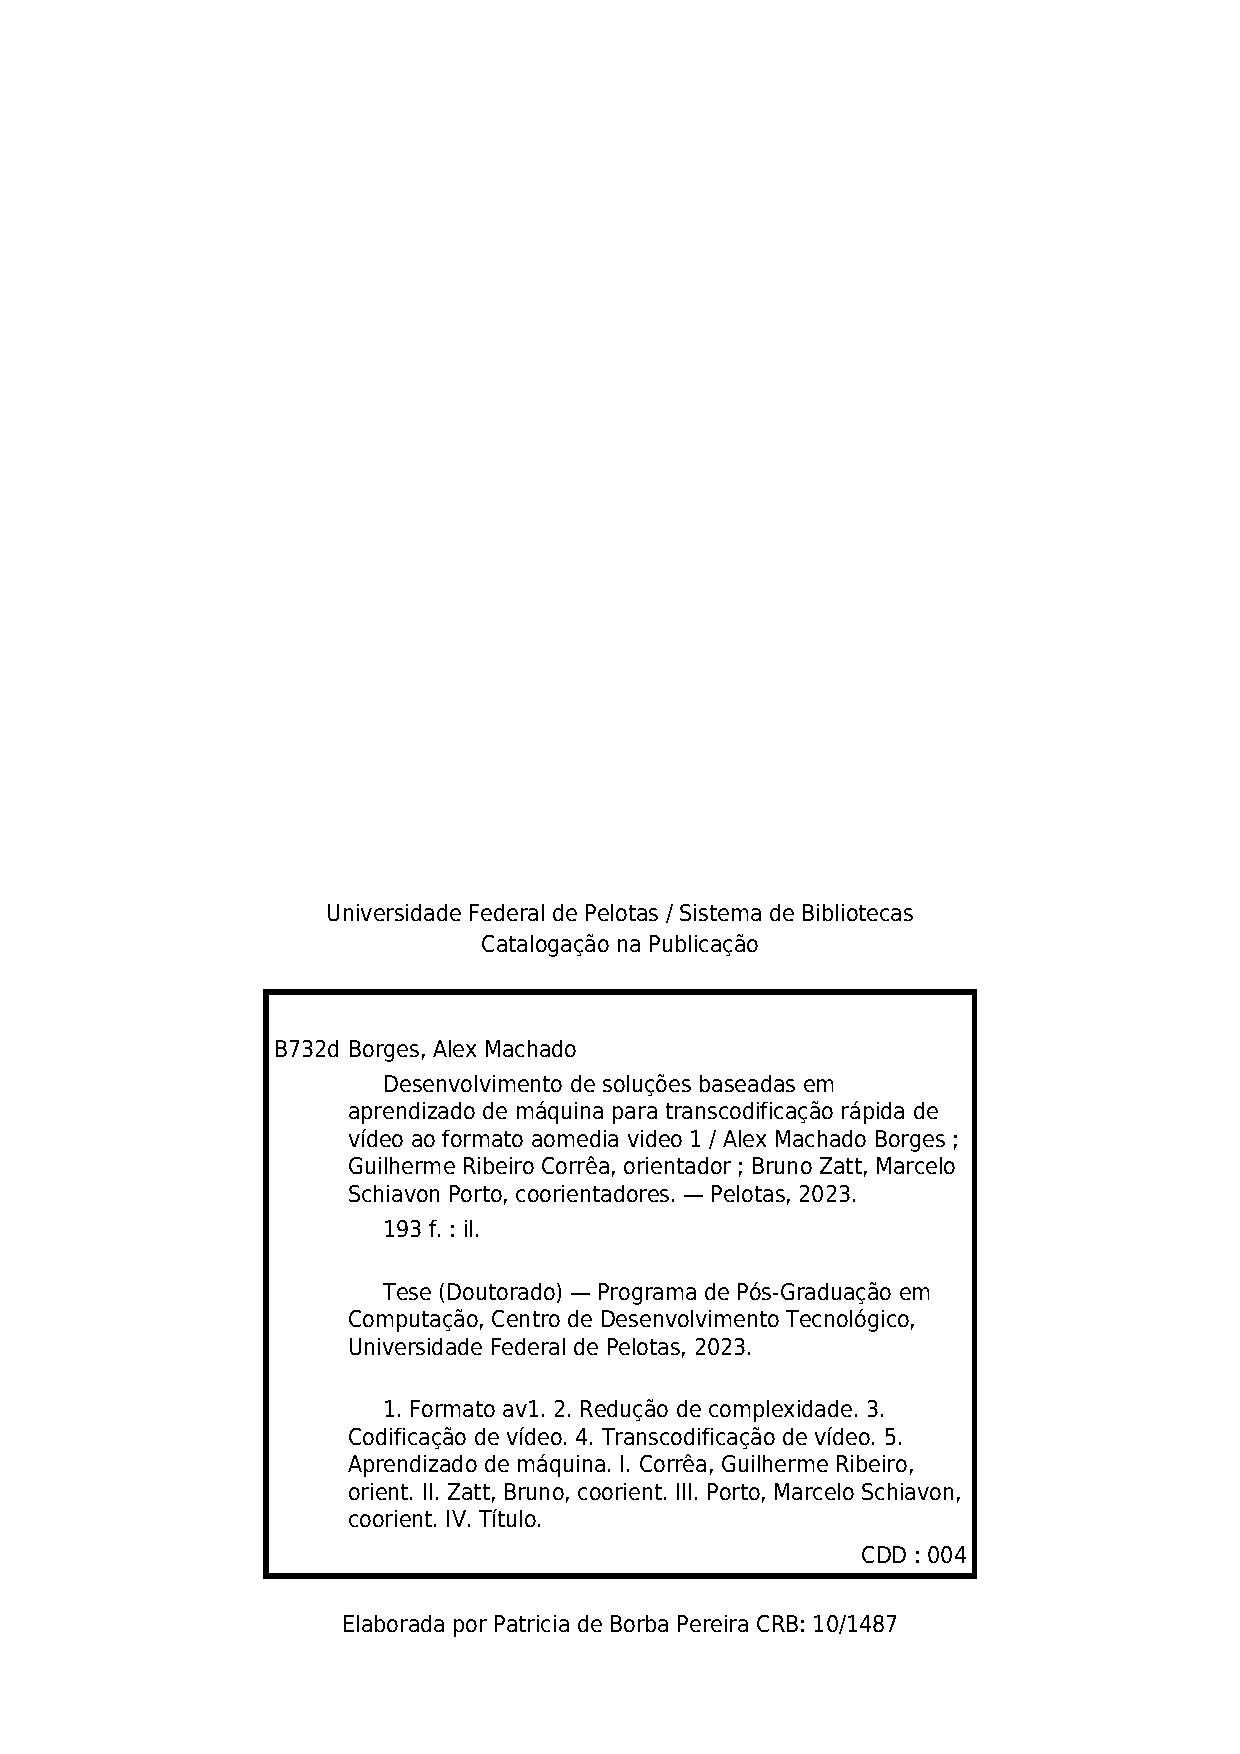
\includepdf[fitpaper=true, pages=-]{FIGURES/ficha_catalografica.pdf}
%\begin{figure}
%    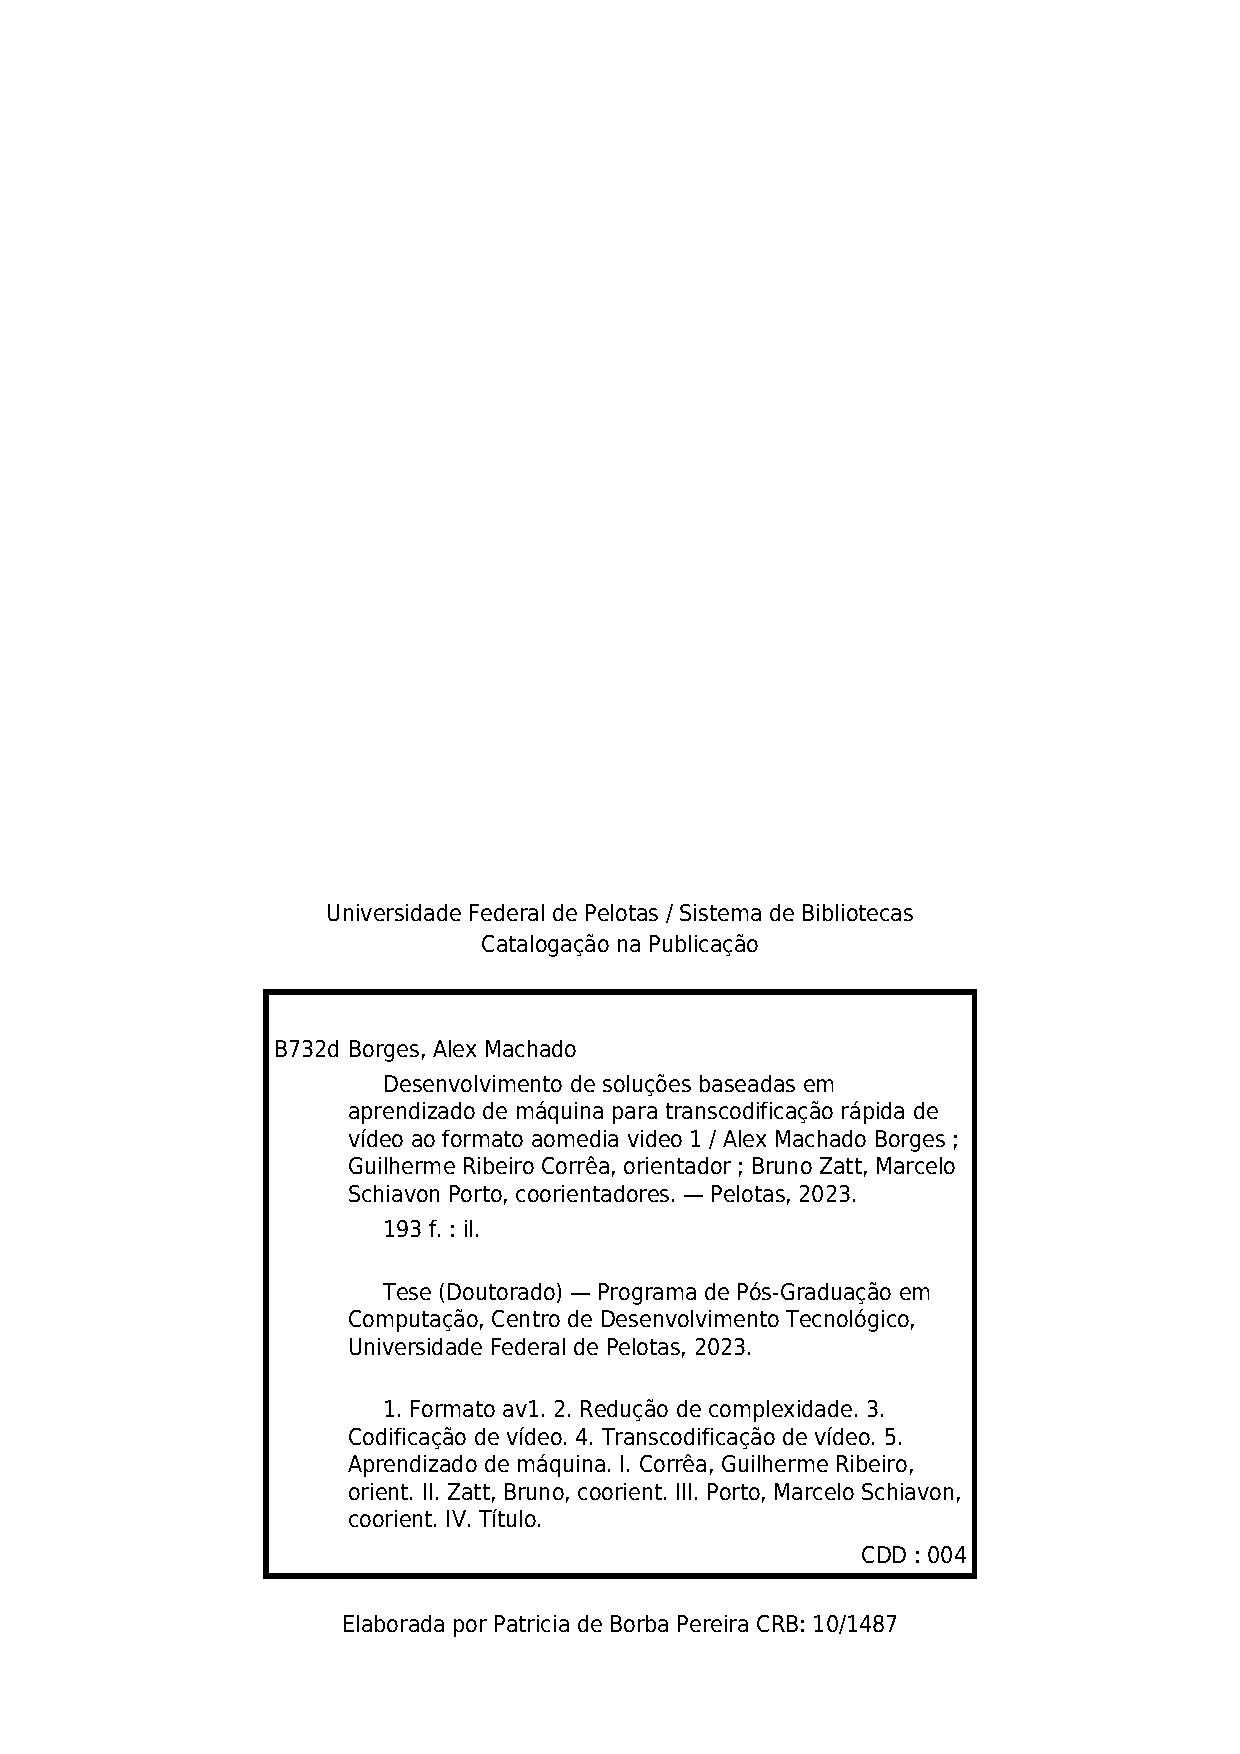
\includegraphics{FIGURES/ficha_catalografica.pdf}
%\end{figure}
%\fichacatalografica

%Composição da Banca Examinadora
\begin{aprovacao}{15 de março de 2023} %data da banca por extenso
\noindent Prof. Dr. Guilherme Ribeiro Corrêa (orientador)\\
Doutor em Engenharia Electrotécnica e de Computadores pela Universidade de Coimbra, Portugal.\\[1cm]

\noindent Prof. Dr. Eduardo Peixoto Fernandes da Silva\\
Doutor em Engenharia Eletrônica pela Queen Mary University of London, Reino Unido.\\[1cm]

\noindent Prof. Dr. Mateus Grellert da Silva\\
Doutor em Computação pela Universidade Federal do Rio Grande do Sul.\\[1cm]

\noindent Prof. Dr. Luciano Volcan Agostini\\
Doutor em Computação pela Universidade Federal do Rio Grande do Sul.
\end{aprovacao}

%Opcional
%\begin{dedicatoria}
%  Dedico\ldots 
%\end{dedicatoria}

%Opcional
\begin{agradecimentos}
Este texto e todo o trabalho oculto atrás das palavras aqui escritas só foram possíveis graças a algumas pessoas que estiveram ao meu lado ao longo dos últimos anos. Neste fim de uma era cheia de estudos e fortes labutas, torna-se impossível agradecer a todos. Principalmente tendo em vista a trágica fase da educação e ciência que o nosso país tem vivenciado. No entanto, algumas pessoas precisam ser citadas:
  
Em primeiro lugar, ao amor de minha vida, \textbf{Janaína Araujo}. Obrigado por ser o meu porto seguro, mesmo nas horas mais sombrias. Sem ti, desde os mínimos detalhes, nada nesta vida faria sentido.
  
Em segundo lugar, aos meus pais, \textbf{Ceni Alaniz e Paulo Borges}, que, desde o começo dessa minha jornada na academia, tornaram tudo possível. Sem vocês, eu nada seria.

Em terceiro lugar, ao meu orientador \textbf{Guilherme Corrêa}, pela paciência e o estímulo. Sei bem que não sou o ideal de orientando: teimoso, confuso e insistente. Obrigado pelos aprendizados e oportunidades. Espero, sinceramente, que este não seja o fim desta amizade. A boa notícia é que se tu conseguiste sobreviver à minha orientação, irás sobreviver a tudo! haha
  
Em quarto lugar, aos \textbf{meus colegas} mais próximos: Bianca da Silveira, Isis Bender, Marcel Moscarelli, Rafael Ferreira, Renira Soares e Roberta Palau. As nossas intensas trocas de ideias, principalmente no começo do doutorado, serviram muito como uma quase via dupla de co-orientação. Acredito que muitos dos nossos trabalhos evoluíram graças aos nossos papos. Obrigado por dividirem comigo essa longa trilha que é ser pesquisador no Brasil.
  
Em quinto lugar, à minha orientanda \textbf{Caroline Camargo}, que me auxiliou na habilidade de ensinar e me encantou na arte de aprender com os mais novos. Foi com essa nossa relação que aprendi a cobrar e ser cobrado. Meu muito obrigado. Continue sendo essa pesquisadora maravilhosa.

Em sexto lugar, um agradecimento especial para mim mesmo e todas as \textbf{vozes da minha cabeça}. Nada teria saído do papel sem os longos e intensos debates que tivemos.

Em sétimo lugar, à \textbf{Aline Duvoisin}, um muitíssimo obrigado por ter sido a minha primeira leitora da tese. Tuas observações e correções auxiliaram imensamente para tornar este texto compreensível para grande parte das pessoas fora da área da Computação. 

Em oitavo lugar, à \textbf{Patrícia Borba}, pois há dez anos fostes tu quem primeiro me direcionou ao universo acadêmico de pesquisas. Só então eu comecei a descobrir o prazer da área, apesar de todos os perrengues. Meu eterno muitíssimo obrigado!
  
Também devo meu muito obrigado a todos os que colaboraram com a minha caminhada até este momento: amigos antigos e novos, colegas de várias jornadas, professores e família. As coisas só fazem sentido quando olhamos para trás e apreciamos a jornada. Inenarrável é o prazer de fazer parte da vida de vocês! 

Por fim, não posso deixar de mencionar o clássico agradecimento que tem me acompanhado na última década de vida como pesquisador. Mesmo considerando a gestão que acompanhou o meu caminho neste doutorado, sem esse especial agradecimento provavelmente não haveria tanta ciência de ponta sendo feita neste país. Por isso, pela última vez como aluno, digo: \texttt{This study was financed in part by the \textit{Coordenação de Aperfeiçoamento de Pessoal de Nível Superior} – Brasil (CAPES) – Finance Code 001, Foundation for Research Support of the State of Rio Grande do Sul (FAPERGS), and National Council for Scientific and Technological Development (CNPq)}.

\end{agradecimentos}


%Opcional
\begin{epigrafe}
Traidor da Constituição é traidor da Pátria. Conhecemos o caminho maldito. Rasgar a Constituição, trancar as portas do Parlamento, garrotear a liberdade, mandar os patriotas para a cadeia, o exílio e o cemitério. \\
Quando, após tantos anos de lutas e sacrifícios, promulgamos o Estatuto do Homem, da Liberdade e da Democracia, bradamos por imposição de sua honra. \\
Temos ódio à ditadura. \\
\\
ÓDIO E NOJO. \\
\\
{\sc --- Ulisses Guimarães\\
(5 de outubro de 1988)}
\end{epigrafe}

%Resumo em Portugues (no maximo 500 palavras)
\begin{abstract}
Codificadores de vídeo são ferramentas importantíssimas atualmente para a viabilização de aplicações comuns no nosso cotidiano, seja em aplicativos dedicados à transmissão de vídeo para entretenimento, como YouTube e Netflix, seja em redes sociais, como Instagram ou TikTok, ou ainda para comunicação privada, como em chamadas de vídeo. Não à toa, mesmo com uso de codificadores de vídeo eficientes, conteúdos de vídeo representam uma parcela considerável do tráfego de dados mundial pela internet. Por este motivo, esta é uma área de relevância ímpar na comunidade científica e a definição de novos padrões e formatos de compressão de vídeo cada vez mais eficientes tem sido uma constante. Considerando o grande número de formatos e padrões de codificação, a modificação de arquivos de vídeo para diversos fins é uma prática comum, seja para prover compatibilidade entre dispositivos ou ainda para adequar um vídeo codificado a situações adversas, como adaptação de taxa de bits e resolução. Essa modificação é chamada de transcodificação de vídeo e possui diversas aplicações. Uma das aplicações, denominada transcodificação heterogênea, tipicamente envolve a atualização de vídeos codificados em um formato mais antigo para outro mais recente e com maior eficiência de compressão. Contudo, essa tarefa exige um significativo esforço computacional, pois envolve uma decodificação e uma nova codificação em sequência. Por isso, parte da comunidade científica atuante na área de codificação de vídeo vem buscando soluções para acelerar o processo de transcodificação de vídeo. Esta tese está centrada neste objetivo. A tese apresenta inicialmente o estado da arte em transcodificação de vídeo, suas aplicações e técnicas. Nesta tese, são apresentadas sete propostas de transcodificadores rápidos para o formato AOMedia Video 1 (AV1), partindo de outros formatos largamente utilizados pela indústria de \textit{streaming} de vídeo. Dentre as propostas realizadas, destacam-se aquelas que empregam modelos preditivos treinados por algoritmos de aprendizado de máquina para acelerar as decisões de particionamento do codificador. De forma a possibilitar o desenvolvimento ágil de transcodificadores rápidos, esta tese também propõe um \textit{pipeline} de processamento, que permite, dentre outras coisas, a automatização do treinamento de modelos preditivos e o escalonamento de experimentos para testá-los. Como prova de conceito a essa proposta metodológica, cinco transcodificadores de vídeo rápidos foram desenvolvidos com o \textit{pipeline}, todos eles empregando modelos preditivos do tipo árvore de decisão. Os resultados obtidos indicam que é possível acelerar o processo de transcodificação para o formato AV1 entre 12\% e 55\%, com perdas em eficiência de codificação que variam entre 1,6\% e 12,8\%, dependendo do formato de origem.
\end{abstract}

%Resumo em Inglês (no maximo 500 palavras)
\begin{englishabstract}{Development of Machine Learning-Based Solutions for Fast Video Transcoding to the Format AOMedia Video 1}
Video encoders are currently very important tools for enabling common applications in our daily lives, whether in applications dedicated to video transmission for entertainment, such as YouTube and Netflix, or in social networks, such as Instagram or TikTok, or even for private communication, such as on video calls. Even with the use of efficient video encoders, video content represents a considerable portion of the world's data traffic over the Internet. For this reason, this is an area of unique relevance in the scientific community and the definition of new standards and video compression formats has been a constant. Considering the large number of video formats and standards, modifying encoded video files for different purposes is a common practice, whether to provide compatibility between devices or even to adapt a coded video to different situations, such as bit rate adaptation and resolution change. This modification is called video transcoding and has several applications. One of the applications, called heterogeneous transcoding, tipically involves updating videos encoded in an older format to a more recent one with greater compression efficiency. However, this task requires a significant computational effort, as it involves decoding and re-encoding the video in sequence. Therefore, part of the scientific community active in the video coding field has been looking for solutions to speed up the video transcoding process. This thesis is focused on this goal. The thesis initially presents the state of the art in video transcoding, its applications and techniques. In this thesis, seven fast transcoders are proposed for the AOMedia Video 1 (AV1) format, based on other formats widely used by the video \textit{streaming} industry. Among the proposals, those that employ predictive models trained by machine learning algorithms to accelerate the encoder partitioning decisions stand out. In order to enable the agile development of fast transcoders, this thesis also proposes a processing pipeline, which allows, among other things, the automation of training predictive models and the scheduling of experiments to test them. As a proof of concept for this methodological proposal, five fast video transcoders were developed with the pipeline, all of them employing decision tree models. The obtained results indicate that it is possible to accelerate the transcoding process for the AV1 format between 12\% and 55\%, with losses in coding efficiency that vary between 0.96\% and 12.85\%, depending on the source format.
\end{englishabstract}

%Lista de Figuras
\listoffigures

%Lista de Tabelas
\listoftables

%lista de abreviaturas e siglas
\begin{listofabbrv}{BD-rate}%coloque aqui a maior sigla para ajustar a distância
        \item[ACM] Association for Computing Machinery
        \item[AI] inteligência artificial
        \item[AV1] AOMedia Video 1
        \item[AVC] Advanced Video Coding
        \item[AVS] Audio Video Standard
        \item[AUC] Area Under the Curve ROC
        \item[BD-rate] Bj{\o}ntegaard Delta-rate
        \item[CART] Classification and Regression Trees
        \item[CNN] Convolutional Neural Network
        \item[CQ] nível de Constrained Quality
        \item[CTU] Coding Tree Units
        \item[CU] Coding Unit
        \item[DOI] Digital Object Identifier
        \item[HD720] Vídeos de Alta Resolução, com 1280$\times$720 pixels
        \item[HD1080] Vídeos de Alta Resolução, com 1920$\times$1080 pixels
        \item[HDR] High Dynamic Range
        \item[HEVC] High Efficiency Video Coding
        \item[HRSCV] \textit{Halving Random Search with Cross Validation}
        \item[LDF] Linear Discriminant Functions
        \item[LSTM] Long Short-Term Memory
        \item[ML] Aprendizado de Máquina
        \item[MLR] Multiple Linear Regression
        \item[MPEG] Moving Picture Experts Group
        \item[PSNR] Peak Signal-to-Noise Ratio
        \item[PU] Prediction Unit
        \item[QP] nível de Quantization Parameter level
        \item[rd-cost] custo taxa-distorção
        \item[RDO] Rate-Distortion Optimization 
        \item[RGS] Random Grid Search
        \item[ROC] Receiver Operating Characteristics
        \item[SB] Superbloco
        \item[SCC] Screen Content Coding
        \item[SVM] Support Vector Machine
        \item[TS] Redução de Tempo da Transcodificação
        \item[UHD4K] Vídeos de Ultra-Alta Resolução, com 4196$\times$2160 pixels
        \item[VMAF] Video Multi-Method Assessment Fusion
        \item[VVC] Versatile Video Coding
\end{listofabbrv}

%Sumario
\tableofcontents

\chapter{Introdução}
\label{cap:1}

A tecnologia de captura e reprodução de vídeos foi inventada pelos irmãos Auguste Lumière e Louis Lumière, no final do ano de 1895 \cite{bib:lumiere}. No entanto, somente na década de 1970 foram desenvolvidas tecnologias de vídeos digitais \cite{bib:videocodechistory} e elas demandavam um elevado número de bits para armazenar o conteúdo capturado, o que trouxe consigo uma necessidade de redução deste volume de bits e, consequentemente,  do espaço de armazenamento necessário para armazená-los. Ou seja, os vídeos digitais exigiram a criação de compressores especializados em vídeo digitais.

Desde o lançamento do primeiro padrão de codificação de vídeo na década de 1980 (H.120 \cite{bib:h120}), o volume de conteúdo em vídeo tem crescido na sociedade, principalmente após a popularização de dispositivos móveis com capacidade de captura e reprodução de vídeos, em associação a melhorias na largura de banda da rede de internet, sendo que, atualmente, o conteúdo em vídeo é um dos tipos de mídia mais consumidos ao redor do mundo. Reuniões e aulas on-line, filmes e séries disponíveis em serviços de \textit{streaming}, jogos on-line e muitos outros são exemplos notórios da presença de conteúdo em vídeo no nosso dia a dia. Segundo \cite{bib:statista_2021}, no primeiro trimestre de 2019, 85\% de todos os dispositivos móveis do mundo acessaram algum conteúdo de vídeo on-line. Além disso, um relatório publicado em 2018 \cite{bib:statistaVideoTraffic} indicou que o conteúdo em vídeo foi responsável por 60\% de todo o tráfego de dados da internet. Estes autores preveem um crescimento desse tipo de conteúdo nos próximos anos, principalmente devido à popularização de vídeos em \textit{Ultra-High Definition} 4K (UHD4K), conforme apontado por \cite{bib:cisco_2020} e \cite{bib:bitmovin_report_2021}.

De fato, a pandemia de COVID-19 (SARS-CoV2 \cite{bib:covid19}) agravou esse cenário de crescimento, pois houve uma intensificação de campanhas de trabalhos remotos e aulas a distância, juntamente com o surgimento de novas distribuidoras de conteúdo digital, como Apple+, Disney+, HBO Max e muitas outras, como afirma \citet{bib:bitmovin_report_2020}, ocasionando um crescimento do consumo de conteúdo em vídeo digital de 30\% \cite{bib:ramirez_2020, bib:clapp_2021} a 300\% \cite{bib:bottger_2020} em todo o mundo. E, de acordo com \cite{bib:verizon_2021}, o tráfego de dados relacionados a jogos on-line cresceu 71\% nos primeiros meses da pandemia.

Desde a publicação do H.120 \cite{bib:h120}, em 1984, muitos outros formatos e padrões de codificação de vídeo foram publicados nas últimas quatro décadas, como mostra a Figura \ref{fig:1}. Alguns desses codificadores foram definidos por organizações mundiais como a Organização Internacional para Padronização (do inglês, \textit{International Organization for Standardization}, ISO), a Comissão Eletrotécnica Internacional (do inglês, \textit{International Electrotechnical Commission}, IEC) e a União Internacional de Telecomunicações (do inglês, \textit{International Telecommunication Union}, ITU). Outros formatos foram definidos por empresas e consórcios do setor, como o grupo \textit{Alliance for Open Media} (AOMedia), e, por não terem sido definidos por órgãos mundialmente reconhecidos, não podem receber a nomenclatura de padrão. Dentre os padrões de codificação, destacam-se os mais famosos: o H.262/MPEG-2 \cite{bib:mpeg2} e o H.264/AVC \cite{bib:h264overview2}. Enquanto o H.262/MPEG-2 foi amplamente utilizado para codificar vídeos para mídia de DVD, o H.264/AVC tem sido mais usado em conteúdos para a internet, contribuindo para a popularização do consumo de vídeos on-line. Inclusive, o padrão H.264/AVC é utilizado no Sistema Brasileiro de Televisão Digital \cite{bib:dissertacao_rodrigues_2008}. A Figura \ref{fig:1} mostra que a tecnologia de codificação de vídeo continuou evoluindo e, apesar do H.264/AVC ainda estar presente em 78\% do mercado mundial de vídeos, conforme \cite{bib:bitmovin_report_2022}, há quatro novos codificadores de vídeo que representam a tecnologia de ponta da atualidade: o \textit{AOMedia Video} 1 (AV1) \cite{bib:av1_overview_2021}, o \textit{Versatile Video Coding} (H.266/VVC) \cite{bib:vvc}, o \textit{MPEG-5 Essential Video Coding} (MPEG-5 EVC) \cite{bib:evc} e o \textit{Audio Video Standard Third Generation} (AVS3) \cite{bib:avs3}. Ainda na Figura \ref{fig:1} é possível observar diversos formatos e padrões de codificação de vídeo que foram publicados ao longo dos anos, com vários deles estando disponíveis para uso por parte da indústria e da população.

%O comando abaixo cria um texto com bordas redondas contendo o ano
\newcommand{\textoano}[3]{ \fill[black] (#1, #2) node [yearblock] {#3}; }
%O comando abaixo cria um texto simples que está ligado à linha principal através de uma linha vertical
\newcommand{\textoref}[3]{ 
\fill[black] (#1, #2) circle(0.1cm);
    \draw (#1, #2) -- (#1, #2 - 0.7); 
    \node at (#1, #2 - 1) [nameblock] {#3};
}
%O comando abaixo é igual ao de cima, mas a distância da linha e do texto é 0.3cm menor
\newcommand{\textorefup}[3]{ 
\fill[black] (#1, #2) circle(0.1cm);
    \draw (#1, #2) -- (#1, #2 - 0.5); 
    \node at (#1, #2 - 0.7) [nameblock] {#3};
}

%o comando abaixo adiciona reticências no final do desenho
\newcommand{\tobecontinue}[2]{ 
\fill[black] (#1 + 0.1, #2) circle(0.05cm);
\fill[black] (#1 + 0.3, #2) circle(0.05cm);
\fill[black] (#1 + 0.5, #2) circle(0.05cm);
}

%DISTANCIA ENTRE UM NODO E OUTRO = 0.8
%ALTURA ENTRE AS LINHAS: 2.5

\begin{figure}[!t]
\centering
\scriptsize
\begin{tikzpicture}
\draw (0,10) -- (14.3,10) -- (14.3, 7.5) -- (-0.8, 7.5) -- (-0.8, 5) -- (14.3, 5) -- (14.3, 2.5) -- (-0.8, 2.5) -- (-0.8,0) -- (13.5,0);

\textoano{0}{10}{1984}

    \textoref{0.8}{10}{H.120}% \cite{bib:5to9google}}

\textoano{1.6}{10}{1985}
\textoano{3.2}{10}{1986}
\textoano{4.8}{10}{1987}
\textoano{6.4}{10}{1988}

    \textoref{7.2}{10}{H.261}% \cite{bib:h261}}

\textoano{8}{10}{1989}
\textoano{9.6}{10}{1990}

    \textorefup{10.4}{10}{TrueMotion S}% \cite{bib:TrueMotion}}

\textoano{11.2}{10}{1991}

    \textoref{12}{10}{Cinepak}% \cite{bib:cinepak}}

\textoano{12.8}{10}{1992}
\textoano{13.6}{7.5}{1993}

    \textorefup{12.8}{7.5}{Indeo Video 3}% \cite{bib:indeo3}}

\textoano{12}{7.5}{1994}
\textoano{10.4}{7.5}{1995}

    \textoref{9.6}{7.5}{H.262/MPEG-2}% \cite{bib:mpeg2}}
    \textorefup{8.8}{7.5}{DV}% \cite{bib:dv_format}}

\textoano{8}{7.5}{1996}

    \textorefup{7.2}{7.5}{H.263}% \cite{bib:h263}}
    \textoref{6.4}{7.5}{TrueMotion RT}% \cite{bib:TrueMotion}}

\textoano{5.6}{7.5}{1997}

    \textorefup{4.8}{7.5}{MJPEG}% \cite{bib:mjpeg}}
    \textoref{4}{7.5}{TrueMotion 2}% \cite{bib:TrueMotion}}

\textoano{3.2}{7.5}{1998}

    \textorefup{2.4}{7.5}{Sorenson Video}% \cite{bib:sorenson}}

\textoano{1.6}{7.5}{1999}

    \textoref{0.8}{7.5}{WMV-7}% \cite{bib:wmv9}}

\textoano{0}{5}{2000}

    \textorefup{0.8}{5}{VP3}% \cite{bib:vp3}}
    \textoref{1.6}{5}{Indeo Video 5}% \cite{bib:indeo5}}

\textoano{2.4}{5}{2001}

    \textorefup{3.2}{5}{VP4}% \cite{bib:vp4}}
    \textoref{4}{5}{Sorenson Video 3}% \cite{bib:sorenson3}}
    

\textoano{4.8}{5}{2002}

    \textorefup{5.6}{5}{VP5}% \cite{bib:vp5}}

\textoano{6.4}{5}{2003}

    \textoref{7.2}{5}{H.264/AVC}% \cite{bib:h264overview2}}
    \textorefup{8}{5}{HDV}% \cite{bib:hdv_format}}
    \textoref{8.8}{5}{VP6}% \cite{bib:vp6}}
    \textorefup{9.6}{5}{WMV-9}% \cite{bib:wmv9}}

\textoano{10.4}{5}{2004}

    \textoref{11.2}{5}{Theora}% \cite{bib:theora}}

\textoano{12}{5}{2005}

    \textoref{12.8}{5}{AVS}% \cite{bib:AVS}}
    \textorefup{13.6}{5}{VP7}% \cite{bib:vp7}}

\textoano{13.6}{2.5}{2006}

    \textoref{12.8}{2.5}{VC-1}% \cite{bib:vc-1}}

\textoano{12}{2.5}{2007}
\textoano{10.4}{2.5}{2008}

    \textoref{9.6}{2.5}{VP8}% \cite{bib:vp8}}

\textoano{8.8}{2.5}{2009}

    \textoref{8}{2.5}{VC-2}% \cite{bib:vc-2}}

\textoano{7.2}{2.5}{2010}
\textoano{5.6}{2.5}{2011}
\textoano{4}{2.5}{2012}

    \textoref{3.2}{2.5}{AVS+}% \cite{bib:avs_plus}}
    \textorefup{2.4}{2.5}{VP9}% \cite{bib:vp9overview}}

\textoano{1.6}{2.5}{2013}

    \textorefup{0.8}{2.5}{Daala}% \cite{bib:daala}}
    \textoref{0}{2.5}{H.265/HEVC}% \cite{bib:hevc}}

\textoano{0}{0}{2014}
\textoano{1.6}{0}{2015}

    \textorefup{2.4}{0}{AVS2}% \cite{bib:avs2}}
    \textoref{3.2}{0}{Thor}% \cite{bib:thor}}

\textoano{4}{0}{2016}
\textoano{5.6}{0}{2017}
\textoano{7.2}{0}{2018}

    \textoref{8}{0}{AV1}% \cite{bib:av1_overview_2021}}

\textoano{8.8}{0}{2019}
\textoano{10.4}{0}{2020}

    \textorefup{11.2}{0}{H.266/VVC}% \cite{bib:vvc}}
    \textoref{12}{0}{MPEG-5 EVC}% \cite{bib:evc}}
    \textorefup{12.8}{0}{AVS3}% \cite{bib:avs3}}

\tobecontinue{14}{0}

\end{tikzpicture}
\caption{Alguns formatos de codificação de vídeo publicados nas últimas décadas. Fonte: Elaborada pelo autor.}
\label{fig:1}
\end{figure}
 

No relatório publicado por \citet{bib:bitmovin_report_2021} em 2021, onde foram questionados representantes de diversas empresas atuantes na indústria de \textit{streaming} acerca da distribuição de uso dos codificadores de vídeo, foi possível identificar os principais formatos de codificação utilizados pela indústria. Nesta pesquisa, evidenciou-se que em uma mesma empresa pode utilizar mais de um codificador de vídeo ao mesmo tempo. Logo nenhuma soma de percentuais a seguir irá retornar 100\%. Os codificadores de vídeos mais usados em 2021, além do H.264/AVC \cite{bib:h264overview2} (78\%), foram: o H.265/HEVC \cite{bib:hevc} (49\%), o H.262/MPEG-2 \cite{bib:mpeg2} (31\%), o VP9 \cite{bib:vp9overview} (19\%), o VP8 \cite{bib:vp8} (16\%) e o AV1 \cite{bib:av1_overview_2021} (15\%). Os mesmos autores, em 2022, atualizaram o relatório \cite{bib:bitmovin_report_2022}, apontando que os cinco formatos mais utilizados pela indústria de \textit{streaming} são H.264/AVC (78\%), H.265/HEVC (40\%), H.266/VVC (19\%), VP8 (19\%) e AV1 (18\%). O estudo ainda indicou que os formatos H.265/HEVC e AV1 são os mais cotados para crescimento em 2023, com expectativa de expansão de uso em 43\% e 34\%, respectivamente. No entanto, é importante notar que os estudos não consideraram os formatos AVS1 \cite{bib:AVS}, AVS2 \cite{bib:avs2} e AVS3 \cite{bib:avs3}, amplamente utilizados na China \cite{bib:china_codecs}.

A maioria desses codificadores é capaz de atingir taxas de compressão acima de 99\%, o que é essencial para possibilitar a ampla implantação de sistemas multimídia e transmissão de vídeo pela internet. No entanto, além da taxa de compressão, diversas outras variáveis podem influenciar na decisão de qual codificador escolher, como o nível da qualidade de imagem, o tempo de processamento da codificação/decodificação, o consumo de energia requerido para utilizar o codificador e até mesmo licenciamento de propriedade intelectual. Assim, considerando a grande pluralidade de codificadores de vídeo disponíveis atualmente, a conversão entre formatos é necessária para permitir a compatibilidade entre eles.

Uma prática comum aplicada pela indústria de multimídia para obter essa compatibilidade é a utilização de transcodificadores de vídeo. Há muitas razões para alterar o formato de vídeo compactado, como converter arquivos de vídeo antigos para formatos novos e mais eficientes, fornecer compatibilidade entre gerações de dispositivos antigos com vídeos gerados sob novos formatos, adaptar a resolução de vídeo à exibição disponível ou a taxa de bits do vídeo para a largura de banda de internet disponível do usuário e muitos outros. Um exemplo do uso de transcodificador pode ser observado por dois dos principais serviços de \textit{streaming} de vídeo do mundo, o YouTube e a Netflix, que viabilizam a boa experiência ao usuário ao manter várias versões de um mesmo vídeo com diferentes taxas de bits e de resoluções em seus servidores. A criação dessas versões dos vídeos é feita através de um \textit{pipeline} de transcodificação \cite{bib:netflix_pipeline}.

Diferentes estratégias de transcodificação de vídeo podem ser encontradas na literatura, almejando prover a melhor experiência do usuário (do inglês, \textit{Quality of Experience}, QoE) e/ou a melhor qualidade de serviço (do inglês, \textit{Quality of Service}, QoS), especialmente quando há o envolvimento de transmissão de vídeo pela internet. Muitas dessas soluções visam acelerar a transcodificação, já que é um processo lento devido à alta complexidade dos codificadores de vídeo, principalmente os mais recentes, tal como demonstram \citet{bib:hevc_complexity} e \citet{bib:vvc_complexity}, assim como outros trabalhos recentes da literatura. Diferentes estratégias podem ser empregadas para reduzir essa complexidade, a depender do objetivo geral, tais como: reutilizar diretamente as decisões herdadas do formato bitstream anterior, por exemplo em \citet{bib:wang_2012} e \citet{bib:nguyen_2015}; treinar modelos de aprendizado de máquina para prever os melhores modos de codificação para o novo formato, como em \citet{bib:peixoto_2014}; ou mesmo predizer tamanhos de blocos a serem utilizadas em uma transcodificação de redimensionamento do tamanho da imagem, como em \citet{bib:lin_2016}. Embora muitas propostas tenham sido publicadas na literatura científica, em especial na última década, ainda há brechas a serem estudadas, principalmente quando se trata de novos formatos com maior poder de compressão de dados e elevada complexidade de execução.

Portanto, nesta tese de doutorado, apresentamos um levantamento bibliográfico acerca dos artigos de transcodificação de vídeo publicados entre os anos de 2011 e 2022. Com isso, é possível obter uma visão geral do estado da arte sobre transcodificação de vídeo, permitindo compreender o que vem sendo explorado nas pesquisas e identificar tópicos pouco abordados e desafios ainda em aberto na literatura vigente. Após essa abordagem, desenvolvemos propostas de transcodificação rápida de vídeo ao formato de vídeo \textit{AOMedia Video} 1 (AV1), a partir dos formatos VP8, VP9, H.264/AVC, H.265/HEVC e H.266/HEVC, cinco dos formatos de codificação de vídeo mais utilizados pela indústria de \textit{streaming} de vídeo, conforme já demonstrado por \citet{bib:bitmovin_report_2021} e \citet{bib:bitmovin_report_2022}.

Esta tese tem, como \textbf{objetivo geral}, o desenvolvimento de um \textit{pipeline} de processamento que possibilite a definição de transcodificadores rápidos de vídeo para o formato \textit{AOMedia Video} 1 (AV1) a partir de diversos outros formatos. Assim, a \textbf{hipótese} que norteou o desenvolvimento desta investigação foi a seguinte: \textit{a transcodificação de vídeo para o formato AV1 pode ser acelerada, com baixo impacto na eficiência de codificação, por meio do uso de uma metodologia comum para treinamento de modelos preditivos baseados em aprendizado de máquina, buscando inferir decisões na codificação a partir de dados extraídos tanto do bitstream original como do próprio processo de re-codificação}.

Ou seja, verificamos a possibilidade de que uma mesma metodologia de transcodificação de vídeo possa ser utilizada para acelerar diferentes transcodificadores e, mesmo assim, obter resultados de aceleração e impacto na eficiência de codificação similares aos demais trabalhos observados na literatura, que empregam metodologias variadas.

As principais contribuições científicas, tecnológicas e bibliográficas desta tese para a área de codificação de vídeo são:

\begin{itemize}
    \item Uma revisão bibliográfica da literatura da última década sobre transcodificação rápida de vídeo, possibilitando compreender as áreas de interesse e os resultados médios esperados pelos trabalhos de transcodificação rápida;

    \item Uma análise do processo de particionamento de blocos do software de referência do formato AV1, possibilitando compreender a complexidade das decisões tomadas pelo software \textit{libaom} e o impacto das decisões na eficiência de codificação;

    \item Dois transcodificadores rápidos de H.265/HEVC para AV1: o primeiro baseado em heurísticas \cite{bib:borges2_2021} e o segundo baseado em modelos preditivos gerados por algoritmos de aprendizado de máquina;

    \item Dois transcodificadores rápidos de VP9 para AV1: o primeiro baseado em heurísticas \cite{bib:borges_2021} e o segundo baseado em modelos preditivos gerados por algoritmos de aprendizado de máquina;

    \item Três transcodificadores rápidos inéditos na literatura científica, VP8-para-AV1, H.264/AVC-para-AV1 e H.266/VVC-para-AV1, todos eles baseados em modelos preditivos gerados por algoritmos de aprendizado de máquina;

    \item Um \textit{pipeline} de processamento automatizado para geração de modelos preditivos gerados por aprendizado de máquina que auxiliam na aceleração de transcodificadores de vídeo.
\end{itemize}

Para expor o trabalho desenvolvido, dividimos esta tese em sete capítulos. O capítulo \ref{cap:2} aborda os conceitos básicos necessários para a compreensão do restante do texto. O capítulo \ref{cap:3} trata da metodologia para revisão sistemática da literatura e dos resultados obtidos nesta etapa. O capítulo \ref{cap:4} descreve a metodologia geral aplicada para desenvolvimento das soluções propostas nesta tese, como sequências de vídeo e softwares utilizados. O capítulo \ref{cap:5} apresenta um estudo sobre a complexidade do codificador de vídeo AV1. O capítulo \ref{cap:6} apresenta duas soluções de transcodificação rápida baseadas em heurísticas e discute os resultados obtidos. O capítulo \ref{cap:7} apresenta o desenvolvimento de transcodificadores rápidos baseados em modelos preditivos gerados por aprendizado de máquina, descreve o \textit{pipeline} de processamento desenvolvido para esse fim e discute os resultados obtidos. Por fim, o capítulo \ref{cap:conclusao} apresenta as conclusões desta tese de doutorado.

\chapter{Conceitos Básicos}
\label{cap:2}

Reproduzir uma sequência de imagens similares para criar uma ilusão de movimento é uma prática existente desde o final do século XIX, tal como consta em \cite{bib:sciam_firstmotion}, publicação científica mais antiga sobre o tema. Cada nova imagem (denominada quadro) é sutilmente diferente da anterior, sendo que esta sutileza cresce à medida que aumenta a velocidade de captação entre essas imagens. Ao compararmos dois quadros próximos, constatamos que a diferença entre eles tende a ser mínima, ainda mais quando se tratam de vídeos com alta taxa de transição de imagem para cada unidade de tempo considerado, normalmente um segundo. 

Em um vídeo digital, cada quadro é composto por partes menores, denominadas pixels. Sendo o pixel o menor elemento de uma imagem digital, este é, por sua vez, o elemento que informa a cor de cada ponto daquela imagem. Os pixels representam valores em um padrão de cores. Normalmente, três valores inteiros, chamados de amostras, são utilizados para representar a intensidade de vermelho, verde e azul, no caso do sistema de cores RGB, ou de luminância, crominância azul e crominância vermelha, no caso do sistema de cores YCbCr \cite{bib:sistema_cores}.

No caso de vídeos armazenados digitalmente, observamos que a maior parte de um vídeo sem compressão conterá dados redundantes. Para possibilitar a redução desses dados, a codificação de vídeos deve ser especializada em identificar e explorar três tipos de redundância, conforme afirma \cite{bib:tese_agostini_2007}. As redundâncias que o codificador de vídeo busca identificar são: 

\begin{enumerate}[a)]
    \item \textbf{Redundância Temporal}: manifesta-se através da existência de dados repetidos entre dois quadros vizinhos;

    \item \textbf{Redundância Espacial}: manifesta-se através da existência de dados repetidos dentro de um mesmo quadro;

    \item \textbf{Redundância Entrópica}: manifesta-se através da distribuição dos símbolos, ou probabilidade de ocorrência de símbolos, em um vídeo.
\end{enumerate}

Apesar de haver diversos codificadores de vídeo desenvolvidos para determinados fins, em geral os formatos e padrões lançados nas últimas duas décadas são classificados como formatos de codificação de vídeo híbrida \cite{bib:richardson_2002}, ou seja, combina diversas técnicas de codificação visando alcançar o melhor resultado possível em termos de eficiência de compressão. Essa codificação híbrida é baseada em blocos, onde cada bloco é composto por um conjunto de pixels, também denominados de amostras. Eles recebem essa classificação por explorarem diversos tipos de redundâncias a fim de atingir altas taxas de compressão \cite{bib:tese_agostini_2007}. Apesar dos formatos possuírem diferenças pontuais, é possível resumir o fluxo de execução de um codificador de vídeo híbrido baseado em blocos conforme a Figura \ref{fig:2}. Todas essas etapas são executadas ou associadas ao nível de bloco e, apesar dos codificadores modernos já serem mais complexos do que o explicado aqui, o resumo dessas etapas segue conforme listado abaixo:

\begin{figure}
    \centering
    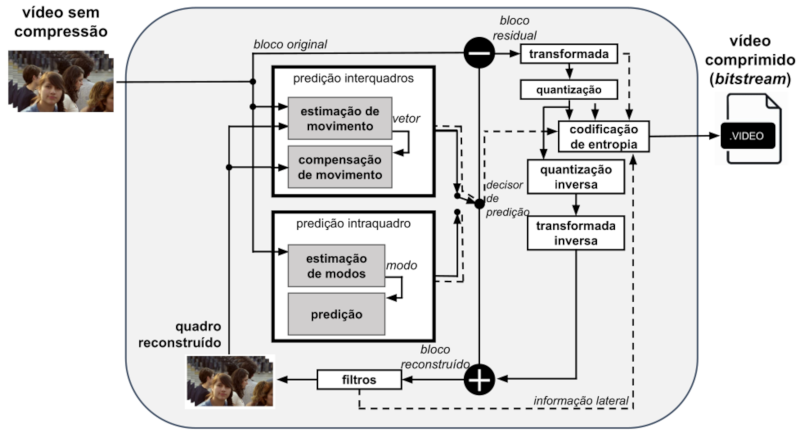
\includegraphics[width=\textwidth]{FIGURES/fig_2.png}
    \caption{Representação em alto nível de um codificador de vídeo híbrido. Fonte: Elaborada pelo autor.}
    \label{fig:2}
\end{figure}


\begin{itemize}
    \item \textbf{Predição Intraquadro}: responsável por predizer os valores das amostras do bloco que se está processando apenas utilizando informações do próprio quadro de origem do bloco, de forma a reduzir a redundância espacial. Para tanto, são usados modos de predição que indicam ao codificador/decodificador em qual direção está a amostra que contém o valor que deve ser copiado. O primeiro quadro de cada vídeo codificado, atualmente, é somente processado por esse tipo de predição, já que não há dependência de dados anteriores para sua funcionalidade. Além disso, esse tipo de quadro exclusivo de predição intraquadro também é utilizado, por exemplo, para sincronização durante transmissões ao vivo;

    \item \textbf{Predição Interquadros}: responsável por reduzir a redundância temporal, é uma predição dependente de quadros vizinhos para ser executada. Seu funcionamento consiste em varrer blocos de amostras do quadro de referência (localizados anteriormente ou posteriormente ao quadro atual) buscando um bloco que seja igual ou similar ao bloco de amostras sob codificação no momento. O resultado dessa predição é um vetor de movimento que aponta o deslocamento que deve ser realizado, a partir da posição do bloco sob codificação, para encontrar o bloco de referência;

    \item \textbf{Transformada}: da subtração do bloco predito com o bloco original, obtém-se um bloco residual. Este bloco é importante pois define diferença entre os blocos original e predito, ou seja, define o erro de predição (seja intraquadro ou interquadros). Entretanto, ele representa informações no domínio espacial, no qual as amostras ainda estão correlacionados entre si, o que leva a um baixo desempenho da codificação de entropia. Para possibilitar uma decorrelação da informação residual e concentrá-la em um pequeno número de coeficientes, os blocos residuais são submetidos a um processo de transformação do domínio de representação, passando-os do domínio espacial para o domínio de frequências;

    \item \textbf{Quantização}: com os dados representados no domínio das frequências e considerando o funcionamento do sistema visual humano, é possível atenuar, ou mesmo eliminar, frequências mais elevadas que pouco contribuem para a formação da imagem pelo olho humano. Esse processo de atenuação/eliminação é feito nesta etapa de codificação, na qual ocorre a aplicação de um parâmetro de quantização sobre os coeficientes transformados, gerando um bloco quantizado. Até esta etapa, ao menos para os formatos publicados nas últimas duas décadas, todos os processos realizados são totalmente reversíveis, no entanto, após a aplicação da quantização, informações são irreversivelmente descartadas e, portanto, perdas na qualidade da imagem são geradas;

    \item \textbf{Codificação de Entropia}: responsável pela compressão propriamente dita. A codificação de entropia processa os dados transformados e quantizados, assim como as informações laterais (modos decididos, tamanhos de blocos, etc.). Todos os estágios de codificação servem para tornar este estágio mais eficiente, pois quanto menores são os resíduos e, consequentemente, mais concentrados são os coeficientes transformados e quantizados, maior é a taxa de compressão obtida pela codificação de entropia. Ao final desta etapa, é gerado um \textit{bitstream} compatível com o formato de vídeo utilizado durante a codificação;

    \item \textbf{Filtros}: responsável por reduzir, ou mesmo eliminar, artefatos de compressão causados pela etapa de quantização. Há diversos artefatos de compressão, apresentados em \citet{bib:quantization_artifacts}, como o efeito de bloco, de borramento, entre outros. A aplicação desta etapa de codificação implica na suavização das diferenças entre o vídeo codificado com o vídeo original.

\end{itemize}

Além desses seis estágios de codificação, dentro do próprio codificador inclui-se parte do decodificador, com a quantização inversa e a transformada inversa, com o objetivo de reconstruir o quadro a fim de ser utilizado como referência pelos estágios de predição. Isso serve para garantir que as referências de predições sejam as mesmas no codificador e no decodificador. Apesar de os seis estágios de codificação de vídeo apresentados acima serem similares entre os codificadores de vídeo da atualidade, eles se diferem quanto à forma de executar as operações ou quanto às variações de decisões disponíveis para serem escolhidas. Por exemplo, enquanto o codificador H.264/AVC possui nove modos diferentes de predição intraquadro, o H.266/VVC dispõe 72 modos distintos \cite{bib:vvc_intra_modes}, provendo uma maior flexibilidade para que o codificador possa se adaptar a características específicas do vídeo que está sendo codificado. Outro exemplo é a quantidade de tamanhos de blocos disponíveis no formato VP9, que é de 13, enquanto seu sucessor direto, o AV1, dispõe de 22 \cite{bib:av1_overview_2021}. Com isso, fica compreensível o elevado custo computacional de codificadores modernos em relação aos lançados anteriormente, pois, além de aumentar o número de opções disponíveis para escolha em cada etapa de codificação, o próprio processo de escolher uma dessas opções é deveras custoso, computacionalmente falando. Para finalizar esta breve explicação do funcionamento de um codificador híbrido, destaca-se esse processo decisório que avalia as diversas variações disponíveis em cada um dos estágios citados, indicando qual deve ser utilizado. Cada software de codificação implementa um algoritmo próprio para identificar a melhor decisão a ser tomada, e esses algoritmos são evoluções do trabalho de \citet{bib:rdo_sullivan}, tipificados como algoritmos de otimização da taxa-distorção (do inglês \textit{Rate-Distortion Optimization}, RDO).

Além disso, é relevante para o escopo desta tese discutir o percentual de representatividade de informação que cada tamanho de bloco apresenta em relação às diversas resoluções de vídeo disponíveis. Quanto menor o tamanho N$\times$N de um bloco, menor é a proporção de dados que este apresenta em relação ao quadro; da mesma forma, quanto maior a resolução de um vídeo, menor é a proporção de dados que um bloco de tamanho N$\times$N apresenta em relação ao quadro. Por exemplo, considerando um bloco de tamanho 128$\times$128, ora esse bloco pode representar um rosto inteiro (em vídeos de baixa resolução), ora apenas um pequeno detalhe do rosto (em vídeos de alta resolução). 

A Tabela \ref{tab:I} apresenta a relação entre os tamanhos quadráticos de blocos comuns entre os formatos de codificação de vídeo atuais e seu percentual de representatividade de informação para diferentes resoluções de vídeo. Com essa tabela, é possível perceber que a predição dos pixels de um bloco de tamanho 128$\times$128 em um vídeo de resolução 176$\times$144 (também identificada como QCIF) é uma tarefa difícil, tornando escassas as probabilidades de que uma predição a ser realizada neste bloco retorne bons resultados. Neste caso, o bloco representa 64\% do quadro todo e uma má predição no bloco afeta 64\% da área visível para o usuário. Por outro lado, esse mesmo tamanho de bloco representa apenas 0,79\% de um quadro em resolução 1920$\times$1080 (HD 1080). Logo, menor será a probabilidade de más predições ocasionarem impacto significativo na qualidade da imagem ou na eficiência de codificação.

\begin{table}
\begin{center}
\caption{Proporção (em porcentagem) de representação de informação de blocos de diferentes tamanhos em diferentes resoluções de vídeo.}
\label{tab:I}
\footnotesize

\begin{tblr}{
    colspec = {p{2.3cm}|rrrrrr},
    hlines,
    row{even} = {gray9}
}
\hline
\SetCell[r=2]{c}\textbf{Resolução do Vídeo} & \SetCell[c=6]{c}\textbf{Tamanho do Bloco} \\
 & \SetCell[r=1]{c}4$\times$4 & \SetCell[r=1]{c}8$\times$8 & \SetCell[r=1]{c}16$\times$16 & \SetCell[r=1]{c}32$\times$32 & \SetCell[r=1]{c}64$\times$64 & \SetCell[r=1]{c}128$\times$128 \\
 
\SetCell[r=1]{c}176$\times$144 & 0,06313 & 0,25253 & 1,01010 & 4,04040 & 16,16162 & 64,64646 \\
\SetCell[r=1]{c}426$\times$240 & 0,01565 & 0,06260 & 0,25039 & 1,00156 & 4,00626 & 16,02504 \\
\SetCell[r=1]{c}640$\times$360 & 0,00694 & 0,02778 & 0,11111 & 0,44444 & 1,77778 & 7,11111 \\
\SetCell[r=1]{c}832$\times$480 & 0,00401 & 0,01603 & 0,06410 & 0,25641 & 1,02564 & 4,10256 \\
\SetCell[r=1]{c}1280$\times$720  & 0,00174 & 0,00694 & 0,02778 & 0,11111 & 0,44444 & 1,77778 \\
\SetCell[r=1]{c}1920$\times$1080 & 0,00077 & 0,00309 & 0,01235 & 0,04938 & 0,19753 & 0,79012 \\
\SetCell[r=1]{c}4096$\times$2160 & 0,00018 & 0,00072 & 0,00289 & 0,01157 & 0,04630 & 0,18519 \\
\SetCell[r=1]{c}7680$\times$4320 & 0,00005 & 0,00019 & 0,00077 & 0,00309 & 0,01235 & 0,04938 \\
\hline
\end{tblr}
\end{center}
\end{table}


\section{Transcodificação de Vídeo}
\label{cap:2.1}

A modificação do \textit{bitstream} de vídeo codificado é uma prática comum na indústria e visa sanar as mais diversas necessidades. Uma delas é a migração de vídeos codificados com tecnologias mais antigas para tecnologias mais recentes e mais eficientes em termos de compressão de dados. Outra é permitir que uma transmissão seja compatível com os mais diversos reprodutores de vídeo disponíveis no mercado, o que só é possível se o transmissor do vídeo disponibilizar \textit{bitstream}s para os mais diversos formatos. Essas e tantas outras necessidades são satisfeitas através do uso de um transcodificador de vídeo. O funcionamento básico da transcodificação de vídeo, conforme ilustrado na Figura \ref{fig:3}, pode ser resumido em um processo em cascata no qual um vídeo codificado com a tecnologia antiga (OLD) é decodificado e recodificado com uma tecnologia nova (NEW). Esse modelo geral de transcodificação de vídeo, também denominado como transcodificador em cascata, ou típico, ou ainda original (inclusive, este último será utilizado no decorrer da tese), não é exclusivo de formatos digitais, já sendo utilizado desde o advento de transmissão comercial de programas de televisão, no qual a migração de sinais analógicos de vídeos já era comum. Isso pode ser visto em \cite{bib:transcoding67}, quem propôs uma solução em hardware capaz de modificar o sinal de vídeos originários da Europa Ocidental para se adequarem aos televisores norte-americanos, já que a frequência eletromagnética e a organização das linhas de raios catódicos dos televisores eram divergentes entre as duas regiões.

\begin{figure}
    \centering
    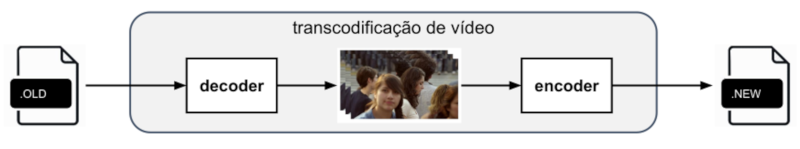
\includegraphics[width=\textwidth]{FIGURES/fig_3.png}
    \caption{Visão em alto nível de um transcodificador de vídeo original. Fonte: Elaborada pelo autor.}
    \label{fig:3}
\end{figure}

Atualmente, na era das tecnologias digitais, há dois tipos fundamentais de transcodificadores: heterogêneos e homogêneos. Eles são facilmente identificados ao se observar quais são os formatos utilizados em uma transcodificação: caso OLD e NEW sejam iguais, trata-se de uma transcodificação homogênea; caso contrário, uma transcodificação heterogênea. Apesar da transcodificação homogênea não envolver troca no formato de codificação, é muito utilizada pela indústria de vídeos, de modo a atingir algum objetivo particular, como a redução da taxa de bits por segundo, redução da resolução, adaptação do \textit{bitstream} para diferentes configurações temporais, inserção de marca d’água, etc. Em \citet{bib:modosTranscodificacao}, o autor identificou diversas utilizações de um transcodificador de vídeo, vide Figura \ref{fig:4}.

\begin{figure}
    \centering
    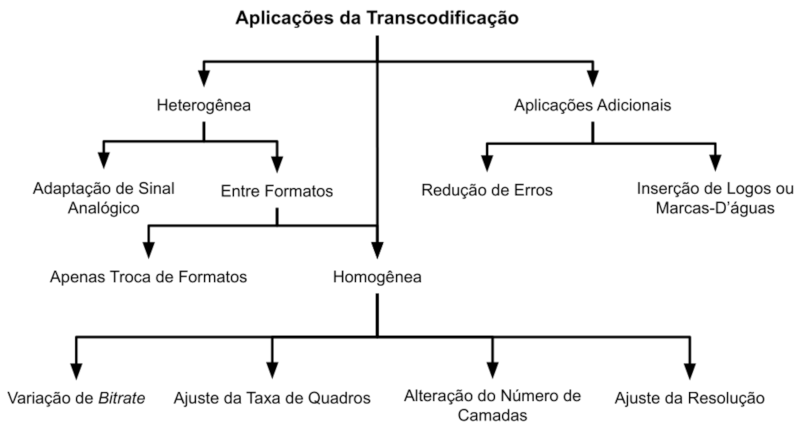
\includegraphics[width=\textwidth]{FIGURES/fig_4.png}
    \caption{Classificação de transcodificadores de vídeo. Fonte: Elaborada pelo autor com base em \citet{bib:modosTranscodificacao}.}
    \label{fig:4}
\end{figure}

Na literatura científica, a transcodificação homogênea é apresentada, principalmente, como solução para a redução da taxa de bits do vídeo (também identificado como \textit{transrating}), como no trabalho de \citet{bib:nam_2006}, mas também para a redução da resolução do vídeo, como em \citet{bib:nguyen_2015}. Esta última modalidade, que pode ser identificada como \textit{downscaling}, visa adequar a resolução original do vídeo para os mais diversos meios de reprodução que o usuário possa utilizar, já que, quando a resolução do vídeo é reduzida, a taxa de bits também o é. A preocupação com a redução do tamanho do \textit{bitstream} de forma a se adequar à largura de banda na transmissão de vídeo pode ser observada desde os princípios da internet, como pode ser visto nos trabalhos de \citet{bib:shen_1997} e \citet{bib:swann_1996}, que propuseram soluções de transcodificação para adequar o \textit{bitstream} a diferentes meios de transmissão de dados, de forma a apresentar o menor erro possível na transmissão do vídeo e manter a experiência do usuário relativamente adequada. Como na transcodificação homogênea o software codificador opera com o mesmo formato de codificação que o decodificador, a diferença entre as versões do \textit{bitstream} está em particularidades da codificação, isto é, nas configurações utilizadas.

Já a transcodificação heterogênea visa de fato a mudança no formato de codificação de vídeo usado. Uma das principais razões para se aplicar esse tipo de transcodificação é permitir a compatibilidade de um vídeo com diferentes sistemas de reprodução. Em outras palavras, um vídeo codificado com tecnologias recentes que precisa ser reproduzido em sistemas antigos (\textit{backward compatibility}) ou um vídeo codificado com tecnologias antigas que precisa ser atualizado para reprodução em sistemas mais recentes (\textit{forward compatibility}). Outros motivos, como a existência de políticas de royalties associadas à reprodução de vídeos em certos formatos, também podem motivar a conversão entre formatos. A existência de múltiplos sistemas de reprodução de vídeo no mundo real é também uma razão para que empresas necessitem manter seus vídeos em mais de um formato de codificação, como é o caso do YouTube, que oferece suporte simultaneamente aos formatos H.264, VP9 e AV1 \cite{bib:bitmovin_ott_report_2020} \cite{bib:5to9google}.

Por fim, como mostra a Figura \ref{fig:4}, também há uma categoria de transcodificação para aplicações adicionais, que não busca realizar uma modificação do \textit{bitstream} propriamente dita, mas apenas incluir nele funcionalidades novas, como inserção de marca-d'água, legendas (embutidas ou não), novas opções de idioma, etc. Normalmente esse tipo de transcodificação não é comum na literatura científica, mas pode-se citar o trabalho de \citet{bib:watermark}, que visa remover marcas-d’água existentes em vídeos.

A correta categorização da transcodificação é útil em duas situações específicas: saber quais parâmetros da codificação devem ser configurados e quais informações são particularmente importantes para serem consideradas durante uma transcodificação de vídeo acelerada. Nesta tese, destacamos principalmente os trabalhos voltados para transcodificações heterogêneas, pois os custos computacionais de execução de um codificador e um decodificador se dão em escalas diferentes. O codificador deve considerar todas as opções disponíveis no formato de codificação a fim de encontrar a melhor combinação de decisões para cada região do vídeo, gerando assim um \textit{bitstream} com a maior eficiência de codificação possível. O decodificador, por sua vez, precisa apenas reverter o \textit{bitstream} em arquivo de vídeo. Logo, havendo a possibilidade de reduzir o custo computacional ao executar o codificador, ela deve ser aproveitada.

Observa-se o emprego de quatro estratégias para realizar a transcodificação rápida:

\begin{itemize}
    \item A partir do reaproveitamento de informações provenientes exclusivamente do decodificador, com soluções baseadas em heurísticas;
    
    \item A partir do reaproveitamento de informações provenientes tanto do decodificador como do codificador, com soluções baseadas em heurísticas;

    \item A partir do reaproveitamento de informações provenientes exclusivamente do decodificador, com soluções baseadas em modelos preditivos treinados por aprendizado de máquina;

    \item A partir do reaproveitamento de informações provenientes tanto do decodificador como do codificador, com soluções baseadas em modelos preditivos treinados por aprendizado de máquina.
\end{itemize}

Apesar de todas as opções acima serem representáveis pela Figura \ref{fig:5}, a origem dos reaproveitamentos na figura leva em conta apenas informações extraídas do decodificador. Todavia, também é possível o reaproveitamento de informações provenientes do próprio codificador.

\begin{figure}
    \centering
    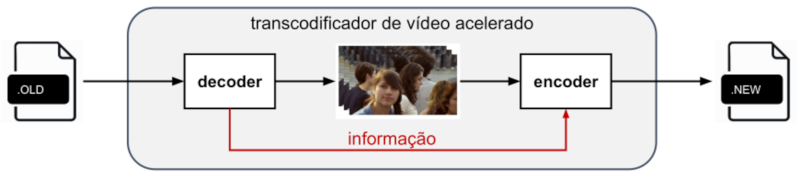
\includegraphics[width=\textwidth]{FIGURES/fig_5.png}
    \caption{Representação em alto nível de uma transcodificação rápida de vídeo. Fonte: Elaborada pelo autor.}
    \label{fig:5}
\end{figure}

Independentemente da classificação de transcodificador rápido que se faz uso, existe, em todas elas, a possibilidade de obter os dados provenientes do processo de decodificação, sendo possível transformá-los em conhecimento sobre o vídeo que será codificado. Portanto, esse conhecimento deve ser utilizado para realizar otimizações no processo decisório da codificação, com o objetivo primário de reduzir o custo computacional de executar a transcodificação e, sempre que possível, com o menor impacto na eficiência de codificação.

Assim sendo, no capítulo \ref{cap:3}, serão apresentados trabalhos publicados na literatura científica que propõem estratégias para acelerar o processo de transcodificação de vídeo. A ideia comum entre eles é o reaproveitamento de informações extraídas da decodificação (e, eventualmente, também do codificador), com ou sem uso de tratamento de dados. Dessa forma, é possível remover total ou parcialmente algumas decisões do codificador, reduzindo seu custo computacional. Para possibilitar essa aceleração, usualmente são implementadas heurísticas que relacionam os dados previamente capturados com a decisão que precisa ser realizada na codificação. Essas heurísticas podem ter, basicamente, dois tipos de embasamento: (1) através de modelos de análises estatísticas e (2) através de modelos preditivos treinados com técnicas de aprendizado de máquina. 

Diferentemente do que ocorre na transcodificação homogênea, na qual a similaridade entre dados extraídos da decodificação e decisões realizadas na recodificação são altamente correlacionados, o que possibilita o desenvolvimento de modelos heurísticos baseados em análises estatísticas de forma mais simplificada, o mesmo não ocorre na transcodificação heterogênea. Logo, um dos principais desafios na aceleração desta envolve o processo de compatibilizar as estruturas de informação e tipos de dados herdados do decodificador e os utilizados pelo codificador. Quanto maior o desafio de compatibilização, maior é a dificuldade de se acelerar um transcodificador baseado em análises estatísticas de forma eficiente. Essa é uma das razões pelas quais trabalhos com ênfase no uso de modelos de aprendizado de máquina para transcodificação de vídeo têm ganhado destaque nos últimos anos, já que esses modelos permitem a descoberta de relações entre um número maior de variáveis de forma mais eficaz que um ser humano. Portanto, na seção \ref{cap:2.2} apresentaremos uma visão geral sobre técnicas de aprendizado de máquina.

\section{Aprendizado de Máquina}
\label{cap:2.2}

É possível notar que, nos últimos anos, houve um expressivo aumento do uso de técnicas de inteligência artificial (do inglês, \textit{artificial intelligence}, AI) e de aprendizado de máquina (do inglês, \textit{machine learning}, ML) em diversas áreas da computação. Uma das grandes vantagens de utilizar técnicas de aprendizado de máquina é garantir que associações entre variáveis independentes possam ser encontradas de forma dinâmica, sem depender de instruções humanas explícitas \citet{bib:livroRaschka}. Estratégias de ML para aprender com dados disponíveis são benéficas para a solução de problemas, principalmente quando estes possuem grande volume de dados, como é o caso da codificação de vídeo. Quanto maior a quantidade e a variedade de informações disponíveis para tomada de decisão, maior é a dificuldade de encontrar relações úteis utilizando apenas a estatística e isso pode ser contornado com o uso de modelos de aprendizado de máquina.

Conforme descrito em \citet{bib:livroRaschka}, o uso de modelos de aprendizado de máquina é possível seguindo alguns passos facilmente identificáveis em quatro fases principais, como bem exemplificado na Figura \ref{fig:6}: 

\begin{figure}
    \centering
    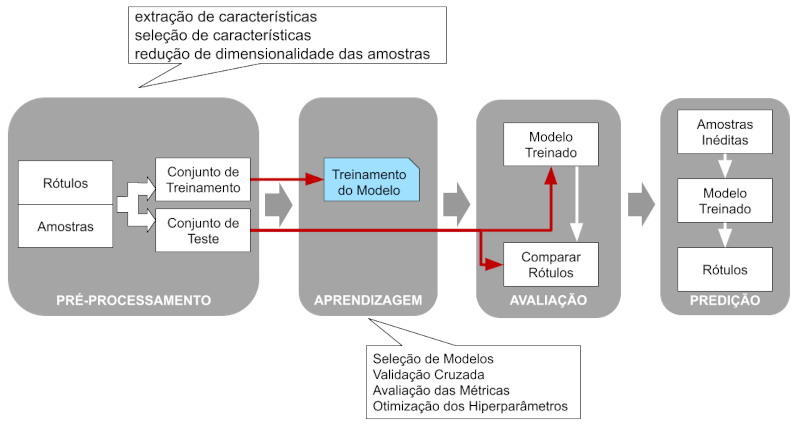
\includegraphics[width=\textwidth]{FIGURES/fig_6.png}
    \caption{Fases da vida de um modelo de aprendizado de máquina supervisionado. Fonte: Elaborada pelo autor com base em \citet{bib:livroRaschka}.}
    \label{fig:6}
\end{figure}

\begin{enumerate}[(i)]
    \item pré-processamento de dados;

    \item aprendizado;

    \item validação dos resultados;

    \item predição.
\end{enumerate}

É na primeira fase em que ocorre a extração dos dados brutos e a preparação destes para serem processados pelo algoritmo de ML. Esses dados dificilmente oferecem algum tipo de informação útil para que um modelo consiga gerar conhecimento; é necessário lapidá-los de forma a possibilitar que informações padronizadas sejam extraídas deles. Por essa razão, esta fase tende a ser uma das mais custosas de todo o ciclo de vida do uso de um modelo de aprendizado de máquina. Após a finalização da organização dos dados é que poderemos dividi-los em subconjuntos úteis para as demais fases: 

\begin{enumerate}[(a)]
    \item dados de treinamento;

    \item dados de teste;

    \item dados de validação.
\end{enumerate}

O primeiro subconjunto de dados é particularmente importante, pois é com ele que alimentamos o treinamento do modelo de aprendizado de máquina (fase (ii) do ciclo de vida). Neste conjunto, constam todos os dados válidos para treinamento (denominados atributos) e a respectiva resposta esperada para esses dados (também denominado rótulo). O segundo subconjunto é utilizado para verificar o quanto o modelo aprendeu com os dados de treinamento (fase (iii) do ciclo de vida). Basicamente, expõe-se o modelo aos dados de entrada inéditos e comparam-se os resultados de saída com os esperados para aqueles conjuntos de dados de entrada, possibilitando que se calcule a confiabilidade do modelo. É particularmente importante que os dados de treinamento e de teste sejam diferentes, afinal estamos utilizando um modelo de aprendizado de máquina para solucionar problemas desconhecidos, e não para explorar o que ele já conhece. Outro subconjunto de dados que pode ser utilizado é o de validação. Este é essencialmente similar ao subconjunto de dados de testes, só que com uma menor quantidade de dados, usados principalmente para verificar e ajustar os hiperparâmetros do modelo (explicaremos nos próximos parágrafos), quando necessário. O subconjunto de dados de validação é empregado interativamente com o conjunto de dados de treinamento, ainda na fase (ii) do ciclo de vida. Por fim, a fase (iv) do ciclo de vida é, em essência, a aplicação do modelo a situações reais, nas quais não há conhecimento prévio das saídas esperadas.

Há diversos algoritmos de aprendizado de máquina, classificados de acordo com sua forma de aprendizado \cite{bib:livroML} \cite{bib:livroKubat}. No \textbf{Aprendizado Supervisionado}, o resultado esperado (seja um dado categórico, seja um dado numérico) é conhecido e faz parte do conjunto de dados utilizados no processo de treinamento, conforme exemplos de dados apresentados anteriormente. Por outro lado, quando não há um resultado esperado ou quando este não é conhecido previamente ao processo de treinamento, empregam-se os modelos de \textbf{Aprendizado Não-Supervisionado}, cujo objetivo principal consiste justamente em encontrar as categorias ou valores que definem os dados de entrada, sendo especialmente útil para quando o objetivo do modelo é explorar os dados a fim de descobrir informações não óbvias. Por fim, há os modelos de \textbf{Aprendizado por Reforço}, em que o algoritmo aprende com os dados e se ajusta reiteradamente, utilizando mecanismos para atribuir penalidades (de modo a minimizar o erro) e recompensas (de modo a maximizar os acertos) ao longo das interações; isso possibilita que o modelo seja capaz de tomar decisões cada vez melhores, dentro de um ambiente dinâmico.

Sendo assim, quando observamos as classificações de aprendizado de máquina, conforme sua forma de aprendizado, e uma possível aplicação desses modelos em codificadores de vídeo, intuitivamente supomos que os modelos de aprendizado supervisionado sejam utilizados, uma vez que as decisões que podem ser tomadas já são conhecidas. Ou seja, apesar da elevada complexidade de um codificador de vídeo, as diversas etapas que o compõem possuem um rol limitado de opções de escolha; logo, modelos de aprendizado supervisionado são os mais adequados a esse contexto. Isso não significa que os demais algoritmos de aprendizado de máquina não possam ser aplicados a codificadores de vídeo, apenas que é menos comum.

Por fim, cabe definir o termo hiperparâmetro, que será utilizado nas próximas seções. Os hiperparâmetros são utilizados para configurar o funcionamento de algoritmos de aprendizado de máquina, tornando possível a geração de diferentes modelos preditivos com os mesmos dados de entrada. Cada algoritmo de aprendizado de máquina possui um conjunto de hiperparâmetros que podem ser configurados, como, por exemplo,a profundidade máxima das árvores treinadas em algoritmos do tipo árvore de decisão. Existe um grande número de hiperparâmetros que podem ser configurados em cada algoritmo e cada conjunto de configurações de hiperparâmetros é denominado combinação de hiperparâmetros. Alguns autores denominam essa combinação de hiperparâmetros como combinação candidata. Esta será também a nomenclatura adotada nas seções desta tese que tratam de soluções baseadas em aprendizado de máquina supervisionado.

\subsection{Aprendizado de Máquina Supervisionado}
\label{cap:2.3}

Como foi possível observar no início do capítulo \ref{cap:2}, a execução de um codificador de vídeo requer um elevado custo computacional, principalmente quando se utilizam codificadores baseados em formatos ou padrões mais atuais. Em parte, isso se relaciona com o aumento da complexidade das técnicas implementadas para realizar as predições e as compressões de dados. Uma das formas implementadas para reduzir o custo computacional é por meio do uso de algoritmos de aprendizado de máquina para acelerar tomadas de decisão do codificador. Dessa maneira, também se espera que o mesmo aconteça quando se utilizam transcodificadores de vídeo em que o conjunto de dados presentes durante o fluxo de execução do transcodificador pode ser reaproveitado pelos algoritmos de aprendizado de máquina. Como ficou mais claro na seção \ref{cap:2.2}, na área de codificação de vídeo, usam-se principalmente (mas não exclusivamente) os algoritmos de aprendizado supervisionado, já que é possível estruturar o conjunto de dados de treinamento em concordância com o rótulo de saída esperado.

Importante ressaltar que os rótulos de saída já são conhecidos, pois é possível executar o processo de codificação ou de transcodificação original de modo a se obter os valores durante e após a sua execução, o que justifica a maior presença dessa categoria de aprendizado de máquina nos trabalhos existentes na literatura científica. Como será explorado com mais detalhes no capítulo \ref{cap:3}, os algoritmos de aprendizado de máquina mais utilizados nos trabalhos de transcodificação de vídeo se baseiam em um dos três principais conceitos: árvores de decisão, classificadores lineares ou aprendizagem profunda.

O conceito de aprendizado de máquina baseado em árvore de decisão engloba algoritmos que geram uma estrutura de sequência de condicionais que parte do teste principal (com o atributo de maior relevância) até as respostas finais (folhas da árvore). Em razão disso, é facilmente implementável, tanto em software como em hardware, pois o treinamento e a execução do modelo não apresentam dificuldades. Podemos encontrar alguns algoritmos baseados em árvore de decisão, sendo que os mais comuns são o C4.5 \cite{bib:quinlan_2014}, o C5.0 \cite{bib:quinlan_2020} e o \textit{Random Forest} \cite{bib:breiman_2001}, além da versão de código aberto do C4.5, o J48.

Já os modelos baseados em classificador linear não são tão simples de ser treinados, pois se espera que os dados estejam, de alguma forma, agrupados em subconjuntos. Os algoritmos dessa classe tentam gerar uma equação algébrica capaz de separar um universo de N planos em regiões, no qual cada região corresponde a uma resposta final. Sendo assim, os modelos gerados a partir deles são mais difíceis de serem implementados. Contudo, \citet{bib:livroKubat} afirma que esse conceito de aprendizado de máquina é mais adequado para ser utilizado em conjuntos de dados com atributos mutuamente independentes. Fazem parte desse conceito os algoritmos \textit{Linear Discriminant Function} (LDF) \cite{bib:shumway_1974}, \textit{Support Vector Machine} (SVM) \cite{bib:hearst_1998} e o classificador linear \textit{Naïve-Bayes} \cite{bib:lewis_1998}.

Por fim, podemos encontrar entre os trabalhos de transcodificação de vídeo o uso de modelos de aprendizagem profunda (do inglês, \textit{Deep Learning}), cujo diferencial é a exigência de um grande número de dados para treinamento, o que eleva consideravelmente o custo computacional para utilizá-lo e exige um espaço de armazenamento alto. Apesar da probabilidade de acerto desses algoritmos serem muito interessantes, seu uso torna-se difícil em ambientes de restrição energética ou em soluções implementadas em hardware. Como veremos no capítulo \ref{cap:3}, na literatura científica em transcodificação de vídeo, poderemos encontrar soluções que empregam os algoritmos \textit{Convolutional Neural Network} (CNN) \cite{bib:koushik_2016} e \textit{Long Short-Term Memory} (LSTM) \cite{bib:graves_2012}.

Diante de tantas opções de conceitos e algoritmos de aprendizado de máquina, o número de possíveis modelos treinados para solucionar um mesmo problema é exponencial, já que cada nova possibilidade é um fator multiplicador a todas as combinações já consideradas. Por consequência, é preciso saber quais deles são mais ou menos apropriados para resolver determinados problemas. Para possibilitar a averiguação da viabilidade desses modelos, temos que mensurar a confiabilidade de cada um deles, conforme veremos na próxima seção.

\section{Confiabilidade dos Modelos de Aprendizado de Máquina}
\label{cap:2.4}

Inserir um conjunto específico de dados na entrada de um modelo de aprendizado de máquina, capturar sua resposta e compará-la com a resposta esperada é a forma mais simples de verificação da exatidão da resposta desse modelo. No entanto, um único caso de teste não é estatisticamente válido, por isso, utilizam-se diversos casos, preferencialmente diferentes dos utilizados para treinamento. A média de acertos ($\mu$), definida pela Equação \ref{eq:1}, é pouco empregada de forma isolada na literatura científica, pois não informa muito sobre que tipos de acertos e erros foram performados.

\begin{equation}
    \label{eq:1}
    \mu = \frac{acertos}{total}
\end{equation}

Aqui é importante definir que os modelos de aprendizado de máquina podem retornar respostas complexas. Contudo, para facilitar as explicações desta seção, consideramos modelos cujas respostas sejam valores binários. Inclusive, essa é a forma mais comum de respostas que se observam nos trabalhos com codificação de vídeo. Assim exposto, são esperados quatro tipos de respostas de qualquer modelo com decisões binárias: 

\begin{enumerate}[a)]
    \item \textbf{Verdadeiros Positivos} (VP), ou seja, o modelo retorna positivo quando a resposta de fato é positiva;
    
    \item \textbf{Verdadeiros Negativos} (VN), ou seja, o modelo retorna negativo quando a resposta de fato é negativa;
    
    \item \textbf{Falso Negativo} (FN), quando o modelo retorna negativo quando deveria ter retornado positivo;
    
    \item \textbf{Falso Positivo} (FP), quando o modelo retorna positivo quando deveria ter retornado negativo.
\end{enumerate}

É importante ressaltar que, em modelos cuja decisão possue um rótulo não-binário, esses quatro tipos de resposta ainda estão presentes, mas distribuídos em $2^{rotulos}$ subtipos. Nesta tese, não abordamos avaliações dessa complexidade, mas as referências para tal estão disponíveis em \citet{bib:livroKubat}, \citet{bib:livroML} e \citet{bib:livroRaschka}. Segundo essas referências, as quatro respostas de um modelo binário resultam na matriz de confusão (do inglês, \textit{confusion matrix}), representada na Tabela \ref{tab:II}, na qual, na diagonal, estão as respostas corretas e, nas demais células, estão as respostas erradas.

\begin{table}
\begin{center}
\caption{Matriz de confusão das respostas de um modelo de aprendizado de máquina.}
\label{tab:II}
\footnotesize

\begin{tblr}{
    colspec = {c|c|c|c},
    hlines,
    row{even} = {gray9}
}
\hline
\SetCell[c=2,r=2]{}&& \SetCell[c=2]{c}\textbf{Rótulos Preditos} \\
&& \textbf{Positivo} & \textbf{Negativo} \\
\SetCell[r=2]{c}\textbf{Rótulos Esperados} & \textbf{Positivo} & VP & FN \\
 & \textbf{Negativo} & FP & VN \\
\hline
\end{tblr}
\end{center}
\end{table}


Com essa matriz de confusão, é possível estabelecer o desbalanceamento da predição feita pelo modelo. É esperado que, na diagonal, os valores sejam elevados. No entanto, saber se o modelo tende a errar mais em falsos positivos ou falsos negativos pode ajudar o pesquisador a definir melhorias ou identificar relações ocultas entre as respostas preditas e esperadas. E não apenas isso: também pode ajudá-lo a identificar se o modelo treinado de fato é apto para ser utilizado em um determinado contexto. Por exemplo, no caso de um modelo em treinamento para identificar a contaminação de paciente por COVID-19, um elevado número de falsos negativos em relação a falsos positivos seria péssimo, pois pessoas infectadas poderiam ser liberadas ao convívio social, acarretando um grave problema de saúde pública. Um segundo exemplo, em que os valores de falso positivo sejam maiores que os falsos negativos, pode ser particularmente ruim caso o modelo esteja sendo utilizado para identificar a venda de ações na bolsa de valores. Nota-se que, apesar de os tipos de rótulos serem os mesmos, o contexto em que estão inseridos é de extrema importância. Demonstramos, assim, que definir e avaliar a confiabilidade do modelo não é tarefa trivial.

Por essa razão, existem diversas métricas baseadas nessa matriz de confusão, cada uma mais adequada para identificar características específicas ao contexto desejado. São elas:

\textbf{Nível de Acurácia} (do inglês, \textit{Accuracy}): Em essência, é a média apresentada na Equação \ref{eq:1}. O nível de acurácia apresenta uma relação entre as respostas corretas e todas as respostas que o modelo prediz. No contexto da matriz de confusão, a acurácia é calculada conforme a Equação \ref{eq:2}:

\begin{equation}
    \label{eq:2}
    accuracy = \frac{VN+VP}{VN+VP+FN+FP}
\end{equation}

\textbf{Nível de Precisão} (do inglês, \textit{Precision}): Informa quantas respostas corretas o modelo apresentou, considerando apenas as classificadas como verdadeiras. Essa métrica é principalmente útil quando o número de FP é mais prejudicial que o número de FN, vide exemplo da bolsa de valores mencionado anteriormente. A precisão pode ser calculada conforme a Equação \ref{eq:3}:

\begin{equation}
    \label{eq:3}
    precision = \frac{VP}{VP+FP}
\end{equation}

\textbf{Nível de Sensibilidade} (do inglês, \textit{Sensitivity}): Informa quantos rótulos existentes são verdadeiramente positivos. É uma métrica particularmente útil para identificar o quão bom um modelo treinado poderá ser em detectar respostas corretas. A sensibilidade poderá ser calculada conforme a Equação \ref{eq:4}:

\begin{equation}
    \label{eq:4}
    sensitivity = \frac{VP}{VP+FN}
\end{equation}

\textbf{Nível de Especificidade} (do inglês, \textit{Recall}): Enquanto o nível de sensibilidade informa sobre os casos positivos, o nível de especificidade informa o quão bom o modelo poderá ser em identificar os verdadeiros casos negativos. A especificidade pode ser calculada conforme a Equação \ref{eq:5}:

\begin{equation}
    \label{eq:5}
    recall = \frac{VN}{VN+FP}
\end{equation}

\textbf{Pontuação F1} (do inglês, \textit{F1-Score}): Se as métricas de precisão e sensibilidade informam, cada uma, o quão bom o modelo poderá ser em identificar casos verdadeiramente positivos e negativos, respectivamente, a métrica F1 unifica as duas métricas anteriores em um só valor. Dessa forma, facilita a relação geral do modelo em realizar boas predições binárias. O F1 poderá ser calculado por meio da média harmônica apresentada na Equação \ref{eq:6}:

\begin{equation}
    \label{eq:6}
    f1 = 2*\frac{precision*sensitivity}{precision+sensitivity}
\end{equation}

\textbf{Área sob a Curva ROC} (do inglês, \textit{Area Under the Curve}, AUC): Existe um gráfico denominado Características Operacionais do Receptor (do inglês, \textit{Receiver Operating Characteristics}, ROC), que apresenta, de forma gráfica (linha azul da Figura \ref{fig:8}), o desempenho de um modelo em classificar dados binários. Para tanto, relaciona as probabilidades da sensibilidade e o inverso da especificidade, ou seja, a relação entre os verdadeiros positivos e os falsos positivos. Assim, é possível extrair a área sob a curva ROC (área amarela da Figura \ref{fig:8}), por meio de um cálculo integral, e representar numericamente a relação apresentada no gráfico. A métrica AUC apresenta uma estimativa de desempenho de classificação do modelo ao considerar as taxas que o modelo prediz como verdadeiras e os valores reais desses rótulos. Em outras palavras, a AUC informa a probabilidade de o modelo retornar uma resposta positiva corretamente. Lembrando que ROC considera apenas valores binários, respostas aleatórias (reta laranja da Figura \ref{fig:8}) retornam 0,5 e um modelo capaz de acertar todas as respostas retorna 1,0. Portanto, a AUC informa algum valor entre esses dois limites, já que AUC inferior a 0,5 indica um péssimo modelo preditivo. A métrica AUC é especialmente útil para comparar modelos diferentes.

\begin{figure}
    \centering
    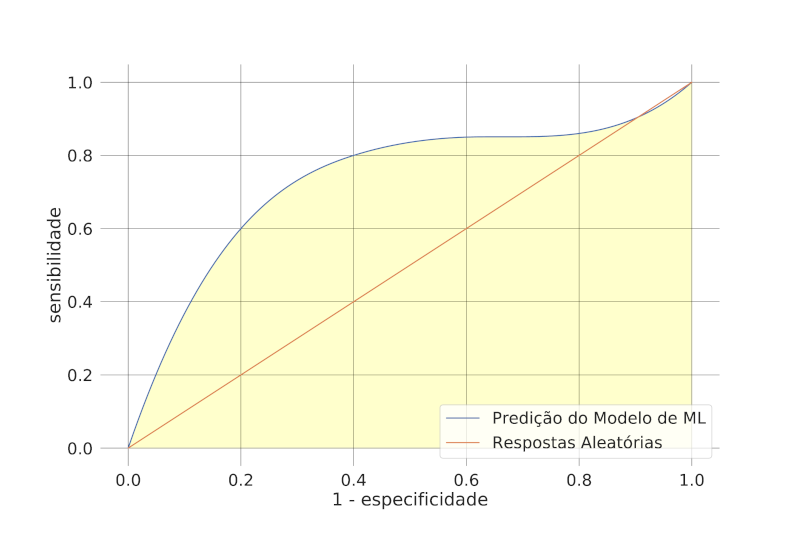
\includegraphics[width=0.85\textwidth]{FIGURES/fig_8.png}
    \caption{Exemplo da curva ROC e AUC (destacada em amarelo). Fonte: Elaborada pelo autor.}
    \label{fig:8}
\end{figure}

Outras métricas estatísticas também podem ser utilizadas, tais como t-\textit{Student} ou valor-\textit{p}, conforme \citet{bib:livroML} e \citet{bib:livroKubat}. Todavia, com menor probabilidade de uso. Dessa forma, apenas as métricas apresentadas acima são consideradas ao longo desta tese e, em particular, as métricas \textit{F1-Score} e AUC, por apresentarem maior confiabilidade nos resultados verdadeiramente válidos.

\section{Comparando Codificações}
\label{cap:2.5}

Para finalizar este capítulo, é de especial interesse abordar a forma como é feita a comparação entre duas codificações de vídeo diferentes. De forma geral, três valores são capturados durante uma codificação de vídeo: 

\textbf{Taxa de bits por segundo} (do inglês, \textit{bits per second}, bps): representa quantos bits ou kilobits (kb) o \textit{bitstream} gerado possui divididos pelo tempo em segundos do vídeo. Como esse valor é relativo à quantidade de quadros processados, a maioria dos codificadores já fornece esse valor médio.

\textbf{Nível da qualidade da imagem}: indica a diferença objetiva entre a imagem original (pré-codificada) e a imagem decodificada (pós-codificada). Existe, na literatura, uma série de métricas objetivas que capturam a diferença entre as duas imagens, sendo as mais comuns a Relação Sinal-Ruído de Pico (do inglês, \textit{Peak Signal-to-Noise Ratio}, PSNR) \cite{bib:psnr} e a Fusão de Vários Métodos de Avaliação de Vídeo (do inglês, \textit{Video Multi-Method Assessment Fusion}, VMAF) \cite{bib:vmaf}. O valor da métrica PSNR, assim como a taxa de bits, já é fornecido pela maioria dos codificadores após a codificação. Portanto, é a mais usual de ser encontrada na literatura científica, apesar das diversas inconsistências que essa métrica oferece quando comparada com métricas subjetivas ou empregada em vídeos mais complexos, como HDR ou \textit{Screen Content} \cite{bib:mse_wrong}. Note que o cálculo do PSNR é sempre resultante da diferença entre a sequência de vídeo original (âncora) com a versão dessa sequência após a codificação (comparada). Além disso, na transcodificação de vídeos, o PSNR é calculado tendo-se a sequência decodificada como âncora e a sequência re-codificada como comparada.

\textbf{Variação do Tempo de Codificação}: informa a diferença percentual entre o tempo exigido para executar a codificação em observação e o tempo de codificação de referência. Os trabalhos de transcodificação de vídeo apresentados nesta tese visam sempre apresentar um tempo de codificação inferior ao de referência. Portanto, normalmente se apresentam valores de Redução de Tempo (do inglês, \textit{Time Saving}, TS). Para o cálculo da redução do tempo de codificação ou de transcodificação, utilizamos a Equação \ref{eq:7}, onde $Ta$ e $Tb$ são os tempos de codificação original e modificada, respectivamente, e $q$ representa o conjunto de níveis de quantização utilizados.

\begin{equation}
    \label{eq:7}
    TS = 100 * \left ( \frac{1}{n} \sum_{q_0}^{q_n} \frac{Ta_q - Tb_q}{Ta_q} \right )
\end{equation}

É importante destacar que existe uma relação entre a taxa de bits por segundo e o nível da qualidade da imagem, isto é, uma maior quantidade de dados permite armazenar vídeos com maior qualidade de imagem. Ao mesmo tempo, codificadores de vídeo mais modernos são capazes de comprimir vídeos com idêntico nível de qualidade de imagem que outro codificador mais antigo, mas com uma quantidade inferior de dados. Portanto, essa relação entre taxa de bits e qualidade de imagem precisa ser considerada ao se realizar comparações entre diferentes codificadores ou variações de um mesmo codificador. O principal destaque a ser feito é que os níveis de qualidade da imagem também são alterados, o que dificulta a correlação direta nessas comparações.

Dessa forma, \citet{bib:bdrate} desenvolveu uma métrica, denominada Bj{\o}ntegaard Delta(BD)-rate, que relaciona duas codificações diferentes sob a ótica dessas duas variáveis alvo. Para tanto, faz uso do cálculo de uma integral que representa a área entre duas curvas de taxa de bits e nível de qualidade, como apresentado na Figura \ref{fig:9}. Basicamente, o BD-rate equipara os níveis de qualidade e informa a diferença percentual da taxa de bits de uma codificação em relação à codificação de referência. Sendo assim, valores negativos indicam uma redução na taxa de bits, o que é normalmente esperado quando se comparam formatos de codificação de vídeo recentes frente aos mais antigos. Por outro lado, valores positivos de BD-rate indicam um aumento na taxa de bits, o que é mais comum ocorrer nos trabalhos de transcodificação de vídeo acelerado frente aos transcodificadores originais.

\begin{figure}
    \centering
    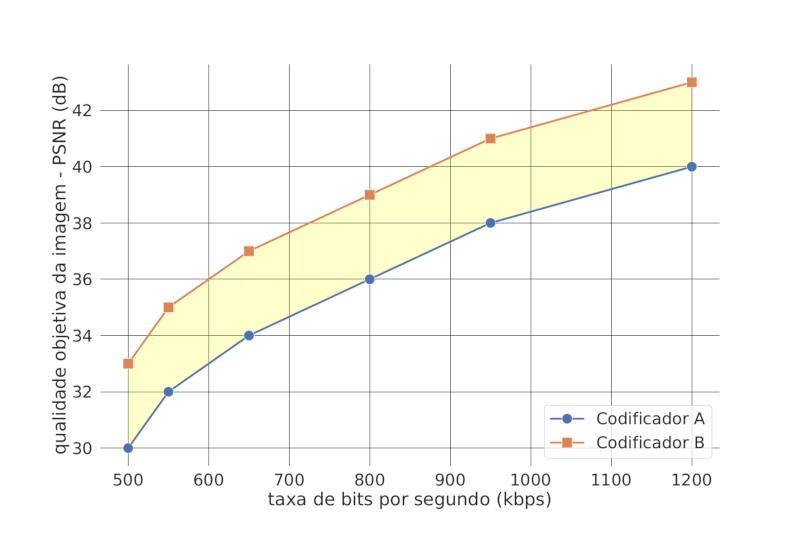
\includegraphics[width=0.85\textwidth]{FIGURES/fig_9.png}
    \caption{Exemplificando duas curvas de BD-rate. Fonte: Elaborada pelo autor.}
    \label{fig:9}
\end{figure}

Finalizamos, então, todos os conceitos básicos necessários para a compreensão do restante desta tese. Para conhecimentos mais aprofundados, recomendamos a leitura das referências bibliográficas apontadas ao longo deste capítulo. No capítulo \ref{cap:3}, apresentamos o estado da arte em transcodificação de vídeo.


\chapter{Revisão Sistemática da Literatura em Transcodificação de Vídeo}
\label{cap:3}

O objetivo principal deste capítulo é apresentar ao leitor o estado da arte da literatura científica acerca de transcodificadores rápidos de vídeo. De forma a garantir uma maior acurácia da metodologia de pesquisa da literatura científica, utilizamos o processo de Metodologia Sistemática da Literatura (MSL) \cite{bib:msl}. Segundo essa metodologia, deve-se definir bem o escopo da busca pela literatura, a fim de possibilitar a replicação desse processo o mais fielmente possível, haja vista que é esperado que ocorra alguma mudança, pois a literatura é constantemente atualizada.

Assim sendo, nesta tese, utilizamos três ferramentas de busca como fonte dos artigos acadêmicos: a IEEE Xplore, a \textit{Association for Computing Machinery} (ACM) \textit{Library} e o \textit{Google Scholar}. Em cada uma delas, realizamos as mesmas buscas, procurando a presença das palavras ``\textit{transcoding}'' e ``\textit{transcoder}'', seja no título ou no \textit{abstract}. Selecionamos para estudo os primeiros 500 artigos que cada uma das ferramentas de busca considerou mais relevantes, totalizando 1500 artigos a serem revisados.

Após a obtenção dos artigos, aplicamos filtros para remover trabalhos com as características descritas abaixo: 

\begin{enumerate}[i.]
    \item Artigos duplicados;

    \item Artigos que focam na transcodificação de dados que não vídeo – por exemplo, transcodificação de áudio;

    \item Artigos que empregam o termo ``transcodificação'' como sinônimo para outra palavra, como ``codificação'';

    \item Artigos que apresentam a transcodificação sem foco em acelerar o processo, ou seja, não possuem redução do tempo (TS) ou qualquer forma de mensurar esse valor;

    \item Artigos que não apresentam a métrica BD-rate.
\end{enumerate}

Após os quatro primeiros filtros, dos 1500 artigos capturados sobraram 140; no entanto, somente 34 deles é que passaram pelo quinto filtro. Observe que o BD-rate começou a ser utilizado na literatura científica após o ano de 2010. Portanto, existe esse recorte dos trabalhos: consideramos apenas a última década (2011-2022) de artigos publicados com foco em acelerar a transcodificação de vídeo. Isso porque a ausência do BD-rate inviabiliza qualquer discussão comparativa entre os trabalhos. De cada um dos artigos selecionados, os seguintes dados foram capturados e armazenados em uma tabela:

\begin{enumerate}[1.]
    \item Título do artigo;
    
    \item Nome dos autores;
    
    \item Código do \textit{Digital Object Identifier} (DOI);
    
    \item Nome do formato utilizado na decodificação;
    
    \item Nome do formato utilizado na recodificação;
    
    \item Estágios envolvidos na transcodificação. Os possíveis estágios a serem selecionados neste campo são: ``predição intraquadro'', ``predição interquadros'', ``transformada'', ``quantização'', ``codificação de entropia'', ``filtros'', ``particionamento de blocos'' e ``outros'';
    
    \item Nome do algoritmo de aprendizado de máquina utilizado, quando existente;
    
    \item Breve descrição da proposta apresentada no trabalho.
\end{enumerate}

Com os artigos devidamente catalogados, torna-se possível apresentar o estado da arte da transcodificação de vídeo com foco na redução do custo computacional. Para facilitar essa apresentação, categorizamos os trabalhos em três tópicos: visão geral da transcodificação de vídeo (seção \ref{cap:3.1}); transcodificação assistida por aprendizado de máquina (seção \ref{cap:3.2}) e transcodificação acelerada por herança de particionamento de blocos (seção \ref{cap:3.3}).

Entre os trabalhos selecionados, é possível observar uma prevalência de soluções para transcodificação de ``origem'' ou para ``destino'' o formato H.265/HEVC. Aproximadamente 85\% de todos os trabalhos selecionados incluem soluções que visam adaptar vídeos codificados no padrão H.265/HEVC para tecnologias mais antigas (como H.264/AVC) ou para tecnologias mais recentes (como H.266/VVC). Tendo em vista que o escopo do estudo do estado da arte apresentado está entre os anos de 2011 e 2022, torna-se compreensível que o H.265/HEVC tenha sido o formato de vídeo mais estudado na literatura, pois o H.265/HEVC foi o padrão de codificação de vídeo estado-da-arte desde seu lançamento em 2013 até 2020, quando o H.266/VVC foi lançado. O segundo formato de vídeo que mais aparece na literatura selecionada é o H.264/AVC, com presença de 63\% entre todos os artigos, seguido pelo AV1 (15\%). Esses dois codificadores de vídeo são amplamente utilizados para fins comerciais hoje em dia, principalmente para transmissões de vídeos pela internet. Portanto, já esperávamos que tivessem destaque especial na literatura.

Considerando os tipos de transcodificações apresentados em \cite{bib:modosTranscodificacao} (vide Figura \ref{fig:4}), podemos encontrar, na literatura selecionada, dois tipos principais de trabalhos: transcodificações heterogêneas (78\%) e transcodificações homogêneas (22\%), sendo que esta última está subdividida em redução da taxa de bits (\textit{transrating}) e redução da resolução espacial (\textit{downscaling}). Dessa forma, essa diferença dos tipos de trabalho evidencia que a conversão entre formatos de vídeo é particularmente importante na literatura científica, assim como a adaptação da taxa de bits e o controle da resolução do vídeo, principalmente ao se considerar a relevância dos serviços de \textit{streaming} nos dias de hoje.

Dentre todos os formatos e padrões de codificação de vídeos apresentados na Figura \ref{fig:1}, encontram-se presentes na revisão sistemática da literatura apenas os formatos H.264/AVC, H.265/HEVC, H.266/VVC, VP9, AV1 e AVS, distribuídos conforme a Figura \ref{fig:10}. Em relação à transcodificação homogênea (Figura \ref{fig:10}(a)), encontramos apenas trabalhos que propõem soluções para os formatos H.264/AVC ou H.265/HEVC, sendo que este último representa 57,14\% dos casos. Para trabalhos de transcodificação de vídeos heterogêneos, H.264/AVC também é o principal formato de origem, com presença de 61,54\% (Figura \ref{fig:10}(b)), enquanto o formato H.265/HEVC é o principal formato de destino, com 65,38\% (Figura \ref{fig:10}(c)). Portanto, é possível notar que os formatos de codificação de vídeo desenvolvidos pelo ITU-VCEG têm sido o foco principal dos pesquisadores que trabalham com transcodificação de vídeo.

\begin{figure}
    \centering
    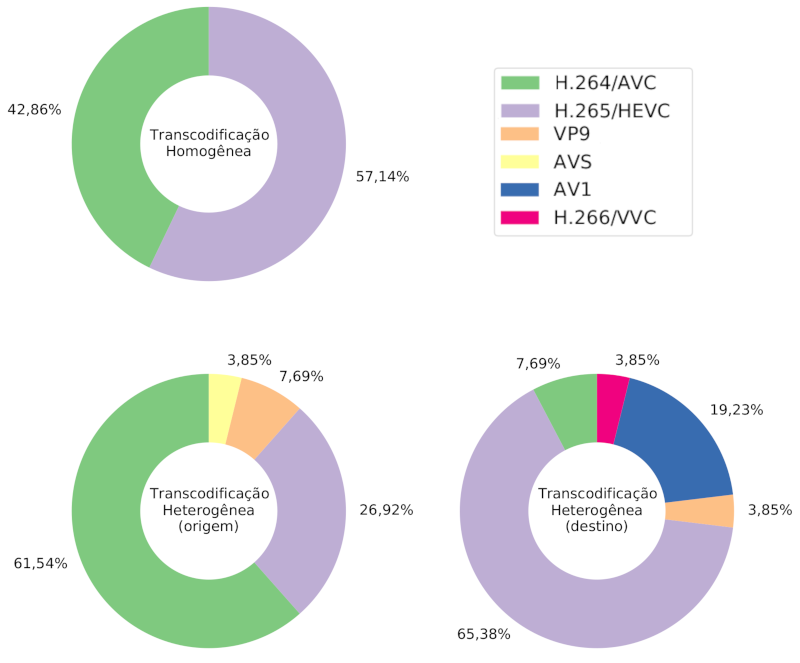
\includegraphics[width=\textwidth]{FIGURES/fig_10.png}
    \caption{Distribuição da presença dos formatos de codificação de vídeo observados na revisão sistemática da literatura, conforme o tipo de transcodificação. Fonte: Elaborada pelo autor.}
    \label{fig:10}
\end{figure}

Descrevemos os seis principais estágios de um codificador de vídeo híbrido no capítulo \ref{cap:2}, mas o particionamento de blocos também é um processo decisório importante durante a execução de um codificador. Portanto, precisa ser considerado quando se trata do estudo de complexidade daquele formato de codificação de vídeo. Ao observar a literatura selecionada, percebemos que a maioria das soluções concentram seus esforços em acelerar um transcodificador de vídeo através do processo de particionamento de blocos, como pode ser visto na Figura \ref{fig:11}. Nela, mostramos a distribuição do campo ``estágios envolvidos na transcodificação'', de acordo com os dados capturados durante a revisão da literatura. O círculo externo dessa figura representa todo o conjunto de 140 artigos revisados após os quatro primeiros processos de filtragem, ou seja, removidos os trabalhos duplicados e que não estão relacionados à transcodificação rápida de vídeo, enquanto o círculo interno representa o conjunto dos 34 artigos que, de fato, foram selecionados após o quinto processo de filtragem. Conforme mostrado no círculo interno, os estágios abordados no reaproveitamento de informações em soluções para transcodificação acelerada são: o particionamento de bloco (70,59\%), a predição interquadros (41,18\%) e a predição intraquadro (8,89\%). É notório nessa figura que os três principais tópicos de estudo são os mesmos nos dois círculos, mas com distribuições diferentes. Antes da aplicação dos dois últimos filtros, observamos outra ordem: predição interquadros (42,62\%), particionamento de blocos (18,58\%) e predição intraquadro (17,49\%).

\begin{figure}
    \centering
    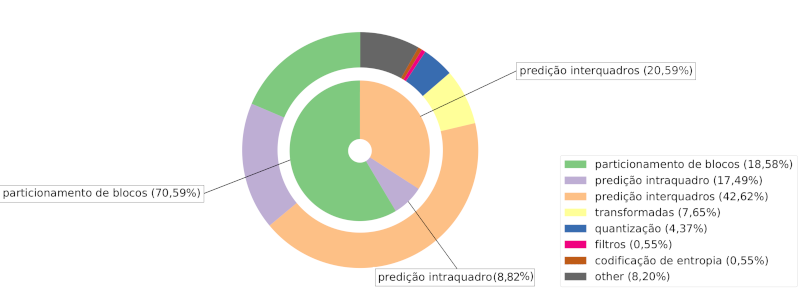
\includegraphics[width=\textwidth]{FIGURES/fig_11.png}
    \caption{Distribuição do campo ``estágios envolvidos na transcodificação'', observados durante a revisão sistemática da literatura. Fonte: Elaborada pelo autor.}
    \label{fig:11}
\end{figure}

Após essa visão geral dos trabalhos revisados, podemos apresentar, de forma mais especializada, cada um dos tópicos de interesse acerca do estado da arte em transcodificação rápida de vídeo.

\section{Visão Geral da Transcodificação Rápida de Vídeo}
\label{cap:3.1}

Os 34 artigos selecionados após as etapas de filtragem estão resumidos na Tabela \ref{tab:III}, apresentando os formatos de decodificação e de codificação utilizados, assim como as métricas BD-rate e TS para cada solução proposta. Todos eles fazem uso de heurísticas para acelerar o transcodificador, com base em análises estatísticas ou em aprendizado de máquina. Em média, os trabalhos de aceleração da transcodificação de vídeo publicados na última década são capazes de reduzir o tempo do processo de transcodificação à metade (TS médio igual à 50,74\%) em comparação com o transcodificador original correspondente. Observando o desvio padrão da redução do tempo, é seguro afirmar que existe uma grande probabilidade de que soluções de transcodificação rápida ofereçam uma redução de tempo entre 31,51\% e 69,97\%. Já o impacto médio na eficiência de codificação (em termos de BD-rate) é de 4,11\%, e não superior a 6,57\% em média (considerando desvio padrão mais a média), indicando que é esperada alguma perda na eficiência de codificação, desde pequenos a médios valores de BD-rate, ao se executar a transcodificação na metade do tempo de um transcodificador original.

\afterpage{
\clearpage

\begin{landscape}
{\footnotesize
\begin{longtblr}[
    caption = {Resumo dos artigos presentes na revisão sistemática da literatura sobre transcodificação rápida de vídeo, publicados entre os anos de 2011 e 2022.},
    label = {tab:III},
    note{1} = {Valor adaptado da métrica ``número de vezes mais rápido que'' (do inglês, \textit{speed-up}) para percentual TS.}
]{
    colspec = {p{5cm}|p{2.2cm}|p{2.2cm}|p{4cm}|c|c|c},
    rowhead = 1,
    hlines,
    row{even} = {gray9}
}
\hline
\textbf{Autor} & \textbf{Formato de Origem} & \textbf{Formato de Destino} & \textbf{Estágios Envolvidos} & \textbf{BD-rate (\%)} & \textbf{TS (\%)} & \textbf{Razão ($\frac{BD-rate}{TS}$)} \\
\citet{bib:leuven_2011} & H.264/AVC & H.264/AVC & particionamento de blocos, predição intraquadro & 7,33 & 95,73 & 0,077 \\
\citet{bib:wang_2012} & H.264/AVC & H.264/AVC & predição interquadros & 3,53 & 90,62 & 0,039 \\
\citet{bib:aminlou_2016} & H.264/AVC & H.264/AVC & predição interquadros & 6,60 & 6,80 & 0,971 \\
\SetCell[c=4]{r}\textit{Média de H.264/AVC-to-H.264/AVC} &&&& \textit{5.82} & \textit{64.38} & \\
\SetCell[c=4]{r}\textit{Desvio Padrão de H.264/AVC-to-H.264/AVC} &&&& \textit{2,02} & \textit{49,93} & \\

\citet{bib:zhang_2012} & H.264/AVC & H.265/HEVC & particionamento de blocos, predição intraquadro e predição interquadros & 30,00 & 80,00 & 0,375 \\
\citet{bib:peixoto_2012} & H.264/AVC & H.265/HEVC & predição interquadros & 5,49 & 52,74 & 0,104 \\
\citet{bib:jiang_2013} & H.264/AVC & H.265/HEVC & predição interquadros & 1,45 & 30,50 & 0,048 \\
\citet{bib:peixoto_2014} & H.264/AVC & H.265/HEVC & predição interquadros & 3,87 & 63,06 & 0,061 \\
\citet{bib:peixoto2_2014} & H.264/AVC & H.265/HEVC & particionamento de blocos & 8,41 & 70,54 & 0,119 \\
\citet{bib:honrubia_2014} & H.264/AVC & H.265/HEVC & particionamento de blocos & 4,80 & 64,29 & 0,075 \\
\citet{bib:peixoto3_2014} & H.264/AVC & H.265/HEVC & particionamento de blocos, predição intraquadro e predição interquadros & 3,32 & 49,75\TblrNote{1} & 0,067 \\
\citet{bib:nagaraghatta_2015} & H.264/AVC & H.265/HEVC & predição interquadros & 4,20 & 50,33 & 0,083 \\
\citet{bib:franche_2015} & H.264/AVC & H.265/HEVC & BP. predição interquadros & 3,28 & 87,32 & 0,038 \\
\citet{bib:honrubia_2015} & H.264/AVC & H.265/HEVC & particionamento de blocos & 5,20 & 60,00\TblrNote{1} & 0,087 \\
\citet{bib:honrubia_2016} & H.264/AVC & H.265/HEVC & particionamento de blocos & 2,20 & 57,37 & 0,038 \\
\citet{bib:correa_2016} & H.264/AVC & H.265/HEVC & particionamento de blocos & 1,67 & 44,10 & 0,038 \\
\citet{bib:franche_2017} & H.264/AVC & H.265/HEVC & predição interquadros & 10,13 & 67,90 & 0,149 \\
\citet{bib:liu_2018} & H.264/AVC & H.265/HEVC & particionamento de blocos & 1,83 & 53,71 & 0,034 \\
\citet{bib:xu_2019} & H.264/AVC & H.265/HEVC & particionamento de blocos & 1,16 & 59,60 & 0,019 \\
\citet{bib:soares_2019} & H.264/AVC & H.265/HEVC & particionamento de blocos & 0,75 & 24,28 & 0,031 \\
\citet{bib:xin_2022} & H.264/AVC & H.265/HEVC & particionamento de blocos & 0,60 & 38,40 & 0,015 \\
\SetCell[c=4]{r}\textit{Média de H.264/AVC-to-H.265/HEVC} &&&& \textit{5,20} & \textit{56,11} \\
\SetCell[c=4]{r}\textit{Desvio Padrão de H.264/AVC-to-H.265/HEVC} &&&& \textit{2,71} & \textit{15,59} \\

\citet{bib:sung_2014} & H.265/HEVC & H.265/HEVC & particionamento de blocos & 1,46 & 51,02 & 0,029 \\
\citet{bib:nguyen_2015} & H.265/HEVC & H.265/HEVC & particionamento de blocos & 0,88 & 40,50 & 0,022 \\
\citet{bib:grellert_2018} & H.265/HEVC & H.265/HEVC & particionamento de blocos & 0,29 & 41,81 & 0,007 \\
\citet{bib:lindino_2021} & H.265/HEVC & H.265/HEVC & particionamento de blocos & 0,54 & 42,00 & 0,013 \\
\citet{bib:xin_2022} & H.265/HEVC & H.265/HEVC & particionamento de blocos & 0,60 & 38,40 & 0,015 \\
\SetCell[c=4]{r}\textit{Média de H.265/HEVC-to-H.265/HEVC} &&&& \textit{5.20} & \textit{56,11} \\
\SetCell[c=4]{r}\textit{Desvio Padrão de H.265/HEVC-to-H.265/HEVC} &&&& \textit{2,71} & \textit{15,59} \\

\citet{bib:borges_2019} & H.265/HEVC & AV1 & particionamento de blocos & 4,55 & 35,41 & 0,128 \\
\citet{bib:borges2_2019} & H.265/HEVC & AV1 & particionamento de blocos & 4,94 & 35,43 & 0,139 \\
\citet{bib:chen_2019} & H.265/HEVC & AV1 & particionamento de blocos & 0,79 & 37,80 & 0,021 \\
\citet{bib:borges2_2021} & H.265/HEVC & AV1 & particionamento de blocos & 5,38 & 34,06 & 0,158 \\
\SetCell[c=4]{r}\textit{Média de H.265/HEVC-to-AV1} &&&& \textit{3,91} & \textit{35,68} \\
\SetCell[c=4]{r}\textit{Desvio Padrão de H.265/HEVC-to-AV1} &&&& \textit{2,11} & \textit{1,56} \\

\citet{bib:jin_2011} & AVS & H.264/AVC & predição intraquadro e predição interquadros & 0,58 & 78,15 & 0,007 \\
\citet{bib:tang_2015} & H.265/HEVC & H.264/AVC & particionamento de blocos, predição intraquadro e predição interquadros & 2,68 & 60,62 & 0,044 \\
\citet{bib:torre_2015} & H.265/HEVC & VP9 & predição interquadros & 3,51 & 36,24 & 0,097 \\
\citet{bib:li_2017} & VP9 & H.265/HEVC & particionamento de blocos & 3,70 & 43,50 & 0,085 \\
\citet{bib:lucas_2020} & H.265/HEVC & H.266/VVC & particionamento de blocos & 0,32 & 13,38 & 0,024 \\
\citet{bib:borges_2021} & VP9 & AV1 & particionamento de blocos & 4,34 & 28,16 & 0,154 \\
\SetCell[c=4]{r}\textbf{Média Geral} &&&& \textbf{4,11} & \textbf{50,74} \\
\SetCell[c=4]{r}\textbf{Desvio Padrão Geral} &&&& \textbf{2,46} & \textbf{19,23} \\
\hline
\end{longtblr}
}
\end{landscape}
}


Há propostas de transcodificação rápida que não estão dentro da faixa média $\pm$ desvio padrão, podendo apresentar resultados tanto positivos como negativos em relação à média. Todavia, sem haver uma análise crítica em relação aos parâmetros de configurações utilizadas por essas propostas, assim como os contextos de aplicação de cada uma das técnicas utilizadas nestas propostas, qualquer valor observado de BD-rate e TS não pode ser comparado com essa média da literatura sem ocasionar em injustiças. Dessa forma, a média observada na literatura serve apenas como uma referência probabilistica. Por exemplo, \citet{bib:jin_2011} apresenta um valor significativamente positivo ao transcodificar de AVS-para-H.264/AVC, pois sua proposta atinge uma redução de tempo de 78,15\% com uma mínima perda de eficiência de compressão (0,58\% de BD-rate). Em \citet{bib:jin_2011}, os autores propõem um \textit{downscaling} de resolução de vídeo codificado originalmente em AVS para o padrão H.264/AVC ao mapear a predição intraquadro, ou seja, propõem aplicar uma transcodificação homogênea e heterogênea ao mesmo tempo. Por outro lado, um resultado considerado negativo pode ser observado em \citet{bib:leuven_2011}, que limita a predição intraquadro e o particionamento de blocos sob certas condições. Nesse trabalho, há uma equivalência percentual entre os valores de redução de tempo e de impacto na eficiência de codificação (TS=6,8\% e BD-rate=6,6\%), o que indica uma baixa relação entre eficiência de codificação e aceleração. Isso pode ser observado na coluna Razão, na qual valores próximos de zero são ideais, pois indicam um leve aumento na taxa de BD-rate para cada ponto percentual de aceleração obtido. Além disso, essa coluna permite equacionar diferentes soluções de forma mais direta, tornando possível compará-las. Por exemplo, as soluções propostas por \citet{bib:franche_2015}, \citet{bib:honrubia_2016} e \citet{bib:correa_2016}, todas com foco na transcodificação de H.264/AVC para H.265/HEVC, apresentam resultados diferentes de BD-rate (3,28\%, 2,20\% e 1,70\%, respectivamente) e de TS (87,32\%, 57,37\% e 44,10\%, respectivamente), no entanto, são similares, já que possuem a mesma razão de 0,038.

A Figura \ref{fig:12} apresenta os trabalhos da Tabela \ref{tab:III} espalhados visualmente, onde cada ponto indica um trabalho indicado pela primeira letra do sobrenome do autor seguido do ano de publicação do trabalho; nela, o eixo horizontal representa a perda de eficiência de codificação (BD-rate) e o eixo vertical, a aceleração de transcodificação (TS). O gráfico permite visualizar os dados da Tabela \ref{tab:III}. No entanto, é de suma importância enfatizar que qualquer comparação direta entre os trabalhos não é possível, ou mesmo justa, apenas avaliando os seus resultados de BD-rate e TS, sem que se faça uma distinção entre contextos e aplicabilidades. Avaliando-se a Figura \ref{fig:12}, poderia-se supor que os pontos mais próximos da região superior esquerda forneçam as melhores relações entre redução de complexidade e eficiência de codificação, ou seja, são propostas que apresentam baixa Razão, que vai aumentando conforme os resultados se afastam dessa região. Nesta visão mais ampla, os resultados que apresentam as melhores relações de Razão foram obtidos por \citet{bib:jin_2011} e \citet{bib:grellert_2018}, todos eles com uma Razão de 0,007. Por outro lado, as duas propostas com maior Razão são \citet{bib:aminlou_2016} (Razão de 0,971) e \citet{bib:zhang_2012} (Razão de 0,375). Para melhor visualização, o trabalho de \citet{bib:zhang_2012} não foi incluído na Figura \ref{fig:12} devido ao alto valor de BD-rate (30\%).

\afterpage{
\clearpage
\begin{landscape}
\begin{figure}
    \centering
    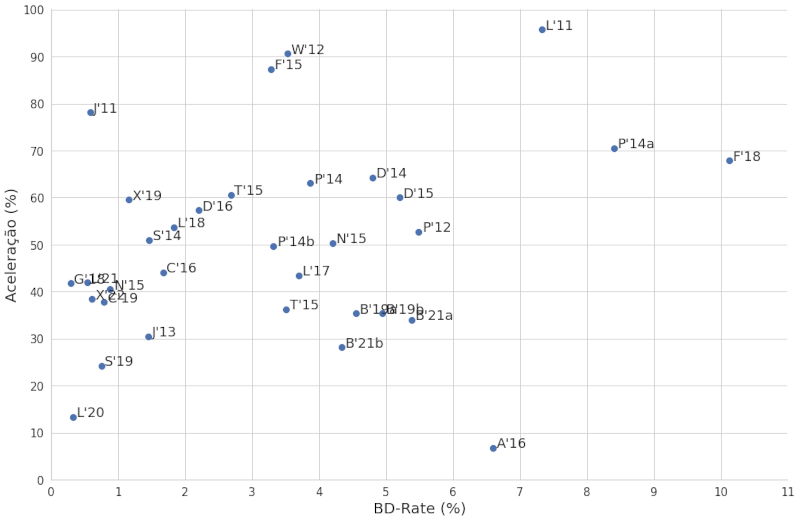
\includegraphics[width=0.8\linewidth]{FIGURES/fig_12.png}
    \caption{Valores de redução do tempo e do impacto na eficiência de codificação dos trabalhos selecionados pela revisão sistemática da literatura. Fonte: Elaborada pelo autor.}
    \label{fig:12}
\end{figure}
\end{landscape}
}


Uma análise mais aprofundada dos artigos apresentados na Tabela \ref{tab:III} permite observar que a reutilização do particionamento de blocos é a estratégia preferida para acelerar o processo de transcodificação, principalmente após o ano de 2015. Isso pode ser explicado porque o particionamento de blocos é uma tarefa essencial na codificação de vídeo, representando o principal laço de repetição do complexo processo de Otimização Taxa-Distorção (do inglês, \textit{Rate-Distortion Optimization}, RDO) \cite{bib:rdo_sullivan}, com decisões que afetam todos os estágios de codificação, direta ou indiretamente. A seção \ref{cap:3.3} cobre com mais detalhes essa categoria de soluções.

Por fim, é perceptível que a perda de eficiência de compressão diminuiu significativamente nos trabalhos publicados nos últimos anos. De fato, 70\% dos artigos da Tabela \ref{tab:III} que atingem um BD-rate inferior a 3\% empregam soluções baseadas em aprendizado de máquina para acelerar as decisões de transcodificação. Por essa razão, discutimos essa categoria de forma mais minuciosa na seção \ref{cap:3.2}.

\section{Transcodificação Assistida por Aprendizado de Máquina}
\label{cap:3.2}

O aprendizado de máquina (do inglês, \textit{Machine Learning}, ML) é um campo de pesquisa que cresceu significativamente nos últimos anos e hoje é aplicado em diversas áreas para resolver diferentes tipos de problema. Na área de codificação de vídeo, isso não é diferente, com contribuições que vão desde o desenvolvimento de novas ferramentas baseadas em aprendizado para codecs híbridos até autoencoders \cite{bib:autoencoder}, codificadores de vídeo totalmente baseados em redes neurais profundas. Quanto às soluções de transcodificação rápida, as propostas são tipicamente focadas em auxiliar as tomadas de decisão, baseando-se em dados extraídos do \textit{bitstream} decodificado e evitando, assim, o teste exaustivo do RDO para várias possibilidades de codificação. Nessas propostas, incluem-se decisões sobre: os modos de predição, a geração de vetores de movimento e a pré-definição de particionamento de blocos. Essa simplificação do processo RDO pode ser tratada como um problema de classificação, pois o modelo treinado poderá detectar: 

\begin{enumerate}[i.]
    \item um modo único a ser testado, descartando todos os restantes;
    
    \item um modo único a ser descartado, testando os demais;
    
    \item um subconjunto de modos a serem testados, descartando os demais.
\end{enumerate}

Algumas soluções de transcodificação assistida por aprendizado de máquina também são baseadas em acelerações locais no lado do codificador, usando modelos treinados com informações obtidas tanto do decodificador (formato de origem) quanto do codificador (formato de destino). Por exemplo, além dos atributos reunidos durante a decodificação, \citet{bib:lucas_2020} também usa a média e a variância dos blocos residuais obtidos durante o processo de codificação do H.266/VVC para prever o particionamento do bloco a ser utilizado. O uso de reaproveitamento de dados de origem tanto do decodificador como do codificador também pode ser observado nos trabalhos de \citet{bib:nguyen_2015}, \citet{bib:franche_2015} e \citet{bib:franche_2017}, apesar de eles não utilizarem soluções baseadas em aprendizado de máquina. Em relação ao conjunto de atributos para serem processados pelo modelo de ML, podem ser diferentes ou idênticos, mesmo para prever decisões distintas. Por exemplo, \citet{bib:peixoto_2014} e \citet{bib:li_2017} usam o mesmo conjunto de recursos em seus trabalhos. Todavia, \citeauthor{bib:peixoto_2014} os usa para prever vetores de movimento a serem utilizados no H.264/AVC, enquanto \citeauthor{bib:li_2017} utiliza esses atributos para prever o particionamento de blocos na codificação H.265/HEVC.

As soluções apresentadas nesses artigos são baseadas em diversos métodos e algoritmos de aprendizado de máquina atualmente disponíveis. As contribuições desses trabalhos na transcodificação de vídeo estão resumidas na Figura \ref{fig:13}, categorizadas de acordo com o algoritmo empregado. No círculo externo da Figura \ref{fig:13}, está a distribuição das categorias de aprendizado de máquina, enquanto, no círculo interno, está a distribuição dos algoritmos utilizados. As soluções observadas na revisão sistemática da literatura se enquadram em três categorias principais de aprendizado de máquina supervisionado \cite{bib:livroKubat}: classificação linear, árvores de decisão e aprendizado profundo, como já foi apresentado na subseção \ref{cap:2.3}.

\begin{figure}
    \centering
    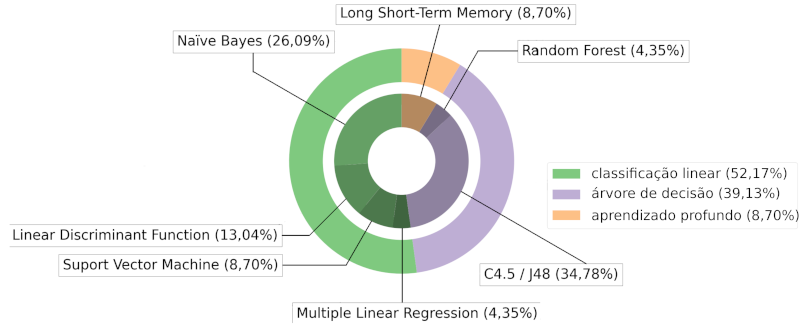
\includegraphics[width=\textwidth]{FIGURES/fig_13.png}
    \caption{Distribuição de algoritmos de aprendizado de máquina nos artigos revisados sobre aceleração de transcodificação de vídeo. Fonte: Elaborada pelo autor.}
    \label{fig:13}
\end{figure}

É possível observar, na Figura \ref{fig:13}, que o algoritmo C4.5/J48, dentro da categoria de árvores de decisão, é o mais empregado nas soluções encontradas na literatura. Por exemplo, \citet{bib:correa_2016} propõe o uso de árvores de decisão treinadas em C4.5 para prever o melhor particionamento de blocos para \textit{Coding Units} (CUs) do H.265/HEVC com base em dados coletados da decodificação do H.264/AVC. Da mesma forma, \citet{bib:escribano3_2008} emprega o mesmo algoritmo de ML para prever vetores de movimento na transcodificação de H.263 para VP6. Já \citet{bib:grellert_2018} usa modelos de \textit{Random Forest} para prever as profundidades máxima e mínima da estrutura de particionamento do H.265/HEVC para acelerar a codificação para aplicativos em tempo real.

Apesar de a categoria de árvores de decisão representar 39,13\% dos trabalhos, não é a mais comum observada na literatura. Conforme a Figura \ref{fig:13}, a categoria de classificadores lineares é a que apresenta maiores contribuições à literatura, totalizando 52,17\% dos trabalhos com uso de aprendizado de máquina. Dentro dessa categoria, \textit{Naïve-Bayes} é o algoritmo mais empregado, seguido por \textit{Linear Discriminant Functions} (LDF), \textit{Support Vector Machine} (SVM) e \textit{Multiple Linear Regression} (MLR). Como já foi dito, esses algoritmos geram modelos classificadores probabilísticos simples e eficientes \cite{bib:naivebayesref} e são amplamente utilizados porque demonstram precisão relevante mesmo para um pequeno conjunto de dados de treinamento. Dentre os trabalhos que fazem uso de \textit{Naïve-Bayes}, temos o de \citet{bib:honrubia_2016}, que propõe um transcodificador H.264/AVC-to-H.265/HEVC que faz uso do modelo para decidir sobre a predição intraquadro e o particionamento de bloco. Estratégia similar é encontrada no trabalho de \citet{bib:li_2017}, ao transcodificar vídeos de VP9 para o padrão H.265/HEVC.

Os últimos algoritmos de aprendizado de máquina que encontramos na literatura revisada se enquadram na categoria de aprendizado profundo. Há poucos trabalhos que implementam soluções a partir deste tipo de algoritmo de aprendizado de máquina, e isso era, de alguma forma, esperado, pois as soluções de aprendizado profundo geralmente exigem recursos computacionais expressivos tanto para o treinamento quanto para sua execução, o que tende a ser contraditório numa proposta de aceleração do transcodificador. Mesmo assim, a abordagem baseada no algoritmo \textit{Long Short-Term Memory} (LSTM) \cite{bib:graves_2012} foi proposta por \citet{bib:xu_2019} para acelerar a transcodificação H.264/AVC-para-H.265/HEVC, levando em consideração vários quadros decodificados do H.264/AVC para predizer sobre o particionamento de blocos do H.265/HEVC e obtendo uma aceleração de 59,6\% no tempo de transcodificação.

Ao utilizar algoritmos de aprendizado de máquina, para realizar a aceleração da transcodificação ou não, é imperativo escolher atributos que representem as informações de modo a auxiliar o modelo a retornar a melhor resposta. Como já vimos nesta seção, os mesmos atributos podem ser utilizados para diferentes fins, e não há consenso sobre quantos ou quais atributos devem ser usados para possibilitar um bom treinamento de modelo. Contudo, de forma genérica, a coleta de um maior número possível de atributos pode ser interessante, cabendo ao algoritmo de aprendizado de máquina decidir quais deles deverão ser levados em consideração durante a previsão. Ao mesmo tempo, é importante ressaltar que o aumento significativo de atributos torna mais complexo o processo de treinamento dos modelos. Ainda assim, considerando todos os artigos revisados que usam estratégias baseadas em aprendizado de máquina, encontramos trabalhos que utilizam menos de uma dezena de atributos e outros que utilizam mais de uma centena.

Para facilitar esse tipo de comparação, apresentamos a Tabela \ref{tab:IV}, que resume a literatura científica que faz uso de modelos de aprendizado de máquina. A Tabela \ref{tab:IV} apresenta ainda o algoritmo de ML utilizado em cada um dos trabalhos destacados na tabela, o estágio da codificação em que foi realizado o reaproveitamento de informação e uma breve descrição dos atributos selecionados. Note que os primeiros nove trabalhos apresentados na Tabela \ref{tab:IV} não fazem parte dos artigos selecionados na revisão sistemática da literatura, pois não apresentam resultados de BD-rate. Todavia, achamos pertinente apresentá-los nesta seção, a fim de possibilitar melhor compreensão do uso de algoritmos de ML em trabalhos de transcodificação de vídeo.

\afterpage{
\clearpage

\begin{landscape}
{\footnotesize
\begin{longtblr}[
    caption = {Resumo das abordagens baseadas em aprendizado de máquina encontradas na literatura para aceleração de transcodificadores de vídeo.},
    label = {tab:IV},
    note{1} = {Este artigo não apresenta resultados de BD-rate.},
    note{2} = {\citet{bib:huangyuan_2015} apresenta resultados de BD-PSNR ao invés de BD-rate.}
]{
    colspec = {p{2.8cm}|p{2cm}|p{3.3cm}|p{1.5cm}|p{13.4cm}},
    rowhead = 1,
    hlines,
    row{even} = {gray9}
}
 \hline
 \textbf{Autor} & \textbf{Algoritmo de ML} & \textbf{Estágios Envolvidos} & \textbf{Número de Atributos} & \textbf{Descrição dos Atributos Utilizados}\\
 
 %2006
 \citet{bib:fernandez2_2006}\TblrNote{1} & J48 & predição interquadros & 292 & Média ($\mu$) e variância ($\sigma^2$) dos blocos residuais de tamanho 4$\times$4; modo de predição no macrobloco (MB); modo de predição interquadros; modo do \textit{Coded Block Pattern} (CBP) do H.262/MPEG-2; modo equivalente ao CBP do H.264/AVC; MB residual quando o vetor de movimentos (VM) do H.262/MPEG-2 é considerado. \\
 
 %2007
 \citet{bib:wang2_2007}\TblrNote{1} & MLR & predição interquadros & 42 & vetores de movimento\\
 
 %2008
 \citet{bib:escribano3_2008}\TblrNote{1} & C4.5 & predição interquadros & 34 & $\mu$ e $\sigma^2$ do bloco residual de tamanho 4$\times$4; VM; modo de predição no MB; CBP. \\
 
 %2008
 \citet{bib:escribano3_2008}\TblrNote{1} & C4.5 & predição interquadros & 12 & $\mu$ e $\sigma^2$ do bloco residual de tamanho 8$\times$8 e 16$\times$16; CBP; erro absoluto quando VM=(0,0). \\
 
 %2008
 \citet{bib:escribano_2008}\TblrNote{1} & C4.5 & predição interquadros & 34 & $\mu$ e $\sigma^2$ do bloco residual de tamanho 4$\times$4; VM; modo de predição no MB; CBP. \\
 
 %2008
 \citet{bib:escribano2_2008}\TblrNote{1} & J48 & predição interquadros & 34 & $\mu$ e $\sigma^2$ do bloco residual de tamanho 4$\times$4; VM; modo de predição no MB; CBP. \\
 
 %2009
 \citet{bib:holder_2009}\TblrNote{1} & J48 & predição interquadros & 291 & $\mu$ e $\sigma^2$ do bloco residual de tamanho 4$\times$4; $\mu$ do bloco residual de tamanho 16$\times$16; CBP; coeficientes da transformada. \\
 
  %2015
 \citet{bib:huangyuan_2015}\TblrNote{2} & SVM & particionamento de blocos & 8 & soma e a $\sigma^2$ dos blocos residuais de tamanho 64$\times$64 e 32$\times$32; soma do bloco residual de tamanho 16$\times$16; modo de predição do MB; tipo de estrutura de particionamento; parâmetro de quantização. \\
 
 %2017
 \citet{bib:wei_2017}\TblrNote{1} & LSTM & particionamento de blocos & 3 & \textit{bitrate}, bloco residual; particionamento do MB. \\
 
 %2014
 \citet{bib:peixoto_2014} & LDF & predição interquadros & 15 & $\sigma^2$ da fase do VM; número de coeficientes da transformada; energia dos coeficientes da transformada; para cada tamanho de CU, sinais de uso do: modo SPLIT, modo SKIP da predição interquadros e do modo 2N$\times$2N da PU. \\
 
 %2014
 \citet{bib:peixoto2_2014} & LDF & particionamento de blocos & 10 & $\sigma^2$ da distância dos VM; $\sigma^2$ da fase do VM; número de coeficientes da transformada; distribuição dos modos de predição do H.264/AVC. \\
 
 %2014
 \citet{bib:honrubia_2014} & NB & particionamento de blocos & 25 & soma, $\mu$ e $\sigma^2$ dos elementos do VM; $\mu$ e $\sigma^2$ da CTU residual; $\mu$ e $\sigma^2$ da CU residual; soma horizontal e vertical dos filtros de Sobel; resolução do vídeo; nível de quantização; \textit{bitrate} da CTU; de cada quadro do vídeo, número de: modos de predição intraquadro, modos SKIP da predição interquadros, predições interquadros no bloco de tamanho 16$\times$16, predições interquadros no bloco de tamanho diferente de 16$\times$16, número de coeficientes da transformada diferente de zero de cada CTU. \\
 
 %2014
 \citet{bib:peixoto3_2014} & LDF & particionamento de blocos & 10 & $\sigma^2$ da distância e das fases do VM; número de coeficientes da transformada; distribuição dos modos de predição do H.264/AVC. \\
 
 %2015
 \citet{bib:honrubia_2015} & NB & particionamento de blocos & 27 & soma, $\mu$ e $\sigma^2$ dos elementos do VM; $\mu$ e $\sigma^2$ da CTU e da CU residual; soma horizontal e vertical dos filtros de Sobel; resolução do vídeo; nível de quantização; \textit{bitrate} da CTU; Lagrangiana do modo SKIP da predição interquadros e dos modos 2N$\times$2N da PU; de cada quadro do vídeo, número de: modos de predição intraquadro, modos SKIP da predição interquadros, predições interquadros no bloco de tamanho 16$\times$16, predições interquadros no bloco de tamanho diferente de 16$\times$16, número de coeficientes da transformada diferente de zero de cada CTU. \\
 
 %2016
 \citet{bib:honrubia_2016} & NB & particionamento de blocos predição intraquadro & 21 & $\mu$ e $\sigma^2$ of residual MB; $\mu$ e $\sigma^2$ of residual CU; number of intra predicted blocks with: horizontal, vertical, diagonal, DC e Planar modes; sum of intra predicted samples within a MB; number of non-zero transform coefficients; video resolution; QP; bitrate; sum of horizontal Sobel Filter; sum of vertical Sobel Filter. \\
 
 %2016
 \citet{bib:correa_2016} & C4.5 & particionamento de blocos & 33 & soma e $\mu$ dos blocos preditos; soma, $\mu$ e número de coeficientes da transformada; sinal de uso do modo SKIP da predição interquadros para os blocos 64$\times$64, 32$\times$32 e 16$\times$16; modo de predição intraquadro para os blocos 64$\times$64, 32$\times$32 e 16$\times$16; modo de predição no MB; CBP dos blocos de crominância. \\
 
 %2017
 \citet{bib:li_2017} & NB & particionamento de blocos & 74 & soma, $\mu$ e $\sigma^2$ dos elementos do VM; custo da taxa-distorção dos modos 2N$\times$2N da PU e dos modos SKIP da predição interquadros; número de blocos dentro de cada superbloco; mapa de profundidade da estrutura de particionamento. \\
 
  %2018
 \citet{bib:liu_2018} & SVM & particionamento de blocos & 3 & $\mu$ do \textit{bitrate}; $\mu$ absoluta dos blocos residuais; número de blocos dentro de cada CTU. \\
 
  %2018
 \citet{bib:grellert_2018} & RF & particionamento de blocos & 19 & modo de predição; modo da PU; profundidade da CU; coeficientes da transformada antes e depois da quantização; soma dos pixeis preditos; magnitude do VM. \\
 
 %2019
 \citet{bib:xu_2019} & LSTM & particionamento de blocos & 12 & VM; bloco residual; particionamento da MB; \textit{bitrate}. \\

 %2019
 \citet{bib:soares_2019} & J48 & particionamento de blocos & 13 & soma e $\mu$ dos coeficientes da transformada; soma e $\mu$ das amostras preditas nos blocos; tipo e posição do MB; CBP das camadas de crominância; sinal de uso do modo SKIP da predição interquadros; sinal de uso de algum modo de predição intraquadro; modo de predição intraquadro usado no bloco de tamanho 16$\times$16. \\
 
  %2019
 \citet{bib:chen_2019} & NB & particionamento de blocos & 3 & profundidade da CU; número de blocos em cada nível de profundidade em cada quadro; número de blocos em cada quadro. \\
 
 %2020
 \citet{bib:lucas_2020} & NB & particionamento de blocos & 16 & $\mu$ e $\sigma^2$ dos coeficientes assimétricos de Fisher e dos coeficientes de Kurtosis nos blocos residuais e reconstruídos para os blocos de tamanho 128$\times$128; $\mu$ das $\sigma^2$ e $\sigma^2$ das $\sigma^2$ dos blocos residuais e reconstruídos para os blocos de tamanho 64$\times$64; número de resíduos iguais a zero dentro do bloco de tamanho 128$\times$128; informação espacial dos blocos residuais de tamanho 128$\times$128; $\mu$ do desvio absoluto entre o bloco residual e o bloco reconstruído; \textit{bitrate}; produto da resolução do vídeo; função lambda entre o nível de quantização utilizado e o valor do grupo de quadros (\textit{group of pictures}, GoP).\\
 \hline
\end{longtblr}
}
\end{landscape}
}


A Tabela \ref{tab:IV} mostra que os artigos revisados empregam diversas informações como atributos. Por exemplo, a média ($\mu$) e a variância ($\sigma^2$) do bloco residual são frequentemente usadas como atributos, como visto em \citet{bib:fernandez2_2006}, \citet{bib:holder_2009}, \citet{bib:huangyuan_2015}, e \citet{bib:honrubia_2015}. Além disso, é possível encontrar atributos baseados em algum tipo de informação oriundo do vetor de movimento (do inglês, \textit{motion vector}, VM), como o VM de blocos 4$\times$4 (em \citet{bib:escribano3_2008}) e a variância das distâncias de VM (em \citet{bib:peixoto2_2014}, \citet{bib:honrubia_2014} e \citet{bib:li_2017}). O modo de predição intraquadro (em \citet{bib:honrubia_2016} e \citet{bib:soares_2019}), os parâmetros de predição interquadros (em \citet{bib:correa_2016}, \citet{bib:honrubia_2015}) e estruturas de particionamento de blocos (em \citet{bib:grellert_2018} e \citet{bib:xu_2019}) também são atributos frequentemente considerados para treinar modelos de aprendizado de máquina. Além disso, diversas métricas estatísticas como média e desvio padrão de diferentes características são amplamente empregadas, pois permitem representar tendências gerais no conjunto de dados disponíveis.

Ao analisarmos cuidadosamente os estágios envolvidos no processo de reaproveitamento presente na Tabela \ref{tab:IV}, percebemos que as estruturas de particionamento são as principais informações reaproveitadas nos trabalhos presentes na revisão sistemática da literatura. Sejam informações como tamanhos de blocos, orientações dos blocos ou árvores de particionamento, esses dados são atributos comumente utilizados em trabalhos de aprendizado de máquina (junto com informações oriundas de vetor de movimento). Por isso, a seção \ref{cap:3.3} detalha, particularmente, os artigos que se encontram nessa subcategoria.

\section{Transcodificação Rápida por Herança de Particionamento de Blocos}
\label{cap:3.3}

Embora a predição interquadros seja o estágio de codificação que tradicionalmente requer o maior custo computacional em um codificador de vídeo, conforme podemos ver em \citet{bib:zrida_2011} e \citet{bib:siqueira_2020}, é possível observar, na Tabela \ref{tab:III} e na Tabela \ref{tab:IV}, que a reutilização de informações sobre o particionamento de bloco, também conhecida como herança de particionamento de bloco, é a abordagem mais comum empregada para acelerar a transcodificação de vídeo. A observação dessa preferencia de escolha se dá porque os estágios posteriores de codificação dependem significativamente do número de pixels que precisam ser processados, ou seja, do tamanho do bloco, o que possibilita a aplicação mais eficiente das técnicas de compressão e predição disponíveis nesse formato, resultando em uma relação ideal entre a compressão de dados e a qualidade de imagem. O processo que oferece essa distribuição da imagem em blocos é o particionamento de blocos, que funciona de forma iterativa em busca da melhor combinação de tamanhos e formatos de bloco para cada região da imagem. Em outras palavras, encontrar os melhores modos de codificação (ou seja,w modos de predição intraquadro, vetores de movimento em predição interquadros, modo de transformada, etc.) ocorre para cada tamanho de bloco candidato, o que significa que reduzir as opções de particionamento leva a uma redução do custo computacional geral de codificação em muitos níveis diferentes. Além disso, como a escolha do tamanho do bloco a ser utilizado depende mais do próprio conteúdo do vídeo do que do codificador em uso, a reutilização de informações de particionamento do processo de decodificação para o processo de codificação permite reduzir consideravelmente o custo de transcodificação, já que existe uma probabilidade mais elevada de que tamanhos de blocos similares sejam escolhidos para uma mesma região do vídeo.

Além disso, como na transcodificação homogênea o mesmo formato de codificação de vídeo é usado nos processos de decodificação e codificação, as decisões podem ser mapeadas de forma mais direta. No entanto, isso não é possível no caso de transcodificação heterogênea, pois não há correspondência garantida entre um modo observado no decodificador e sua aplicabilidade num codificador de formato diferente. Por esse motivo, desenvolver soluções para transcodificação heterogênea tende a ser mais desafiador do que para transcodificação homogênea, geralmente exigindo o uso de vários recursos adicionais que contribuem para a tomada de decisão.

Nas últimas décadas, com o aumento das resoluções de vídeo, dos recursos de rede e do poder computacional, novos padrões e formatos como H.266/VVC e AV1 trouxeram muito mais flexibilidade ao processo de particionamento, com tamanhos de blocos variando de 4$\times$4 a 128$\times$128 amostras, incluindo formatos quadrados e retangulares. Essa flexibilidade permite o uso das melhores ferramentas e dos melhores modos de codificação para cada tipo de conteúdo, o que leva a melhorias significativas na eficiência de compressão dos codecs modernos em relação aos seus antecessores. Nos formatos VP9, AV1, H.265/HEVC e H.266/VVC, os particionamentos de blocos são retratados por meio de uma árvore de particionamento recursiva \cite{bib:av1_overview_2021, bib:hevc, bib:vvc_partitioningStructure}, cuja nó-folha em cada profundidade representa um conjunto de blocos de formatos de dimensões semelhantes entre esses codificadores. A Tabela \ref{tab:V} apresenta um resumo das estruturas de particionamento, incluindo os tamanhos de blocos e os formatos de divisão disponíveis nos formatos de vídeo publicados mais recentemente.

\begin{center}
{\footnotesize
\begin{longtblr}[
    caption = {Estruturas de particionamento de bloco permitidas em diferentes padrões e formatos de codificação de vídeo.},
    label = {tab:V},
    note{1} = {nesta tabela foi considerada a versão livre de royalties do padrão MPEG-5 EVC.},
]{
    colspec = {p{2.5cm}|p{6cm}p{6cm}},
    hlines,
    row{even} = {gray9}
}
\hline
\textbf{Formato} & \textbf{Tamanho de Blocos Disponíveis} & \textbf{Particionamento de Blocos Permitidos} \\
 AV1 & 128$\times$128, 128$\times$64, 64$\times$128, 64$\times$64, 64$\times$32, 32$\times$64, 64$\times$16, 16$\times$64, 32$\times$32, 32$\times$16, 16$\times$32, 32$\times$8, 8$\times$32, 16$\times$16, 16$\times$8, 8$\times$16, 16$\times$4, 4$\times$16, 8$\times$8, 8$\times$4, 4$\times$8, and 4$\times$4 & um bloco quadrático; dois blocos retangulares de proporção 1:2 ou 2:1 (combinação binária); quatro blocos retangulares de proporção 1:4 ou 4:1 (combinação quaternária); combinações ternárias com um bloco retangular de proporção 1:2 ou 2:1 e dois blocos quadráticos. \\
 
 AVS3 & 128$\times$128, 128$\times$64, 64$\times$128, 128$\times$32, 32$\times$128, 64$\times$64, 64$\times$32, 32$\times$64, 64$\times$16, 16$\times$64, 32$\times$32, 32$\times$16, 16$\times$32, 32$\times$8, 8$\times$32, 16$\times$16, 16$\times$8, 8$\times$16, 16$\times$4, 4$\times$16, 8$\times$8, 8$\times$4, 4$\times$8, and 4$\times$4 & um bloco quadrático; combinações binárias; dois blocos retangulares assimétricos de proporção 1:4 e 3:4 ou 4:1 e 4:3. \\
 
 MPEG-5 EVC-Baseline\TblrNote{1} & 64$\times$64, 32$\times$32, 16$\times$16, 8$\times$8, and 4$\times$4 & um bloco quadrático. \\
 
 H.264/AVC & 16$\times$16, 16$\times$8, 8$\times$16, 8$\times$8, 8$\times$4, 4$\times$8 e 4$\times$4 & um bloco quadrático; quatro blocos quadráticos; combinações binárias. \\

 H.265/HEVC & 64$\times$64, 64$\times$32, 32$\times$64, 64$\times$16, 16$\times$64, 64$\times$48, 48$\times$64, 32$\times$32, 32$\times$16, 16$\times$32, 32$\times$8, 8$\times$32, 32$\times$24, 24$\times$32, 16$\times$16, 16$\times$8, 8$\times$16, 16$\times$4, 4$\times$16, 16$\times$12, 12$\times$16, 8$\times$8, 8$\times$4, 4$\times$8, 8$\times$2, 2$\times$8, 8$\times$6, 6$\times$8, and 4$\times$4 &  um bloco quadrático; quatro blocos quadráticos; combinações binárias; dois blocos retangulares assimétricos de proporção 1:4 e 3:4 ou 4:1 e 4:3. \\

 VP9 & 64$\times$64, 64$\times$32, 32$\times$64, 32$\times$32, 32$\times$16, 16$\times$32, 16$\times$16, 16$\times$8, 8$\times$16, and 8$\times$8 & um bloco quadrático; combinações binárias. \\

 H.266/VVC & 128$\times$128, 128$\times$64, 64$\times$128, 64$\times$64, 128$\times$32, 32$\times$128, 64$\times$32, 32$\times$64, 64$\times$16, 16$\times$64, 32$\times$32, 32$\times$16, 16$\times$32, 32$\times$8, 8$\times$32, 16$\times$16, 16$\times$8, 8$\times$16, 16$\times$4, 4$\times$16, 8$\times$8, 8$\times$4, 4$\times$8, and 4$\times$4 & um bloco quadrático; combinações binárias; combinações ternárias com dois blocos retangulares de proporção 1:4 e um bloco retangular de proporção 1:2 ou dois 4:1 e um 2:1. \\
 
\hline
\end{longtblr}
}
\end{center}


Algumas das soluções baseadas em aprendizado de máquina apresentadas na Tabela \ref{tab:IV} focam na redução da complexidade durante a decisão de particionamento de blocos. Esses trabalhos visam o transcodificador H.264/AVC-para-H.265/HEVC \cite{bib:holder_2009, bib:peixoto2_2014, bib:honrubia_2014, bib:peixoto3_2014, bib:huangyuan_2015, bib:honrubia_2015, bib:honrubia_2016, bib:correa_2016, bib:liu_2018, bib:xu_2019, bib:soares_2019}, o transcodificador VP9-to-H.265/HEVC \cite{bib:li_2017} e o H.265/HEVC-to-H.266/VVC \cite{bib:lucas_2020}. Além deles, propostas que não empregam técnicas de aprendizado de máquina, mas sim heurísticas, são encontradas na literatura. 

Um destes casos é \citet{bib:zhang_2012}, que propõe um transcodificador H.264/AVC-to-H.265/HEVC que usa os modos de predição e os vetores de movimento decodificados para inferir sobre as divisões de \textit{Coding Units} (CU) e a \textit{Prediction Units} (PU) no codificador H.265/HEVC. Outro é \citet{bib:franche_2015}, cujo transcodificador H.264/AVC-to-H.265/HEVC se baseia em trabalhos anteriores encontrados na literatura, mas, em vez de observar a ordenação \textit{up-down} do particionamento da CU (começando do bloco de tamanho maior para o de tamanho menor), avalia a ordenação \textit{bottom-up} da CU (ou seja, de baixo para cima) de forma a possibilitar um mapeamento mais direto entre o macrobloco H.264/AVC e a CU do H.265/HEVC. A solução de \citet{bib:franche_2015} também inclui um término antecipado do processo de particionamento, permitindo a inferência do modo de PU quando a profundidade de CU for menor que 1. O trabalho de \citet{bib:borges2_2021} expande um estratégia de transcodificação H.265/HEVC-para-AV1 proposta previamente em \citet{bib:borges_2019}, na qual a correlação estatística entre tamanhos de bloco de H.265/HEVC e AV1 é usada como base para limitar as profundidades da árvore de particionamento AV1. \citet{bib:borges_2021} propõem um transcodificador rápido de VP9 para AV1, que se baseia em uma análise estatística de tamanhos de blocos e de orientação dos blocos do VP9 de forma a inferir sobre as orientações dos blocos permitidos para serem aplicados no AV1. Neste trabalho, o parâmetro de quantização do AV1 é usado para permitir uma maior flexibilidade de particionamento do AV1, de acordo com a profundidade da árvore de particionamento observada no VP9. 

Por fim, algumas soluções visam desenvolver transcodificadores para adaptar \textit{bitstreams} para tecnologias mais antigas, como o trabalho de \citet{bib:tang_2015}, que propõe um transcodificador rápido de H.265/HEVC para H.264/AVC baseado em mapeamento direto de CUs e PUs em estruturas de macroblocos. \citet{bib:tang_2015} também emprega a reutilização de modos de predição intraquadro observados no processo de decodificação H.265/HEVC para acelerar a predição intra no H.264/AVC. Em relação à predição intraquadro, \citet{bib:tang_2015} sugere limitar a área de busca do H.264/AVC de acordo com os vetores de movimento obtidos da decodificação H.265/HEVC.

Portanto, fica claro que a reutilização de estruturas de particionamento tem sido amplamente empregada na comunidade de codificação de vídeo, inclusive como a principal estratégia para acelerar o processo de transcodificação, seja entre formatos dentro de uma mesma família (por exemplo, H.265/HEVC-para-H.266/VVC e VP9-para-AV1) seja entre diferentes famílias (por exemplo, H.265/HEVC-para-AV1). Embora esse tipo de estratégia seja mais facilmente aplicado para transcodificação homogênea (por exemplo, em \textit{transrating}), a maioria dos trabalhos nesta categoria visa acelerar soluções para transcodificação heterogênea.

\section{Considerações Finais Sobre o Estado da Arte}
\label{cap:3.4}

Nesta revisão sistemática da literatura, apresentamos soluções publicadas visando a aceleração da transcodificação de vídeo. Como a análise de toda a literatura científica é impraticável, definimos, no início do capítulo \ref{cap:3}, a metodologia de busca aplicada, o que nos permitiu selecionar os trabalhos mais relevantes publicados com foco na aceleração da transcodificação de vídeo. Dessa forma, de 1500 trabalhos iniciais, selecionamos um total de 34 artigos que focaram especificamente no assunto de transcodificação acelerada e que apresentaram análise dos resultados em termos de redução da complexidade e eficiência de codificação. 

Através da revisão sistemática da literatura, concluímos que a maioria dos trabalhos publicados propõe soluções para padrões oriundos da família ITU-VCEG (por exemplo, H.264/AVC, H.265/HEVC e H.266/VVC), representando 100\% de todas as transcodificações de vídeo homogênea. Por outro lado, nas transcodificações de vídeo heterogêneas, esses padrões da ITU-VCEG estão presentes em 88,46\% dos formatos de origem e em 76,92\% dos formatos de destino. Além disso, cerca de 61\% dos trabalhos de transcodificação heterogênea são de H.264/AVC-para-H.265/HEVC. E, dentre todos os trabalhos selecionados e revisados, é possível concluir que a maioria das soluções emprega algum tipo de herança de particionamento de blocos para acelerar o processo de transcodificação, estando presente em 70\% dos casos. Por essa razão, no capítulo \ref{cap:5}, discutiremos em maiores detalhes as estruturas de particionamento do formato AV1 e analisaremos o seu impacto no processo de codificação.

Em média, as soluções revisadas atingem uma redução do tempo de transcodificação de aproximadamente 50,74\%, em comparação com um transcodificador original. Essa aceleração é alcançada a um custo médio de 4,11\% em perdas de eficiência de codificação. A proposta que apresentou a maior redução de complexidade foi a de \citet{bib:leuven_2011}, com um TS igual à 95,73\%. Por outro lado, a proposta de \citet{bib:aminlou_2016} apresentou o menor TS, com modestos 6,80\% de aceleração em comparação com o transcodificador original. A melhor solução em termos de eficiência de codificação foi a de \citet{bib:grellert_2018}, cujo trabalho impactou o BD-rate em apenas 0,29\%. Contrastando com esse resultado, \citet{bib:zhang_2012} apresentou um transcodificador rápido que gera um acréscimo de 30\% em BD-rate. Uma análise mais detalhada dos resultados concluiu que as soluções baseadas em aprendizado de máquina alcançam um equilíbrio muito melhor entre aceleração e eficiência de codificação, com valores de BD-rate geralmente abaixo de 1\% e TS de até 70\%.

Embora diferentes algoritmos de aprendizado de máquina tenham sido empregados ao acelerar a transcodificação de vídeo, o algoritmo de árvore de decisão C4.5/J48 foi a escolha principal dos trabalhos, representando 34,78\% dos casos. Uma análise sobre todas as soluções baseadas em aprendizado de máquina revelou que a média e a variação de blocos residuais, as informações baseadas no vetor de movimento e as informações de tamanho de bloco foram os atributos mais comumente selecionados para treinar os modelos de ML. Em 93\% dos artigos revisados, as decisões rápidas propostas focaram na escolha de estruturas de particionamento de blocos, seja eliminando possibilidades de tamanhos e/ou formatos de blocos ou encerrando antecipadamente o processo de particionamento. Não identificamos nenhuma relação entre o número de atributos usados para treinar os modelos e a precisão do modelo ou desempenho do transcodificador em termos de BD-rate ou TS, já que a literatura revisada inclui soluções que empregam desde apenas três atributos \cite{bib:chen_2019, bib:wei_2017} até quase 300 \cite{bib:fernandez2_2006, bib:holder_2009}. Portanto, é aconselhável que pesquisadores, investigando novas soluções baseadas em aprendizado de máquina, alimentem os algoritmos com o maior número possível de atributos, deixando a cargo do próprio modelo decidir quais deles deverão ser considerados.

Esta pesquisa permitiu identificar problemas de transcodificação ainda inexplorados e a falta de soluções para alguns transcodificadores específicos. Por exemplo, nenhuma solução foi identificada para acelerar a transcodificação oriunda de ou com destino para formatos de vídeo chineses, exceto para o transcodificador AVS-para-H.264/AVC proposto por \citet{bib:jin_2011}. Não identificamos, por exemplo, soluções para AV1-para-AVS3, AVS3-para-H.266/VVC ou H.265/HEVC-para-AVS2. A ausência de formatos chineses na literatura é algo que chama a atenção, já que a China representa aproximadamente 18\% de todos os potenciais consumidores mundiais \cite{bib:world_population}. Além disso, o número significativamente alto de novos modos decisórios em novos formatos ainda é inexplorado em soluções de transcodificação. Por exemplo, AV1 e H.266/VVC incluem um complexo sistema preditivo, tanto intraquadro como interquadros, com vários novos modos que exigem um grande esforço computacional para serem testados. Portanto, são esperadas soluções com foco na herança de informações oriundas de outras partes do \textit{bitstream} decodificado para acelerar as predições nesses novos codecs.

A análise do estado da arte em transcodificação rápida de vídeo permitiu, entre outras coisas, definir o processo de particionamento como foco das estratégias investigadas e apresentadas nesta tese. Assim, tendo como base a metodologia geral utilizada na pesquisa apresentada nesta tese (capítulo \ref{cap:4}), o capítulo \ref{cap:5} apresenta uma análise da complexidade do processo de particionamento do formato AV1, expandindo o conteúdo desenvolvido na seção \ref{cap:3.3}.


\chapter{Metodologia e Ferramental Utilizado}
\label{cap:4}

Neste capítulo apresentamos a metodologia e o ferramental utilizado para o desenvolvimento das soluções apresentadas nos capítulos \ref{cap:5}, \ref{cap:6} e \ref{cap:7}, além de discutir escolhas que possibilitam o desenvolvimento dos experimentos necessários. Escolhas como sequências de vídeo, versões de software e configurações utilizadas são parte importante na adaptabilidade dos resultados e estão, portanto, descritas neste capítulo. Observe que ao longo das propostas de transcodificadores rápidos, algumas variações possam ser notadas, as quais serão devidamente esclarecidas nos capítulos seguintes. Este capítulo não é fundamental para a compreensão dos tópicos abordados nos demais capítulos que se seguem, mas é de suma importância para permitir a reprodutibilidade dos resultados obtidos.

\section{Sequências de Vídeo}
\label{cap:4.1}

A literatura científica na área de codificação de vídeo descreve a utilização de diversas sequências de vídeo em experimentos, desde resoluções muito baixas, como \textit{Quarter Common Intermediate Format} (QCIF, de 176$\times$144 pixels), até ultra-alta resolução, como \textit{Ultra-High Definition} 8K (UHD8K, de 7680$\times$4320 pixels), além das sequências de vídeo não tradicionais, como as de captura de tela (\textit{Screen Content Coding}, SCC), de alta profundidade de bits (\textit{High Dynamic Range}, HDR), vídeos omnidirecionais (também chamados de vídeos 360$^{\circ}$) e sequências de vídeo multivistas usadas em aplicações 3D e \textit{Light Fields}. Portanto, ao se realizar qualquer tipo de experimento na área de codificação de vídeo, é necessário estipular as sequências de vídeo que farão parte dele, pois essas escolhas impactam diretamente nos resultados a serem apresentados. Os diversos documentos que regram as condições ideais de teste, como \citet{bib:hevcctc} para o H.265/HEVC, o \citet{bib:vvcctc} para o H.266/VVC, o \citet{bib:ietfnetvct} para os formatos Daala, VP9 e AV1 e, por fim, o \citet{bib:av2ctc} para o futuro codificador AV2 \cite{bib:av2_avm}, ainda em desenvolvimento, tendem a dividir as diversas opções de sequências em categorias, cada uma voltada para um objetivo-fim.

Desta forma, apresentamos no Apêndice \ref{apx:A} todas as sequências utilizadas em diversos momentos nesta tese, classificando-os conforme duas características principais: resolução principal do vídeo e se é ou não uma sequência SCC. Portanto, ao longo desta tese foram utilizados 78 sequências de vídeos distribuídos em seis categorias: \textit{Common Intermediate Format} (CIF, de 426$\times$240 pixeis), \textit{Standard Definition} (SD, de 640$\times$360 pixeis), \textit{High Definition} 720p (HD720, de 1280$\times$720 pixeis), \textit{High Definition} 1080p (HD1080, de 1920$\times$1080 pixeis), HD1080 com \textit{Screen Content Coding} (HD1080+SCC) e \textit{Ultra High Definition} 4K (UHD4K, de 4096$\times$2160 pixeis). No Apêndice \ref{apx:A} também é possível observar informações gerais sobre o vídeo, tais como profundidade de bits, quadros por unidade de tempo (cuja divisão retorna a o valor de quadros por segundo), informações sobre informação espacial e informação temporal (respectivamente do inglês, \textit{Spatial Information} e \textit{Temporal Information}). Também incluímos uma breve descrição do que ocorre no vídeo e as seções e subseções em que essas sequências são utilizadas. Todas as sequências utilizadas nesta tese possuem subamostragem de pixels de 4:2:0, e todos os testes sempre utilizam os primeiros 60 quadros de cada sequência.

\section{Softwares, Configurações e Linguagens de Programação}
\label{cap:4.2}

Todos os trabalhos de transcodificação de vídeo existentes na literatura científica iniciam com a decodificação do \textit{bitstream} do vídeo, seja parcial ou completa. Dessa forma, é preciso que os vídeos originais e sem compressão, apresentados na seção \ref{cap:4.1}, sejam codificados aos formatos de codificação de vídeo utilizados nesta tese. Ao longo do desenvolvimento iremos abordar diversos formatos, como será visto nos capítulos \ref{cap:6} e \ref{cap:7}, portanto, é necessário descrever as configurações utilizadas para a compressão original dos vídeos. 

\afterpage{
\clearpage

\begin{landscape}
{\footnotesize
\begin{longtblr}[
    caption = {Parâmetros de configuração dos softwares de referência utilizados nesta tese.},
    label = {tab:VI}
]{
    colspec = {p{2.5cm}|p{10.5cm}|p{3.5cm}|p{5cm}},
    rowhead = 1,
    hlines,
    row{even} = {gray9}
}
\hline
\textbf{Formato (Software)} & \textbf{Parâmetros Gerais} & \textbf{Valores Recomendados de $Q$} & \textbf{Caso profundidade de 10 bits} \\

AV1 (\textit{libaom}) & -~-verbose -~-psnr -~-frame-parallel=0 -~-tile-columns=0 -~-passes=2 -~-cpu-used=0 -~-threads=1 -~-kf-min-dist=1000 -~-kf-max-dist=1000 -~-lag-in-frames=19 -~-limit=60 -~-width=\{$W$\} -~-height=\{$H$\} -~-i420 -~-bit-depth=8 -~-end-usage=q -~-cq-level=\{$Q$\} -~-fps=\{$F$\} -o enc\_\{$V$\}.av1 \{$V$\}.yuv & 20, 32, 43, 55 & -~-bit-depth=10 \\

H.264/AVC (\textit{JM}) & -d encoder.cfg -p LevelIDC=50 SourceWidth=\{$W$\} -p SourceHeight=\{$H$\} -p SourceBitDepthLuma=8 -p SourceBitDepthChroma=8 -p OutputBitDepthLuma=8 -p OutputBitDepthChroma=8 -p FramesToBeEncoded=60 -p QPISlice=\{$Q$\} -p QPPSlice=\{$Q$\} -p FrameRate=\{$F$\} -p OutputFile=enc\_\{$V$\}.h264 -p InputFile=\{$V$\}.yuv & 22, 27, 32, 37 & -p SourceBitDepthLuma=10 -p SourceBitDepthChroma=10 -p OutputBitDepthLuma=10 -p OutputBitDepthChroma=10 \\

H.265/HEVC (HM) & -c encoder\_randomaccess\_main.cfg -wdt \{$W$\} -hgt \{$H$\} -fr \{$F$\} -~-InputBitDepth=8 -~-OutputBitDepth=8 -~-InternalBitDepth=8 -~-QP=\{$Q$\} -f 60 -b enc\_\{$V$\}.h265 -i \{$V$\}.yuv & 22, 27, 32, 37 & -c encoder\_randomaccess\_main10.cfg -~-InputBitDepth=10 -~-OutputBitDepth=10 -~-InternalBitDepth=10 \\

H.266/VVC (\textit{VTM}) & -c encoder\_randomaccess\_vtm.cfg -wdt \{$W$\} -hgt \{$H$\} -~-FrameRate=\{$F$\} -~-InputBitDepth=8 -~-OutputBitDepth=8 -~-InternalBitDepth=8 -~-QP=\{$Q$\} -~-BitstreamFile=enc\_\{$V$\}.h266 -~-InputFile=\{$V$\}.yuv & 22, 27, 32, 37 & -~-InputBitDepth=10 -~-OutputBitDepth=10 -~-InternalBitDepth=10 \\

VP8 (\textit{libvpx}) & -~-codec=vp8 -~-passes=2 -~-cpu-used=0 -~-threads=1 -~-kf-min-dist=1000 -~-kf-max-dist=1000 -~-lag-in-frames=19 -~-verbose -~-psnr -~-width=\{$W$\} -~-height=\{$H$\} -~-fps=\{$F$\} -~-end-usage=q -~-cq-level=\{$Q$\} -~-min-q=\{\{$Q$\} - 4\} -~-max-q=\{\{$Q$\} + 4\} -~-limit=60 -o enc\_\{$V$\}.vp8 \{$V$\}.yuv & 20, 32, 43, 55 & -~- \\

VP9 (\textit{libvpx}) & -~-verbose -~-psnr -~-frame-parallel=0 -~-tile-columns=0 -~-passes=2 -~-cpu-used=0 -~-threads=1 -~-kf-min-dist=1000 -~-kf-max-dist=1000 -~-lag-in-frames=19 -~-limit=60 -~-profile=0 -~-i420 -~-bit-depth=8 -~-width=1920 -~-height=1080 -~-end-usage=q -~-cq-level=\{$Q$\} -~-fps=\{$F$\} -o enc\_\{$V$\}.vp9 \{$V$\}.yuv & 20, 32, 43, 55 & -~-profile=2 -~-input-bit-depth=10 -~-bit-depth=10 \\
\hline
\end{longtblr}
}
\end{landscape}
}


Cada um dos formatos de codificação de vídeo possui regras próprias de configuração do software codificador. Dessa forma, faz-se uso dos documentos que determinam as condições comuns de teste para possibilitar uma configuração padrão para uso na academia. Nesta tese, consideramos as configurações para compressão de sequências de vídeos naturais, como definida para o formato H.265/HEVC \cite{bib:hevcctc}. Neste documento, a regra é denominada como ``Random Access''; em outros documentos, como \citet{bib:vvcctc}, \cite{bib:av2_avm} e \citet{bib:ietfnetvct}, a nomenclatura é igual ou equivalente. Utilizaremos esse mesmo padrão de configuração nas sequências HD1080+SCC. A Tabela \ref{tab:VI} apresenta os parâmetros de codificação aplicados nos softwares de referência dos formatos AV1, H.264/AVC, H.265/HEVC, H.266/VVC, VP8 e VP9. Onde as variáveis $W$, $H$, $Q$, $F$, $V$ que estão na Tabela \ref{tab:VI} são, respectivamente, as informações sobre: largura do vídeo, altura do vídeo, níveis de quantização utilizados (valores expressos na coluna ``Valores Recomendados de $Q$''), valor da taxa de quadros por segundo do vídeo e nome do arquivo de vídeo codificado. Caso a profundidade de bits seja diferente de 8, a última coluna da Tabela \ref{tab:VI} apresenta as alterações necessárias para a codificação correta do vídeo. A única exceção é para o formato VP8, que é incapaz de processar vídeos com 10 bits de profundidade. Observe que os diferentes formatos de codificação atribuem um nome próprio para o nível de quantização, sendo \textit{Quantization Parameter} (QP) nos formatos H.264/AVC, H.265/HEVC e H.266/VVC, enquanto que nos formatos VP8, VP9 e AV1 o nível de quantização é chamado de \textit{Constrained Quality (CQ)}.


Nesta tese, iremos utilizar os softwares de referência dos formatos de codificação de vídeo selecionados, comumente utilizados pela comunidade científica. Na Tabela \ref{tab:VII} apresentamos o nome do software, sua versão e como obter o software, para cada um dos seis formatos utilizados. Todos os softwares de referência foram desenvolvidos em linguagem C/C++, os quais também foram as linguagens utilizadas para o desenvolvimento das soluções de transcodificação rápida propostas nesta tese. No capítulo \ref{cap:7} iremos abordar soluções com uso de modelos preditivos gerados por algoritmos de aprendizado de máquina, logo, também utilizaremos uma linguagem de programação versátil para esse fim. Na comunidade científica essa linguagem é Python versão 3. 

\begin{table}
\begin{center}
\caption{Relação dos softwares codificadores utilizados nesta tese.}
\label{tab:VII}
\footnotesize

\begin{tblr}{
    colspec = {l|p{2.1cm}|p{2.5cm}|p{6.5cm}},
    hlines,
    row{even} = {gray9}
}
\hline
\textbf{Formato} & \textbf{Nome do Software} & \textbf{Versão} & \textbf{Referência} \\
 AV1 & libaom & 1.0.0 (hash e33e12) ou 3.5.0 (hash 9a83c6) & \citet{bib:libaom} \\
H.264/AVC & JM & 19 & \citet{bib:jm_software} \\
H.265/HEVC & HM & 16.2 & \citet{bib:HM-HEVC} \\ 
H.266/VVC & VTM & 19.0 (hash c71f7a9e) & \citet{bib:vtm_software} \\
VP8 & libvpx & 1.10.0 (hash 52b3a0) & \citet{bib:libvpx} \\
VP9 & libvpx & 1.10.0 (hash 52b3a0) & \citet{bib:libvpx} \\
\hline
\end{tblr}
\end{center}
\end{table}


Para finalizar esse capítulo, destaca-se que todos os experimentos foram aplicados em diversos servidores ao longo do desenvolvimento desta tese. Todavia, tanto a transcodificação original como a transcodificação rápida foram executadas no mesmo servidor, de forma a garantir a confiabilidade dos resultados de tempo. Na Tabela \ref{tab:VII_computadores} está descrita a configuração de todos os servidores utilizados, e independente das variações de hardware entre os servidores, todos possuem ambiente Unix, mais precisamente Ubuntu 18.04 ou 20.04.

\afterpage{
\clearpage

\begin{landscape}

\begin{table}
\begin{center}
\caption{Relação dos servidores utilizados nesta tese para a realização dos experimentos.}
\label{tab:VII_computadores}
\footnotesize

\begin{tblr}{
 colspec = {lllllll},
 hlines,
 row{even} = {gray9}
}
\hline
\SetCell[r=2]{c} & \SetCell[c=6]{c}\textbf{Servidor} & & & & & \\
 & \textbf{1} & \textbf{2} & \textbf{3} & \textbf{4} & \textbf{5} & \textbf{6} \\
Processador & Intel Xeon & AMD Opteron & Intel Core i7 & Intel Core i5 & Intel Core i7 & Intel Core i7 \\
Modelo & E5-4650 v3 & 6276 Serie & 11700K & 9400F & 8700K & 8700K \\
Frequência (GHz) & 2,1 & 2,3 & 2,5 & 2,9 & 3,7 & 4,6 \\
Núcleos Físicos & 96 & 32 & 6 & 6 & 6 & 6 \\
Memória RAM (GB) & 512 & 132 & 32 & 16 & 16 & 16 \\
Memória Principal (TB) & 1,7 & 1,7 & 1,0 & 1,0 & 0,24 & 2,24 \\
Sistema Operacional & Ubuntu & Ubuntu & Ubuntu & Ubuntu & Ubuntu & Ubuntu \\
Versão & 18.04 & 18.04 & 20.04 & 20.04 & 20.04 & 20.04 \\
\hline
\end{tblr}
\end{center}
\end{table}

\end{landscape}
}





\chapter{Análise de Complexidade do Particionamento de Blocos do AV1}
\label{cap:5}

Durante a revisão sistemática da literatura, ficou claro que o uso de particionamento de blocos para reaproveitamento de informações é uma das principais formas para acelerar a transcodificação de vídeo. Para demonstrar o impacto que as estruturas de particionamento ocasionam na codificação do vídeo, neste capítulo analisamos a complexidade do codificador AV1, principalmente em relação ao custo computacional e o impacto na eficiência de codificação relacionado ao processo de particionamento.

Anteriormente, na seção \ref{cap:3.3}, apresentamos, na Tabela \ref{tab:V}, os tamanhos de blocos e os particionamentos permitidos em alguns formatos de codificação de vídeo. A estrutura de particionamento de blocos do AV1 é representada por uma árvore de particionamentos, cujos nós intermediários possuem quatro filhos. O nó raiz, denominado Superbloco (SB), possui dois tamanhos válidos: o principal, de 128$\times$128 amostras, e o segundo, de 64$\times$64 amostras, sendo este último utilizado principalmente em vídeos de baixa resolução. Já o menor bloco permitido no AV1 também depende da resolução do vídeo, sendo que o principal tamanho é de 4$\times$4, exceto caso a resolução seja igual ou superior a UHD4K. Neste caso, o menor tamanho de bloco permitido é de 8$\times$8 amostras. Por fim, existem 21 possibilidades de nós folhas no AV1, como mostramos na Tabela \ref{tab:V}, variando entre blocos quadráticos e blocos retangulares de proporção 1:2, 2:1, 4:1 e 1:4. É importante observar que as predições intraquadro ou interquadros são permitidas apenas nos nós folhas. Logo, durante a codificação são avaliadas diferentes configurações de árvores, cada uma com diferentes conjuntos de nós folhas.

Como qualquer estrutura de dados do tipo árvore, a árvore de particionamentos do AV1 possui profundidades bem definidas, mais especificamente seis, que podem ser facilmente associadas ao tamanho de bloco quadrático principal daquela profundidade, sendo: 0 para 128$\times$128, 1 para 64$\times$64, 2 para 32$\times$32, 3 para 16$\times$16, 4 para 8$\times$8 e 5 para 4$\times$4. Assim como em outros formatos de codificação de vídeo, existem uma série de arranjos de blocos permitidos em cada profundidade. A Figura \ref{fig:14} sumariza esses arranjos no AV1, de onde podemos observar a existência de dez possibilidades, sendo elas:

\begin{itemize}
    \item \textit{NONE}, que permite a predição em blocos quadráticos de tamanho N$\times$N;
    
    \item \textit{RECT}, que permite a predição binária, ou seja, em blocos retangulares de proporção 1:2 (vertical) ou 2:1 (horizontal). Esse tipo de particionamento não é permitido para o nó de profundidade 5;

    \item \textit{AB}, que permite a predição ternária, ou seja, em blocos de organização mista entre dois quadráticos e um retangular de proporção 1:2 ou 2:1. Esse tipo de particionamento não é permitido para o nó de profundidade 5;

    \item \textit{1TO4}, que permite a predição quaternária, ou seja, em blocos retangulares de proporção 1:4 (vertical) ou 4:1 (horizontal). Esse tipo de particionamento não é permitido para os nós de profundidades 0, 4 e 5.
\end{itemize}

\begin{figure}
    \centering
    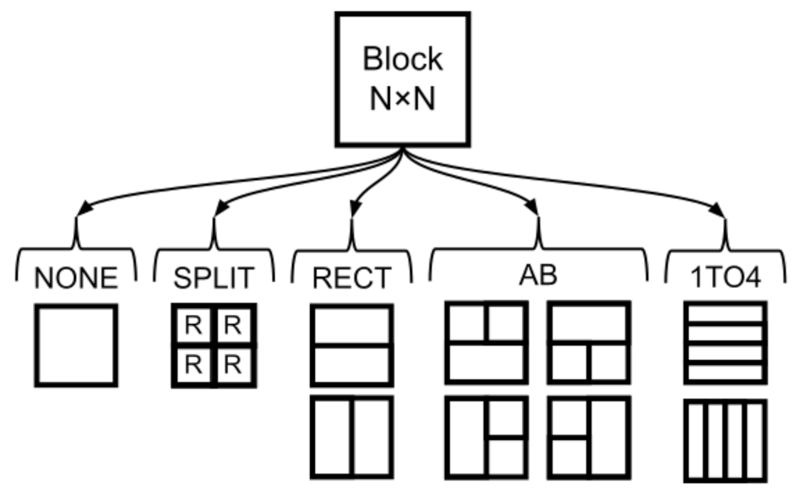
\includegraphics[width=0.5\textwidth]{FIGURES/fig_14.png}
    \caption{Tipos de particionamentos permitidos no formato AV1. Fonte: Elaborada pelo autor.}
    \label{fig:14}
\end{figure}

Dessa forma, é possível calcular o número total de arranjos de árvores existentes para cada superbloco do AV1, que é de 2.555 combinações. Detalhamos o cálculo desse número no Apêndice \ref{apx:B}. Considerando o rol de ferramentas disponíveis para realizar as predições intraquadro ou interquadros no AV1, para todas essas 2.555 combinações, em uma implementação de busca exaustiva, é possível afirmar que a aplicabilidade desse processo de codificação de vídeo seria inviável sem o uso de algum acelerador de hardware dedicado para esse fim. Por essa razão, o software referência do AV1, mesmo em suas versões iniciais, não utiliza algoritmos de busca exaustiva em seus fluxos de execução, optando por condicionais de paradas antecipadas (podas) que permitem a interrupção dos testes. Até a publicação da versão 2.0 do software de referência do AV1 (\textit{libaom}), as podas eram realizadas por técnicas baseadas em análises estatísticas. Desde então, as novas versões do software de referência utilizam modelos de aprendizado de máquina para predizer as podas, conforme descrito em \citet{bib:av1_ml_partitioning}.

Dessa forma, duas análises distintas precisam ser feitas sobre o AV1. A primeira sobre o custo computacional da execução do codificador de referência do AV1 sob diferentes estruturas de particionamento (seção \ref{cap:5.1}) e a segunda sobre a distribuição de ocorrências da subdivisão dos blocos em quatro novos ramos (modo SPLIT) na árvore de particionamentos (seção \ref{cap:5.2}).

\section{Complexidade das Estruturas de Particionamento}
\label{cap:5.1}

Para avaliar o custo computacional do processo de particionamento de blocos do formato AV1, realizou-se uma série de experimentos. Para a realização desses experimentos, foi utilizada a versão do \textit{libaom} disponível no momento inicial da pesquisa apresentada nesta tese (v1.0.0). Note-se que esta versão é diferente da utilizada nas etapas finais da pesquisa apresentada nesta tese, que é mais atualizada (como vimos na seção \ref{cap:4.2}). Apesar da versão 3.5.0 ser 61\% mais rápida que a versão 1.0.0 e apresentar um aumento de 4,07\% de BD-rate, conforme experimentos próprios realizados com cinco vídeos HD1080, as proporções gerais de complexidade observadas neste capítulo tendem a se manter.

O experimento realizado consiste em ativar e desativar ferramentas do \textit{libaom}, em uma estratégia conhecida como \textit{tool-on/off analysis}. Como o objetivo consiste em analisar as estruturas de particionamento, focamos em avaliar os parâmetros do \textit{libaom} que permitem a manipulação da árvore de particionamento. Assim, foi possível definir as 18 variações de parâmetros descritas na Tabela \ref{tab:VIII}. Podem ser observadas diversas variações, como ativar ou desativar os tipos \textit{RECT}, \textit{AB} e \textit{1TO4} (respectivamente, os parâmetros \texttt{enable-rect-partitions}, \texttt{enable-ab-partitions} e \texttt{enable-1to4-partitions}) ou realizar alterações diretas nas profundidades da árvore de particionamentos do AV1, através do tamanho de bloco quadrático máximo (\texttt{max-partition-size}) e mínimo (\texttt{min-partition-size}) permitidos. Neste último caso, existe uma restrição crítica: o valor mínimo do tamanho quadrático deve ser sempre menor que o valor máximo. Na Tabela \ref{tab:VIII}, também é apresentado o total de combinações de árvores que o AV1 poderá dispor para testes (considerando o algoritmo descrito no Apêndice \ref{apx:B}).

\afterpage{
\clearpage

\begin{landscape}
{\footnotesize
\begin{longtblr}[
    caption = {Experimentos de \textit{tool-on/off analysis} das árvores de particionamento do \textit{libaom}.},
    label = {tab:VIII}
]{
    colspec = {c|l|c|r|r|r},
    rowhead = 1,
    hlines,
    row{even} = {gray9}
}
\hline
\textbf{Combinação} & \textbf{Parâmetro} & \textbf{Arranjos Máximos de Árvores} & \textbf{BD-rate (\%)} & \textbf{TS (\%)} & \textbf{Razão}\\

0 & Referência & 2555 & \SetCell[c=1]{c}-~- & \SetCell[c=1]{c}-~- & \SetCell[c=1]{c}-~-\\
1 & -~-enable-rect-partitions=0 & 1365 & 4,81 & 36,22 & 0,133\\
2 & -~-enable-ab-partitions=0 & 2215 & 0,39 & 12,88 & 0,030\\
3 & -~-enable-1to4-partitions=0 & 2387 & 0,33 & 13,20 & 0,025\\
4 & -~-sb-size=64 & 2548 & 0,49 & 15,49 & 0,032\\
5 & -~-min-partition-size=64 -~-max-partition-size=128 & 43 & 92,68 & 65,75 & 1,409\\
6 & -~-min-partition-size=32 -~-max-partition-size=128 & 187 & 30,17 & 39,81 & 0,758\\
7 & -~-min-partition-size=16 -~-max-partition-size=128 & 763 & 8,03 & 24,13 & 0,333\\
8 & -~-min-partition-size=8 -~-max-partition-size=128 & 1531 & 0,45 & 14,15 & 0,032\\
9 & -~-min-partition-size=32 -~-max-partition-size=64 & 180 & 30,65 & 53,57 & 0,572\\
10 & -~-min-partition-size=16 -~-max-partition-size=64 & 756 & 8,57 & 35,49 & 0,241\\
11 & -~-min-partition-size=8 -~-max-partition-size=64 & 1524 & 0,95 & 20,13 & 0,047\\
12 & -~-min-partition-size=4 -~-max-partition-size=64 & 2548 & 0,48 & 17,40 & 0,027\\
13 & -~-min-partition-size=16 -~-max-partition-size=32 & 720 & 14,27 & 49,58 & 0,288\\
14 & -~-min-partition-size=8 -~-max-partition-size=32 & 1488 & 6,49 & 36,39 & 0,178\\
15 & -~-min-partition-size=4 -~-max-partition-size=32 & 2512 & 6,06 & 33,61 & 0,180\\
16 & -~-min-partition-size=8 -~-max-partition-size=16 & 1344 & 28,90 & 60,31 & 0,479\\
17 & -~-min-partition-size=4 -~-max-partition-size=16 & 2368 & 28,35 & 55,80 & 0,508\\
18 & -~-min-partition-size=4 -~-max-partition-size=8 & 1792 & 103,56 & 76,66 & 1,351\\
\hline
\end{longtblr}
}
\end{landscape}
}


Foram realizados, portanto, 19 experimentos, os 18 experimentos descritos na Tabela \ref{tab:VIII}, além da codificação de referência (00) usada como base para as comparações. Todas essas codificações utilizam as mesmas configurações padrões do \textit{libaom} e utilizam quatro vídeos HD1080, conforme descrição detalhada realizada na seção \ref{cap:4.1}. Mesmo sem executar os experimentos, a Tabela \ref{tab:VIII} permite especular que a combinação 05 (testar apenas as profundidades 0 e 1) tende a ser a mais rápida, por possuir poucos arranjos de árvores para realização de testes preditivos (apenas 43). Em termos de redução de tempo de codificação, a combinação 05 deve ser seguida da combinação 09 (testar apenas as profundidades 1 e 2), pois esta possui 180 variações de árvores. No entanto, apesar de esses dois experimentos possuírem poucas possibilidades de árvores disponíveis para avaliação, as etapas de predições possuem custos de processamento diferentes, a depender do tamanho do bloco, o que influencia no tempo total de codificação. Por outro lado, os experimentos 04 e 12 tendem a apresentar resultados iguais, pois ambos possuem o mesmo número de árvores disponíveis para teste, inclusive com configurações praticamente idênticas. Na Tabela \ref{tab:VIII}, também constam os resultados obtidos com a execução dos experimentos, onde são mostrados valores de BD-rate e TS (vide equação 7).

Como mencionado anteriormente, esperava-se que as combinações 05 e 09 apresentassem os maiores valores de TS de todo o conjunto de experimentos. Todavia, isso não é o que se observa na Tabela \ref{tab:VIII}. As combinações com os maiores valores de TS foram as de número 18, 05 e 16, com a combinação 09 aparecendo apenas em quinto lugar. O maior destaque é para a combinação 18, com uma redução de complexidade de 76,66\%, o que se dá pela sua limitação: o codificador só tem à sua disposição blocos pequenos (8$\times$8 ou menores). Em termos gerais, processar os estágios de predição em blocos pequenos tende a ser computacionalmente menos custoso que em blocos maiores, como é possível observar com os dois extremos apresentados na Tabela \ref{tab:VIII}, onde vemos 43 árvores distintas na combinação 05 frente a 1792 da combinação 18. Outra parte da explicação para o valor de TS elevado da combinação 18, assim como na 16 (60,31\%), se deve ao percentual de representação dos diferentes tamanhos de bloco em um quadro, conforme discutido anteriormente no capítulo \ref{cap:2}. Naquele capítulo, a Tabela \ref{tab:I} evidenciou que um bloco 8$\times$8 representa uma área de 0.00309\% de um quadro de vídeo HD1080, enquanto blocos 4$\times$4 representam uma área ainda menor (0.00077\%). Logo, as perdas ocasionadas por predições imprecisas nesses casos é menor, tanto em termos de qualidade subjetiva, quanto em termos de qualidade objetiva da imagem. No entanto, há um agravante no uso exclusivo desses tamanhos de bloco: o elevado custo em taxa de bits para representação desses blocos no \textit{bitstream} codificado, justificando o BD-rate elevadíssimo observado no experimento 18.

Enquanto a combinação 18 emprega apenas blocos pequenos e isso impacta significativamente no BD-rate, a combinação 05, que utiliza exclusivamente blocos grandes, também apresenta problemas similares. Apesar de a quantidade de bits para representar a existência de blocos grandes ser significativamente menor, os resíduos da predição interquadros (especialmente) tendem a ser maiores, aumentando a complexidade das etapas seguintes à predição, como o cálculo de transformadas, quantização e codificação de entropia. Além disso, qualitativamente, a imagem resultante é menos agradável ao usuário, visto que sofre maiores perdas.

Na Tabela \ref{tab:VIII}, há outros resultados que merecem destaque, como as combinações que evitam particionamentos quaternários (combinação 03), ternários (02) e binários (01). Esta última combinação, inclusive, desabilita automaticamente as combinações 02 e 03. Os três experimentos apresentaram uma redução de tempo de 13,20\%, 12,88\% e 36,22\%, respectivamente. Como a combinação 01 também desabilita os particionamentos ternários e quaternários, é possível estimar que o particionamento binário possui um impacto aproximado de 10\% do tempo total de codificação do \textit{libaom} (ou seja, a subtração entre 36,22\% e os valores de 12,88\% e 13,20\%). Observa-se na Tabela \ref{tab:VIII} um baixo impacto na eficiência de codificação ao se desabilitar os particionamentos ternários (combinação 02) e quaternários (combinação 03) em vídeos HD1080, inferior a 0,4\% em BD-rate. No entanto, apesar dos particionamentos binários exigirem um tempo de codificação pouco abaixo dos particionamentos ternários e quaternários, o experimento com a combinação 01 indica que a ausência de predições retangulares impacta a codificação com um acréscimo de 4,81\% em BD-rate. Em outras palavras, é importante para a boa eficiência do codificador a disponibilidade dos modos de particionamento retangulares.

Outro ponto anteriormente levantado foi a semelhança entre os experimentos 04 e 12, que levam à mesma configuração no codificador. Apesar de ambos tecnicamente disporem do mesmo arranjo de árvores para codificação, essa igualdade não se replica nos resultados de BD-rate, respectivamente de 0,49\% e 0,48\%, e nem de TS, respectivamente de 15,49\% e 17,40\%. O principal fator que leva a essa diferença nos resultados está no fluxo de execução do próprio \textit{libaom}, que será apresentado na seção \ref{cap:7.4}. Enquanto no experimento 04 o \textit{libaom} parte de um superbloco de 64$\times$64 amostras, iniciando suas variáveis de controle a partir desse tamanho de bloco, a codificação com limitações na árvore (experimento 12) não impede que as variáveis do superbloco sejam iniciadas no bloco quadrático de tamanho 128$\times$128. Consequentemente, o \textit{libaom} dispõe de mais informações para melhor tomada de decisão no segundo caso, o que explica os melhores resultados do experimento 12 em relação ao experimento 04. 

\section{Distribuição de Profundidades e do Modo \textit{SPLIT}}
\label{cap:5.2}

Outro experimento relevante para o desenvolvimento das soluções apresentadas nos capítulos seguintes desta tese é a avaliação da distribuição de profundidades e do uso do modo \textit{SPLIT} na codificação de vídeo segundo o formato AV1. Conhecer quais profundidades tendem a ter maior relevância para a codificação auxilia-nos a considerá-las prioritárias nas tomadas de decisão, principalmente no que se refere ao processo de busca preditiva, seja intraquadro ou interquadros. Também é importante saber a distribuição da utilização do modo \textit{SPLIT} ao longo das profundidades da árvore de particionamento do AV1, pois ela evidencia quais profundidades tendem a ser mais particionadas. Dessa forma, com esses dois dados extras, torna-se possível identificar quais profundidades são mais ou menos interessantes de serem consideradas durante o desenvolvimento de uma solução para codificação ou transcodificação rápida.

Diferentemente do experimento apresentado na seção anterior, a avaliação relatada nesta seção leva em consideração várias decisões tomadas em fases posteriores da tese. Portanto, os resultados apresentados aqui foram obtidos com uma versão atualizada do software de referência do AV1 e consideram 14 sequências de vídeo HD1080 (conforme detalhado na seção \ref{cap:4.1}).

A Figura \ref{fig:16} representa a distribuição das ocorrências de cada uma das profundidades permitidas no formato AV1, considerando os quatro níveis de quantização (vide seção \ref{cap:4.2}) utilizados nos experimentos relatados ao longo desta tese. A Figura \ref{fig:16} foi gerada através de uma comparação da média das áreas de ocorrência de cada uma das profundidades em relação à área total do quadro codificado. Desta forma, é possível observar uma maior utilização da profundidade 1 (bloco quadrático de tamanho 64$\times$64 pixels), exceto quando o CQ é igual a 20, onde há uma opção pela profundidade 2. Em outras palavras, essa observação nos dá indícios de que o codificador AV1 tende a optar pela utilização dos blocos de altura ou largura igual a 64, em algum dos nove tipos de particionamentos disponíveis. Logo, considerando os experimentos realizados na seção anterior, compreende-se a causa do elevado impacto negativo das combinações 13 e 18 ao omitir a disponibilidade dos blocos 64$\times$64. Os experimentos mostram que não permitir o uso dessa profundidade implica, invariavelmente, na distribuição dos blocos em profundidades menores, o que causa um aumento na taxa de bits necessária para representar o vídeo codificado.

\begin{figure}
    \centering
    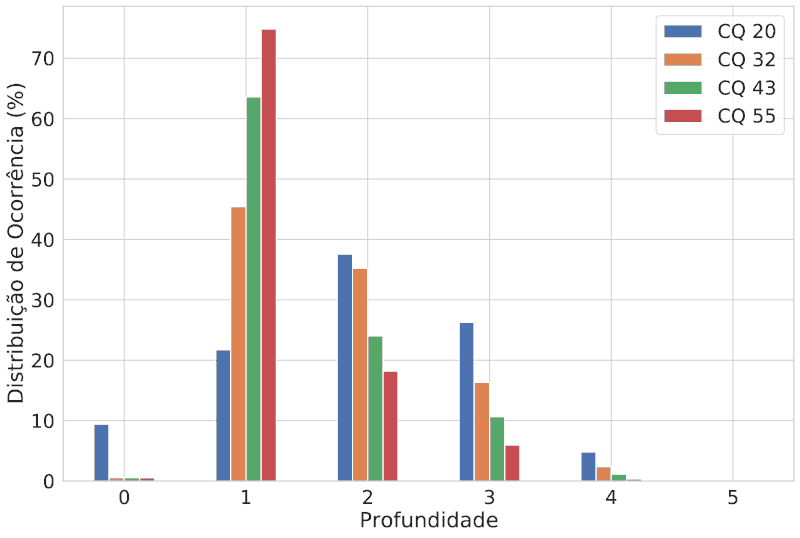
\includegraphics[width=0.75\textwidth]{FIGURES/fig_16.png}
    \caption{Média de distribuição das profundidades da árvore de particionamento do AV1. Fonte: Elaborada pelo autor.}
    \label{fig:16}
\end{figure}

Outra constatação a partir da Figura \ref{fig:16} é a relativa ausência de blocos 4$\times$4, que representam uma área média inferior a 0,3\% dos vídeos HD1080 utilizados nos experimentos. O mesmo pode ser observado com a profundidade 0, que ocupa uma área média inferior a 1\% em quase todos os experimentos realizados com diferentes níveis de quantização, exceto no caso da quantização configurada com CQ 20, onde a área de emprego da profundidade 0 é de 9\%. Essa observação contraria a expectativa de que vídeos codificados com menores parâmetros de quantização tendem a apresentar mais particionamentos; os resultados mostram que neste caso foram utilizados blocos maiores na codificação.

Em complemento à análise de distribuição de profundidades, é importante avaliar também o índice de utilização do modo de particionamento \textit{SPLIT} para cada profundidade da árvore. Essa informação é particularmente útil para definir quais profundidades são mais utilizadas e, consequentemente, quais são os particionamentos que, caso forçados ou evitados, têm potencial de causar maior impacto na eficiência de codificação do software do AV1. Utilizando os mesmos vídeos do experimento apresentado na Figura \ref{fig:16}, a Figura \ref{fig:17} mostra a taxa de uso do modo \textit{SPLIT} para cada profundidade e para cada nível de quantização considerado nos experimentos apresentados nesta tese. Na Figura \ref{fig:17}, os dados estão distribuídos de acordo com duas escolhas: o codificador decidiu pelo bloco naquele nível de profundidade (não-\textit{SPLIT}, em laranja) ou decidiu por subparticionar o bloco (\textit{SPLIT}, em azul). Em cada profundidade considerada (eixo x) o somatório de casos \textit{SPLIT} e não-\textit{SPLIT} é igual ao total de casos \textit{SPLIT} da profundidade anterior. No topo de cada coluna, encontra-se destacado o valor proporcional do modo \textit{SPLIT} (em azul) para aquela profundidade. Desta forma, torna-se possível identificar a probabilidade de ocorrência de particionamentos em cada profundidade e, ao mesmo tempo, identificar quais profundidades são utilizadas, complementando a Figura \ref{fig:16}. Por exemplo, na profundidade 2 (blocos 32$\times$32), considerando uma codificação com CQ 20, o codificador \textit{libaom} opta por subparticionar o bloco em blocos menores em 45,46\% das vezes. Quando processa blocos em profundidade 4, considerando o mesmo CQ 20, em apenas 4,11\% das vezes o codificador opta por subparticionar em blocos menores na profundidade 5.

\begin{figure}
    \centering
    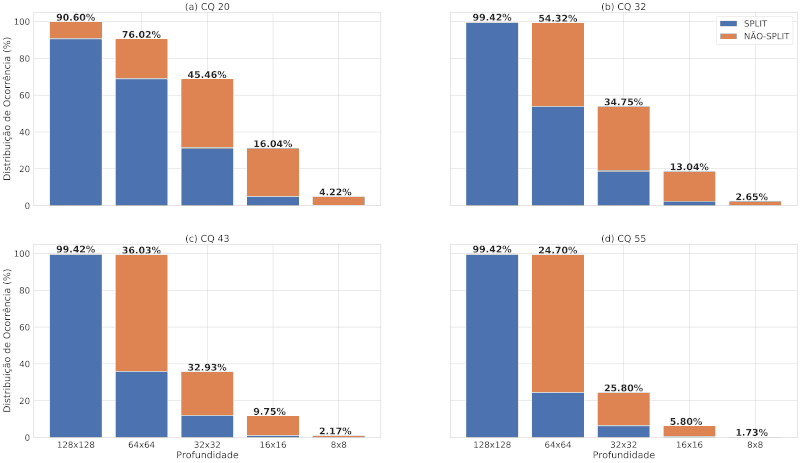
\includegraphics[width=\textwidth]{FIGURES/fig_17.png}
    \caption{Probabilidade do subparticionamento em modo \textit{SPLIT} para cada nível da árvore de particionamento do AV1, em CQs (a) 20, (b) 32, (c) 43 e (d) 55. Fonte: Elaborada pelo autor.}
    \label{fig:17}
\end{figure}

Evidenciamos neste capítulo que a escolha de particionamentos e de tamanhos de blocos influencia consideravelmente o custo computacional do software de referência do AV1 e também a sua eficiência de codificação. Portanto, uma das tarefas essenciais de um codificador ou transcodificador rápido, quando baseado em escolhas de particionamentos, é identificar a melhor combinação de blocos sem a necessidade de realizar um grande número de testes. Nesse sentido, o capítulo \ref{cap:6} contempla as primeiras soluções desenvolvidas no escopo desta tese, que envolvem transcodificadores rápidos por heurísticas baseados em análises estatísticas. No capítulo \ref{cap:7}, apresentamos a proposta de transcodificador rápido baseado no reaproveitamento de estruturas de particionamento com uso de modelos preditivos gerados por algoritmos de aprendizado de máquina, aplicados a diversos transcodificadores.

\chapter{Transcodificação de Vídeo Baseado em Heurísticas}
\label{cap:6}

Este capítulo apresenta as primeiras soluções desenvolvidas no escopo desta tese para acelerar o transcodificador de H.265/HEVC para AV1 e de VP9 para AV1, inclusive ambos já foram publicados em \cite{bib:borges2_2021} e \cite{bib:borges_2021}. Apesar de não envolverem uso de aprendizado de máquina, foram desenvolvidas como passos iniciais necessários para a concepção das soluções seguintes apresentadas nesta tese. Além disso, as soluções foram utilizadas como base de comparação com aquelas baseadas em aprendizado de máquina, conforme apresentaremos no capítulo \ref{cap:7}.

\section{Transcodificador H.265/HEVC para AV1}
\label{cap:6.1}

A primeira solução desenvolvida no escopo desta tese consiste em um transcodificador H.265/HEVC para AV1 que utiliza informações de profundidade de blocos observados durante a decodificação, a fim de inferir sobre quais níveis de profundidade a árvore de particionamento do AV1 poderá realizar as buscas preditivas, seja intraquadro ou interquadros. Para tanto, avalia-se as profundidades observadas durante a decodificação do vídeo em H.265/HEVC e determina-se um subconjunto de profundidades ao AV1, cujas profundidades são próximas ao observado no decodificador. 

Na Tabela \ref{tab:V} mostramos que há vários tamanhos de blocos similares entre os vários formatos de codificação de vídeo. Também já mencionamos que há diversas formas de se organizar uma estrutura de particionamento de blocos. Por exemplo, no capítulo \ref{cap:5}, relatamos que o AV1 utiliza uma estrutura baseada em árvores, sendo a raiz um superbloco de tamanho 128$\times$128. No entanto, a estrutura principal do H.265/HEVC divide o quadro em áreas de 64$\times$64 amostras, denominadas \textit{Coding Tree Units} (CTU), conforme pode ser visto em \citet{bib:hevc}. Cada CTU é dividida em uma série de \textit{Coding Units} (CU). A CU é a responsável por particionar a CTU em diferentes profundidades, todas elas de tamanho quadrático, partindo de 64$\times$64 até 8$\times$8 amostras. De cada CU partem duas outras estruturas: a \textit{Prediction Unit} (PU) e a \textit{Transform Unit} (TU). A primeira é responsável por definir um arranjo de blocos a ser utilizado pelas etapas de predição, podendo assumir formas simétricas (2N$\times$2N, N$\times$2N, 2N$\times$N e N$\times$N) ou assimétricas (2N$\times$nU, 2N$\times$nD, nL$\times$2N e nR$\times$2N), como representado na Figura \ref{fig:18}. Por fim, a TU é responsável por dividir a CU em áreas quadráticas a fim de processar os resíduos gerados após as predições na etapa de transformadas. A TU pode assumir tamanhos quadráticos que variam de 32$\times$32 até 4$\times$4, desde que não ultrapasse até dois tamanhos de blocos menores que o observado na CU. Diferentemente do AV1, onde cada elemento está presente em um ramo próprio da árvore de particionamentos, no H.265/HEVC cada CTU, CU e TU seguem o padrão \textit{Raster-Scan} \cite{bib:raster} de posicionamentos de blocos, onde cada elemento é posicionado da esquerda para a direita e de cima para baixo, respeitando os limites estabelecidos por outras estruturas de mesmo tipo. 

\begin{figure}
    \centering
    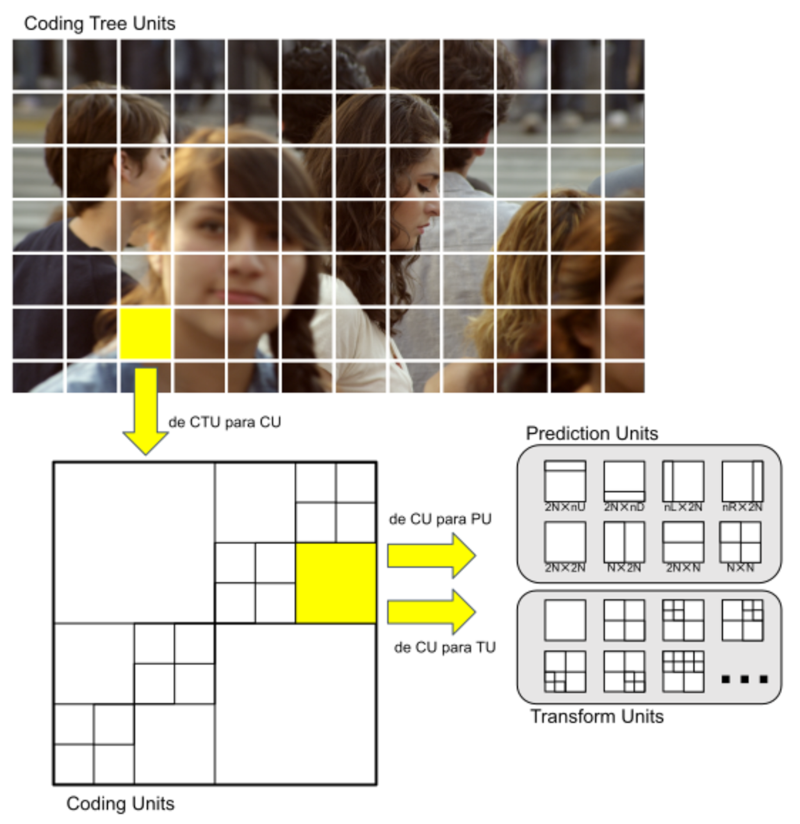
\includegraphics[width=0.85\textwidth]{FIGURES/fig_18.png}
    \caption{Exemplo de particionamento de uma CTU do H.265/HEVC. Fonte: Elaborada pelo autor.}
    \label{fig:18}
\end{figure}

No entanto, dentre todas essas estruturas de particionamento disponíveis no H.265/HEVC, é a CU que mais interessa a solução aqui apresentada, pois é essa estrutura que possibilita a identificação das regiões de agrupamento de pixels e, consequentemente, semelhante a profundidade de uma árvore de particionamento. Dessa forma, foi realizada uma avaliação de correlação entre os tamanhos de blocos observados na CU do H.265/HEVC, convertidos em profundidades com valores iguais ao do AV1, e das profundidades da árvore de particionamento do AV1. Essa avaliação está resumida na Figura \ref{fig:19}, na qual quanto mais intenso a cor, maior é a correlação entre as profundidades observadas. Logo, observa-se que quando o H.265/HEVC opta por algum tamanho de CU, os tamanhos de blocos observados no codificador AV1 tendem a serem iguais (diagonal destacada). Por exemplo, ao notar-se, durante a decodificação, a utilização da CU de tamanho 32$\times$32 (convertido para profundidade 2), em 58,09\% das vezes o codificador AV1, durante a transcodificação, também irá optar por algum arranjo de particionamentos na profundidade 2. Mas existe algumas vezes (19,21\%) em que o AV1 decide expandir a árvore de particionamentos para uma profundidade maior (de nível 3). Em raras exceções, quando o H.265/HEVC utiliza uma CU de 32$\times$32 (profundidade 2), o AV1 decide utilizar blocos de 4$\times$4 (profundidade 5), mais explicitamente, em 0,18\% das vezes. Desta forma, cada linha da Figura \ref{fig:19} representa todas as probabilidades de escolha por parte do AV1, para cada profundidade observada no decodificador H.265/HEVC.

\begin{figure}
    \centering
    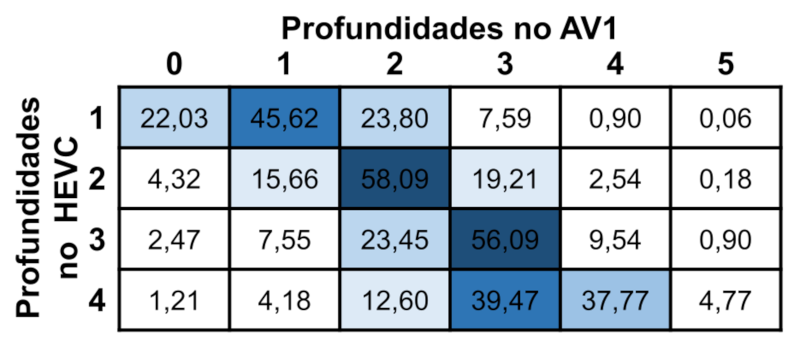
\includegraphics[width=0.75\textwidth]{FIGURES/fig_19.png}
    \caption{Correlação entre a profundidade observada na decodificação H.265/HEVC (sob QP 22) e na recodificação do mesmo vídeo para o formato AV1 (sob CQ 20). Fonte: Elaborada pelo autor.}
    \label{fig:19}
\end{figure}

Identificando-se uma correlação entre as profundidades observadas durante a decodificação e a profundidade escolhida no codificador, durante uma transcodificação, hipotetizamos que é possível inferir nas melhores profundidades a serem melhor exploradas preditivamente pelo codificador do AV1. No entanto, como vimos na Figura \ref{fig:19} e ressaltado no parágrafo anterior, todas as profundidades podem ser escolhidas pelo AV1, independentemente da profundidade observada no decodificador H.265/HEVC. Logo, propõe-se um transcodificador que considere profundidades a mais ou a menos ao observado durante a decodificação, a fim de obter transcodificadores rápidos de acordo com as necessidades de quem transcodifica os vídeos.

\subsection{Metodologia}
\label{cap:6.1.1}

Considerando o tamanho de CU observado no decodificador H.265/HEVC, cujo valor é convertido para profundidades de 1 (CU igual a 64$\times$64) até 4 (CU igual a 8$\times$8), a estratégia baseia-se em inferir as profundidades permitidas para exploração na codificação AV1. Essa profundidade observada denominaremos de $DLmap$. Como apresentamos na Figura \ref{fig:19}, na estratégia proposta o codificador AV1 pode optar por utilizar profundidades maiores que o observado em $DLmap$ ou por profundidades menores que o observado em $DLmap$. Em outras palavras, o codificador AV1 poderá optar por qualquer nível de profundidade que esteja algum nível acima ao observado em $DLmap$ (denominada como $La$, do inglês \textit{Levels Above}) ou que esteja níveis abaixo ao observado no $DLmap$ (denominado como $Lb$, do inglês, \textit{Levels Below}). Logo, a profundidade escolhida pelo codificador AV1 (denominada como $DLn$) será algum valor entre $DLmap - La$ e $DLmap + Lb$, para quaisquer valores de $La$ e $Lb$ que estejam entre 0 e 4.

A proposta desta solução é, portanto, averiguar o quão estreita pode ser a faixa de valores $La$ e $Lb$, de forma a permitir uma transcodificação rápida de H.265/HEVC para AV1. Os valores permitidos para as variáveis $La$ e $Lb$ são os mesmos: 0, 1, 2, 3 e 4. O valor 0 obriga que o codificador utilize a profundidade superior ($La$) ou a profundidade inferior ($Lb$) igual à observada na decodificação ($DLmap$); já o valor 4 indica que nenhum limite será imposto. Há, dessa forma, várias combinações de valores de $La$ e $Lb$ – mais precisamente, 25 combinações. Para identificar cada uma dessas combinações, utilizaremos a definição $La$:$Lb$, conforme a Equação \ref{eq:8}:

\begin{equation}
    \label{eq:8}
    La:Lb = \{ DLmap - La \leq DLn \leq DLmap + Lb | La, Lb \in \{ 0, 1, 2, 3, 4 \} \}
\end{equation}

Para exemplificar, consideremos um $La$:$Lb$ igual a 2:3. Então, ao observar no decodificador o uso da CU de tamanho 16$\times$16 ($DLmap$ = 3), isso significa que o codificador, naquela área do vídeo, poderá considerar realizar as predições intraquadro ou interquadros para qualquer tamanho de bloco que esteja dentro da profundidade 1 ($DLmap - La$ = 3 - 2) até a profundidade 6 ($DLmap + Lb$ = 3 + 3). Contudo, como não existe profundidade 6 no AV1, o codificador não sofrerá intervenções para exploração de profundidades além do $DLmap$. É possível observar que algo similar pode acontecer com o limite $DLmap - La$: caso La seja maior que $DLmap$, o limite retornado será negativo. Neste caso, não haverá qualquer interferência no limite superior da árvore de particionamentos

Ao assumir os limites $La$:$Lb$ estabelecidos no parágrafo anterior, é possível estimar o percentual de correlação a ser atingida por cada uma das combinações de $La$:$Lb$, com base nos valores da Figura \ref{fig:19}. Esse percentual de correlações estimadas pode ser visto na Tabela \ref{tab:IX}, onde podemos ver que a combinação 4:4, que é a mais permissiva, não se diferencia de uma transcodificação original (sem restrições). Já a transcodificação mais restritiva (combinação 0:0), tende a apresentar 49,39\% das mesmas profundidades observadas na transcodificação original. Olhando para todos os valores da Tabela \ref{tab:IX}, podemos ver que restringir o limite superior da árvore de particionamentos para $DLmap$, ou seja, $La$=0, faz com que em nenhuma combinação de $La$:$Lb$ atinja-se algum percentual de correlação acima dos 67\%. Em outras palavras, em aproximadamente um terço das profundidades que o transcodificador rápido escolher usar, haverá divergência das profundidades observadas na transcodificação original (sem restrições), caso não seja permitida alguma flexibilidade para considerar profundidades menores que aquelas observadas na decodificação.

\begin{table}
\begin{center}
\caption{Correlação (em porcentagem) estimada com diferentes combinações de $La$ e $Lb$.}
\label{tab:IX}
\footnotesize

\begin{tblr}{
 colspec = {r|r|r|r|r|r|r},
 hlines,
 row{even} = {gray9}
}
\hline
\SetCell[c=2,r=2]{} && \SetCell[c=5]{c}\textbf{Níveis Acima (La)} \\
 && 0 & 1 & 2 & 3 & 4 \\
\SetCell[r=5]{c} \textbf{Níveis Abaixo (Lb)} & 0 & 49,39 & 74,55 & 80,66 & 82,33 & 82,63 \\
 & 1 & 63,72 & 88,88 & 94,99 & 96,66 & 96,96 \\
 & 2 & 66,48 & 91,63 & 97,75 & 99,41 & 99,72 \\
 & 3 & 66,75 & 91,9 & 98,02 & 99,68 & 99,99 \\
 & 4 & 66,77 & 91,92 & 98,04 & 99,7 & 100,00 \\
\hline
\end{tblr}
\end{center}
\end{table}


Para possibilitar a aplicação dos limites La:Lb, expressos na Equação \ref{eq:8}, de forma a possibilitar ao codificador que seja encontrada a melhor profundidade ($DLn$ final) de forma rápida, propusemos o algoritmo exemplificado no fluxograma da Figura \ref{fig:20}. Nesta figura, é possível identificar três pontos de convergência:

\begin{enumerate} [1.]
    \item Caso o $DLn$ atual seja menor que o limite superior ($DLmap - La$), aplica-se o subparticionamento do bloco. No entanto, o modo simples da predição intraquadro e interquadros deve ser aplicado;
    
    \item Caso o $DLn$ atual seja maior que o limite inferior ($DLmap + Lb$), proíbe-se o subparticionamento do bloco e encerra-se o fluxo de particionamentos;

    \item Caso os limites superiores ou inferiores estejam fora dos limites de profundidade existentes, ignora-se a limitação
    
\end{enumerate}

\begin{figure}
    \centering
    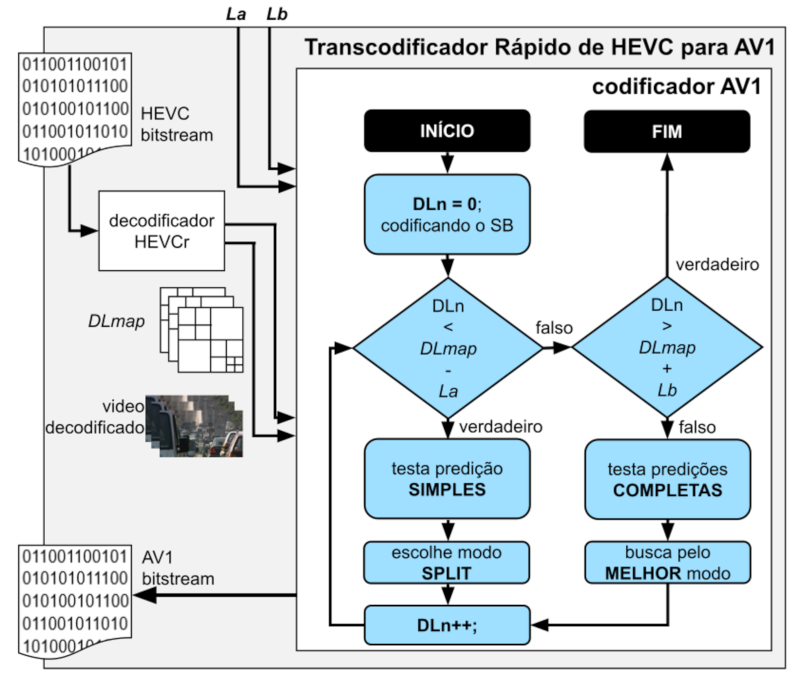
\includegraphics[width=0.75\textwidth]{FIGURES/fig_20.png}
    \caption{Fluxograma da proposta de transcodificador rápido de vídeo de H.265/HEVC para AV1 baseado em heurísticas. Fonte: Elaborada pelo autor.}
    \label{fig:20}
\end{figure}

Observe que, caso o primeiro condicional, apresentado na Figura \ref{fig:20}, seja verdadeiro, identificamos a obrigatoriedade de o codificador AV1 realizar ao menos um único modo de predição, o qual denominamos de modo simples. O modo simples da predição intraquadro é o modo \texttt{DC} e o modo simples da predição interquadros é o  modo \texttt{NEARESTMV}, estes modos foram escolhidos por serem os primeiros modos a serem testados nestas etapas de predição.  Essa predição obrigatória serve como garantia de que o valor obtido durante o cálculo do custo taxa-distorção (do inglês, \textit{rate-distortion cost}, ou rd-cost) seja corretamente gerado, principalmente após os subparticionamentos de blocos. Isso é necessário, pois é através do cálculo de rd-cost que o codificador identifica quais combinação de árvores de profundidades e seus respectivos modos preditivos são melhores para serem aplicados em um determinado momento da codificação, para um determinado conteúdo. No entanto, se aplicarmos diretamente o subparticionamento dos primeiros níveis de profundidade da árvore sem a obtenção de qualquer valor de rd-cost, o codificador não estará apto a decidir se aquela combinação de árvore e de modos preditivos é melhor ou pior que outra, podendo entrar em uma situação impossível (por exemplo, uma repetição infinita).

\subsection{Resultados}
\label{cap:6.1.2}

Para verificar a eficiência da proposta de transcodificador rápido, os primeiros 60 quadros de quatro sequências de vídeos HD1080 foram utilizados para realização do experimento, utilizando a versão 1.0.0 do software de referência do codificador AV1. Os resultados deste experimento podem ser vistos na Tabela \ref{tab:X}, onde todas as combinações de La:Lb estão ordenadas por redução do tempo de transcodificação (TS). De forma geral, é possível observar que existe uma tendência de aumento proporcional entre o TS e o BD-rate, principalmente quando há uma maior restrição entre os valores de $La$ e de $Lb$, o que é facilmente explicável, já que se reduz significativamente a quantidade de blocos disponíveis para testes. 

Como esperado, a combinação mais permissiva (4:4) não se diferencia da transcodificação sem intervenções e, por outro lado, a combinação mais restritiva (0:0) apresenta maior TS e, consequentemente, maior BD-rate. Já a combinação 2:2, intermediária entre essas duas, é discreta em seus resultados, acelerando apenas 5\% a um custo de reduzir a eficiência de codificação em 0,1145\%. O único caso que apresentou resultados fora do esperado é a combinação 3:4, cujo tempo de transcodificação rápido pode ser considerado uma variação normal de execução do software, com 0,20\% em relação à transcodificação original. Contudo, essa combinação apresentou um BD-rate negativo (de -0,0128\%), ou seja, mostrou-se mais eficiente em codificar o vídeo decodificado que a versão de codificação de referência. Analisando-se os dados brutos, identificou-se que a combinação 3:4 apresentou bons resultados em sequências de menor variação de movimento, onde os vídeos possuem mais movimento de câmera do que de objetos.

\begin{table}
\begin{center}
\caption{Resultados das transcodificações H,265/HEVC para AV1 sob diferentes combinações de $La:Lb$.}
\label{tab:X}
\footnotesize

\begin{tblr}{
    colspec = {c|r|r|r},
    hlines,
    row{even} = {gray9}
}
\hline
\textbf{$La:Lb$} & \textbf{BD-rate (\%)} & \textbf{TS (\%)} & \textbf{Razão} \\
0:0 & 14,6688 & 61,20 & 0,240 \\
2:0 & 5,0935 & 40,80 & 0,125 \\
3:0 & 5,0628 & 40,70 & 0,124 \\
4:0 & 5,0215 & 40,00 & 0,126 \\
1:0 & 6,1817 & 39,80 & 0,155 \\
0:1 & 6,1688 & 32,00 & 0,193 \\
1:1 & 1,1950 & 21,00 & 0,057 \\
0:2 & 3,9088 & 20,00 & 0,195 \\
2:1 & 0,8708 & 18,00 & 0,048 \\
3:1 & 0,8703 & 17,70 & 0,049 \\
4:1 & 0,9020 & 17,70 & 0,051 \\
0:3 & 3,5850 & 15,40 & 0,233 \\
0:4 & 3,5125 & 15,10 & 0,233 \\
1:2 & 0,4263 & 8,00 & 0,053 \\
2:2 & 0,1145 & 5,00 & 0,023 \\
3:2 & 0,0645 & 4,60 & 0,014 \\
4:2 & 0,0583 & 4,60 & 0,013 \\
1:4 & 0,3180 & 3,50 & 0,091 \\
1:3 & 0,3308 & 3,50 & 0,094 \\
2:3 & 0,0070 & 0,50 & 0,014 \\
3:3 & 0,0043 & 0,40 & 0,011 \\
2:4 & 0,0050 & 0,30 & 0,017 \\
4:3 & 0,0493 & 0,30 & 0,164 \\
3:4 & -0,0128 & 0,20 & -0,064 \\
4:4 & 0,0000 & 0,00 & \SetCell[c=1]{c}-~- \\
\hline
\end{tblr}
\end{center}
\end{table}


A relação existente entre o TS atingido e o impacto no BD-rate, na Tabela \ref{tab:X}, pode ser observado através da coluna Razão. Conforme já foi apresentado no capítulo \ref{cap:3}, Razão indica o acréscimo de BD-rate para cada percentual de tempo acelerado. Portanto, quanto menor esse valor, melhor tende a ser a solução proposta para transcodificação rápida. Observando apenas o valor de Razão, a melhor combinação (exceto a 3:4) é a 3:3, que impacta em 0,011\% de BD-rate para cada percentual de tempo reduzido. Todavia, essa combinação tem potencial de aceleração inferior a 0,5\% do tempo de transcodificação original, ou seja, também pode ser considerada uma variação normal da execução do software. Considerando os resultados de TS superiores a 5\%, a combinação 2:2 é a melhor, com um aumento de 0,023\% de BD-rate para cada percentual de tempo reduzido. Nota-se, inclusive, que todas as combinações com $Lb$ igual ou superior a 2 atingem menos de 10\% de aceleração. Ou seja, autorizar que o \textit{libaom} considere blocos de um nível de profundidade muito além do observado na decodificação não traz ganhos significativos de tempo. Por outro lado, permitir apenas uma única profundidade além do observado ($Lb$=1) possibilita atingir TS moderados (entre 10\% e 20\%). Já ganhos significativos de TS (30\% ou mais) se apresentam somente quando não se permite testar nenhuma profundidade além daquela observada ($Lb$=0). Essas três observações pontuais são relevantes para a definição da metodologia de transcodificação rápida com uso de aprendizado de máquina (capítulo \ref{cap:7}).

O único trabalho disponível para comparação com a nossa proposta de transcodificador rápido de H.265/HEVC para AV1 foi desenvolvido por \citet{bib:chen_2019}, que propôs duas abordagens em seu trabalho. Na primeira abordagem, o autor limita as profundidades máximas e mínimas da árvore de particionamento do codificador AV1 com base no histórico de profundidades observadas na decodificação HEVC. Basicamente, o autor aplica, quadro a quadro, uma análise probabilística de ocorrência de cada uma das profundidades observadas anteriormente, considerando pesos menores a quadros mais distantes ao quadro atual em codificação. Assim, obtém uma estimativa de quais profundidades não precisam ser consideradas na avaliação do codificador AV1. Ainda nessa primeira abordagem, caso a profundidade seja superior ao limite estimado no trabalho, o autor desabilita os testes de predição interquadros com particionamentos não-quadráticos. Já na segunda abordagem, \citet{bib:chen_2019} utiliza um modelo de inferência bayesiana condicional \cite{bib:bayesian_ref} para identificar o fim do particionamento de blocos. Segundo \citet{bib:chen_2019}, essa segunda abordagem foi inspirada no trabalho de \cite{bib:guo2_2018}, que utilizou um modelo de inferência bayesiana condicional para reduzir a complexidade do processo de particionamento do codificador AV1, ainda em suas versões iniciais (pré v1.0.0). Dessa forma, \citet{bib:chen_2019} obtém uma aceleração de 37,8\% da transcodificação a um custo de elevar o BD-rate em apenas 0,79\%, conforme já apresentamos na seção \ref{cap:3.1}. Logo, apesar da primeira abordagem do autor ser similar à nossa, a forma como se dá a análise estatística é diferente. Enquanto \citet{bib:chen_2019} realiza uma análise estatística local, quadro a quadro e em tempo de execução, a nossa proposta considera uma análise estatística de vídeos inteiros e diferentes ao que se está codificando no momento. Ainda assim, os resultados apresentados por \citet{bib:chen_2019} se assemelham à nossa combinação 2:2 (0,1145\% de BD-rate e 5,00\% de TS) ou à combinação 2:4 (0,0050 de BD-rate e 0,30\% de TS), pois \citet{bib:chen_2019} apresenta uma Razão de 0,0020\% de BD-rate para cada porcento de redução de tempo. Todavia, apesar de proporcionalmente \citet{bib:chen_2019} apresentar valores similares aos nossos, o autor obtém um TS superior.

\subsection{Ajuste de Complexidade Experimental}
\label{cap:6.1.3}

Por fim, considerando os resultados apresentados no transcodificador de H.265/HEVC para AV1, baseado em permissões de profundidade máxima ($La$) e mínima ($Lb$) da árvore de particionamentos, demonstrados na subseção anterior, avaliamos também um cenário de ajuste de complexidade em tempo de codificação. A ideia principal consiste em  disponibilizar as diversas combinações de $La$:$Lb$ para prover uma transcodificação rápida de acordo com as necessidades do usuário. Para tanto, realizamos um experimento utilizando as combinações 2:0, 1:1 e 1:2 durante a codificação da sequência de vídeo \textit{Tennis} (de resolução HD1080). A escolha dessas combinações se deu por serem as primeiras combinações $La$:$Lb$ a apresentarem resultados de TS próximos de 40\%, 20\% e 10\%. Foi realizada uma troca de combinação a cada 20 quadros de vídeo codificado e, dessa forma, foi possível acelerar 22,75\% do tempo de transcodificação a um custo de elevar o BD-rate em 5,49\%. Na Figura \ref{fig:22}, mostramos a variação do tempo de codificação de cada quadro do vídeo ao longo de toda a transcodificação; a linha azul representa a transcodificação original e a linha laranja a transcodificação rápida. Desta forma, é possível observar, na Figura \ref{fig:22}, que o trecho transcodificado com a combinação 2:0 (fundo em verde) apresenta a maior diferença de tempo de codificação, ou seja, a linha laranja está nítidamente abaixo da linha azul. No entanto, conforme utilizam-se combinações menos restritivas, a diferença no tempo de codificação também reduz, ficando quase idêntico ao tempo observado na transcodificação de referência, como era esperado que ocorresse. Desta forma, torna-se evidente que a utilização desta técnica para acelerar um transcodificador utilizando combinações $La$:$Lb$, ajustando os valores dessas combinações conforme a necessidade do operador em diferentes momentos do vídeo, é possível e eficiente em termos de redução de complexidade. Todavia, o BD-rate gerado não é diretamente calculável, assumindo-se um teto médio da combinação, conforme apresentado na Tabela \ref{tab:X}.

\begin{figure}
    \centering
    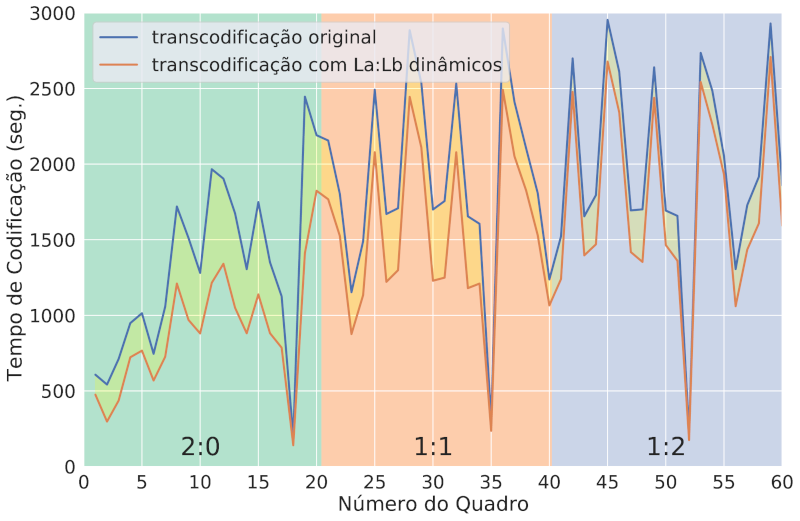
\includegraphics[width=0.75\textwidth]{FIGURES/fig_22.png}
    \caption{Relação do tempo de transcodificação quadro a quadro, comparando a transcodificação original com a transcodificação com troca dinâmica de $La:Lb$. Fonte: Elaborada pelo autor.}
    \label{fig:22}
\end{figure}

\section{Transcodificador VP9 para AV1}
\label{cap:6.2}

No segundo trabalho desenvolvido no contexto desta tese, propusemos um transcodificador rápido de VP9 para AV1, ainda inédito na literatura. Neste trabalho, limitamos os tipos de particionamentos permitidos para serem testados no AV1 de acordo com o observado durante a decodificação do VP9, dependendo da profundidade atual da árvore no codificador AV1. A Figura \ref{fig:14}, apresentada no capítulo \ref{cap:4}, descreve os tipos de particionamentos que o formato AV1 permite, sendo eles: um quadrático (\textit{NONE}), dois binários retangulares (\textit{RECT}), quatro ternários mistos (\textit{AB}) e dois quaternários retangulares (\textit{1TO4}). Note que os tipos não-quadráticos possuem orientação horizontal e vertical. 

Como dito anteriormente, o AV1 é a evolução do formato de codificação de vídeo VP9. Portanto, herda deste diversas ferramentas de codificação. Enquanto o AV1 possui nove tipos de particionamento (capítulo \ref{cap:4}), o VP9 possui apenas três: quadrático, retangular orientado na vertical e retangular orientado na horizontal. Inclusive, há menos tamanhos quadráticos no VP9 (64$\times$64, 32$\times$32, 16$\times$16 e 8$\times$8), não sendo permitidos modos retangulares no menor tamanho. 

Com essas considerações, nesta proposta de transcodificador rápido de VP9 para AV1, avaliamos a correlação entre as orientações dos particionamentos aplicados no VP9 e as orientações dos particionamentos do AV1, para cada nível de profundidade e sob diferentes níveis de quantização.

\subsection{Metodologia}
\label{cap:6.2.1}

O primeiro passo deste trabalho foi correlacionar as orientações de particionamentos realizados pelos codificadores VP9 e AV1, considerando os quatro níveis de quantização utilizados pelas recomendações do AV1 \citet{bib:ietfnetvct}. Considerando quatro vídeos HD1080, foi possível obter as Tabelas \ref{tab:XI}, \ref{tab:XII}, \ref{tab:XIII} e \ref{tab:XIV}, que mostram essa correlação para os CQs 20, 32, 43 e 55, respectivamente, onde cada coluna totaliza 100\%. Como o AV1 possui mais tipos de particionamentos que o VP9, consideramos apenas as orientações horizontais ou verticais dos tipos \textit{AB} e \textit{1TO4}. As células em destaque nessas tabelas indicam quando os codificadores AV1 e VP9 escolhem a mesma profundidade e a mesma orientação de particionamento.

\afterpage{
\clearpage

\begin{landscape}
{\footnotesize

\begin{longtblr}[
    caption = {Correlação (em porcentagem) de orientação de particionamentos entre AV1 (linhas) e VP9 (colunas) por nível de profundidade (valores para o CQ 20).},
    label = {tab:XI}
]{
    colspec = {c|c|r|r|r|r|r|r|r|r|r|r},
    rowhead = 2,
    hlines,
    row{even} = {gray9},
    cell{7}{3}={cyan},
    cell{8}{4}={cyan},
    cell{9}{5}={cyan},
    cell{10}{6}={cyan},
    cell{11}{7}={cyan},
    cell{12}{8}={cyan},
    cell{13}{9}={cyan},
    cell{14}{10}={cyan},
    cell{15}{11}={cyan},
    cell{16}{12}={cyan}
}
\hline
\SetCell[c=2,r=2]{}& & \SetCell[c=10]{c} \textbf{VP9} &&&&&&&&\\
& & \SetCell[c=3]{c}\textbf{1 (64$\times$64)} &&& \SetCell[c=3]{c}\textbf{2 (32$\times$32)} &&& \SetCell[c=3]{c}\textbf{3 (16$\times$16)} &&& \textbf{4 (8$\times$8)} \\
\SetCell[c=2]{c} \textbf{AV1} && \textbf{Quad.} & \textbf{Horz.} & \textbf{Vert.} & \textbf{Quad.} & \textbf{Horz.} & \textbf{Vert.} & \textbf{Quad.} & \textbf{Horz.} & \textbf{Vert.} & \textbf{Quad.} \\
\SetCell[r=3]{c}\textbf{0 (128$\times$128)} & \textbf{Quad.} & 39,18 & 25,16 & 10,92 & 4,56 & 1,86 & 1,72 & 1,61 & 0,79 & 1,40 & 1,49 \\
 & \textbf{Horz.} & 1,15 & 0,38 & 0,39 & 0,16 & 0,06 & 0,06 & 0,04 & 0,12 & 0,01 & 0,03 \\
 & \textbf{Vert.} & 0,07 & 11,62 & 0,00 & 0,03 & 0,02 & 0,01 & 0,09 & 0,01 & 0,03 & 0,01 \\
\SetCell[r=3]{c}\textbf{1 (64$\times$64)} & \textbf{Quad.} & 36,93 & 15,36 & 30,23 & 12,54 & 5,02 & 4,92 & 3,48 & 2,36 & 2,97 & 5,58 \\
 & \textbf{Horz.} & 4,35 & 16,43 & 7,34 & 5,30 & 3,70 & 2,16 & 1,73 & 1,42 & 0,93 & 2,20 \\
 & \textbf{Vert.} & 6,21 & 5,25 & 17,55 & 5,82 & 1,78 & 3,57 & 1,41 & 0,90 & 1,17 & 2,01 \\
\SetCell[r=3]{c}\textbf{2 (32$\times$32)} & \textbf{Quad.} & 7,38 & 13,01 & 18,84 & 31,41 & 19,85 & 21,65 & 15,82 & 12,01 & 10,40 & 11,53 \\
 & \textbf{Horz.} & 1,62 & 6,01 & 4,32 & 13,32 & 25,30 & 13,42 & 16,45 & 15,73 & 9,73 & 10,97 \\
 & \textbf{Vert.} & 1,65 & 2,75 & 5,48 & 10,62 & 10,66 & 20,63 & 14,32 & 7,96 & 15,67 & 9,97 \\
\SetCell[r=3]{c}\textbf{3 (16$\times$16)} & \textbf{Quad.} & 0,83 & 2,17 & 2,65 & 8,52 & 15,77 & 16,33 & 22,78 & 17,48 & 21,09 & 17,19 \\
 & \textbf{Horz.} & 0,31 & 0,85 & 0,93 & 4,03 & 9,53 & 6,60 & 10,68 & 21,50 & 11,43 & 16,19 \\
 & \textbf{Vert.} & 0,24 & 0,71 & 0,99 & 2,79 & 4,64 & 7,16 & 8,82 & 8,64 & 18,87 & 13,23 \\
\SetCell[r=3]{c}\textbf{4 (8$\times$8)} & \textbf{Quad.} & 0,05 & 0,21 & 0,26 & 0,66 & 1,40 & 1,33 & 2,02 & 9,33 & 4,53 & 6,24 \\
 & \textbf{Horz.} & 0,01 & 0,05 & 0,05 & 0,13 & 0,25 & 0,21 & 0,38 & 1,08 & 0,67 & 1,65 \\
 & \textbf{Vert.} & 0,01 & 0,05 & 0,06 & 0,09 & 0,14 & 0,21 & 0,28 & 0,46 & 0,86 & 1,18 \\
\SetCell[r=1]{c}\textbf{5 (4$\times$4)} & \textbf{Quad.} & 0,00 & 0,00 & 0,01 & 0,02 & 0,04 & 0,04 & 0,07 & 0,19 & 0,22 & 0,52 \\
\hline
\end{longtblr}
}
\end{landscape}
}

\afterpage{
\clearpage

\begin{landscape}
{\footnotesize

\begin{longtblr}[
    caption = {Correlação (em porcentagem) de orientação de particionamentos entre AV1 (linhas) e VP9 (colunas) por nível de profundidade (valores para o CQ 32).},
    label = {tab:XII}
]{
    colspec = {c|c|r|r|r|r|r|r|r|r|r|r},
    rowhead = 2,
    hlines,
    row{even} = {gray9},
    cell{7}{3}={cyan},
    cell{8}{4}={cyan},
    cell{9}{5}={cyan},
    cell{10}{6}={cyan},
    cell{11}{7}={cyan},
    cell{12}{8}={cyan},
    cell{13}{9}={cyan},
    cell{14}{10}={cyan},
    cell{15}{11}={cyan},
    cell{16}{12}={cyan}
}
\hline
\SetCell[c=2,r=2]{}& & \SetCell[c=10]{c} \textbf{VP9} &&&&&&&&\\
& & \SetCell[c=3]{c}\textbf{1 (64$\times$64)} &&& \SetCell[c=3]{c}\textbf{2 (32$\times$32)} &&& \SetCell[c=3]{c}\textbf{3 (16$\times$16)} &&& \textbf{4 (8$\times$8)} \\
\SetCell[c=2]{c} \textbf{AV1} && \textbf{Quad.} & \textbf{Horz.} & \textbf{Vert.} & \textbf{Quad.} & \textbf{Horz.} & \textbf{Vert.} & \textbf{Quad.} & \textbf{Horz.} & \textbf{Vert.} & \textbf{Quad.} \\
\SetCell[r=3]{c}\textbf{0 (128$\times$128)} & \textbf{Quad.} & 51,60 & 26,07 & 8,27 & 5,26 & 2,85 & 2,77 & 2,74 & 1,04 & 1,64 & 2,64 \\
 & \textbf{Horz.} & 1,48 & 0,46 & 0,38 & 0,24 & 0,10 & 0,10 & 0,07 & 0,15 & 0,01 & 0,06 \\
 & \textbf{Vert.} & 0,23 & 13,47 & 0,00 & 0,06 & 0,03 & 0,03 & 0,22 & 0,02 & 0,03 & 0,27 \\
\SetCell[r=3]{c}\textbf{1 (64$\times$64)} & \textbf{Quad.} & 27,28 & 14,02 & 26,20 & 11,92 & 5,83 & 5,03 & 5,44 & 4,11 & 5,02 & 9,91 \\
 & \textbf{Horz.} & 3,32 & 11,73 & 6,06 & 6,30 & 5,30 & 2,50 & 2,79 & 2,02 & 1,62 & 3,05 \\
 & \textbf{Vert.} & 4,41 & 4,42 & 16,74 & 6,92 & 2,83 & 4,93 & 2,98 & 1,55 & 2,19 & 3,19 \\
\SetCell[r=3]{c}\textbf{2 (32$\times$32)} & \textbf{Quad.} & 6,56 & 14,77 & 21,18 & 34,00 & 22,50 & 26,26 & 20,19 & 17,56 & 15,13 & 15,27 \\
 & \textbf{Horz.} & 1,83 & 6,18 & 5,92 & 11,60 & 25,49 & 11,20 & 15,15 & 15,83 & 9,36 & 10,30 \\
 & \textbf{Vert.} & 1,51 & 3,48 & 7,55 & 10,22 & 9,16 & 19,76 & 13,61 & 8,31 & 16,27 & 9,99 \\
\SetCell[r=3]{c}\textbf{3 (16$\times$16)} & \textbf{Quad.} & 0,92 & 3,07 & 4,35 & 7,66 & 13,56 & 14,37 & 20,40 & 15,34 & 18,63 & 14,00 \\
 & \textbf{Horz.} & 0,44 & 1,27 & 1,52 & 2,98 & 7,48 & 4,99 & 7,59 & 18,29 & 9,58 & 13,49 \\
 & \textbf{Vert.} & 0,31 & 0,79 & 1,47 & 2,24 & 3,40 & 6,56 & 6,62 & 6,69 & 15,16 & 10,21 \\
\SetCell[r=3]{c}\textbf{4 (8$\times$8)} & \textbf{Quad.} & 0,07 & 0,20 & 0,26 & 0,47 & 1,11 & 1,14 & 1,61 & 7,42 & 3,84 & 4,90 \\
 & \textbf{Horz.} & 0,02 & 0,04 & 0,06 & 0,07 & 0,21 & 0,13 & 0,30 & 1,01 & 0,64 & 1,34 \\
 & \textbf{Vert.} & 0,01 & 0,02 & 0,04 & 0,06 & 0,09 & 0,18 & 0,23 & 0,45 & 0,69 & 0,97 \\
\SetCell[r=1]{c}\textbf{5 (4$\times$4)} & \textbf{Quad.} & 0,00 & 0,00 & 0,01 & 0,01 & 0,03 & 0,03 & 0,07 & 0,21 & 0,18 & 0,42 \\
\hline
\end{longtblr}
}
\end{landscape}
}

\afterpage{
\clearpage

\begin{landscape}
{\footnotesize

\begin{longtblr}[
    caption = {Correlação (em porcentagem) de orientação de particionamentos entre AV1 (linhas) e VP9 (colunas) por nível de profundidade (valores para o CQ 43).},
    label = {tab:XIII}
]{
    colspec = {c|c|r|r|r|r|r|r|r|r|r|r},
    rowhead = 2,
    hlines,
    row{even} = {gray9},
    cell{7}{3}={cyan},
    cell{8}{4}={cyan},
    cell{9}{5}={cyan},
    cell{10}{6}={cyan},
    cell{11}{7}={cyan},
    cell{12}{8}={cyan},
    cell{13}{9}={cyan},
    cell{14}{10}={cyan},
    cell{15}{11}={cyan},
    cell{16}{12}={cyan}
}
\hline
\SetCell[c=2,r=2]{}& & \SetCell[c=10]{c} \textbf{VP9} &&&&&&&&\\
& & \SetCell[c=3]{c}\textbf{1 (64$\times$64)} &&& \SetCell[c=3]{c}\textbf{2 (32$\times$32)} &&& \SetCell[c=3]{c}\textbf{3 (16$\times$16)} &&& \textbf{4 (8$\times$8)} \\
\SetCell[c=2]{c} \textbf{AV1} && \textbf{Quad.} & \textbf{Horz.} & \textbf{Vert.} & \textbf{Quad.} & \textbf{Horz.} & \textbf{Vert.} & \textbf{Quad.} & \textbf{Horz.} & \textbf{Vert.} & \textbf{Quad.} \\
\SetCell[r=3]{c}\textbf{0 (128$\times$128)} & \textbf{Quad.} & 52,23 & 24,66 & 8,86 & 6,60 & 2,99 & 1,92 & 4,72 & 3,45 & 3,99 & 6,82 \\
 & \textbf{Horz.} & 1,55 & 0,41 & 0,42 & 0,37 & 0,03 & 0,05 & 0,04 & 0,12 & 0,00 & 0,02 \\
 & \textbf{Vert.} & 0,39 & 14,63 & 0,03 & 0,08 & 0,03 & 0,06 & 0,26 & 0,08 & 0,08 & 0,22 \\
\SetCell[r=3]{c}\textbf{1 (64$\times$64)} & \textbf{Quad.} & 26,70 & 15,33 & 27,79 & 16,26 & 10,52 & 9,77 & 12,15 & 9,67 & 10,78 & 16,36 \\
 & \textbf{Horz.} & 3,34 & 13,51 & 6,95 & 8,90 & 10,50 & 5,05 & 5,35 & 5,40 & 3,08 & 4,45 \\
 & \textbf{Vert.} & 4,41 & 4,99 & 17,74 & 8,75 & 4,65 & 10,04 & 5,25 & 2,93 & 5,14 & 3,78 \\
\SetCell[r=3]{c}\textbf{2 (32$\times$32)} & \textbf{Quad.} & 6,41 & 14,31 & 20,89 & 34,15 & 23,95 & 28,20 & 21,81 & 23,18 & 18,55 & 17,07 \\
 & \textbf{Horz.} & 1,72 & 5,56 & 4,92 & 7,69 & 21,75 & 8,32 & 11,70 & 13,73 & 7,25 & 8,20 \\
 & \textbf{Vert.} & 1,35 & 2,33 & 6,60 & 7,50 & 6,15 & 16,08 & 10,78 & 5,90 & 13,49 & 8,24 \\
\SetCell[r=3]{c}\textbf{3 (16$\times$16)} & \textbf{Quad.} & 1,04 & 2,45 & 3,37 & 5,66 & 10,72 & 11,57 & 16,74 & 12,09 & 15,59 & 10,88 \\
 & \textbf{Horz.} & 0,44 & 1,08 & 1,03 & 2,02 & 5,25 & 3,41 & 5,22 & 13,67 & 6,99 & 10,82 \\
 & \textbf{Vert.} & 0,34 & 0,54 & 1,16 & 1,59 & 2,35 & 4,44 & 4,48 & 4,45 & 11,14 & 7,92 \\
\SetCell[r=3]{c}\textbf{4 (8$\times$8)} & \textbf{Quad.} & 0,06 & 0,17 & 0,17 & 0,34 & 0,81 & 0,86 & 1,11 & 4,30 & 2,89 & 3,25 \\
 & \textbf{Horz.} & 0,01 & 0,03 & 0,03 & 0,05 & 0,22 & 0,10 & 0,20 & 0,62 & 0,40 & 1,03 \\
 & \textbf{Vert.} & 0,01 & 0,01 & 0,03 & 0,04 & 0,07 & 0,12 & 0,14 & 0,28 & 0,47 & 0,68 \\
\SetCell[r=1]{c}\textbf{5 (4$\times$4)} & \textbf{Quad.} & 0,00 & 0,00 & 0,00 & 0,01 & 0,02 & 0,02 & 0,04 & 0,13 & 0,15 & 0,26 \\
\hline
\end{longtblr}
}
\end{landscape}
}

\afterpage{
\clearpage

\begin{landscape}
{\footnotesize

\begin{longtblr}[
    caption = {Correlação (em porcentagem) de orientação de particionamentos entre AV1 (linhas) e VP9 (colunas) por nível de profundidade (valores para o CQ 55).},
    label = {tab:XIV}
]{
    colspec = {c|c|r|r|r|r|r|r|r|r|r|r},
    rowhead = 2,
    hlines,
    row{even} = {gray9},
    cell{7}{3}={cyan},
    cell{8}{4}={cyan},
    cell{9}{5}={cyan},
    cell{10}{6}={cyan},
    cell{11}{7}={cyan},
    cell{12}{8}={cyan},
    cell{13}{9}={cyan},
    cell{14}{10}={cyan},
    cell{15}{11}={cyan},
    cell{16}{12}={cyan}
}
\hline
\SetCell[c=2,r=2]{}& & \SetCell[c=10]{c} \textbf{VP9} &&&&&&&&\\
& & \SetCell[c=3]{c}\textbf{1 (64$\times$64)} &&& \SetCell[c=3]{c}\textbf{2 (32$\times$32)} &&& \SetCell[c=3]{c}\textbf{3 (16$\times$16)} &&& \textbf{4 (8$\times$8)} \\
\SetCell[c=2]{c} \textbf{AV1} && \textbf{Quad.} & \textbf{Horz.} & \textbf{Vert.} & \textbf{Quad.} & \textbf{Horz.} & \textbf{Vert.} & \textbf{Quad.} & \textbf{Horz.} & \textbf{Vert.} & \textbf{Quad.} \\
\SetCell[r=3]{c}\textbf{0 (128$\times$128)} & \textbf{Quad.} & 55,85 & 25,00 & 12,99 & 10,91 & 7,60 & 4,40 & 9,64 & 9,52 & 10,84 & 10,20 \\
 & \textbf{Horz.} & 1,62 & 0,50 & 0,72 & 0,39 & 0,10 & 0,07 & 0,16 & 0,44 & 0,10 & 0,26 \\
 & \textbf{Vert.} & 0,44 & 17,05 & 0,03 & 0,25 & 0,08 & 0,64 & 0,43 & 0,07 & 0,31 & 0,21 \\
\SetCell[r=3]{c}\textbf{1 (64$\times$64)} & \textbf{Quad.} & 27,07 & 18,28 & 33,51 & 26,73 & 22,43 & 21,70 & 21,62 & 18,89 & 19,88 & 20,50 \\
 & \textbf{Horz.} & 2,79 & 15,70 & 5,92 & 9,41 & 14,52 & 5,94 & 7,50 & 9,47 & 4,92 & 6,56 \\
 & \textbf{Vert.} & 3,29 & 2,91 & 16,52 & 8,16 & 4,01 & 11,55 & 6,00 & 4,08 & 8,61 & 5,21 \\
\SetCell[r=3]{c}\textbf{2 (32$\times$32)} & \textbf{Quad.} & 5,08 & 11,68 & 17,91 & 27,77 & 20,04 & 25,30 & 19,20 & 19,76 & 17,36 & 16,24 \\
 & \textbf{Horz.} & 1,33 & 4,33 & 3,19 & 5,34 & 15,61 & 5,88 & 9,36 & 11,12 & 6,29 & 7,18 \\
 & \textbf{Vert.} & 1,01 & 1,68 & 5,38 & 5,13 & 3,91 & 12,65 & 8,52 & 5,23 & 10,24 & 7,17 \\
\SetCell[r=3]{c}\textbf{3 (16$\times$16)} & \textbf{Quad.} & 0,87 & 1,72 & 2,40 & 3,64 & 6,68 & 7,27 & 11,30 & 8,83 & 9,49 & 8,51 \\
 & \textbf{Horz.} & 0,32 & 0,70 & 0,46 & 1,08 & 3,37 & 1,66 & 3,06 & 7,72 & 3,95 & 8,02 \\
 & \textbf{Vert.} & 0,25 & 0,35 & 0,87 & 0,94 & 1,07 & 2,47 & 2,54 & 2,98 & 6,22 & 6,00 \\
\SetCell[r=3]{c}\textbf{4 (8$\times$8)} & \textbf{Quad.} & 0,05 & 0,08 & 0,07 & 0,18 & 0,41 & 0,37 & 0,48 & 1,45 & 1,30 & 2,37 \\
 & \textbf{Horz.} & 0,01 & 0,01 & 0,01 & 0,03 & 0,10 & 0,05 & 0,10 & 0,28 & 0,19 & 0,83 \\
 & \textbf{Vert.} & 0,01 & 0,01 & 0,02 & 0,03 & 0,04 & 0,05 & 0,08 & 0,15 & 0,26 & 0,58 \\
\SetCell[r=1]{c}\textbf{5 (4$\times$4)} & \textbf{Quad.} & 0,00 & 0,00 & 0,00 & 0,01 & 0,01 & 0,00 & 0,01 & 0,02 & 0,03 & 0,17 \\
\hline
\end{longtblr}

}
\end{landscape}
}


Considerando essas tabelas, torna-se possível identificar qual é a maior probabilidade de ocorrer alguma orientação de particionamento no transcodificador para AV1, dadas as observações no decodificador VP9. Essas orientações mais comuns são mostradas para cada uma das profundidades disponíveis no AV1 e para todos os níveis de quantização utilizados. É possível compreender melhor essas tabelas através do seguinte exemplo: em uma determinada região do vídeo, identifiquemos que o codificador VP9 optou por utilizar o segundo nível de profundidade, havendo dois blocos 32$\times$16, ou seja, com orientação vertical. Ao observarmos a codificação do AV1 no CQ 43 (Tabela \ref{tab:XIII}), há uma probabilidade inferior a 2\% de que o codificador AV1 opte por utilizar uma profundidade 0 com orientação quadrática (bloco 128$\times$128) nessa mesma região do vídeo. Contudo, no terceiro nível de profundidade, o codificador AV1 vai optar por utilizar a orientação quadrática em 28\% das vezes e, em seguida, a orientação vertical em 16\% das vezes. Observações semelhantes podem ser feitas para as quatro tabelas de correlação apresentadas.

Com essas correlações estabelecidas, determinamos que o codificador AV1 somente pode testar blocos orientados de acordo com as maiores probabilidades de orientação observadas nas Tabelas \ref{tab:XI}, \ref{tab:XII}, \ref{tab:XIII} e \ref{tab:XIV}. É possível resumir essas tabelas através da Tabela \ref{tab:XV}, onde destacam-se as únicas orientações autorizadas a serem testadas no codificador AV1, dadas a profundidade atual na codificação e a orientação observada no formato VP9. Note que a profundidade 5 do AV1 possui apenas orientação quadrática, razão pela qual ela não está presente na Tabela \ref{tab:XV}. Como podemos observar, quase todas as probabilidades de escolha do codificador AV1 tendem para a orientação quadrática. Dessa forma, é possível definir um pseudocódigo que simplifica a Tabela \ref{tab:XV}, como apresentado na Figura \ref{fig:23}. Através desse pseudocódigo, podemos apresentar a proposta de transcodificador rápido do formato VP9 para AV1, como consta na Figura \ref{fig:24}.

\afterpage{
\clearpage

\begin{landscape}
{\footnotesize
\begin{longtblr}[
    caption = {Resumo de particionamentos permitidos ao codificador AV1, de acordo com as Tabelas \ref{tab:XI}, \ref{tab:XII}, \ref{tab:XIII} e \ref{tab:XIV}. Destacou-se as células que não são Quad.},
    label = {tab:XV}
]{
    colspec = {l|l|c|l|l|l|l|l|l|l|l|l|l},
    rowhead = 3,
    hlines,
    row{even} = {gray9},
    cell{2}{1}={white},
    cell{4}{1}={white},
    cell{5}{5}={cyan},
    cell{6}{8}={cyan},
    cell{6}{10}={cyan},
    cell{6}{11}={cyan},
    cell{6}{12}={cyan},
    cell{7}{11}={cyan},
    cell{11}{8}={cyan},
    cell{11}{10}={cyan},
    cell{11}{11}={cyan},
    cell{11}{12}={cyan},
    cell{12}{11}={cyan},
    cell{15}{6}={cyan},
    cell{17}{11}={cyan},
}
\hline
\SetCell[c=3]{c} &&& \SetCell[c=10]{c} \textbf{Profundidade e Orientação Observadas no VP9}\\
\SetCell[c=2,r=2]{c} && \SetCell[r=2]{c}\textbf{Profundidade} & \SetCell[c=3]{c}\textbf{1} &&& \SetCell[c=3]{c}\textbf{2} &&& \SetCell[c=3]{c}\textbf{3} &&& \textbf{4} \\
&&& \textbf{Quad.} & \textbf{Horz.} & \textbf{Vert.} & \textbf{Quad.} & \textbf{Horz.} & \textbf{Vert.} & \textbf{Quad.} & \textbf{Horz.} & \textbf{Vert.} & \textbf{Quad.} \\
\SetCell[r=17]{c}\rotatebox{90}{\textbf{Condição do Bloco no AV1}} & \SetCell[r=5]{c}\textbf{CQ 20} & \textbf{0} & Quad. & Quad. & Quad. & Quad. & Quad. & Quad. & Quad. & Quad. & Quad. & Quad. \\
 & & \textbf{1} & Quad. & Horz. & Quad. & Quad. & Quad. & Quad. & Quad. & Quad. & Quad. & Quad. \\
 & & \textbf{2} & Quad. & Quad. & Quad. & Quad. & Horz. & Quad. & Horz. & Horz. & Vert. & Quad. \\
 & & \textbf{3} & Quad. & Quad. & Quad. & Quad. & Quad. & Quad. & Quad. & Horz. & Quad. & Quad. \\
 & & \textbf{4} & Quad. & Quad. & Quad. & Quad. & Quad. & Quad. & Quad. & Quad. & Quad. & Quad. \\
 & \SetCell[r=5]{c}\textbf{CQ 32} & \textbf{0} & Quad. & Quad. & Quad. & Quad. & Quad. & Quad. & Quad. & Quad. & Quad. & Quad. \\
 & & \textbf{1} & Quad. & Quad. & Quad. & Quad. & Quad. & Quad. & Quad. & Quad. & Quad. & Quad. \\
 & & \textbf{2} & Quad. & Quad. & Quad. & Quad. & Horz. & Quad. & Horz. & Horz. & Vert. & Quad. \\
 & & \textbf{3} & Quad. & Quad. & Quad. & Quad. & Quad. & Quad. & Quad. & Horz. & Quad. & Quad. \\
 & & \textbf{4} & Quad. & Quad. & Quad. & Quad. & Quad. & Quad. & Quad. & Quad. & Quad. & Quad. \\
 & \SetCell[r=5]{c}\textbf{CQ 43} & \textbf{0} & Quad. & Quad. & Quad. & Quad. & Quad. & Quad. & Quad. & Quad. & Quad. & Quad. \\
 & & \textbf{1} & Quad. & Quad. & Vert. & Quad. & Quad. & Quad. & Quad. & Quad. & Quad. & Quad. \\
 & & \textbf{2} & Quad. & Quad. & Quad. & Quad. & Quad. & Quad. & Quad. & Quad. & Quad. & Quad. \\
 & & \textbf{3} & Quad. & Quad. & Quad. & Quad. & Quad. & Quad. & Quad. & Horz. & Quad. & Quad. \\
 & & \textbf{4} & Quad. & Quad. & Quad. & Quad. & Quad. & Quad. & Quad. & Quad. & Quad. & Quad. \\
 & \SetCell[r=2]{c}\textbf{CQ 55} & \textbf{0} & Quad. & Quad. & Quad. & Quad. & Quad. & Quad. & Quad. & Quad. & Quad. & Quad. \\
 & & \textbf{1} & Quad. & Quad. & Quad. & Quad. & Quad. & Quad. & Quad. & Quad. & Quad. & Quad. \\
\SetCell[r=3]{c} & \SetCell[r=3]{c}\textbf{CQ 55} & \textbf{2} & Quad. & Quad. & Quad. & Quad. & Quad. & Quad. & Quad. & Quad. & Quad. & Quad. \\
& & \textbf{3} & Quad. & Quad. & Quad. & Quad. & Quad. & Quad. & Quad. & Quad. & Quad. & Quad. \\
 & & \textbf{4} & Quad. & Quad. & Quad. & Quad. & Quad. & Quad. & Quad. & Quad. & Quad. & Quad. \\
\hline
\end{longtblr}
}
\end{landscape}
}



\begin{figure}
    \centering
    \footnotesize
    %\includegraphics[width=0.75\textwidth,trim=4 4 4 4,clip]{ChapterSIX/figs/fig23.png}
    \begin{Verbatim}[frame=single,commandchars=\\\{\}]
        orientacaoAV1 <- \textcolor{red}{Quad.}
	\textcolor{blue}{se} profundidadeAV1 \textcolor{blue}{for} 1 \textcolor{blue}{faça}:
		\textcolor{blue}{se} profundidadeVP9 \textcolor{blue}{for} 1 
			\textcolor{blue}{e} orientacaoVP9 \textcolor{blue}{for} Horz. 
			\textcolor{blue}{e} quantização \textcolor{blue}{for} 20 \textcolor{blue}{faça}:
				orientacaoAV1 <- \textcolor{red}{Horz.}
		\textcolor{blue}{se} profundidadeVP9 \textcolor{blue}{for} 2 
			\textcolor{blue}{e} orientacaoVP9 \textcolor{blue}{for} Vert. 
			\textcolor{blue}{e} quantização \textcolor{blue}{for} 43 \textcolor{blue}{faça}:
				orientacaoAV1 <- \textcolor{red}{Vert.}
	\textcolor{blue}{se} profundidadeAV1 \textcolor{blue}{for} 2 \textcolor{blue}{faça}:
		\textcolor{blue}{se} profundidadeVP9 \textcolor{blue}{for} 2 
			\textcolor{blue}{e} orientacaoVP9 \textcolor{blue}{for} Horz. 
			\textcolor{blue}{e} quantização \textcolor{blue}{for} 20 \textcolor{blue}{faça}:
				orientacaoAV1 <- \textcolor{red}{Horz.}
		\textcolor{blue}{se} profundidadeVP9 \textcolor{blue}{for} 2 
			\textcolor{blue}{e} orientacaoVP9 \textcolor{blue}{for} Horz. 
			\textcolor{blue}{e} quantização \textcolor{blue}{for} 32 \textcolor{blue}{faça}:
				orientacaoAV1 <- \textcolor{red}{Horz.}
		\textcolor{blue}{se} profundidadeVP9 \textcolor{blue}{for} 3 
			\textcolor{blue}{e} orientacaoVP9 \textcolor{blue}{for} Quad. 
			\textcolor{blue}{e} quantização \textcolor{blue}{for} 20 \textcolor{blue}{faça}:
				orientacaoAV1 <- \textcolor{red}{Horz.}
		\textcolor{blue}{se} profundidadeVP9 \textcolor{blue}{for} 3 
			\textcolor{blue}{e} orientacaoVP9 \textcolor{blue}{for} Horz. 
			\textcolor{blue}{e} quantização \textcolor{blue}{for} 20 \textcolor{blue}{faça}:
				orientacaoAV1 <- \textcolor{red}{Horz.}
		\textcolor{blue}{se} profundidadeVP9 \textcolor{blue}{for} 3 
			\textcolor{blue}{e} orientacaoVP9 \textcolor{blue}{for} Vert. 
			\textcolor{blue}{e} quantização \textcolor{blue}{for} 20 \textcolor{blue}{faça}:
				orientacaoAV1 <- \textcolor{red}{Vert.}
		\textcolor{blue}{se} profundidadeVP9 \textcolor{blue}{for} 3 
			\textcolor{blue}{e} orientacaoVP9 \textcolor{blue}{for} Vert. 
			\textcolor{blue}{e} quantização \textcolor{blue}{for} 32 \textcolor{blue}{faça}:
				orientacaoAV1 <- \textcolor{red}{Vert.}
	\textcolor{blue}{se} profundidadeAV1 \textcolor{blue}{for} 3 \textcolor{blue}{faça}:
		\textcolor{blue}{se} profundidadeVP9 \textcolor{blue}{for} 3 
			\textcolor{blue}{e} orientacaoVP9 \textcolor{blue}{for} Horz. 
			\textcolor{blue}{e} quantização \textcolor{blue}{for} 20 \textcolor{blue}{faça}:
				orientacaoAV1 <- \textcolor{red}{Horz.}
		\textcolor{blue}{se} profundidadeVP9 \textcolor{blue}{for} 3 
			\textcolor{blue}{e} orientacaoVP9 \textcolor{blue}{for} Horz. 
			\textcolor{blue}{e} quantização \textcolor{blue}{for} 32 \textcolor{blue}{faça}:
				orientacaoAV1 <- \textcolor{red}{Horz.}
		\textcolor{blue}{se} profundidadeVP9 \textcolor{blue}{for} 3 
			\textcolor{blue}{e} orientacaoVP9 \textcolor{blue}{for} Horz. 
			\textcolor{blue}{e} quantização \textcolor{blue}{for} 43 \textcolor{blue}{faça}:
				orientacaoAV1 <- \textcolor{red}{Horz.}
	\textcolor{blue}{retorna} orientacaoAV1
    \end{Verbatim}
    \caption{Pseudocódigo implementado no AV1 para escolha de orientação de particionamentos, baseado na Tabela \ref{tab:XV}. Fonte: Elaborada pelo autor.}
    \label{fig:23}
\end{figure}

\begin{figure}
    \centering
    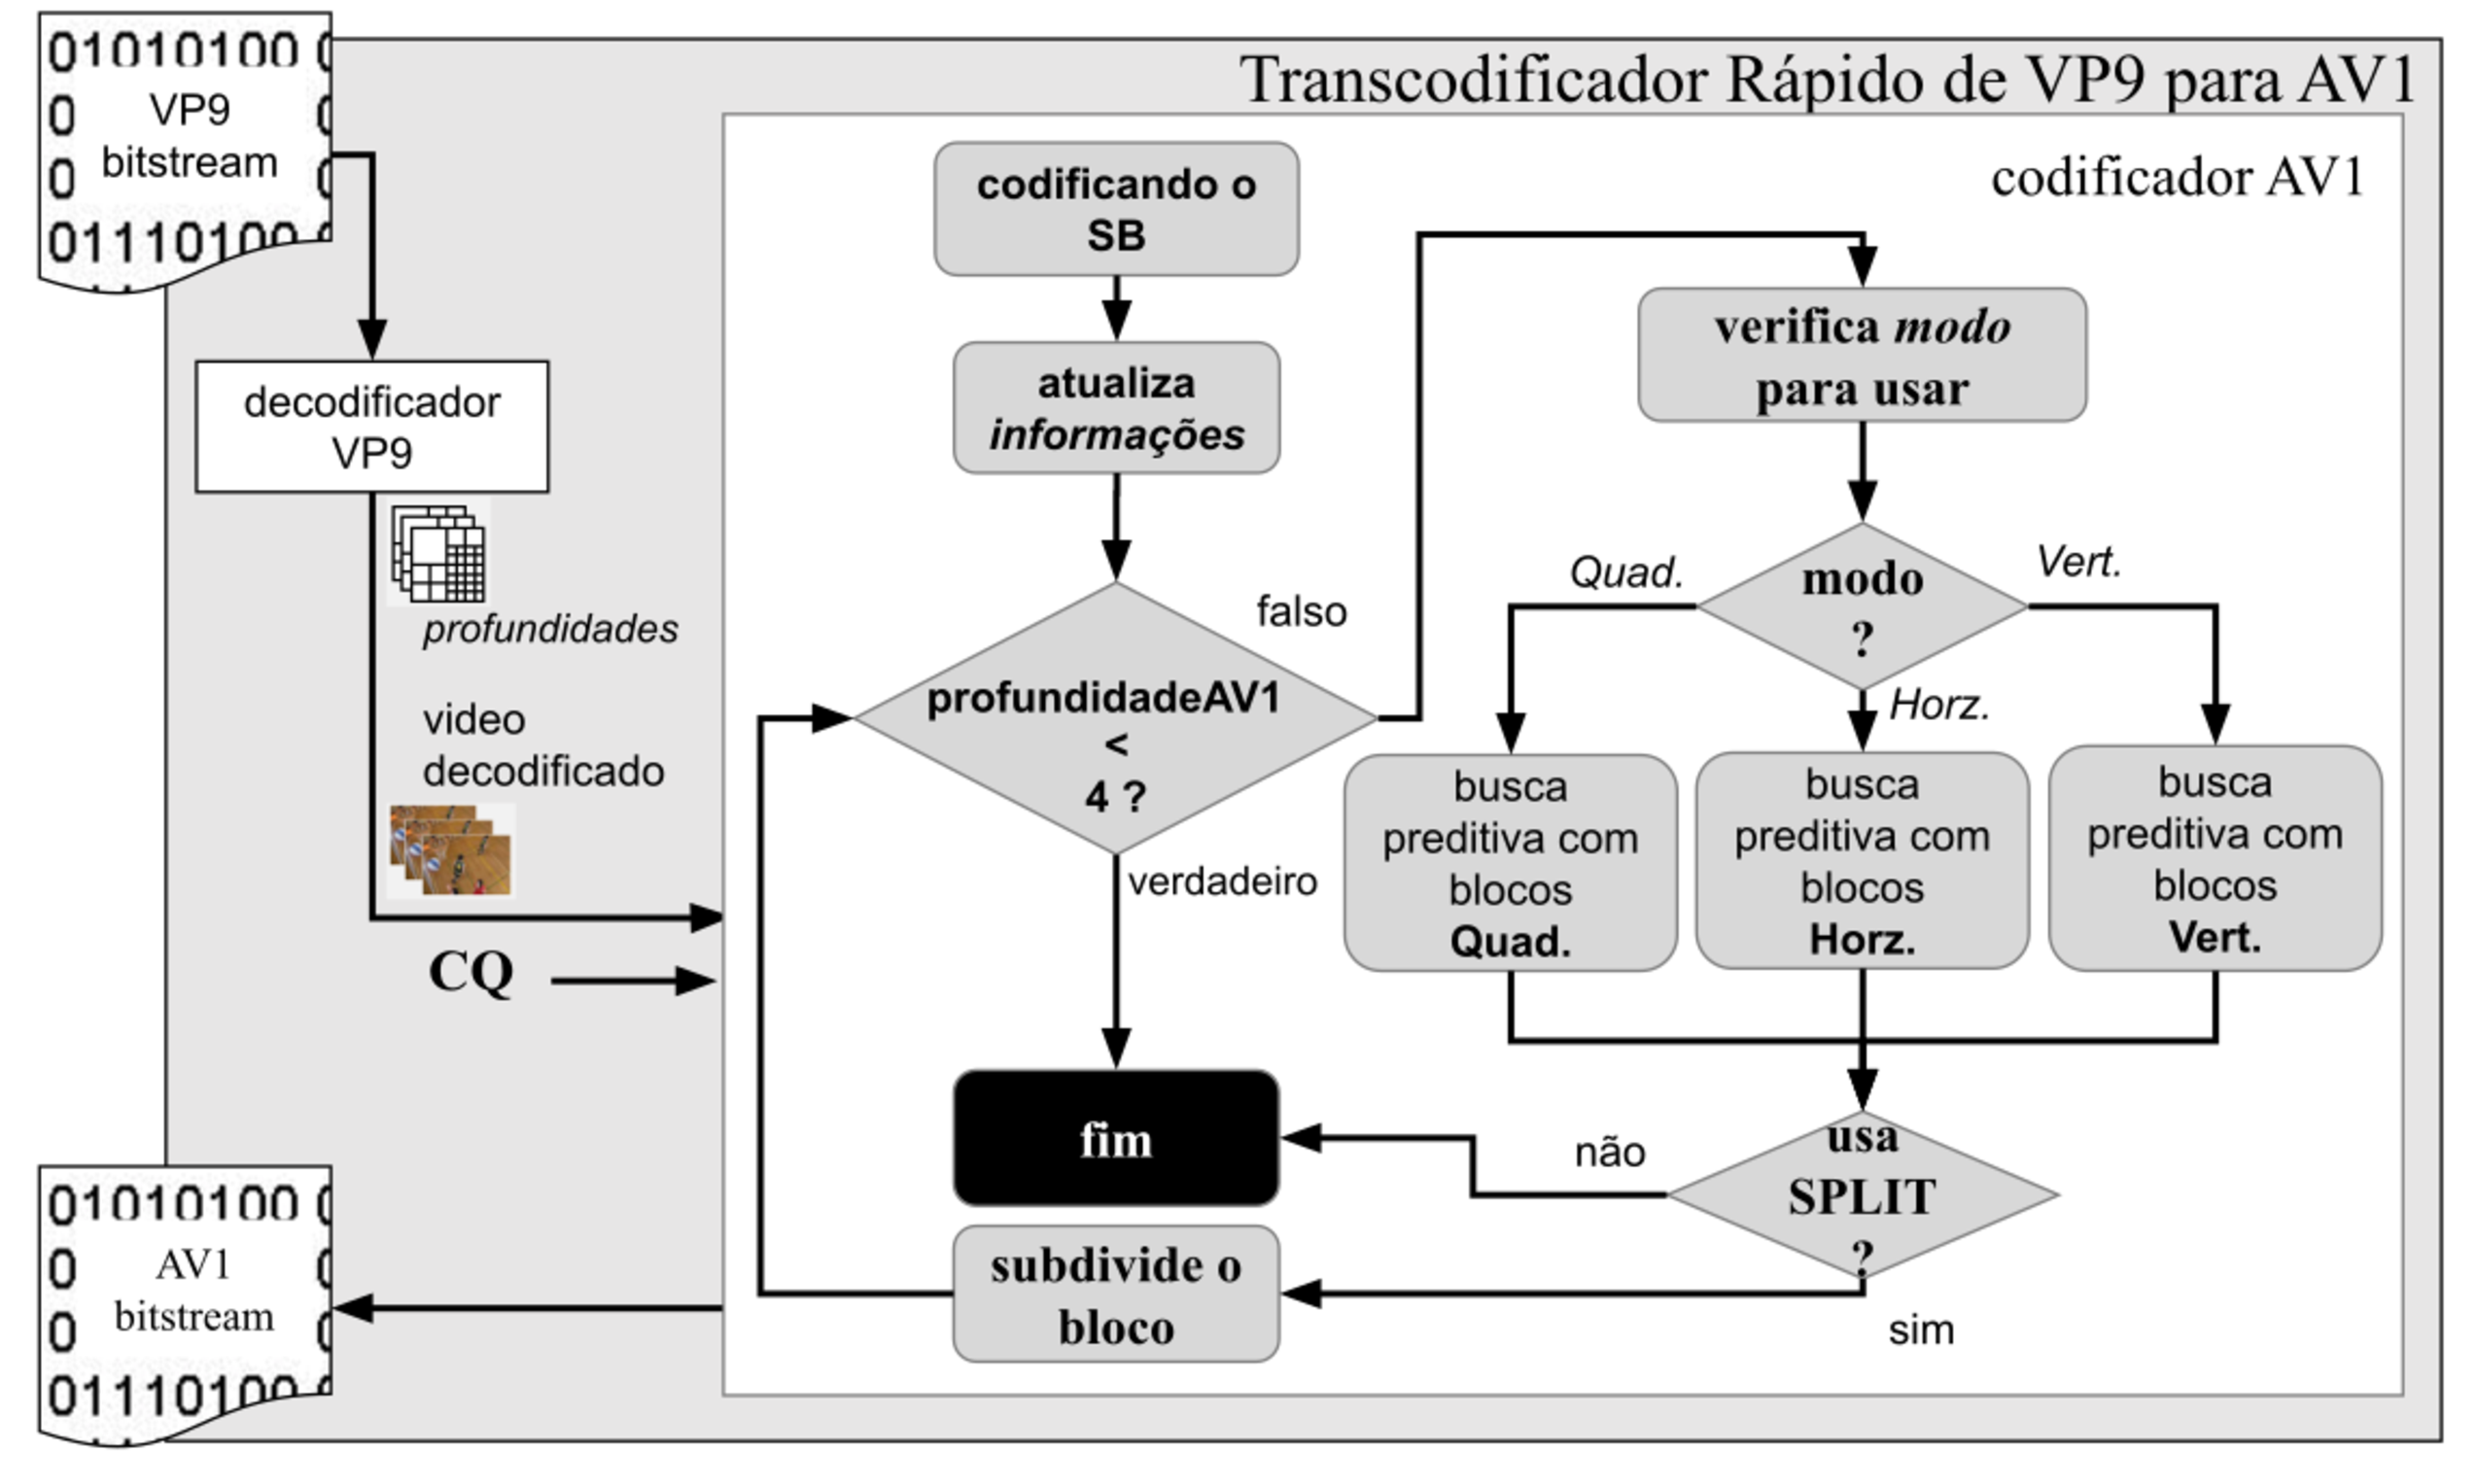
\includegraphics[width=0.85\textwidth]{FIGURES/fig_24.png}
    \caption{Proposta de transcodificação rápida do formato VP9 para AV1 baseada em análises estatísticas. Fonte: Elaborada pelo autor.}
    \label{fig:24}
\end{figure}

O algoritmo representado no fluxograma da Figura \ref{fig:24} tem como entrada informações do decodificador, indicando as profundidades e orientações de cada árvore de particionamentos decodificada. Durante a execução do codificador, informações sobre o nível de quantização utilizado e o nível atual da árvore são utilizados para avaliar a correta orientação a ser utilizada naquele ponto do vídeo. A única exceção é caso a profundidade atual seja igual a cinco, como representado no primeiro condicional da Figura \ref{fig:24}. 

\subsection{Resultados}
\label{cap:6.2.2}

Para possibilitar a realização dos experimentos de avaliação deste transcodificador rápido, foram utilizados 60 quadros de 20 sequências de vídeos em diversas resoluções, separadas em categorias de resolução. Com isso, foi possível obter os resultados apresentados na Tabela \ref{tab:XVI}, onde se observa uma redução média de 28,16\% do tempo total da transcodificação em relação à transcodificação original, a um custo de elevar o BD-rate em 4,34\%.

\afterpage{
\clearpage

\begin{landscape}
{\footnotesize
\begin{longtblr}[
    caption = {Resultados da transcodificação rápida de VP9 para AV1 baseada em análise estatística.},
    label = {tab:XVI}
]{
    colspec = {l|l|r|r|r},
    rowhead = 1,
    hlines,
    row{even} = {gray9}
}
\hline

\textbf{Classe} & \textbf{Sequência} & \textbf{BD-rate (\%)} & \textbf{TS (\%)} & \textbf{Razão} \\
\SetCell[r=4]{l}CIF & bqfree\_240p\_120f & 4,7555 & 24,18 & 0,197 \\
 & bqzoom\_240p\_120f & 4,4228 & 23,37 & 0,189 \\
 & chairlift\_240p\_120f & 4,0765 & 26,89 & 0,152 \\
 & mozzoom\_240p\_120f & 2,7979 & 26,15 & 0,107 \\
\SetCell[c=2]{r}Média – CIF && 4,0132 & 25,15 & \\
\SetCell[c=2]{r}Desvio Padrão – CIF && 0,8563 & 1,64 & \\
\SetCell[r=4]{l}SD & rain2\_hdr\_amazon\_360p & 2,9938 & 32,73 & 0,091 \\
 & red\_kayak\_360p\_120f & 1,9096 & 31,62 & 0,060 \\
 & snow\_mnt\_640x360\_120f & 1,6583 & 33,61 & 0,049 \\
 & tacomanarrows360p\_120f & 3,5571 & 18,65 & 0,191 \\
\SetCell[c=2]{r}Média – SD && 2,5297 & 29,15 & \\
\SetCell[c=2]{r}{Desvio Padrão – SD} && 0,8972 & 7,05 & \\
\SetCell[r=4]{l}{HD720} & dark720p\_120f & 4,1424 & 23,02 & 0,180 \\
 & Johnny\_1280x720\_60\_120f & 6,0483 & 24,74 & 0,245 \\
 & Netflix\_DrivingPOV\_1280x720\_60fps\_8bit\_420\_120f & 6,3701 & 31,58 & 0,202 \\
 & Netflix\_RollerCoaster\_1280x720\_60fps\_8bit\_420\_120f & 6,6917 & 41,73 & 0,160 \\
\SetCell[c=2]{r}Média – HD720 && 5,8131 & 30,27 & \\
\SetCell[c=2]{r}Desvio Padrão – HD720 && 1,1444 & 8,49 & \\
\SetCell[r=2]{l}HD1080 & crowd\_run\_1080p50\_60f & 3,5322 & 34,25 & 0,103 \\
 & Netflix\_Crosswalk\_1920x1080\_60fps\_8bit\_420\_60f & 4,0039 & 18,01 & 0,222 \\
\SetCell[r=2]{l}HD1080& park\_joy\_1080p50\_60f & 5,8649 & 42,67 & 0,137 \\
 & seaplane\_hdr\_amazon\_1080p & 4,9808 & 24,53 & 0,203 \\
\SetCell[c=2]{r}Média – HD1080 && 4,5955 & 29,86 & \\
\SetCell[c=2]{r}Desvio Padrão – HD1080 && 1,0393 & 10,83 & \\
\SetCell[r=4]{l}HD1080+SCC & DOTA2\_60f\_420 & 3,3484 & 25,49 & 0,131 \\
 & MINECRAFT\_60f\_420 & 4,8084 & 47,58 & 0,101 \\
 & STARCRAFT\_60f\_420 & 2,8454 & 21,22 & 0,134 \\
 & wikipedia\_420 & 8,0104 & 11,26 & 0,711 \\
\SetCell[c=2]{r}Média – HD1080+SCC && 4,7532 & 26,39 & \\
\SetCell[c=2]{r}Desvio Padrão – HD1080+SCC && 2,3256 & 15,33 & \\
\SetCell[c=2]{r}\textbf{Média Geral} && \textbf{4,3409} &\textbf{ 28,16} & \\
\SetCell[c=2]{r}\textbf{Desvio Padrão Geral} && \textbf{1,6411} & \textbf{8,92} & \\

\hline
\end{longtblr}
}
\end{landscape}
}


Cabe destacar que esta é a primeira solução desenvolvida para acelerar a transcodificação de VP9 para AV1. Conforme pode ser visto na Tabela \ref{tab:XVI}, a técnica proposta se mostrou mais eficiente para vídeos abaixo da categoria de alta resolução, em especial nos vídeos de 640$\times$360 pixels, apresentando um BD-rate médio de 2,5\%. O vídeo de maior destaque na codificação, com base no valor Razão, foi \textit{snow\_mnt\_640x360\_120f}, cuja transcodificação foi acelerada em 33\% a um custo de elevar o BD-rate em apenas 1,65\%. Por outro lado, o vídeo \textit{wikipedia\_420}, de resolução HD1080+SCC, apresentou o pior desempenho: acelerou apenas 11\% da transcodificação a um custo de 8\% em BD-rate. 

\chapter{Transcodificação de Vídeo Baseado em Aprendizado de Máquina}
\label{cap:7}

Ao longo do texto, apresentamos o uso de aprendizado de máquina como uma importante estratégia para tornar as propostas de aceleração da transcodificação mais eficientes. Como foi ressaltado no capítulo \ref{cap:3}, trabalhos envolvendo aprendizado de máquina tendem a apresentar resultados mais satisfatórios de TS e BD-rate do que aqueles baseados em análises estatísticas. Apesar dos resultados de propostas baseadas em aprendizado de máquina serem positivos, a adaptação das estratégias em outros transcodificadores rápidos é algo incomum, principalmente em transcodificações heterogêneas, já que pode ser difícil, ou mesmo impossível, compatibilizar as complexas ferramentas de diferentes formatos de codificação de vídeo. Portanto, um dos objetivos apresentados neste capítulo é desenvolver um \textit{pipeline} de processamento que possibilite a adaptação da metodologia de desenvolvimento de transcodificadores rápidos para diversas combinações de formatos utilizando aprendizado de máquina. Embora abordemos especificamente o algoritmo de aprendizado de máquina CART (veja seção \ref{cap:7.1}), a alteração de algoritmos e/ou de seus hiperparâmetros, dentro do \textit{pipeline}, é simples e intuitiva.

Para fins de viabilidade e prova de conceito do \textit{pipeline} de processamento proposto, este capítulo apresenta soluções geradas para transcodificadores de diversos formatos para o formato AV1, adaptando um trabalho original desenvolvido de VP9 para AV1. Contudo, ao invés de apresentar múltiplas soluções distintas, ou seja, um transcodificador rápido para cada combinação de formatos (como os apresentados no capítulo \ref{cap:6}), este capítulo propõe a aplicação do \textit{pipeline} proposto, a fim de permitir a geração de soluções para os vários transcodificadores rápidos de forma simplificada.

Como descrito no capítulo \ref{cap:3}, o reaproveitamento de estruturas de particionamento de blocos é uma das principais abordagens em trabalhos de transcodificador rápido observados na literatura científica. Uma das principais razões dessa relevância está no fato de que o número de tamanhos de blocos avaliados está diretamente relacionados com a alta complexidade das predições intraquadro e interquadros, inclusive das transformadas, já que a busca pelos melhores modos preditivos se dá pela busca (por vezes exaustiva) dos diversos tamanhos de blocos disponíveis. Logo, reduzir a quantidade de tamanhos de bloco a serem considerados na recodificação do vídeo reduz consideravelmente a complexidade do codificador. No capítulo \ref{cap:5}, abordamos o impacto na eficiência da codificação do AV1 ao manipular a sua árvore de particionamentos. Portanto, as soluções desenvolvidas para transcodificação rápida usando modelos preditivos gerados por algoritmos de aprendizado de máquina, descritas neste capítulo da tese, possuem como base o treinamento de modelos com o objetivo de predizer o particionamento do bloco em quatro novos ramos.

Assim, apresentamos dois desafios neste capítulo: (1) verificar a possibilidade de implementar um \textit{pipeline} de processamento que permita a adaptação de soluções para transcodificadores rápidos de forma simplificada e escalonável, ou seja, se é possível utilizar os mesmos passos empregados no desenvolvimento de um transcodificador rápido ao desenvolver um outro transcodificador rápido para outra combinação de formatos; e (2) averiguar se o \textit{pipeline} permite atingir resultados compatíveis com o observado na literatura, independentemente da combinação de formatos utilizados como fonte e destino. 

As soluções para aceleração de transcodificadores geradas a partir do \textit{pipeline} proposto baseiam-se nos formatos mais comuns na indústria de \textit{streaming} da atualidade, conforme \citet{bib:bitmovin_report_2021} e \citet{bib:bitmovin_report_2022}: H.264/AVC, H.265/HEVC, VP9, VP8, VVC e AV1. Como deve ter ficado evidente até este momento, optamos por utilizar  o AV1 como formato de destino.

Além do nosso trabalho apresentado na seção \ref{cap:5.2}, não existem outros trabalhos conhecidos com foco na aceleração da transcodificação de VP9 para AV1. Há na literatura alguns trabalhos de transcodificação rápida de H.265/HEVC para AV1, vide \citet{bib:borges_2019}, \citet{bib:borges2_2019}, \citet{bib:borges2_2021} e \citet{bib:chen_2019}. Inclusive, os autores deste último desenvolveram uma solução envolvendo aprendizado de máquina (trabalho já abordado nas seções \ref{cap:3.1} e \ref{cap:6.1}). As demais soluções transcodificação que adaptamos por meio do uso de nosso \textit{pipeline} são de transcodificações rápidas inéditas, até o presente momento, na literatura: VP8-para-AV1, H.264/AVC-para-AV1 e H.266/VVC-para-AV1.

Conforme discutido no capítulo \ref{cap:1} com base no relatório publicado por \citet{bib:bitmovin_report_2021} e \citet{bib:bitmovin_report_2022}, os formatos listados (H.264/AVC, H.265/HEVC, VP9 e VP8) são os mais utilizados na indústria de \textit{streaming} de vídeos. Portanto, apresentamos soluções para aceleração de transcodificação para o formato de codificação de vídeo AV1 a partir de praticamente 100\% dos formatos utilizados no mercado internacional de streaming de vídeo, com exceção da China, que utiliza formatos próprios \cite{bib:china_codecs}.

Assim exposto, este capítulo apresenta as seguintes contribuições nas próximas seções:

\begin{enumerate}[1.]
    \item Um \textit{pipeline} de processamento para geração de soluções de transcodificadores rápidos de vídeo com uso de modelos preditivos treinados através de aprendizado de máquina;

    \item Um transcodificador VP9-para-AV1, acelerado através do uso de árvores de decisão;

    \item Um transcodificador H.264/AVC-para-AV1, acelerado através do uso de árvores de decisão;

    \item Um transcodificador H.265/HEVC-para-AV1, acelerado através do uso de árvores de decisão;

    \item Um transcodificador VP8-para-AV1, acelerado através do uso de árvores de decisão;

    \item Um transcodificador H.266/VVC-para-AV1, acelerado através do uso de árvores de decisão.
    
\end{enumerate}

Para permitir o desenvolvimento e a prova de conceito do \textit{pipeline} de processamento proposto, algumas decisões precisaram ser tomadas, descritas na seção \ref{cap:7.1}. A seção \ref{cap:7.2} se dedica a abordar o funcionamento do \textit{pipeline} proposto e suas fases de execução automatizadas. Os detalhes mais importantes desse \textit{pipeline} de processamento são aprofundados nas seções \ref{cap:7.3} (seleção dos modelos de aprendizado de máquina) e \ref{cap:7.4} (algoritmo de transcodificação a ser adaptado pelas propostas).

\section{Metodologia e Ferramental Utilizado}
\label{cap:7.1}

Apesar de os vídeos de ultra alta definição estarem crescendo em uso, principalmente UHD4K (de 3840$\times$2160 ou 4096$\times$2160 pixels), é a resolução de alta-definição 1080 (HD1080, de 1920$\times$1080 pixels) que é a mais consumida pelos usuários de serviços de \textit{streaming} \cite{bib:bitmovin_twitter}. Portanto, nas soluções desenvolvidas neste capítulo, dedicamos esforços para apresentar resultados nessa categoria de vídeos, mais especificamente em sequências de vídeo naturais HD1080. No entanto, sequências de vídeos naturais HD720 e UHD4K também serão consideradas, sempre que possível, para avaliação dos modelos preditivos. É importante destacar que, como qualquer outro trabalho envolvendo aprendizado de máquina, os conjuntos de dados precisam ser divididos em três subconjuntos, conforme discutido na seção \ref{cap:2.2}: de treinamento, de teste e de predição. Visando construir um vasto conjunto de vídeos, independentes entre si, utilizamos todos os vídeos HD1080 disponíveis nas condições comuns de teste dos documentos \cite{bib:av2_avm}, \citet{bib:hevcctc} e \citet{bib:ietfnetvct}, para compor, respectivamente, os conjuntos de treino (sete sequências), de teste (sete sequências) e de predição (demais sequências). Como pode ser visto na Tabela \ref{tab:XVII}, fazem parte dos vídeos de predição 48 sequências, distribuídas entre as resoluções HD720, HD1080 e UHD4K. Como foi dito no capítulo \ref{cap:4}, o Apêndice \ref{apx:A} descreve com detalhes as sequências utilizadas. Na Tabela \ref{tab:XVII}, constam os nomes das sequências utilizadas em cada uma das fases de desenvolvimento das soluções propostas neste capítulo.

\begin{table}
\begin{center}
\caption{Sequências de vídeo selecionadas para compor os conjuntos dos experimentos.}
\label{tab:XVII}
\footnotesize

\begin{tblr}{
    colspec = {l|p{13cm}},
    hlines,
    row{even} = {gray9}
}
\hline
\textbf{Fase} & \textbf{Sequências}  \\
Treinamento & BasketballDrive\_1920x1080\_50, BQTerrace\_1920x1080\_60, Cactus\_1920x1080\_50, CrowdRun\_1920x1080\_25, Kimono1\_1920x1080\_24, ParkScene\_1920x1080\_24, Tennis\_1920x1080\_24 \\
Teste        & FountainSky\_1920x1080p30\_130f, TimeLapseStreet\_1920x1080p30\_130f, Wheat\_1920x1080, WorldCup\_1920x1080\_30p, WorldCup\_far\_1920x1080\_30p, WorldCupFarSky\_1920x1080\_30p, Skater227\_1920x1080\_30fps \\
Predição    & aspen\_1080p\_60f, crowd\_run\_1080p50\_60f, dark720p\_120f, ducks\_take\_off\_1080p50\_60f, FourPeople\_1280x720\_60, FourPeople\_1280x720\_60\_120f, gipsrestat720p\_120f, Johnny\_1280x720\_60, Johnny\_1280x720\_60\_120f, KristenAndSara\_1280x720\_60, KristenAndSara\_1280x720\_60\_120f, Netflix\_Aerial\_1920x1080\_60fps\_8bit\_420\_60f, Netflix\_Boat\_1920x1080\_60fps\_8bit\_420\_60f, Netflix\_Crosswalk\_1920x1080\_60fps\_ 8bit\_420\_60f, Netflix\_DinnerScene\_1280x720\_60fps\_8bit\_420\_120f, Netflix\_DrivingPOV\_1280x720\_60fps\_8bit\_420\_120f, Netflix\_FoodMarket\_1920x1080\_60fps\_8bit\_420\_60f, Netflix\_FoodMarket2\_1280x720\_60fps\_8bit\_420\_120f, Netflix\_PierSeaside\_1920x1080\_60fps\_8bit\_420\_60f, Netflix\_RollerCoaster\_1280x720\_60fps\_8bit\_420\_120f, Netflix\_SquareAndTimelapse\_1920x1080\_60fps\_8bit\_420\_60f, Netflix\_Tango\_1280x720\_60fps\_8bit\_420\_120f, Netflix\_TunnelFlag\_1920x1080\_60fps\_8bit\_420\_60f, old\_town\_cross\_1080p50\_60f, park\_joy\_1080p50\_60f, pedestrian\_area\_1080p25\_60f, rush\_field\_cuts\_1080p\_60f, rush\_hour\_1080p25\_60f, station2\_1080p25\_60f, Vidyo1\_1280x720\_60, vidyo1\_720p\_60fps\_120f, Vidyo3\_1280x720\_60, vidyo3\_720p\_60fps\_120f, Vidyo4\_1280x720\_60, vidyo4\_720p\_60fps\_120f, boat\_hdr\_amazon\_720p, guitar\_hdr\_amazon\_1080p, pan\_hdr\_amazon\_1080p, rain\_hdr\_amazon\_720p, seaplane\_hdr\_amazon\_1080p, Netflix\_BarScene\_4096x2160\_60fps\_10bit\_420\_60f, Netflix\_BoxingPractice\_4096x2160\_60fps\_10bit\_420\_60f, Netflix\_Dancers\_4096x2160\_60fps\_10bit\_420\_60f, Netflix\_Narrator\_4096x2160\_60fps\_10bit\_420\_60f, Netflix\_RitualDance\_4096x2160\_60fps\_10bit\_420\_60f, Netflix\_ToddlerFountain\_4096x2160\_60fps\_10bit\_420\_60f, Netflix\_WindAndNature\_4096x2160\_60fps\_10bit\_420\_60f, street\_hdr\_amazon\_2160p \\
\hline
\end{tblr}
\end{center}
\end{table}


\subsection{Algoritmos de Aprendizado de Máquina}
\label{cap:7.1.3}

No capítulo \ref{cap:4}, especificamos que a linguagem Python versão 3 foi utilizada para o desenvolvimento de algumas soluções apresentadas nesta tese, em particular as apresentadas no atual capítulo. Dentre essas soluções, está o treinamento de modelos preditivos gerados por algoritmos de aprendizado de máquina. Existem diversas ferramentas, desenvolvidas em Python, que possibilitam essa geração de modelos preditivos, dentre elas o pacote \textit{Scikit-Learn} \cite{bib:scikitlearn-site}. Esse pacote oferece um algoritmo para treinamento de árvores de decisão que permitem a classificação e a regressão de valores, denominado \textit{Classification and Regression Trees} (CART) \cite{bib:scikitlearn_cart}, baseado no trabalho de \citet{bib:livroCART}. Este algoritmo permite a manipulação de alguns hiperparâmetros, descritos na Tabela \ref{tab:XVIII}. Nesta tabela apresentamos os hiperparâmetros existentes no algoritmo CART e seus respectivos valores usados nas soluções propostas de transcodificação rápida com uso de modelos gerados pelo algoritmo CART. Na última coluna da Tabela \ref{tab:XVIII}, apresentamos a quantidade de variações existentes para cada hiperparâmetro, considerando os valores que utilizaremos. Logo, calculando-se o produto dessas variações, há um total de 9,5 milhões de modelos candidatos de aprendizado de máquina a serem treinados com este algoritmo. Observe que, em vários hiperparâmetros da Tabela \ref{tab:XVIII} que utilizam valores inteiros como entrada, consideramos um valor máximo de 25. A razão disso é a quantidade de atributos utilizados nos trabalhos deste capítulo, que é de 25, conforme consta na seção \ref{cap:7.3}.

\afterpage{
\clearpage

\begin{landscape}
{\footnotesize
\begin{longtblr}[
    caption = {Relação dos hiperparâmetros disponíveis no algoritmo CART.},
    label = {tab:XVIII}
]{
    colspec = {l|p{14cm}|p{4.2cm}|r},
    rowhead = 1,
    hlines,
    row{even} = {gray9}
}
\hline
\textbf{Hiperparâmetro} & \textbf{Descrição} & \textbf{Valores Utilizados} & \textbf{Quantidade} \\
\textit{Criterion} & Define a função para medir a qualidade do subparticionamento árvore de decisão. Podem ser utilizados ganho de impureza gini ou ganho de informação por entropia de Shannon, conforme descritos em \citet{bib:CART_matematica}. & 'gini', 'entropy' & 2 \\
\textit{Splitter} & Define a estratégia utilizada para escolher o subparticionamento em cada nó da árvore de decisão. É possível optar pela melhor divisão ou divisão aleatória. & 'best', 'random' & 2 \\
\textit{Max Depth} & Define a profundidade máxima da árvore de decisão. O valor ‘None’ indica que não há um limite definido. & 'None', 3, 5, 7, 11, 13, 17, 19, 25 & 9 \\
\textit{Min Samples Split} & Define o número mínimo de amostras necessárias para subparticionar um nó interno (no mínimo duas amostras). & 2, 3, 5, 7, 11, 13, 17, 19, 25 & 9 \\
\textit{Min Samples Leaf} & Define o número mínimo de amostras necessárias para tornar um nó como folha. Ou seja, o subparticionamento em qualquer profundidade só será considerado se, pelo menos este número de amostras, estiver tanto no ramo do lado esquerdo como no lado direito.  & 1, 3, 5, 7, 11, 13, 17, 19, 25 & 9 \\
\textit{Max Features} & Define o número de atributos a serem considerados ao procurar o melhor subparticionamento do nó. Pode ser a raiz quadrada, ou o logaritmo de base dois da quantidade de atributos disponíveis, ou nenhum, indicando que todos os atributos devem ser utilizados. & 'sqrt', 'log2', 'None' & 3 \\
\textit{Max Leaf Nodes} & Define o número máximo de nós folhas. Em caso de ‘None’, não há limite máximo. A escolha pelos melhores nós é definida pelo próximo atributo. & 'None', 3, 5, 7, 11, 13, 17, 19, 25 & 9 \\
\textit{Min Impurity Decrease} & Define se um nó deve ser subparticionamento ou não, caso esta divisão induza a uma diminuição na impureza maior ou igual ao valor definido. & 0,0, 0,1, 0,2, 0,3, 0,4, 0,5, 0,6, 0,7, 0,8, 0,9, 1,0 & 11 \\
\textit{CPP Alpha} & Define o valor a ser usado para poda antecipada considerando a mínima taxa entre custo e complexidade (\textit{Minimal Cost-Complexity Pruning}, conforme \citet{bib:CART_cppalpha}). A subárvore com uma taxa inferior ao definido será escolhida. Se 0.0, nenhuma poda é executada. & 0,0, 0,1, 0,2, 0,3, 0,4, 0,5, 0,6, 0,7, 0,8, 0,9, 1,0 & 11 \\
\SetCell[c=3]{r}Quantidade Total de Modelos &&& 9.526.572 \\
\hline
\end{longtblr}
}
\end{landscape}
}


\subsection{Mensuração de Resultados}
\label{cap:7.1.4}

Na seção \ref{cap:2.4} discutimos as métricas estatísticas \textit{F1-Score} (Equação \ref{eq:6}) e AUC (Figura \ref{fig:8}) para avaliação dos treinamentos dos modelos preditivos gerados por algoritmos de aprendizado de máquina. O pacote \textit{scikit-learn} oferece meios de mensurar essas métricas, por meio do módulo ``\textit{sklearn.metrics}'', que permite utilizar as funções ``\textit{f1\_score}'' \cite{bib:scikitlearn_f1} e ``\textit{roc\_auc\_score}'' \cite{bib:scikitlearn_auc}. Essas duas funções possuem diversos parâmetros de utilização, conforme pode ser observado em documentação própria \cite{bib:scikitlearn_f1, bib:scikitlearn_auc}. Serão utilizados os valores padrões dessas funções, exceto por um único parâmetro: ``\textit{average}''. Por padrão, esse parâmetro avalia apenas os resultados positivos preditos pelo modelo treinado; no entanto, apesar dos modelos treinados pelas nossas propostas terem rótulos binários (ver mais na seção \ref{cap:7.3}), a relevância das respostas positivas tanto quanto as negativas possuem igual importância. Dessa forma, como é importante que as funções ``\textit{f1\_score}'' e ``\textit{roc\_auc\_score}'' avaliem ambas respostas do rótulo igualmente, o parâmetro ``\textit{average}'' deve ser configurado como ``\texttt{macro}''.

Em relação às métricas para comparação dos resultados de transcodificação rápida, empregamos os valores de TS (Equação \ref{eq:7}) e de BD-rate (Figura \ref{fig:9}), ambos já apresentados na seção \ref{cap:2.5}. Em relação à captura do tempo de processamento, valor importante para gerar o TS, usamos os valores informados pelo próprio software de referência do AV1, cujo tempo total da codificação é mensurado em milissegundos, posteriormente convertidos para segundos. Já no caso do BD-rate, utilizamos os valores de bitrate (em kilobits por segundo, kbps) e de PSNR-Y (em decibéis, dB).

\section{Visão Geral do \textit{Pipeline} de Processamento}
\label{cap:7.2}

O \textit{pipeline} de processamento proposto para o desenvolvimento das soluções baseadas em aprendizado de máquina está representado, em alto nível, pela Figura \ref{fig:25}, sendo notória a existência de quatro fases de execução. Cada uma dessas fases é descrita nas subseções a seguir, mas todas elas compartilham das mesmas configurações gerais. O compartilhamento dessas configurações permite que as quatro fases mantenham uma sincronia em relação a variáveis como as sequências de vídeo a serem utilizadas, núcleos de processamento autorizados para uso, arquivos a serem substituídos nos softwares de referência, identificações e meios de compilação desses softwares, lista de configurações dos hiperparâmetros do algoritmo de aprendizado de máquina, entre outros valores. Essa centralização de configurações facilita a realização de modificações rápidas nos experimentos, garantindo uma maior agilidade e confiabilidade no \textit{pipeline}.

\begin{figure}
    \centering
    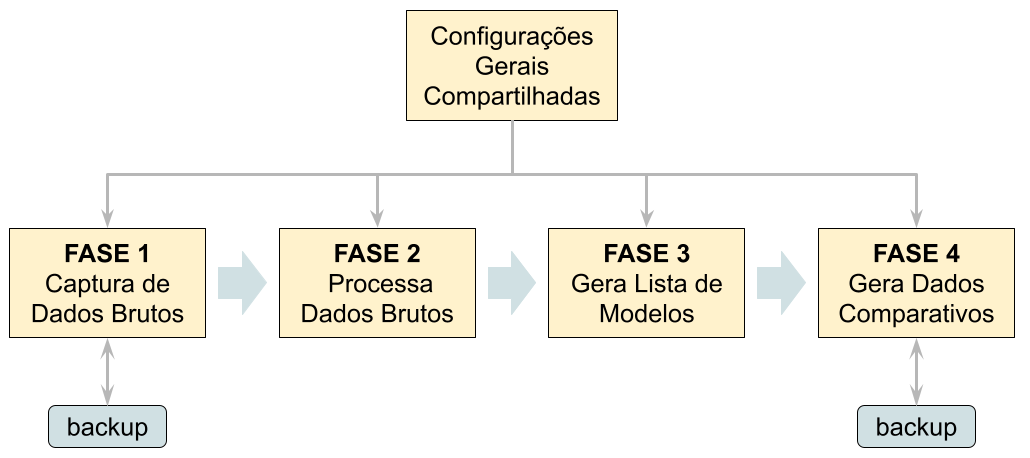
\includegraphics[width=\textwidth]{FIGURES/fig_25.png}
    \caption{Representação em alto nível do fluxo de execução do \textit{pipeline} de processamento. Fonte: Elaborada pelo autor.}
    \label{fig:25}
\end{figure}

Após a configuração geral do experimento e dos softwares, conforme descrito na seção \ref{cap:4.2}, o \textit{pipeline} automatiza a execução de todas as quatro fases. Nas Fases 1 e 4, um sistema de backup auxilia a retomada dos experimentos em caso de interrupção. A Fase 3 é responsável pela seleção do melhor modelo de aprendizado de máquina treinado com os dados gerados da Fase 2.

O algoritmo implementado no transcodificador rápido de VP9-para-AV1, e que será adaptado para os demais formatos considerados neste capítulo, será utilizado nas Fases 1, 2 e 4. Esse algoritmo será descrito com detalhes na seção \ref{cap:7.4}. Enquanto a seleção do melhor modelo de aprendizado de máquina (Fase 3) é descrita na seção \ref{cap:7.3}. O código-fonte do \textit{pipeline} proposto está disponível em \citet{bib:prototipotese}.

\subsection{Fase 1: Captura de Dados Brutos}
\label{cap:7.2.1}

É responsabilidade desta fase a captura dos dados brutos para treinamento e teste dos modelos de aprendizado de máquina. Os vídeos codificados no antigo formato são decodificados, gerando dois arquivos: o vídeo decodificado e os dados extraídos durante a decodificação. A partir do vídeo decodificado, a transcodificação é concluída com uma recodificação do conteúdo no novo formato, sem qualquer processo de aceleração, exportando um conjunto de dados. O fluxo de execução da Fase 1 é demonstrado na Figura \ref{fig:26}. Em todas as soluções apresentadas neste capítulo, o codificador utilizado foi o software \textit{libaom} do AV1. De forma geral, esta fase é responsável por:

\begin{enumerate}[1.]
    \item Decodificar o \textit{bitstream} pertencente ao conjunto de treinamento e de teste, que foi codificado em um formato pré-definido;

    \item Exportar informações provenientes do decodificador;

    \item Recodificar o vídeo decodificado para o novo formato, utilizando parâmetros de quantização pré-definidos;

    \item Exportar informações provenientes do codificador.
\end{enumerate}

\begin{figure}
    \centering
    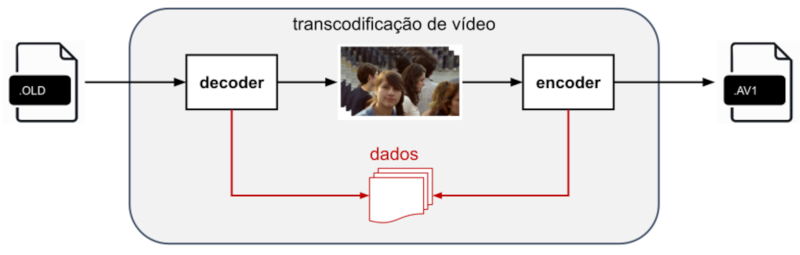
\includegraphics[width=0.85\textwidth]{FIGURES/fig_26.png}
    \caption{Representação da transcodificação realizada na Fase 1. Fonte: Elaborada pelo autor.}
    \label{fig:26}
\end{figure}


\subsection{Fase 2: Processamento de Dados Brutos}
\label{cap:7.2.2}

É responsabilidade desta fase o processamento dos dados brutos extraídos na primeira fase, de forma a gerar amostras passíveis de realizar corretamente o treinamento e o teste dos modelos treinados por aprendizado de máquina. Apesar de o processamento geral dos dados feito aqui também ser executado na fase 4, há uma significativa diferença entre ambos: na fase 4, toda a execução é feita internamente ao software codificador, enquanto aqui o processamento é executado externamente. Além disto, nesta segunda fase, também são processadas as decisões realizadas pelo codificador, a separação de conjuntos de dados em subconjuntos para cada modelo e o balanceamento de dados. Mais informações sobre os subconjuntos serão apresentadas na seção \ref{cap:7.3}. De forma geral, esta fase é responsável por:

\begin{enumerate}[1.]
    \item Unificar os dados extraídos na Fase 1, sob diferentes níveis de quantização;

    \item Remover elementos inválidos, existentes no conjunto de dados brutos;

    \item Dividir o conjunto de dados em subconjuntos de dados;

    \item Identificar os rótulos (decisões) para cada subconjunto;

    \item Balancear os dados;

    \item Exportar os dados balanceados em arquivos para treinamento e teste de cada modelo, conforme definido na seção \ref{cap:7.3}.
\end{enumerate}

Na responsabilidade 2, listada acima, acontece a remoção de elementos inválidos, pois, como veremos na seção \ref{cap:7.4}, regiões de borda do vídeo não são visíveis na imagem e, portanto, não podem gerar amostras passíveis de serem preditas pelo modelo de aprendizado de máquina.

O rótulo utilizado na proposta de transcodificador rápido deste capítulo é o subparticionamento do bloco atual em processamento, como melhor será abordado na seção \ref{cap:7.4}. Portanto, a identificação do rótulo (responsabilidade 4) é obtida com a observação das estruturas de particionamento existentes: caso o atual nível de profundidade seja subparticionado, então o rótulo é positivo (particiona), caso contrário, negativo (não particiona).

Como vimos no capítulo \ref{cap:5}, existe um desbalanceamento de ocorrência de particionamento de acordo com o nível de profundidade da árvore. Portanto, o balanceamento das amostras válidas é necessário para possibilitar o treinamento de modelos de forma mais correta. Nas soluções apresentadas nesta tese, optamos por balancear os dados em 50\%-50\%, ou seja, manter aproximadamente o mesmo número de exemplos com o rótulo positivo e com o rótulo negativo para cada subconjunto de amostras criado.

Existem duas principais técnicas de balanceamento de dados \cite{bib:livroRaschka}: \textbf{\textit{undersampling}}, onde remove-se amostras do rótulo majoritário e \textbf{\textit{oversampling}}, onde aumenta-se a representatividade dos dados do rótulo minoritário. Apesar de ambas apresentarem prós e contras, em geral as duas ocasionam um aumento no viés dos dados, seja por remover amostras importantes no treinamento, seja por ocasionar um sobreajuste dos dados, ou seja, gerar um modelo inviável para lidar com novos dados. Embora haja uma vasta literatura sobre como lidar com dados desbalanceados, como pode ser visto em \citet{bib:livroimbalanced}, não existe uma forma consolidada para automatizar o processo de análise de balanceamento de dados. Ou seja, ainda não é possível excluir o fator humano no processo de escolha do melhor balanceamento a ser aplicado nos dados, pois há a necessidade de avaliar os resultados e contexto de aplicação do modelo preditivo. Logo, optamos pela técnica de \textit{undersampling} através da remoção aleatória de amostras do conjunto majoritário. Para garantir a adaptabilidade desse processo, uma semente geradora de números aleatórios de valor 42 foi utilizada. 

\subsection{Fase 3: Geração de Lista de Modelos Preditivos}
\label{cap:7.2.3}

É responsabilidade desta fase o treinamento e o teste de todos os modelos preditivos gerados por algoritmos de aprendizado de máquina, além da seleção do melhor modelo para ser utilizado na fase de predição dos resultados. É com a combinação das configurações dos hiperparâmetros a serem utilizados (vide Tabela \ref{tab:XVIII}) que se obtém a lista completa de candidatos a serem treinados e testados. Neste processo, consideramos um universo de 9.526.572 candidatos de modelos de aprendizado de máquina para o algoritmo de árvore de decisão CART. Apesar disso, a modificação dos candidatos ou do próprio algoritmo de aprendizado de máquina é simples e não altera os demais fluxos automatizados do \textit{pipeline} de processamento.

É na seção \ref{cap:7.3} que iremos abordar com maiores detalhes os modelos treinados, contudo, para melhor compreensão desta subseção, se faz necessário a apresentação de alguns termos e informações. Na proposta de transcodificador rápido com uso de modelos preditivos, realizado nesta tese, iremos utilizar um grupo de modelos preditivos que trabalharão em conjunto, cada um responsável por predizer o rótulo sob condições específicas. Mais precisamente, há um modelo treinado para cada nível de profundidade da árvore do AV1, sob diferentes níveis de quantização. Dessa forma, como descreveremos melhor na seção \ref{cap:7.3}, há 12 modelos nesse conjunto, todos eles treinados sob o mesmo candidato de combinação de hiperparâmetros.

Dessa forma, a escolha pelo melhor candidato é feita através de uma competição iterativa entre os candidatos. Partindo-se de uma quantidade limitada e pequena de amostras, cada iteração dobra essa quantidade de amostras e, ao mesmo tempo, reduz pela metade o número de candidatos. Com isso, avaliamos todos os candidatos sob as mesmas condições e, após alguns ciclos iterativos e aceitando algum nível de incerteza, chega-se a ao melhor candidato. De forma geral, esta fase é responsável por:

\begin{enumerate}[1.]
    \item Gerar uma lista de candidatos a serem avaliados, com base no produto das variações dos hiperparâmetros;

    \item Avaliar todos os candidatos para cada um dos 12 modelos do grupo de modelos. De cada modelo treinado, selecionar os melhores 20 candidatos;

    \item Treinar o grupo de modelos com cada um dos candidatos de hiperparâmetros, com o conjunto completos de dados;

    \item Testar todos os modelos treinados com o conjunto de dados de teste;

    \item Reprovar modelos cujo AUC for inferior ao limite mínimo estabelecido na seção \ref{cap:7.3};

    \item Remover candidatos de hiperparâmetros que não tiverem todos os modelos aprovados;

    \item Calcular média de \textit{F1-Score} para todos os candidatos aprovados e ordená-los em ordem decrescente;

    \item Indicar para o restante do fluxo do \textit{pipeline} qual foi o candidato vencedor.
\end{enumerate}

\subsection{Fase 4: Geração de Dados Comparativos}
\label{cap:7.2.4}

É responsabilidade desta fase a geração dos dados comparativos entre a transcodificação rápida com uso dos modelos preditivos gerados por algoritmo de aprendizado de máquina, treinados com o candidato vencedor da Fase 3, em relação à transcodificação original. Nesta fase, são executadas as duas transcodificações e, consequentemente, sendo a fase mais custosa do \textit{pipeline}. De forma geral, esta fase é responsável por:

\begin{enumerate}[1.]
    \item Decodificar o \textit{bitstream} do conjunto de predição, que foi previamente codificado em algum formato pré-definido;

    \item Exportar informações provenientes do decodificador;

    \item Recodificar o vídeo decodificado para o novo formato, utilizando os níveis de quantização pré-definidos, utilizando a transcodificação original;

    \item Recodificar o vídeo decodificado para o novo formato, utilizando os níveis de quantização pré-definidos, utilizando a nossa proposta de transcodificador rápido;

    \item Exportar dados de transcodificação para permitir uma comparação objetiva.
\end{enumerate}

\section{Seleção dos Modelos de Aprendizado de Máquina}
\label{cap:7.3}

Como já vimos, a estrutura de particionamento de blocos do formato AV1 é composta por uma árvore que pode atingir até o sexto nível de profundidade. O particionamento de algum nível de profundidade em quatro novos ramos pode ser feito somente nos cinco primeiros níveis, conforme discutido no capítulo \ref{cap:5}. Naquele capítulo, inclusive, abordamos a distribuição da aplicação do particionamento para cada nível de profundidade e, como pudemos constatar, o software de referência do codificador AV1 opta pela divisão em quatro novos blocos de tamanho 8$\times$8 em apenas 16\% das vezes em que está processando a profundidade 3. Como visto no capítulo \ref{cap:5}, a opção por blocos iguais ou inferiores a 8$\times$8, em vídeos HD1080, se aproxima de no máximo 5\% no vídeo. Inclusive, a desativação nativa da profundidade 5 em vídeos de resolução UHD faz com que esse percentual de área dedicada a blocos pequenos seja significativamente menor. Desta forma, o ganho de tempo em se acelerar a escolha de subparticionamento rápido em blocos 8$\times$8 e 16$\times$16 é mínimo. Assim, na proposta de transcodificador rápido desenvolvido neste capítulo, não iremos utilizar modelos preditivos para as profundidades 3 e 4. Todavia, há outros três níveis de particionamento cuja aceleração com uso de modelos de aprendizado de máquina pode ser vantajosa, sendo eles de 128$\times$128 para 64$\times$64, de 64$\times$64 para 32$\times$32 e de 32$\times$32 para 16$\times$16.

Em vista desse fato, combinando o número de níveis de quantização utilizados utilizados nos experimentos apresentados nesta tese (quatro valores, como apresentamos no capítulo \ref{cap:4}) mais as três profundidades consideradas para decisão de particionamento, obtém-se um total de 12 conjuntos de amostras para treinamento, conforme listados abaixo:

\begin{itemize}
    \item Conjunto 1: CQ 20, particionamento de 128$\times$128 em 64$\times$64;

    \item Conjunto 2: CQ 20, particionamento de 64$\times$64 em 32$\times$32;

    \item Conjunto 3: CQ 20, particionamento de 32$\times$32 em 16$\times$16;

    \item Conjunto 4: CQ 32, particionamento de 128$\times$128 em 64$\times$64;

    \item Conjunto 5: CQ 32, particionamento de 64$\times$64 em 32$\times$32;

    \item Conjunto 6: CQ 32, particionamento de 32$\times$32 em 16$\times$16;

    \item Conjunto 7: CQ 43, particionamento de 128$\times$128 em 64$\times$64;

    \item Conjunto 8: CQ 43, particionamento de 64$\times$64 em 32$\times$32;

    \item Conjunto 9: CQ 43, particionamento de 32$\times$32 em 16$\times$16;

    \item Conjunto 10: CQ 55, particionamento de 128$\times$128 em 64$\times$64;

    \item Conjunto 11: CQ 55, particionamento de 64$\times$64 em 32$\times$32;

    \item Conjunto 12: CQ 55, particionamento de 32$\times$32 em 16$\times$16;
\end{itemize}

Com o objetivo de simplificar o balanceamento dos dados brutos a fim de permitir uma automatização mais direta das fases de treinamento e teste dos modelos, como apresentamos na subseção \ref{cap:7.2.2}, optamos por um balanceamento de 50\%-50\%, ou seja, cada rótulo dos dados de treinamento e de teste é representado a mesma quantidade de vezes no conjunto de amostras. Algum balanceamento dos dados se faz necessário, pois como visto no capítulo \ref{cap:5}, só no CQ 55, o primeiro nível de profundidade tende a se subparticionar em 99,42\% das vezes. Logo, havendo 99,42\% das amostras com rótulos positivo (isto é, particionar) e 0,58\% das amostras com rótulo negativo (isto é, não particionar), justifica-se a aplicação de algum balanceamento de dados, principalmente considerando que há 12 conjuntos diferentes de dados de treinamento.

\citet{bib:livroimbalanced} apresenta várias técnicas de balanceamento de dados e qualquer uma delas irá incluir algum tipo de viés nos dados, nos quais dois são os principais: \textit{oversampling} e \textit{undersampling}. Segundo o autor, a técnica de \textit{oversampling} pode aumentar a probabilidade de gerar um modelo preditivo com sobreajuste dos dados, uma vez que faz cópias das amostras da classe minoritária para se equivaler em número aos da classe majoritária. Desta forma, um modelo sobreajustado pode apresentar resultados estatísticos que são aparentemente precisos, mas na verdade só respondem bem a casos conhecidos e não são bons em predizer casos inéditos. Por outro lado, a técnica de \textit{undersampling} descarta uma quantidade significativa de amostras, e isso é problemático, pois a perda de tais amostras pode dificultar o aprendizado do modelo para casos que estejam no limite de decisão entre as instâncias minoritária e majoritária, resultando em uma perda no desempenho da classificação. Considerando essas observações de \citet{bib:livroimbalanced} mais a desproporção dos desbalanceamentos observados, ponderamos que adaptar 0,58\% dos dados para se equivaler a 99,42\% dos demais rótulos não é eficiente. Assim, optamos por utilizar a técnica de balanceamento de dados com \textit{undersampling} aleatório.

É possível obter uma relação da quantidade máximas e teóricas dos dados de treinamento, a despeito do seu desbalanceamento, pois esses valores são diretamente proporcionais à quantidade de vídeos utilizados, de sua resolução e da quantidade de quadros utilizados na codificação. Dessa forma, considerando os vídeos de treinamento expostos na seção \ref{cap:7.1}, a quantidade máxima de amostras para cada rótulo que podemos obter para cada profundidade é de 47.040 (para profundidade 0), 194.880 (profundidade 1) e 817.740 (profundidade 2). No entanto, essas amostras estão desbalanceadas. Portanto, após realizar o processo de balanceamento exposto no parágrafo anterior, obtemos o número de amostras para cada rótulo apresentadas nas Tabelas \ref{tab:XIX}, \ref{tab:XX}, \ref{tab:XXI}, \ref{tab:XXII} e \ref{tab:XXIII} para as transcodificações VP8-AV1, VP9-AV1, H.264/AVC-AV1, H.265/HEVC-AV1 e H.266/VVC-AV1, respectivamente. Nessas tabelas, também são apresentadas a quantidade de amostras para os conjuntos de testes.

\begin{table}
\begin{center}
\caption{Quantidade de amostras de treinamento e teste de modelos preditivos para a transcodificação VP8-AV1 após o balanceamento.}
\label{tab:XIX}
\footnotesize

\begin{tblr}{
    colspec = {l|l|r|r|r},
    hlines,
    row{even} = {gray9},
    cell{5}{1} = {gray9},
    cell{9}{1} = {gray9}
}
\hline
\SetCell[c=2]{c} && \SetCell[c=3]{c}\textbf{Profundidade}    \\
\textbf{CQ}                  & \textbf{Conjunto de} & \textbf{0 (128$\times$128)} & \textbf{1 (64$\times$64)} & \textbf{2 (32$\times$32)} \\
\SetCell[r=2]{c}20 & treinamento & 29.485      & 115.893   & 238.375   \\
                   & teste       & 29.487      & 114.063   & 188.627   \\
\SetCell[r=2]{c}32 & treinamento & 35.385      & 119.601   & 229.431   \\
                   & teste       & 31.595      & 101.505   & 164.651   \\
\SetCell[r=2]{c}43 & treinamento & 36.951      & 109.673   & 183.869   \\
                   & teste       & 31.741      & 78.815    & 121.035   \\
\SetCell[r=2]{c}55 & treinamento & 37.093      & 91.247    & 123.445   \\
                   & teste       & 31.913      & 65.897    & 68.029   \\

\hline
\end{tblr}
\end{center}
\end{table}

\begin{table}
\begin{center}
\caption{Quantidade de amostras de treinamento e teste de modelos preditivos para a transcodificação VP9-AV1 após o balanceamento.}
\label{tab:XX}
\footnotesize

\begin{tblr}{
    colspec = {l|l|r|r|r},
    hlines,
    row{even} = {gray9},
    cell{5}{1} = {gray9},
    cell{9}{1} = {gray9}
}
\hline
\SetCell[c=2]{c} && \SetCell[c=3]{c}\textbf{Profundidade}    \\
\textbf{CQ}                  & \textbf{Conjunto de} & \textbf{0 (128$\times$128)} & \textbf{1 (64$\times$64)} & \textbf{2 (32$\times$32)} \\
\SetCell[r=2]{c}20 & treinamento & 38.537 & 133.935 & 251.863   \\
                   & teste       & 30.941 & 89.017 & 145.783   \\
\SetCell[r=2]{c}32 & treinamento & 42.191 & 132.475 & 232.079   \\
                   & teste       & 37.055 & 87.115 & 171.525   \\
\SetCell[r=2]{c}43 & treinamento & 42.293 & 125.575 & 184.545   \\
                   & teste       & 37.201 & 758.95 & 121.567   \\
\SetCell[r=2]{c}55 & treinamento & 42.443 & 107.471 & 120.343   \\
                   & teste       & 37.337 & 66.111 & 62.661   \\

\hline
\end{tblr}
\end{center}
\end{table}

\begin{table}
\begin{center}
\caption{Quantidade de amostras de treinamento e teste de modelos preditivos para a transcodificação H.264/AVC-AV1 após o balanceamento.}
\label{tab:XXI}
\footnotesize

\begin{tblr}{
    colspec = {l|l|r|r|r},
    hlines,
    row{even} = {gray9},
    cell{5}{1} = {gray9},
    cell{9}{1} = {gray9}
}
\hline
\SetCell[c=2]{c} && \SetCell[c=3]{c}\textbf{Profundidade}    \\
\textbf{CQ}                  & \textbf{Conjunto de} & \textbf{0 (128$\times$128)} & \textbf{1 (64$\times$64)} & \textbf{2 (32$\times$32)} \\
\SetCell[r=2]{c}20 & treinamento & 30.233 & 113.225 & 226.393   \\
                   & teste       & 32.107 & 120.487 & 190.105   \\
\SetCell[r=2]{c}32 & treinamento & 35.949 & 112.485 & 215.039   \\
                   & teste       & 36.943 & 110.657 & 171.583   \\
\SetCell[r=2]{c}43 & treinamento & 37.015 & 103.269 & 172.291   \\
                   & teste       & 37.157 & 78.757 & 118.595   \\
\SetCell[r=2]{c}55 & treinamento & 37.127 & 91.473 & 112.135   \\
                   & teste       & 37.321 & 65.807 & 56.141   \\

\hline
\end{tblr}
\end{center}
\end{table}

\begin{table}
\begin{center}
\caption{Quantidade de amostras de treinamento e teste de modelos preditivos para a transcodificação H.265/HEVC-AV1 após o balanceamento.}
\label{tab:XXII}
\footnotesize

\begin{tblr}{
    colspec = {l|l|r|r|r},
    hlines,
    row{even} = {gray9},
    cell{5}{1} = {gray9},
    cell{9}{1} = {gray9}
}
\hline
\SetCell[c=2]{c} && \SetCell[c=3]{c}\textbf{Profundidade}    \\
\textbf{CQ}                  & \textbf{Conjunto de} & \textbf{0 (128$\times$128)} & \textbf{1 (64$\times$64)} & \textbf{2 (32$\times$32)} \\
\SetCell[r=2]{c}20 & treinamento & 34.025 & 114.627 & 232.023   \\
                   & teste       & 21.287 & 60.171 & 125.563   \\
\SetCell[r=2]{c}32 & treinamento & 28.883 & 86.755 & 163.465   \\
                   & teste       & 20.879 & 47.105 & 111.405   \\
\SetCell[r=2]{c}43 & treinamento & 27.771 & 81.985 & 137.667   \\
                   & teste       & 31.823 & 73.165 & 126.757   \\
\SetCell[r=2]{c}55 & treinamento & 21.307 & 62.815 & 80.835   \\
                   & teste       & 15.893 & 46.909 & 40.937   \\

\hline
\end{tblr}
\end{center}
\end{table}

\begin{table}
\begin{center}
\caption{Quantidade de amostras de treinamento e teste de modelos preditivos para a transcodificação H.266/VVC-AV1 após o balanceamento.}
\label{tab:XXIII}
\footnotesize

\begin{tblr}{
    colspec = {l|l|r|r|r},
    hlines,
    row{even} = {gray9},
    cell{5}{1} = {gray9},
    cell{9}{1} = {gray9}
}
\hline
\SetCell[c=2]{c} && \SetCell[c=3]{c}\textbf{Profundidade}    \\
\textbf{CQ}                  & \textbf{Conjunto de} & \textbf{0 (128$\times$128)} & \textbf{1 (64$\times$64)} & \textbf{2 (32$\times$32)} \\
\SetCell[r=2]{c}20 & treinamento & 35.405 & 125.719 & 147.691\\
                   & teste       & 36.579 & 123.265 & 86.685\\
\SetCell[r=2]{c}32 & treinamento & 36.935 & 116.395 & 206.447\\
                   & teste       & 37.031 & 97.013 & 141.231\\
\SetCell[r=2]{c}43 & treinamento & 36.981 & 106.637 & 172.987\\
                   & teste       & 37.181 & 78.023 & 102.277\\
\SetCell[r=2]{c}55 & treinamento & 37.099 & 95.047 & 112.299\\
                   & teste       & 37.313 & 68.183 & 54.689\\

\hline
\end{tblr}
\end{center}
\end{table}


Na subseção \ref{cap:7.1.3}, citamos que são considerados 9.526.572 combinações candidatas de hiperparâmetros para o algoritmo de aprendizado de máquina CART \cite{bib:livroCART}. É necessário selecionar o melhor candidato dentre todos, a fim de submeter esse candidato à Fase 4 do \textit{pipeline}. A forma mais justa de descobrir qual deles apresenta o melhor resultado de \textit{F1-Score} é realizar o treinamento completo com todos os candidatos e obter a média estatística de cada um desses modelos, após a rodada de testes. No entanto, a aplicação da técnica de busca exaustiva para encontrar o melhor modelo não é viável em termos de tempo de processamento. Apesar de cada combinação de hiperparâmetros apresentar um tempo de treinamento relativamente fixo de apenas seis segundos para o conjunto com maiores amostras (profundidade 2 e CQ 20, conforme Tabela \ref{tab:XX}), ao considerarmos o universo completo de combinações (de 9.526.572), o treinamento em busca exaustiva para todos os 12 modelos seria finalizado em 21,8 anos.

Desse modo, é fundamental que se aplique alguma metodologia de treinamento rápido a fim de providenciar um candidato vencedor em tempo hábil. Há diversas formas discutidas na literatura para lidar com esse problema, cada uma com suas características positivas e negativas, sendo que a resolução desse problema, inclusive, é uma área de forte interesse na academia. Uma das técnicas mais conhecidas envolve a busca por grade \cite{bib:randomsearch} (do inglês, \textit{Grid Search}), onde devem ser definidos os valores de cada hiperparâmetro que se deseja testar e, em seguida, todas as combinações possíveis desses valores serão testadas. No entanto, essa técnica é muito custosa, caso existam muitos valores a serem testados. Por outro lado, principalmente visando acelerar a busca por hiperparâmetros, também pode ser encontrada na literatura a técnica de busca por grade aleatória (do inglês, \textit{Random Grid Search}, RGS). Nesta técnica, os valores a serem testados para cada hiperparâmetro são definidos pelo par de limites: inferior e superior. Desta forma, valores aleatórios dentro desse intervalo-limite são testados e avaliados, podendo-se dar maior exploração de busca em sub-intervalos cujos resultados sejam mais apurados.

Contudo, apesar da técnica RGS ser mais eficiente em termos de uso de recursos computacionais do que a técnica de busca por grade simples, uma série de candidatos não são testados, o que pode ocasionar em encontrar combinações que sejam categorizados como máximos locais. Ou seja, existe uma possibilidade de não serem encontrados os máximos globais. Dessa forma, optamos por utilizar outra técnica de avaliação de hiperparâmetros que permite avaliar todas as suas combinações, tornando possível aproximar o resultado de máximos globais e, ainda assim, ter um tempo de processamento rápido: a busca por hiperparâmetros com validação cruzada e com cortes randomizados e recursivos \cite{bib:halvingrandomsearch}, do inglês, \textit{Halving Random Search with Cross Validation} (HRSCV).

A Figura \ref{fig:29} exemplifica o funcionamento da HRSCV, na qual cada ciclo corresponde a três fases de processamento: seleção, treinamento/teste e avaliação. No entanto, em vez de processar treinamentos com o conjunto completo de amostras, como ocorre com a busca exaustiva ou a RGS, a HRSCV seleciona aleatoriamente uma parte das amostras e realiza o treinamento de todas as combinações de hiperparâmetros por meio de uma validação cruzada com cinco subconjuntos mutuamente exclusivos. A etapa de seleção de amostras é importante, pois, a cada novo ciclo, a HRSCV seleciona mais amostras disponíveis no conjunto, a um crescimento definido por $fator$. Essa variável, $fator$, é determinante para definir o crescimento do custo computacional empregado na HRSCV. Iniciando com um conjunto de tamanho definido pelo usuário (preferencialmente múltiplo de cinco), cada nova iteração da HRSCV aumenta o tamanho da amostra em $fator$ vezes, ao mesmo tempo que o número de combinações de hiperparâmetros decai em $fator$ vezes. Portanto, apesar de tecnicamente o produto entre combinações de hiperparâmetros e o tamanho da amostra de treinamento ser o mesmo ao longo dos ciclos, o custo computacional de treinar um modelo com cada vez mais amostras é maior. Dessa forma, a HRSCV garante um treinamento significativamente rápido no primeiro ciclo, mesmo considerando um conjunto grande de combinações de hiperparâmetros, por dispor de um número ínfimo de amostras. A cada novo ciclo, aumentamos o custo computacional para treinamento e, ao mesmo tempo, ganhamos maior confiança nos resultados obtidos com os testes. Por essa razão, o custo computacional da HRSCV é diretamente proporcional aos valores definidos (tamanho da amostra inicial, $fator$ e número de combinações de hiperparâmetros), podendo apresentar custos superiores ao de uma técnica de busca exaustiva, caso os valores definidos não forem ajustados de acordo com as necessidades.

\begin{figure}
    \centering
    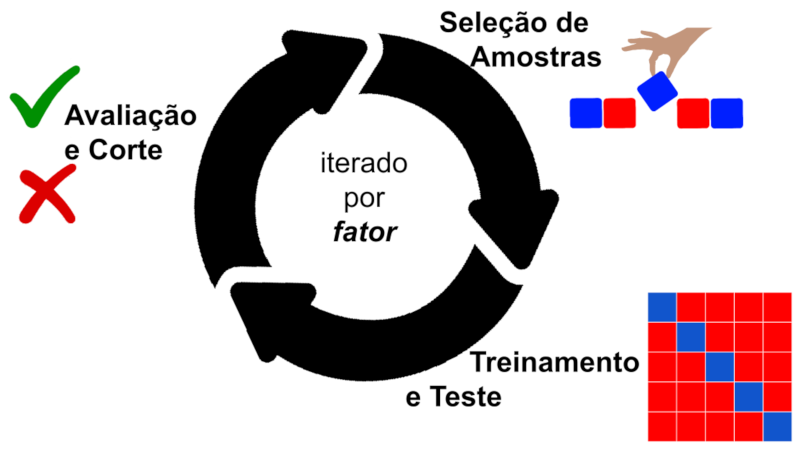
\includegraphics[width=0.5\textwidth]{FIGURES/fig_29.png}
    \caption{Fluxo geral de execução da técnica de avaliação de hiperparâmetros \textit{Halving Random Search with Cross Validation}. Fonte: Elaborada pelo autor.}
    \label{fig:29}
\end{figure}

Uma das formas que a HRSCV possui para limitar o seu custo computacional é definir as condições de parada de sua execução, sendo elas: (a) não haver mais combinações de hiperparâmetros a serem comparados e (b) não haver mais amostras suficientes para iniciar um novo ciclo. A primeira condição, basicamente, indica que foi encontrado o melhor modelo dentro de todas as combinações de hiperparâmetros. Já a segunda condição sinaliza que não há um conjunto de amostras com o tamanho necessário para iniciar o ciclo, sendo finalizada a HRSCV contendo não o vencedor, mas uma lista de N melhores combinações de hiperparâmetros até o momento, em ordem decrescente de pontuação. Conforme já definimos anteriormente, as propostas deste capítulo utilizam como métrica para esta pontuação o valor de \textit{F1-Score}.

Expostas essas informações, é possível estimar quantos ciclos de execução são executados, com base nos valores iniciais da técnica HRSCV, cujos valores de combinações e amostras são, respectivamente, calculados pelas equações \ref{eq:9} e \ref{eq:10}. O tamanho de combinações de hiperparâmetros inicial já é conhecido (9.526.572) e o valor de $fator$ deve ser adequado ao problema, mas obrigatoriamente maior que 1. Vamos manter o tamanho de $fator$ padrão, que é de 2, ou seja, a cada ciclo, o número de combinações cai pela metade enquanto o tamanho da amostra dobra. Por fim, devemos definir a quantidade de amostras que são utilizadas no primeiro ciclo da HRSCV. Em sua documentação em \citet{bib:halvingrandomsearch}, o recomendado é que este valor seja no mínimo cinco vezes $fator$ amostras por número de atributos usados para treinar o modelo. Como veremos na seção \ref{cap:7.4}, são utilizados 25 atributos para treinamento dos modelos; logo, o recomendado é utilizar ao menos 250 amostras no primeiro ciclo.

\begin{equation}
    \label{eq:9}
    Amostras_{ciclo}=Amostras_{inicial}*fator^{ciclo - 1}
\end{equation}

\begin{equation}
    \label{eq:10}
    Combinacoes_{ciclo}=Combinacoes_{inicial}*fator^{ciclo - 1}
\end{equation}

Conhecendo as condições de início da HRSCV aplicadas para geração dos modelos propostos, é possível estimar quantos ciclos seriam executados para cada um dos subconjuntos de treinamento, conforme explicitados na Tabela \ref{tab:XXIV}. Nesta tabela, apresentamos todos os ciclos possíveis até atingir a condição de parada (a), ou seja, de encontrar a melhor combinação de hiperparâmetros. Todavia, não temos um conjunto de treinamento que contenha dois bilhões de amostras, como exigiria o 24$^\circ$ ciclo apresentado na Tabela \ref{tab:XXIV}. Ainda assim, evidenciamos que o menor conjunto de treinamento (profundidade 0 para o CQ 55, conforme Tabela \ref{tab:XXII}), pode ser processado em oito ciclos, retornando uma lista com mais de 37 mil combinações de hiperparâmetros. Já o maior conjunto de treinamento (da profundidade 2 para o CQ 20), pode ser processado em 11 ciclos, retornando uma lista com 9 mil combinações de hiperparâmetros.

\begin{table}
\begin{center}
\caption{Número de candidatos e amostras necessárias para execução de cada ciclo da técnica HRSCV, conforme condições definidas nesta tese.}
\label{tab:XXIV}
\footnotesize

\begin{tblr}{
    colspec = {l|r|r},
    hlines,
    row{even} = {gray9}
}
\hline

\textbf{Ciclo} & \textbf{Candidatos} & \textbf{Amostras}      \\
1     & 9.526.572  & 250           \\
2     & 4.763.286  & 500           \\
3     & 2.381.643  & 1.000         \\
4     & 1.190.822  & 2.000         \\
5     & 595.411    & 4.000         \\
6     & 297.705    & 8.000         \\
7     & 148.853    & 16.000        \\
8     & 74.426     & 32.000        \\
9     & 37.213     & 64.000        \\
10    & 18.607     & 128.000       \\
11    & 9.303      & 256.000       \\
12    & 4.652      & 512.000       \\
13    & 2.326      & 1.024.000     \\
14    & 1.163      & 2.048.000     \\
15    & 581        & 4.096.000     \\
16    & 291        & 8.192.000     \\
17    & 145        & 16.384.000    \\
18    & 73         & 32.768.000    \\
19    & 36         & 65.536.000    \\
20    & 18         & 131.072.000   \\
21    & 9          & 262.144.000   \\
22    & 5          & 524.288.000   \\
23    & 2          & 1.048.576.000 \\
24    & 1          & 2.097.152.000 \\
\hline
\end{tblr}
\end{center}
\end{table}


De cada uma dessas 12 listas retornadas ao fim da execução da HRSCV, capturamos os 20 melhores, unificando-os para obter uma lista de até 240 combinações de hiperparâmetros. há a possibilidade de existirem combinações repetidas nas listas, logo, as repetições são eliminadas. Só então, aplicamos o treinamento e o teste completo para os modelos, de forma a gerar uma lista com dados estatísticos de todos esses candidatos. Com esses processos de filtragem, reduzimos o tempo de processamento de 21 anos de uma busca exaustiva para menos de 10 horas.

Em posse da lista dos 240 candidatos e dos seus valores estatísticos, removemos todos os que não atingem ao menos 0,75 pontos de AUC, mesmo que para apenas um único modelo. Como a AUC informa a probabilidade de o modelo retornar uma resposta positiva corretamente, determinamos que o mínimo valor aceitável seja de 0,75, por ser a metade entre o pior (0,5) e o melhor (1,0) AUC possível. Após essa filtragem final, calculamos a média do \textit{F1-Score} de todos os modelos que foram treinados sob uma mesma combinação de hiperparâmetros, ordenando-os por valor de \textit{F1-Score} médio. Aquele candidato que estiver em primeiro lugar nesta lista, será utilizado na Fase 4 do \textit{pipeline}, a fim de ser aplicado na aceleração da transcodificação.

\section{Transcodificação Rápida para o AV1}
\label{cap:7.4}

Nesta seção, apresentamos as modificações realizadas nos diversos decodificadores e no codificador de referência do AV1 para permitir o desenvolvimento da transcodificação rápida proposta neste capítulo, indicando pontos que são compartilhados em diversas fases de execução do \textit{pipeline} proposto. Para possibilitar uma apresentação mais clara, o conteúdo encontra-se dividido em dois pontos: proposta de algoritmo de transcodificação rápida (subseção \ref{cap:7.4.1}) e modificações necessárias para adequar os decodificadores ao algoritmo desenvolvido de transcodificação rápida (subseção \ref{cap:7.4.2}).

\subsection{Proposta de Algoritmo de Transcodificação Rápida}
\label{cap:7.4.1}

Antes de apresentar a nossa proposta, se faz necessário compreender o fluxo de execução do algoritmo de particionamento de blocos do software de referência do AV1, em sua versão 3.5.0, representado na Figura \ref{fig:30}. Nesta figura, observam-se quatro conjuntos principais de processos: 

\begin{itemize}
    \item \textbf{Blocos verdes}, indicando de início e fim de processos;

    \item \textbf{Blocos cinzas}, indicando processos de predição intraquadro ou interquadros nos blocos daquele tipo de particionamento;

    \item \textbf{Blocos azuis}, indicando processos de podas antecipadas realizadas através de modelos preditivos nativos do \textit{libaom};

    \item \textbf{Bloco branco}, indicando um condicional que avalia se as podas realizadas não geraram situação impossível, por exemplo, uma repetição infinita ou uma impossibilidade de obter melhores resultados de custo taxa-distorção (rd-cost).
\end{itemize}

\begin{figure}
    \centering
    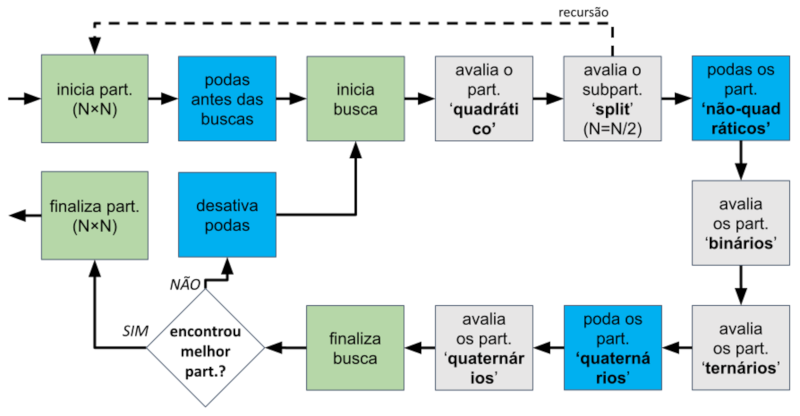
\includegraphics[width=0.75\textwidth]{FIGURES/fig_30.png}
    \caption{Diagrama de execução da busca da melhor estrutura de particionamentos no \textit{libaom} 3.5.0. Fonte: Elaborada pelo autor.}
    \label{fig:30}
\end{figure}

Há uma recursão explícita no fluxo de particionamento de blocos do AV1, conforme pode ser observado na Figura \ref{fig:30}. Recursão essa que é aplicada para quatro novos processos, cada um relacionado a um novo ramo da árvore de particionamentos. Nas versões anteriores do \textit{libaom}, era obrigatório o teste de predição intraquadro ou interquadros no bloco em processamento com ao menos um modo de predição, o que explica a obrigatoriedade da predição simples aplicada ao nosso trabalho de H.265/HEVC-para-AV1 na seção \ref{cap:6.1}. Contudo, na versão atual do \textit{libaom}, é possível ignorar a predição, caso o processo de podas realizado antes das buscas assim identifique. Neste caso, apenas o modo de particionamento \textit{SPLIT} é executado, ou seja, a recursão é aplicada.

Como já foi esclarecido, os modelos preditivos gerados na proposta de transcodificador rápido decidem sobre o particionamento ou não do bloco atual. Logo, modificamos o fluxo de execução do particionamento de blocos da Figura \ref{fig:30} para incluir os processos de antecipação do modo \textit{SPLIT}, realizado através dos modelos preditivos propostos neste capítulo, conforme pode ser visto em laranja na Figura \ref{fig:31}.

\begin{figure}
    \centering
    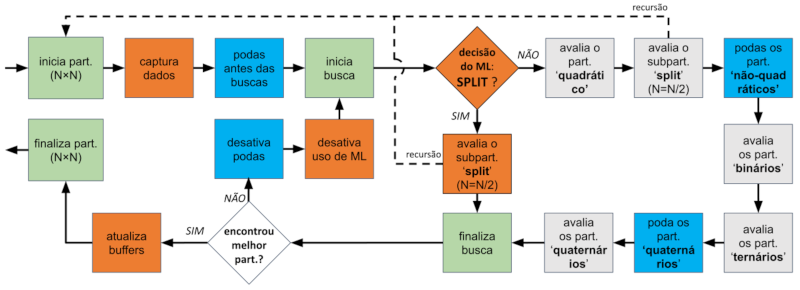
\includegraphics[width=\textwidth]{FIGURES/fig_31.png}
    \caption{Diagrama de execução da busca da melhor estrutura de particionamentos no transcodificador rápido (\textit{libaom} 3.5.0). Fonte: Elaborada pelo autor.}
    \label{fig:31}
\end{figure}

Na Figura \ref{fig:31} observam-se cinco modificações (destacados em laranja), cada uma responsável por um processo específico, conforme descrevemos abaixo:

\begin{enumerate}[1.]
    \item Selecionar informações nos \textit{buffers} que alimentam o modelo preditivo;

    \item Avaliar respostas dos modelos preditivos propostos;

    \item Utilizar o tipo de particionamento \textit{SPLIT}, caso os modelos propostos assim indiquem;

    \item Desativar o modelo de aprendizado de máquina proposto, caso o condicional do fluxo principal de execução do particionamento de blocos do \textit{libaom} assim o indique;

    \item Atualizar informações processadas aos \textit{buffers} que alimentam o modelo preditivo proposto.
\end{enumerate}

Dentre esses cinco processos implementados no fluxo de execução do particionamento de blocos, destacam-se dois: atualização de \textit{buffers} e captura de dados. O primeiro destes processos tem como objetivo ler as informações extraídas tanto do decodificador como do codificador e armazená-las em estruturas de dados que, durante o segundo destes processos, alimentará os modelos preditivos. É após a resposta positiva do condicional do fluxo de execução do particionamento de blocos que se torna possível a obtenção das decisões obtidas naquele nível de profundidade do AV1. Logo, a atualização das estruturas de dados que alimentam o modelo preditivo só ocorre neste momento, independente da profundidade processada. Os tipos de dados extraídos, tanto do decodificador como do codificador, são idênticos, pois dessa forma se reduz significativamente a complexidade de adaptação de estruturas de dados e modificações de tipos de dados ao adaptar o algoritmo de transcodificador rápido para outros formatos. Portanto, as seguintes variáveis são coletadas:

\begin{enumerate}[1.]
    \item \textbf{Nível de Profundidade}: indica quantas vezes a árvore de particionamento se dividiu. Essa variável está diretamente ligada ao rótulo a ser predito. Esperam-se valores inteiros e maiores que 0, onde 0 indica que o superbloco não se subdividiu (ou seja, um bloco quadrático equivalente a 128$\times$128). O valor máximo esperado é 5, onde a árvore atingiu a profundidade máxima, ou seja, bloco de tamanho 4$\times$4. Ressalta-se que atribuímos 0 para blocos 128$\times$128, pois este é o maior tamanho de bloco atualmente disponível nos formatos de codificação de vídeo;

    \item \textbf{Tamanho de bloco}: informa um código referente ao tamanho de bloco utilizado. É relevante utilizar essa variável em conjunto com a anterior porque, apesar de ser possível inferir a profundidade da árvore por meio do tamanho de bloco, o inverso não é verdade. Por exemplo, o bloco 32$\times$32 em essência está na profundidade 2, mas caso o AV1 utilize algum tipo de particionamento ternário (tipo \textit{AB}), esse mesmo tamanho de bloco estará, na verdade, na profundidade 1. São esperados valores inteiros, correspondentes à identificação interna do software do codificador para esses tamanhos de blocos;

    \item \textbf{Orientação dos blocos}: informa qual é a orientação dos blocos não quadráticos utilizados naquela profundidade. Essa variável complementa as duas variáveis anteriores, pois auxilia a identificar o tamanho do bloco com a profundidade. São esperados valores inteiros, onde 0 indica o uso de blocos quadráticos, código 1 indica orientação horizontal e código 2 indica orientação vertical; 

    \item \textbf{Modo de predição}: informa o código do modo de predição intraquadro ou interquadros utilizado pelo codificador;

    \item \textbf{Tipo de predição}: complementa a variável anterior, indicando qual foi o tipo de predição realizado, se intraquadro (código 0) ou interquadros (código 1). Essa variável é utilizada porque há uma tendência de blocos menores serem codificados com predição do tipo intraquadro, o que pode auxiliar o modelo a identificar possíveis subparticionamentos de blocos.
\end{enumerate}

No algoritmo de transcodificação rápido desenvolvido, sumarizado na Figura \ref{fig:31}, as informações que alimentam os modelos preditivos são capturadas e armazenadas em \textit{buffers}, que contêm todas as variáveis acima citadas de regiões vizinhas ao bloco em processamento (B.P.). A escolha por regiões vizinhas como fonte de informações para uso em modelos preditivos já foi observada em \citet{bib:guo_2018}, indicando que é particularmente mais eficiente em vídeos de resolução HD1080 ou superior. Desta forma, representamos na Figura \ref{fig:32} as regiões nas quais as variáveis acima citadas serão capturadas, a fim de alimentar o modelo preditivo. Nesta figura, observam-se cinco regiões (A, B, C, D e E) distantes N pixels da posição do B.P., nas quais serão capturados cinco valores de cada uma. Logo, os modelos preditivos utilizados nas soluções propostas neste capítulo utilizam 25 atributos para embasar as suas decisões. Observe que, por utilizarmos regiões vizinhas ao B.P., as regiões B, C, D e E, eventualmente, podem estar localizadas aquém dos limites do quadro, isto é, suas posições x e y podem ser menores que zero. Nesses casos excepcionais, os modelos preditivos estarão desabilitados para uso naquela iteração da busca da melhor estrutura de particionamentos no \textit{libaom}.

\begin{figure}
    \centering
    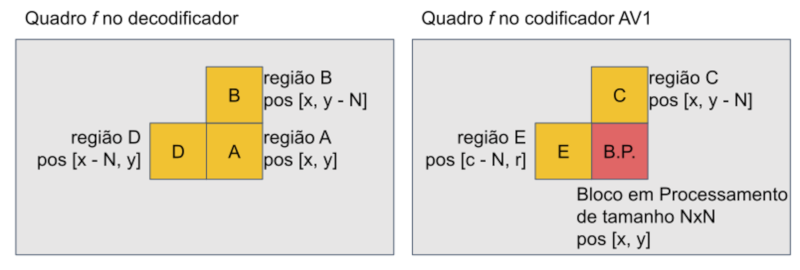
\includegraphics[width=0.75\textwidth]{FIGURES/fig_32.png}
    \caption{Representação em alto nível das regiões onde atributos são selecionados para alimentar o modelo preditivo. Fonte: Elaborada pelo autor.}
    \label{fig:32}
\end{figure}

Sete matrizes compõem as estruturas de dados utilizadas para armazenar as informações, sendo quatro dedicadas ao armazenamento das informações provenientes do decodificador, quatro para armazenar as decisões do codificador e uma matriz auxiliar (AUX) utilizada para preenchimento das seis matrizes anteriores. É nesta matriz AUX que serão armazenadas todas as informações observadas durante a decodificação e a re-codificação, em áreas de 4$\times$4 pixels e, desta forma, utilizadas para alimentar corretamente as outras matrizes. Cada uma das matrizes principais são utilizadas para o armazenamento de informações relativas ao nível de profundidade ao qual estão associadas. Conforme pode ser visto na Figura \ref{fig:33}, cada uma das matrizes principais possui um tamanho distinto e proporcional à resolução do vídeo, onde cada ponto (P) dessa matriz representa uma área de igual tamanho de bloco ao qual está sendo processado (128$\times$128, 64$\times$64 ou 32$\times$32). Assim, considerando um vídeo de resolução HD1080, a matriz com P igual a 128$\times$128 terá o tamanho de 15$\times$9. Ao final do processo ``\textit{Atualiza Buffers}'', apresentado na Figura \ref{fig:32}, a matriz auxiliar é utilizada para geração de médias que preencherão as matrizes principais.

\begin{figure}
    \centering
    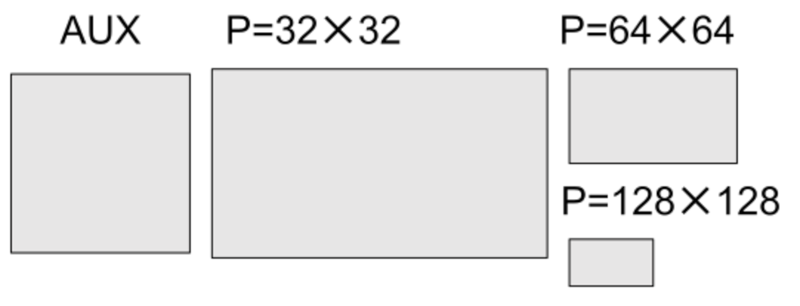
\includegraphics[width=0.5\textwidth]{FIGURES/fig_33.png}
    \caption{Representação do tamanho das matrizes utilizadas pelas estruturas de dados implementadas. Fonte: Elaborada pelo autor.}
    \label{fig:33}
\end{figure}

\subsection{Informações Extraídas dos Softwares Decodificadores}
\label{cap:7.4.2}

Na subseção anterior apresentamos o algoritmo proposto para transcodificação rápida para o formato AV1, cuja estrutura geral pode ser adaptada para demais propostas de transcodificador. Como discutido na subseção anterior, todas as regiões apresentadas na Figura \ref{fig:32} armazenam os mesmos tipos de informações. Logo, cada um dos decodificadores considerados precisam exportar as mesmas informações, na medida que isso seja possível. Nesta subseção, discutimos de que forma isso foi implementado.

Um dos dados exportados não versa sobre nenhuma das cinco variáveis necessárias para preenchimento das matrizes principais, mas identifica a posição do bloco ao qual correspondem as informações no quadro decodificado. Enquanto os padrões H.265/HEVC e H.266/VVC utilizam posições reais de pixels para identificar regiões do quadro, ou seja, um bloco na posição [384, 512] está de fato nesta posição no quadro, no padrão H.264/AVC e nos formatos VP8, VP9 e AV1, cada posição de bloco não é um valor absoluto de pixel, mas um referencial para o menor conjunto de blocos existente naquele formato. Dessa forma, a posição [384, 512] no formato AV1 indica um bloco localizado a partir do pixel [1536, 2048], por exemplo. Portanto, as posições de bloco representadas em cada decodificador precisam ser adequados para o formato utilizado pelo AV1, seguindo as regras abaixo:

\begin{itemize}
    \item Se a posição for originária de um vídeo no formato VP8 ou do padrão H.264/AVC, multiplicar os valores na tupla por quatro;

    \item Se a posição for originária de um vídeo no formato VP9, multiplicar os valores da tupla por dois;

    \item Se a posição for originária de um vídeo codificado nos padrões H.265/HEVC ou H.266/VVC, dividir os valores da tupla por quatro.
\end{itemize}

Já em relação à obtenção das variáveis propriamente ditas, as duas que não precisam ser adaptadas em nenhum dos cinco formatos utilizados na decodificação (VP8, VP9, H.264/AVC, H.265/HEVC e H.266/VVC) são as variáveis ``\textit{Orientação do Bloco}'' e ``\textit{Modo de Predição}''. No caso da primeira, basta observar os tamanhos de blocos utilizados; na segunda, exporta-se a informação sem nenhum de adaptação de valores, já que cada formato de codificação possui uma identificação numérica própria para esses modos de predição. Dessa forma, preferimos manter essa identificação inalterada. A variável ``\textit{Nível de Profundidade}'', como discutido na subseção anterior, contabiliza o número de vezes que o modo \textit{SPLIT} foi escolhido. No entanto, apenas o padrão H.266/VVC possui nível zero, por ser o único formato que oferece tamanho de bloco igual a 128$\times$128, além do AV1. Para todos os demais formatos, adaptou-se a contagem de particionamentos para torná-la equivalente à numeração observada no formato AV1. A única exceção recai para o VP8, que só possui dois tamanhos de blocos: 16$\times$16 e 4$\times$4; logo, há somente dois níveis de profundidades no VP8: 3 e 5.

Ainda no formato VP8, o tamanho de bloco utilizado já indica o tipo de predição realizado, isto é, se intraquadro (blocos 4$\times$4) ou interquadros (blocos 16$\times$16). Por outro lado, apesar dos formatos H.265/HEVC e H.266/VVC compartilharem a variável que indica se o tipo de predição é intraquadro ou interquadros, o tamanho de bloco não é fator decisivo para essa informação. Inclusive, esses dois padrões possuem uma complexa estrutura de particionamentos (como visto no capítulo \ref{cap:2}), havendo uma estrutura composta por sub-estruturas, cada uma com uma finalidade específica para a codificação, vide \citet{bib:h265} e \citet{bib:vvc_partitioningStructure}. Como essas estruturas não são repassadas ao decodificador, não é possível obter diretamente maiores informações sobre elas. No decodificador, podem-se obter apenas informações sobre a largura e a altura dos blocos, o que utilizamos para inferir as variáveis de ``\textit{Tamanho de Bloco}'' e ``\textit{Orientação do Bloco}''.

\section{Resultados}
\label{cap:7.5}

No capítulo \ref{cap:4} descrevemos todas as condições dos experimentos a serem realizados nesta tese e também abordamos o algoritmo desenvolvido para possibilitar uma transcodificação acelerada de VP9 para o AV1, adaptando-se a proposta para diversos formatos, conforme já abordado na seção \ref{cap:7.4}. Logo, seguindo-se a ordem cronológica de publicação dos formatos, conforme visto na Figura \ref{fig:1}, cinco transcodificadores foram implementados utilizando o \textit{pipeline} de processamento proposto: VP9 para AV1 (subseção \ref{cap:7.5.1}), H.264/AVC para AV1 (\ref{cap:7.5.2}), VP8 para AV1 (\ref{cap:7.5.3}), H.265/HEVC para AV1 (\ref{cap:7.5.4}) e H.266/VVC para AV1 (\ref{cap:7.5.5}). 

Antes de apresentar e discutir os resultados de transcodificação, vale destacar quais foram os modelos candidatos vencedores de cada uma das propostas implementadas, ou seja, a combinação de hiperparâmetros aprovados na Fase 3 do \textit{pipeline} (como visto na subseção \ref{cap:7.2.3} e seção \ref{cap:7.3}). A Tabela \ref{tab:XXV} apresenta a configuração de hiperparâmetros para cada um dos transcodificadores propostos neste capítulo. É possível observar que os quatro hiperparâmetros foram os mesmos em todos os treinamentos realizados na Fase 3: \textit{criterion} como ``\textit{entropy}'', \textit{splitter} como ``\textit{best}'', \textit{max depth} como 11 e \textit{min impurity decrease} como 0,60. Ou seja, em qualquer modelo preditivo treinado nas condições que impusemos, até 11 níveis de profundidade da árvore de decisão são permitidos, onde cada subparticionamento dessa árvore é feita pela melhor escolha possível, considerando uma impureza mínima de 0,60 pontos e utilizando o ganho de informação de Shannon que, segundo \citet{bib:CART_matematica} e \citet{bib:shannon_entropy}, quantifica a desordem dos dados em comparação com uma variável aleatória constante. Em outras palavras, o ganho de informação de Shannon identifica a desigualdade da informação e auxilia na tomada de decisão sobre qual atributo deve ser utilizado no particionamento da árvore de decisão. 

\begin{table}
\begin{center}
\caption{Configuração dos candidatos vencedores a serem usados nas transcodificações aceleradas para o formato AV1.}
\label{tab:XXV}
\footnotesize

\begin{tblr}{
    colspec = {c|c|c|c|c|c},
    hlines,
    row{even} = {gray9}
}
\hline
\textbf{Hiperparâmetro} & \textbf{VP9} & \textbf{H.264/AVC} & \textbf{VP8} & \textbf{H.265/HEVC} & \textbf{H.266/VVC}\\
Criterion & entropy & entropy & entropy & entropy & entropy\\
Splitter & best & best & best & best & best\\
Max Depth & 11 & 11 & 11 & 11 & 11\\
Min Samples Split & 11 & 17 & 17 & 17 & 11\\
Min Samples Leaf & 11 & 13 & 13 & 13 & 11\\
Max Features & sqrt & None & None & None & sqrt\\
Max Leaf Nodes & 7 & 19 & 19 & 19 & 7\\
Min Impurity Decrease & 0,6 & 0,6 & 0,6 & 0,6 & 0,6\\
CPP Alpha & 0,5 & 0,4 & 0,4 & 0,4 & 0,5\\
\hline
\end{tblr}
\end{center}
\end{table}


Além dos quatro hiperparâmetros que são fixos nas cinco propostas de transcodificação rápida, observamos que os demais hiperparâmetros compõem dois conjuntos de configurações, que podem ser resumidos pelo \textit{max leaf nodes}, ou seja, a quantidade máxima de nós-folha da árvore de decisão, se 7 (transcodificadores VP9 e H.266/VVC) ou 19 (transcodificadores H.264/AVC, VP8 e H.265/HEVC). A proximidade dos valores dos hiperparâmetros, mesmo sob transcodificadores distintos, se explica pois os 25 atributos utilizados nas cinco propostas são os mesmos (médias de algum valor), inclusive havendo dez desses atributos tendo origem do mesmo codificador AV1. Apesar disso, os valores presentes nesses atributos podem variar e, consequentemente, as árvores geradas também serão diferentes. Como exemplo, apresentamos a Figura \ref{fig:34}, que mostra um modelo gerado para o formato VP9, para a profundidade 2 e CQ 43. Como é possível ver nesta figura, apesar da profundidade máxima ser 11, o modelo optou por ir até a profundidade 7. Também é possível observar a utilização de somente alguns atributos dos 25 disponíveis e, neste modelo preditivo em especial, foram utilizados os atributos de média de profundidade da zona A (decodificador, mesma posição do bloco em processamento); do tamanho do bloco da zona A; do tamanho do bloco da zona B (decodificador, posição acima do bloco em processamento); da orientação do bloco na zona B; da profundidade da zona C (codificador, posição acima do bloco em processamento); e do modo de predição da zona C.

\begin{figure}
    \centering
    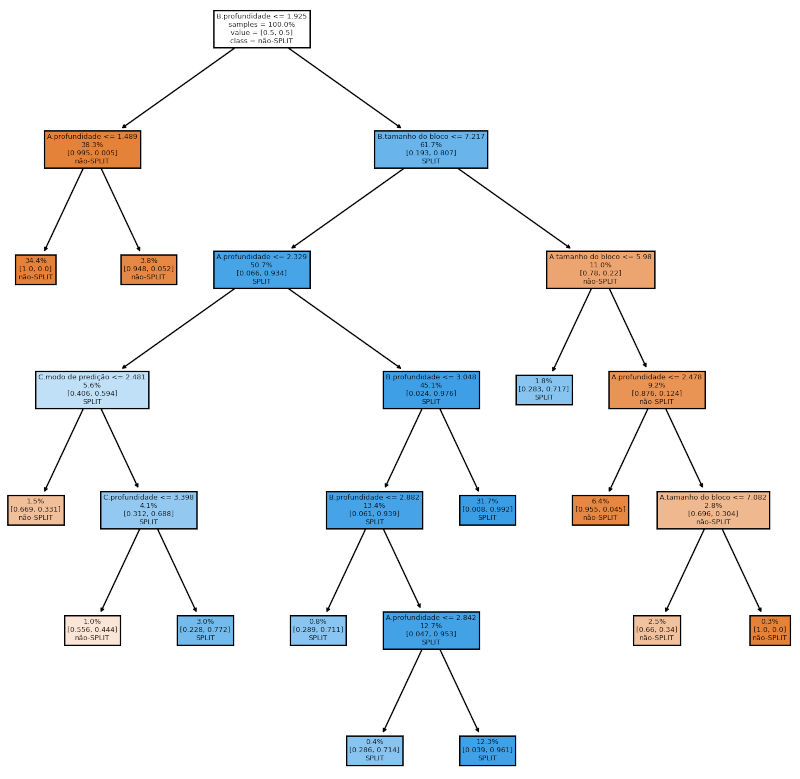
\includegraphics[width=\textwidth]{FIGURES/fig_34.png}
    \caption{Uma árvore de decisão gerada pelos modelos propostos. Fonte: Elaborada pelo autor.}
    \label{fig:34}
\end{figure}

Destes 12 modelos treinados com o conjunto completo de dados de treinamento, conforme explicitado na subseção \ref{cap:7.2.3}, e configurados conforme a Tabela \ref{tab:XXV}, foi possível obter os valores de F1-Score para todos os modelos e todas as propostas de transcodificador, conforme apresentados na Tabela \ref{tab:XXVI}. Nesta tabela, evidenciamos que a média obtida para a transcodificação de VP9 para AV1 é a maior de todas, apesar de que todas as demais apresentam valores muito próximos. Portanto, a expectativa é que os resultados de transcodificação sejam também próximos, principalmente relacionados ao impacto na eficiência da codificação. Analisando os resultados individuais de cada modelo presente na Tabela \ref{tab:XXVI}, é possível notar que o valor de \textit{F1-Score} decai conforme a profundidade aumenta. Por exemplo, o modelo do CQ 20 e profundidade 0 do transcodificador de H.266/VVC para AV1 possui um \textit{F1-Score} de 0,9929, enquanto que o modelo relacionado à profundidade 2 possui o valor de 0,9412. Apesar de ser uma diferença pequena, que se reflete em maior ou menor grau nos demais casos similares, hipotetiza-se que essa diferença implique em um erro de decisão maior nas sequências que requisitem uma profundidade maior da árvore de particionamento. Em outras palavras, vídeos que necessitem de maiores detalhes devem ter um impacto na eficiência de codificação maior que em sequências onde blocos grandes são mais utilizados, basicamente, em cenas mais paradas ou com grandes áreas homogêneas. 

\begin{table}
\begin{center}
\caption{Resultados da métrica \textit{F1-Score} obtidos com os modelos preditivos treinados sob os candidatos vencedores de cada proposta de transcodificação acelerado implementado.}
\label{tab:XXVI}
\footnotesize

\begin{tblr}{
    colspec = {l|r|r|r|r|r},
    hlines,
    row{even} = {gray9}
}
\hline
\textbf{Modelo do Conjunto} & \textbf{VP9} & \textbf{H.264/AVC} & \textbf{VP8} & \textbf{H.265/HEVC} & \textbf{H.266/VVC}\\
1 (CQ 20 P 0) & 0,9919 & 0,9917 & 0,9926 & 0,9928 & 0,9929\\
2 (CQ 20 P 1) & 0,9552 & 0,9796 & 0,9774 & 0,9551 & 0,9588\\
3 (CQ 20 P 2) & 0,9592 & 0,9362 & 0,9480 & 0,9480 & 0,9412\\
4 (CQ 32 P 0) & 0,9933 & 0,9928 & 0,9929 & 0,9933 & 0,9932\\
5 (CQ 32 P 1) & 0,9608 & 0,9560 & 0,9513 & 0,9554 & 0,9507\\
6 (CQ 32 P 2) & 0,9508 & 0,9535 & 0,9450 & 0,9520 & 0,9448\\
7 (CQ 43 P 0) & 0,9932 & 0,9931 & 0,9939 & 0,9930 & 0,9934\\
8 (CQ 43 P 1) & 0,9500 & 0,9447 & 0,9484 & 0,9520 & 0,9494\\
9 (CQ 43 P 2) & 0,9445 & 0,9418 & 0,9393 & 0,9419 & 0,9465\\
10 (CQ 55 P 0) & 0,9934 & 0,9935 & 0,9933 & 0,9934 & 0,9933\\
11(CQ 55 P 1) & 0,9591 & 0,9512 & 0,9552 & 0,9571 & 0,9465\\
12 (CQ 55 P 2) & 0,9330 & 0,9398 & 0,9344 & 0,9324 & 0,9389\\
\textbf{Média} & \textbf{0,9654} & \textbf{0,9645} & \textbf{0,9643} & \textbf{0,9639} & \textbf{0,9625}\\
\hline
\end{tblr}
\end{center}
\end{table}


Por fim, antes de apresentar os resultados obtidos, é preciso relembrar que a média de aceleração observada na literatura, conforme foi visto no capítulo \ref{cap:3}, é de 50,74\% de TS e de 4,11\% de BD-rate. Também ressaltamos neste capítulo que a comparação direta de qualquer solução com a média observada não pode ser feita de forma justa, haja visto a necessidade de se equiparar não apenas os formatos de transcodificação, como também as sequências utilizadas, as configurações aplicadas e a aplicabilidade alvo da proposta. Destacado essa injustiça ao se realizar qualquer comparação, nesta tese serão aplicadas comparações superficiais com a média, tendo em vista a ausência de melhores trabalhos para comparações. Ressalta-se, ainda, que mesmo propostas com valores com menor destaque ao observado na média da literatura não implicam diretamente em propostas ruins, pois, como já dissemos, quaisquer análises de resultados desconsideram contextos intrínsecos dos trabalhos desenvolvidos naquelas propostas, tampouco sobre os formatos de transcodificação utilizados. Dessa forma, apesar do uso de correlações com a média observada na literatura ter seu propósito de criar expectativas, essa análise não valida ou invalida quaisquer resultados.


\subsection{Transcodificação Rápida de VP9-para-AV1}
\label{cap:7.5.1}

A Tabela \ref{tab:XXVII} dispõe de todos os resultados obtidos para o transcodificador rápido de VP9 para AV1. Observa-se uma aceleração média da transcodificação de 16,76\%, a um custo de elevar o BD-rate em 5,10\%. Os três melhores resultados desta transcodificação estão na resolução HD1080, cuja resolução foi utilizado para realizar os treinamentos dos modelos preditivos. Nesta resolução em especial (HD1080), observa-se um TS de 19,58\% e um BD-rate de 4,47\%. As três sequências que apresentaram maior destaque são: \textit{crowd\_run\_1080p50\_60f}, \textit{ducks\_take\_off\_1080p50\_60f} e \textit{guitar\_hdr\_amazon\_1080p}, respectivamente com acelerações iguais a 36,81\%, 37,35\% e 51,96\%. Inclusive, a sequência \textit{guitar\_hdr\_amazon\_1080p} apresentou o maior TS entre todos os resultados de transcodificação rápida de VP9 para AV1. Apesar de serem sequências com cenas bem distintas (como pode ser visto no Apêndice \ref{apx:A}), indo desde patos nadando em um lago até um grupo de pessoas correndo montanha abaixo, há algo que é similar entre eles: são cenas de movimento em toda a área do quadro. Isso indica que as sequências devam usar uma quantidade maior de blocos menores, sugerindo que os modelos preditivos, pelo menos para as profundidades 0 e 1, são eficientes em predizer corretamente o particionamento do bloco.

\begin{center}
{\footnotesize
\begin{longtblr}[
    caption = {Resultados da transcodificação rápida de VP9 para AV1 baseado em modelos preditivos.},
    label = {tab:XXVII}
]{
    colspec = {l|p{6cm}|r|r|r},
    hlines,
    row{even} = {gray9}
}
\hline
\textbf{Resolução} & \textbf{Sequência} & \textbf{BD-rate (\%)} & \textbf{TS (\%)} & \textbf{Razão}\\
\SetCell[r=12]{l}HD720 & boat\_hdr\_amazon\_720p & 4,2537 & 13,99 & 0,304\\
 & dark720p\_120f & 5,4006 & 19,44 & 0,278\\
 & FourPeople\_1280x720\_60 & 2,4022 & 7,98 & 0,301\\
 & FourPeople\_1280x720\_60\_120f & 2,3122 & 8,05 & 0,287\\
 & gipsrestat720p\_120f & 2,6988 & 11,76 & 0,229\\
 & Johnny\_1280x720\_60 & 4,0714 & 14,33 & 0,284\\
 & Johnny\_1280x720\_60\_120f & 3,8174 & 15,76 & 0,242\\
 & KristenAndSara\_1280x720\_60 & 3,0265 & 16,69 & 0,181\\
 & KristenAndSara\_1280x720\_60\_120f & 3,0265 & 16,63 & 0,182\\
 & Netflix\_DinnerScene\_1280x720\_60fps \_8bit\_420\_120f & 6,3817 & 27,47 & 0,232\\
 & Netflix\_DrivingPOV\_1280x720\_60fps \_8bit\_420\_120f & 3,0173 & 12,54 & 0,241\\
 & Netflix\_FoodMarket2\_1280x720\_60fps \_8bit\_420\_120f & 2,966 & 8,99 & 0,330\\
\SetCell[r=8]{l}HD720 & Netflix\_RollerCoaster\_1280x720\_60fps \_8bit\_420\_120f & 5,7515 & 25,11 & 0,229\\
 & Netflix\_Tango\_1280x720\_60fps\_8bit \_420\_120f & 4,3562 & 8,07 & 0,540\\
 & rain\_hdr\_amazon\_720p & 1,0663 & 7,37 & 0,145\\
 & vidyo1\_720p\_60fps\_120f & 3,2613 & 12,9 & 0,253\\
 & Vidyo3\_1280x720\_60 & 3,8858 & 14,11 & 0,275\\
 & vidyo3\_720p\_60fps\_120f & 3,6996 & 14,16 & 0,261\\
 & Vidyo4\_1280x720\_60 & 2,9377 & 13,09 & 0,225\\
 & vidyo4\_720p\_60fps\_120f & 3,1043 & 12,99 & 0,239\\
\SetCell[c=2]{r}\textbf{Média dos vídeos HD720} && \textbf{3,5718} & \textbf{14,07} & \\
\SetCell[r=17]{l}HD1080 & aspen\_1080p\_60f & 5,7618 & 9,11 & 0,632\\
 & crowd\_run\_1080p50\_60f & 2,736 & 36,81 & 0,074\\
 & ducks\_take\_off\_1080p50\_60f & 4,4386 & 37,35 & 0,119\\
 & guitar\_hdr\_amazon\_1080p & 6,3438 & 51,96 & 0,122\\
 & Netflix\_Aerial\_1920x1080\_60fps\_8bit \_420\_60f & 4,2699 & 29,04 & 0,147\\
 & Netflix\_Boat\_1920x1080\_60fps\_8bit \_420\_60f & 1,7737 & 18,42 & 0,096\\
 & Netflix\_Crosswalk\_1920x1080\_60fps \_8bit\_420\_60f & 3,7432 & 24,88 & 0,150\\
 & Netflix\_FoodMarket\_1920x1080\_60fps \_8bit\_420\_60f & 4,862 & 12,47 & 0,390\\
 & Netflix\_PierSeaside\_1920x1080\_60fps \_8bit\_420\_60f & 3,9322 & 9,41 & 0,418\\
 & Netflix\_SquareAndTimelapse\_1920x 1080\_60fps\_8bit\_420\_60f & 3,7862 & 8,64 & 0,438\\
 & Netflix\_TunnelFlag\_1920x1080\_60fps \_8bit\_420\_60f & 7,6284 & 28,33 & 0,269\\
 & old\_town\_cross\_1080p50\_60f & 7,6534 & 16,34 & 0,468\\
 & park\_joy\_1080p50\_60f & 2,012 & 9,3 & 0,216\\
 & pedestrian\_area\_1080p25\_60f & 4,2314 & 9,42 & 0,449\\
 & rush\_field\_cuts\_1080p\_60f & 2,4349 & 14,08 & 0,173\\
 & rush\_hour\_1080p25\_60f & 4,5744 & 11,41 & 0,401\\
 & seaplane\_hdr\_amazon\_1080p & 3,1675 & 14,68 & 0,216\\
HD1080 & station2\_1080p25\_60f & 7,2066 & 10,69 & 0,674\\
\SetCell[c=2]{r}\textbf{Média dos vídeos HD1080} && \textbf{4,4753} & \textbf{19,58} & \\
\SetCell[r=6]{l}UHD4K & Netflix\_BoxingPractice\_4096x2160 \_60fps\_10bit\_420\_60f & 11,0334 & 18,01 & 0,613\\
 & Netflix\_Dancers\_4096x2160\_60fps \_10bit\_420\_60f & 24,0996 & 17,77 & 1,356\\
 & Netflix\_Narrator\_4096x2160\_60fps \_10bit\_420\_60f & 12,2722 & 22,98 & 0,534 \\
 & Netflix\_RitualDance\_4096x2160\_60fps \_10bit\_420\_60f & 14,1521 & 20,86 & 0,679 &  & \\
 & Netflix\_ToddlerFountain\_4096x2160 \_60fps\_10bit\_420\_60f & 2.8256 & 19,93 & 0,142 \\
 & Netflix\_WindAndNature\_4096x2160 \_60fps\_10bit\_420\_60f & 8,0698 & 3,96 & 2,038
 \\
\SetCell[c=2]{r}\textbf{Média dos vídeos UHD4K} && \textbf{12,0755} & \textbf{17,25}  & \\
\SetCell[c=2]{r}\textbf{Média Geral} && \textbf{5,1010} & \textbf{16,76} & \\
\SetCell[c=2]{r}\textbf{Desvio Padrão Geral} && \textbf{3,9862} & \textbf{9,30} & \\
\hline
\end{longtblr}
}
\end{center}



Se os resultados observados na resolução HD1080 apresentam resultados positivos em algumas condições, adaptar a proposta para uma resolução menor, como HD720, não trouxe impactos negativos. Inclusive, apresenta resultados similares de redução do tempo (média de 14,07\%) e de impacto na eficiência de codificação (média de 3,57\%) em relação aos resultados observados na resolução HD1080. Nesta resolução, a sequência com a menor Razão foi \textit{rain\_hdr\_amazon\_720p}, com 0,145 pontos, originários de uma aceleração de 7,37\% da transcodificação e um BD-rate de 1,06\%. A sequência HD720 que obteve o maior TS foi \textit{Netflix\_DinnerScene\_1280x720\_60fps\_8bit\_420\_120f} com 27,47\%, mas o BD-rate foi de 6,38\%. Coincidentemente, é com esta sequência de vídeo que se observa o maior BD-rate para a resolução HD720. Todavia, quase todos os vídeos UHD4K não apresentaram resultados satisfatórios de eficiência de codificação, com resultados de BD-rate superiores a 8\% e uma aceleração inferior à 22,98\% (vista na sequência \textit{Netflix\_Narrator\_4096x2160\_60fps\_10bit\_420\_60f}). A única exceção é \textit{Netflix\_ToddlerFountain\_4096x2160\_60fps\_10bit\_420\_60f}, que apresenta 2,82\% de BD-rate e 19,93\% de TS. 

Há, publicado na literatura científica, outra proposta de transcodificador rápido de VP9 para AV1, que desenvolvemos e apresentamos na seção \ref{cap:6.2}. Essa proposta apresentou uma redução de complexidade de 28,16\% a um custo na eficiência de codificação de 4,34\%. Essa proposta de transcodificador rápido não utiliza modelos preditivos para auxiliar nas decisões rápidas e, portanto, consegue apresentar uma média geral melhor que a proposta apresentada nesta subseção, baseada em modelos preditivos. Contudo, o trabalho descrito na seção \ref{cap:6.2} utiliza um conjunto menor de vídeos para avaliar os resultados, apesar de apresentar uma maior variedade de resoluções. Se considerarmos apenas as mesmas sequências utilizadas nas duas propostas, obteremos os dados apresentados na Tabela \ref{tab:XXVIII}, onde comparamos diretamente as duas propostas apresentadas nesta tese para a transcodificação rápida de VP9 para AV1.

\begin{table}
\begin{center}
\caption{Relação direta entre as propostas de transcodificador rápido do formato VP9 para o AV1.}
\label{tab:XXVIII}
\footnotesize

\begin{tblr}{
    colspec = {p{4cm}|r|r|r|r|r|r},
    hlines,
    row{even} = {gray9}
}
\hline
& \SetCell[c=3]{c}\textbf{Proposta com Modelos Preditivos} &&& \SetCell[c=3]{c}\textbf{Proposta com Heurística} &&\\
\textbf{Sequência} & \textbf{BD-rate (\%)} & \textbf{TS (\%)} & \textbf{Razão} & \textbf{BD-rate (\%)} & \textbf{TS (\%)} & \textbf{Razão} \\
dark720p\_120f & 5,40 & 19,44 & 0,28 & 4,14 & 23,02 & 0,18 \\
Johnny\_1280x720\_60\_ 120f & 3,82 & 15,76 & 0,24 & 6,05 & 24,74 & 0,24 \\
Netflix\_DrivingPOV\_1280x 720\_60fps\_8bit\_420\_120f & 3,02 & 12,54 & 0,24 & 6,37 & 31,58 & 0,20 \\
Netflix\_RollerCoaster\_ 1280x720\_60fps\_8bit\_420\_120f & 5,75 & 25,11 & 0,23 & 6,69 & 41,73 & 0,16 \\
\SetCell[c=1]{r}\textbf{Média da resolução HD720} & \textbf{4,50} & \textbf{18,21} & \textbf{0,25} & \textbf{5,81} & \textbf{30,27} & \textbf{0,19} \\
crowd\_run\_1080p50\_60f & 2,74 & 36,81 & 0,07 & 3,53 & 34,25 & 0,10 \\
Netflix\_Crosswalk\_1920x 1080\_60fps\_8bit\_420\_60f & 3,74 & 24,88 & 0,15 & 4,00 & 18,01 & 0,22 \\
park\_joy\_1080p50\_60f & 2,01 & 9,30 & 0,22 & 5,86 & 42,67 & 0,14 \\
seaplane\_hdr\_amazon\_ 1080p & 3,17 & 14,68 & 0,22 & 4,98 & 24,53 & 0,20 \\
\SetCell[c=1]{r}\textbf{Média da resolução HD1080} & \textbf{2,91} & \textbf{21,42} & \textbf{0,14} & \textbf{4,60} & \textbf{29,87} & \textbf{0,15} \\
\SetCell[c=1]{r}\textbf{Média Geral} & \textbf{3,71} & \textbf{19,81} & \textbf{0,19} & \textbf{5,20} & \textbf{30,07} & \textbf{0,17}\\
\hline
\end{tblr}
\end{center}
\end{table}


Na Tabela \ref{tab:XXVIII} podemos observar que o impacto na eficiência de codificação gerado pela proposta baseada em modelos preditivos é menor que o da proposta baseada em heurística. Isso significa que os modelos treinados geram decisões mais assertivas, principalmente na resolução HD1080 (2,91\% contra os 4,60\%). Observe que as sequências \textit{crowd\_run\_1080p50\_60f} e \textit{Netflix\_Crosswalk\_1920x1080\_60fps\_8bit\_420\_60f} apresentaram resultados melhores, tanto em BD-rate como em TS, ao utilizar a proposta baseada em modelos preditivos. Todavia, a aceleração geral obtida com as propostas usando modelos preditivos é menor, em especial para a sequência \textit{park\_joy\_1080p50\_60f}, que foi acelerada em 42,67\% na proposta da seção 6.2 contra os 9,30\% da proposta deste capítulo.

Desta forma, foi preciso investigar a causa do valor de TS inferior. Identificou-se que o algoritmo de transcodificação rápida proposto, em especial na manipulação das matrizes citadas na subseção \ref{cap:7.4.1}, consomem um tempo de processamento significativamente elevado no transcodificador. Avaliando a sequência de vídeo \textit{crowd\_run\_1080p50\_60f} sob o nível de quantização 20, na transcodificação original esta tarefa foi executada em 60.466 segundos (ou 16,8 horas), enquanto que na transcodificação rápida a mesma sequência de vídeo foi processada em 42.181 segundos (11,7 horas). Apesar de podermos perceber uma redução do custo computacional em 30\% nesta única sequência, observaram-se 2.974 segundos (49,6 minutos) do tempo do transcodificador dedicados ao algoritmo desenvolvido, isto é, 7,05\%. O mesmo se observou em outra sequência de vídeo (\textit{pan\_hdr\_amazon\_1080p}) sob um nível de quantização diferente (CQ 43), que codificou em 24.484 segundos na transcodificação original contra os 19.424 segundos na transcodificação rápida, ou seja, atingiu uma redução de 20\% do tempo. No entanto, foram necessários 1.344 segundos na execução do algoritmo, ou seja, 6.92\% do tempo total da codificação do \textit{libaom}. Casos similares puderam ser vistos em outras sequências sob níveis de quantização diferentes, com consumos de tempo próximos a 7\%.

Portanto, conclui-se que é possível obter resultados melhores de redução de tempo, caso o algoritmo desenvolvido seja otimizado, a um teto de 7\%, caso sua execução atinja o tempo real. Assim sendo, dos resultados médios de aceleração da resolução HD1080, apresentados na Tabela \ref{tab:XXVII} (de 19,58\%), seria possível estimar um resultado de TS máximo de 26,57\%.

\subsection{Transcodificação Rápida de H.264/AVC-para-AV1}
\label{cap:7.5.2}

A proposta de transcodificador rápido desenvolvida de VP9 para AV1 foi adaptada de H.264/AVC para AV1, utilizando o \textit{pipeline} de processamento. Utilizando as mesmas sequências de vídeo descritas anteriormente, exceto para vídeos UHD4K, foi possível obter uma aceleração da transcodificação de 25,05\% a um custo de reduzir a eficiência de codificação em 5,58\%, como é possível notar na Tabela \ref{tab:XXIX}. Uma observação geral que pode ser vista nesta proposta de transcodificador, em relação ao caso VP9 para AV1, é que os resultados foram melhores para a resolução HD720, ao invés da resolução HD1080. O TS médio obtido na resolução HD720 foi de 30,52\%, contra os 18,67\% da resolução HD1080. Inclusive, o impacto na eficiência de codificação também é menor na resolução HD720 (5,30\% contra 5,91\%). Como o formato H.264/AVC foi desenvolvido para lidar principalmente com resoluções HD720 ou inferiores, supõe-se que as demais informações dos atributos, além das médias de profundidades e de tamanho de bloco, possam contribuir mais para a tomada de decisão nessas resoluções, mesmo utilizando um modelo preditivo treinado para uma resolução maior.

\begin{center}
{\footnotesize
\begin{longtblr}[
 caption = {Resultados da transcodificação rápida de H.264/AVC para AV1 baseada em modelos preditivos.},
 label = {tab:XXIX}
]{
 colspec = {l|p{6cm}|r|r|r},
 hlines,
 row{even} = {gray9}
}
\hline
\textbf{Resolução} & \textbf{Sequência} & \textbf{BD-rate (\%)} & \textbf{TS (\%)} & \textbf{Razão}\\
\SetCell[r=21]{c}HD720 & boat\_hdr\_amazon\_720p & 0,7029 & 12,91 & 0,054 \\
 & dark720p\_120f & 9,1593 & 42,26 & 0,217 \\
 & FourPeople\_1280x720\_60 & 2,6325 & 32,32 & 0,081 \\
 & FourPeople\_1280x720\_60\_120f & 2,5755 & 32,47 & 0,079 \\
 & gipsrestat720p\_120f & 3,6448 & 40,85 & 0,089 \\
 & Johnny\_1280x720\_60 & 7,7357 & 48,34 & 0,160 \\
 & Johnny\_1280x720\_60\_120f & 8,0233 & 49,13 & 0,163 \\
 & KristenAndSara\_1280x720\_60 & 6,0619 & 47,96 & 0,126 \\
 & KristenAndSara\_1280x720\_60\_120f & 6,0619 & 47,97 & 0,126 \\
 & Netflix\_DinnerScene\_1280x720\_60fps \_8bit\_420\_120f & 13,0913 & 37,94 & 0,345 \\
 & Netflix\_DrivingPOV\_1280x720\_60fps \_8bit\_420\_120f & 4,3667 & 17,2 & 0,254 \\
 & Netflix\_FoodMarket2\_1280x720\_60fps \_8bit\_420\_120f & 4,0778 & 20,33 & 0,201 \\
 & Netflix\_RollerCoaster\_1280x720\_60fps \_8bit\_420\_120f & 6,7889 & 43,18 & 0,157 \\
 & Netflix\_Tango\_1280x720\_60fps\_8bit \_420\_120f & 4,3732 & 9,2 & 0,475 \\
 & rain\_hdr\_amazon\_720p & 0,5833 & 10,98 & 0,053 \\
 & Vidyo1\_1280x720\_60 & 4,1503 & 16,69 & 0,249 \\
 & vidyo1\_720p\_60fps\_120f & 3,9878 & 17,05 & 0,234 \\
 & Vidyo3\_1280x720\_60 & 2,8683 & 8,04 & 0,357 \\
 & vidyo3\_720p\_60fps\_120f & 2,3452 & 8,75 & 0,268 \\
 & Vidyo4\_1280x720\_60 & 9,1446 & 48,11 & 0,190 \\
 & vidyo4\_720p\_60fps\_120f & 8,9525 & 49,16 & 0,182 \\
\SetCell[c=2]{r}\textbf{Média dos vídeos HD720} && \textbf{5,3013} & \textbf{30,52} & \\
\SetCell[r=5]{c}HD1080 & aspen\_1080p\_60f & 15,1526 & 33,99 & 0,446 \\
 & crowd\_run\_1080p50\_60f & 0,8863 & 15,65 & 0,057 \\
 & ducks\_take\_off\_1080p50\_60f & 3,3596 & 25,83 & 0,130 \\
 & guitar\_hdr\_amazon\_1080p & 1,1848 & 12,73 & 0,095 \\
 & Netflix\_Aerial\_1920x1080\_60fps\_8bit \_420\_60f & 5,1584 & 20,96 & 0,246 \\
\SetCell[r=13]{c}HD1080 & Netflix\_Boat\_1920x1080\_60fps\_8bit \_420\_60f & 1,8815 & 20,37 & 0,092 \\
 & Netflix\_Crosswalk\_1920x1080\_60fps \_8bit\_420\_60f & 10,3418 & 12,52 & 0,826 \\
 & Netflix\_FoodMarket\_1920x1080\_60fps \_8bit\_420\_60f & 9,5122 & 19,58 & 0,486 \\
 & Netflix\_PierSeaside\_1920x1080\_60fps \_8bit\_420\_60f & 11,0504 & 41,32 & 0,267 \\
 & Netflix\_SquareAndTimelapse\_1920x 1080\_60fps\_8bit\_420\_60f & 3,0506 & 12,59 & 0,240 \\
 & Netflix\_TunnelFlag\_1920x1080\_60fps \_8bit\_420\_60f & 6,7701 & 17,9 & 0,380 \\
 & old\_town\_cross\_1080p50\_60f & 6,3312 & 21,54 & 0,294 \\
 & park\_joy\_1080p50\_60f & 1,0161 & 12,37 & 0,082 \\
 & pedestrian\_area\_1080p25\_60f & 8,176 & 14,23 & 0,575 \\
 & rush\_field\_cuts\_1080p\_60f & 1,0555 & 13,72 & 0,077 \\
 & rush\_hour\_1080p25\_60f & 8,4783 & 14,01 & 0,605 \\
 & seaplane\_hdr\_amazon\_1080p & 0,324 & 5,71 & 0,057 \\
 & station2\_1080p25\_60f & 12,7702 & 21,11 & 0,605 \\
\SetCell[c=2]{r}\textbf{Média dos vídeos HD1080} && \textbf{5,9166} & \textbf{18,67} & \\
\SetCell[c=2]{r}\textbf{Média Geral} && \textbf{5,5853} & \textbf{25,05} & \\
\SetCell[c=2]{r}\textbf{Desvio Padrão Geral} && \textbf{3,8649} & \textbf{14,28} & \\
\hline
\end{longtblr}
}
\end{center}



Os principais destaques na transcodificação de H.264/AVC para AV1 são para as sequências \textit{boat\_hdr\_amazon\_720p}, \textit{rain\_hdr\_amazon\_720p}, \textit{crowd\_run\_1080p50\_60f} e \textit{seaplane\_hdr\_amazon\_1080p}, todos com menos de 0,06 pontos de Razão. Uma característica entre essas sequências é que há uma metade da cena relativamente estática e outra com muitos movimentos, geralmente de água ou de pessoas distantes. Isso significa que há uma mescla homogênea entre tamanhos de bloco, o que, somado às demais informações extraídas dos atributos do H.264/AVC em relação ao VP9, pode impulsionar uma melhora significativa dos resultados observados nesta proposta de transcodificador rápido.

No entanto, há sete sequências HD1080 na Tabela \ref{tab:XXIX} que podem ser enquadradas como resultados negativos, sendo que quatro delas ultrapassam a marca de 10\% de BD-rate. Em especial \textit{Netflix\_Crosswalk\_1920x1080\_60fps\_8bit\_420\_60f}, que apresenta a maior Razão entre todas as sequências, com 12,52\% de TS e 10,34\% de BD-rate. Nota-se uma inversão completa em relação à proposta de VP9 para AV1, onde esta mesma sequência foi uma das de maior destaque, apresentando 24,88\% de TS e 3,74\% de BD-rate. Não identificamos uma causa para essa inversão específica.

Como visto na Tabela \ref{tab:III}, não há outros trabalhos de transcodificação de H.264/AVC para AV1. Portanto, esta é uma proposta inédita de transcodificador rápido e não existem comparações diretas que possam ser feitas. Todavia, observa-se uma média de aceleração dos trabalhos apresentados na literatura científica com o dobro do percentual apresentado do transcodificador apresentado neste subseção. Apesar de não ser possível fazer uma comparação justa dos resultados deste transcodificador rápido com a média da literatura, como já abordamos no Capítulo \ref{cap:3}, ainda assim a redução média de um quarto do tempo do transcodificador rápido, em relação ao transcodificador original, é um resultado positivo.

Considerando os valores de razão próximos ao apresentado pela proposta desenvolvida nesta subseção (de 0,13), os nossos resultados podem ser comparados diretamente com os valores obtidos por \citet{bib:peixoto_2012} (52,75\% de TS e 5,49\% de BD-rate), \citet{bib:peixoto2_2014} (74,54\% de TS e 8,41\% de BD-rate) e \citet{bib:franche_2017} (87,32\% de TS e 3,28\% de BD-rate). Destes trabalhos, \citet{bib:franche_2017} também utiliza informações provenientes tanto do decodificador como do codificador, apesar de sua proposta ser baseada em heurísticas. Por outro lado, \citet{bib:peixoto2_2014} propõe uma solução baseada em modelos preditivos gerados por \textit{Linear Discriminant Function} \cite{bib:shumway_1974}.

\subsection{Transcodificação Rápida de VP8-para-AV1}
\label{cap:7.5.3}

O formato de codificação de vídeo VP8 é o antecessor do formato VP9 e, como visto anteriormente nesta tese, possui uma série de limitações em comparação aos formatos mais recentes. Por exemplo, o VP8 só permite dois tamanhos de blocos, cada um voltado para um tipo de predição específico: interquadros (blocos de 16$\times$16) e intraquadro (blocos de 4$\times$4). Além disso, o formato não tem a capacidade de trabalhar com vídeos HDR e nem com subamostragem diferente de 4:2:0. Tais limitações e diferenças significativas do  formato VP8, explicam, em parte, os resultados obtidos na Tabela \ref{tab:XXXI}. Nesta tabela, observamos que a proposta de transcodificador rápido de VP8 para AV1, baseado em modelos preditivos, atinge uma aceleração de 55,69\% em relação ao transcodificador original, a melhor média de TS dentre todas as propostas desta tese e similar ao observado na literatura. No entanto, a solução impacta a eficiência de codificação em 12,85\% de BD-rate e, mesmo assim, ainda é uma solução inédita na literatura.

\begin{center}
{\footnotesize
\begin{longtblr}[
    caption = {Resultados obtidos com a transcodificação acelerada de VP8-para-AV1.},
    label = {tab:XXXI}
]{
    colspec = {l|p{6cm}|r|r|r},
    hlines,
    row{even} = {gray9},
    cell{10}{1} = {white},
    cell{34}{1} = {white}
}
\hline
\textbf{Resolução} & \textbf{Sequência} & \textbf{BD-rate (\%)} & \textbf{TS (\%)} & \textbf{Razão}\\
\SetCell[r=19]{c}HD720 & dark720p\_120f & 23,1199 & 76,25 & 0,303\\
 & FourPeople\_1280x720\_60 & 6,4063 & 71,03 & 0,090\\
 & FourPeople\_1280x720\_60\_120f & 6,5943 & 70,76 & 0,093\\
 & gipsrestat720p\_120f & 10,7597 & 77,57 & 0,139\\
 & Johnny\_1280x720\_60 & 16,2512 & 79,12 & 0,205\\
 & Johnny\_1280x720\_60\_120f & 16,2456 & 79,7 & 0,204\\
 & KristenAndSara\_1280x720\_60 & 13,4166 & 80,78 & 0,166\\
 & KristenAndSara\_1280x720\_60\_120f & 13,4166 & 80,87 & 0,166\\
 & Netflix\_DinnerScene\_1280x720\_60fps \_8bit\_420\_120f & 25,6688 & 62,58 & 0,410\\
 & Netflix\_DrivingPOV\_1280x720\_60fps \_8bit\_420\_120f & 10,9251 & 64,91 & 0,168\\
 & Netflix\_FoodMarket2\_1280x720\_60fps \_8bit\_420\_120f & 8,0288 & 34,59 & 0,232\\
 & Netflix\_RollerCoaster\_1280x720\_60fps \_8bit\_420\_120f & 15,327 & 66,61 & 0,230\\
 & Netflix\_Tango\_1280x720\_60fps\_8bit \_420\_120f & 7,5238 & 21,39 & 0,352\\
 & Vidyo1\_1280x720\_60 & 6,563 & 23,72 & 0,277\\
 & vidyo1\_720p\_60fps\_120f & 6,3635 & 24,61 & 0,259\\
 & Vidyo3\_1280x720\_60 & 11,6042 & 73,5 & 0,158\\
 & vidyo3\_720p\_60fps\_120f & 10,8592 & 73,31 & 0,148\\
 & Vidyo4\_1280x720\_60 & 16,2467 & 76,42 & 0,213\\
 & vidyo4\_720p\_60fps\_120f & 16,0305 & 76,03 & 0,211\\
\SetCell[c=2]{r}\textbf{Média dos vídeos HD720} && \textbf{12,7027} & \textbf{63,88} & \\
\SetCell[r=6]{c}HD1080 & aspen\_1080p\_60f & 24,1958 & 29,86 & 0,810\\
 & crowd\_run\_1080p50\_60f & 1,5514 & 30,57 & 0,051\\
 & ducks\_take\_off\_1080p50\_60f & 4,4886 & 49,62 & 0,090\\
 & Netflix\_Aerial\_1920x1080\_60fps\_8bit \_420\_60f & 10,7455 & 37,82 & 0,284\\
 & Netflix\_Boat\_1920x1080\_60fps\_8bit \_420\_60f & 2,8285 & 31,87 & 0,089\\
 & Netflix\_Crosswalk\_1920x1080\_60fps \_8bit\_420\_60f & 23,1568 & 32,74 & 0,707\\
\SetCell[r=10]{c}HD1080 & Netflix\_FoodMarket\_1920x1080\_60fps \_8bit\_420\_60f & 16,0831 & 32,88 & 0,489\\
 & Netflix\_PierSeaside\_1920x1080\_60fps \_8bit\_420\_60f & 14,2656 & 76,93 & 0,185\\
 & Netflix\_SquareAndTimelapse\_1920x 1080\_60fps\_8bit\_420\_60f & 4,9242 & 26,52 & 0,186\\
 & Netflix\_TunnelFlag\_1920x1080\_60fps \_8bit\_420\_60f & 11,5801 & 33,64 & 0,344\\
 & old\_town\_cross\_1080p50\_60f & 20,4893 & 76,59 & 0,268\\
 & park\_joy\_1080p50\_60f & 2,2236 & 54,74 & 0,041\\
 & pedestrian\_area\_1080p25\_60f & 22,9798 & 72,67 & 0,316\\
 & rush\_field\_cuts\_1080p\_60f & 1,9172 & 30,92 & 0,062\\
 & rush\_hour\_1080p25\_60f & 22,3852 & 75,96 & 0,295\\
 & station2\_1080p25\_60f & 24,689 & 42,05 & 0,587\\
\SetCell[c=2]{r}\textbf{Média dos vídeos HD1080} && \textbf{13,0315} & \textbf{45,96} & \\
\SetCell[c=2]{r}\textbf{Média Geral} && \textbf{12,853} & \textbf{55,69} & \\
\SetCell[c=2]{r}\textbf{Desvio Padrão Geral} && \textbf{7,2509} & \textbf{21,75} & \\
\hline
\end{longtblr}
}
\end{center}



Embora os resultados médios não sejam positivos em termos de eficiência de codificação, principalmente quando comparamos com a média da literatura, alguns destaques podem ser feitos, principalmente quanto à resolução HD1080. As três sequências de menor BD-rate são \textit{crowd\_run\_1080p50\_60f}, \textit{rush\_field\_cuts\_1080p\_60f} e \textit{park\_joy\_1080p50\_60f}, com respectivamente 1,55\%, 1,91\% e 2,22\% de BD-rate e com reduções de complexidade de 30,57\% 30,92\% e 54,74\%. Não encontrou-se uma similaridade direta entre essas três sequências. No entanto, após uma investigação avaliando outras características dos vídeos, percebeu-se que todos são vídeos com uma grande taxa de informação espacial (do inglês, \textit{Spatial Information}, SI). Conforme podemos ver na descrição das sequências no Apêndice \ref{apx:A}, as seis sequências HD1080 com mais de 60 pontos de SI são, em ordem crescente: \textit{ducks\_take\_off\_1080p50\_60f}, \textit{rush\_field\_cuts\_1080p\_60f}, \textit{Netflix\_Boat\_1920x1080\_60fps\_8bit\_420\_60f}, \textit{Netflix\_TunnelFlag\_1920x1080\_60fps\_8bit\_420\_60f}, \textit{park\_joy\_1080p50\_60f} e \textit{crowd\_run\_1080p50\_60f}. Destas, apenas a sequência \textit{Netflix\_TunnelFlag\_1920x1080\_60fps\_8bit\_420\_60f} apresenta resultados ruins para a solução proposta.

A sequência com a maior Razão é \textit{aspen\_1080p\_60f}. Observando os resultados de codificação dessa sequência, notamos uma perda de PSNR de -1,067dB no nível de quantização 55. Essa perda de qualidade somada ao aumento de 41,6\% da taxa de bits de \textit{aspen\_1080p\_60f} nesse nível de quantização, justificam o BD-rate de 24,19\%. Para exemplificar essa diferença de PSNR, apresentamos na Figura \ref{fig:35} uma parte de maior destaque do último quadro da sequência \textit{aspen\_1080p\_60f}. sob o nível de quantização 55. Os quadros apresentados na Figura \ref{fig:35} estão em diferentes momentos: Figura \ref{fig:35}(a) apresenta o quadro original, sem compressão seguido pela sua aparência após a decodificação do VP8 (Figura \ref{fig:35}(b)). Na Figura \ref{fig:35}(c) apresenta o quadro codificado pelo transcodificador original e Figura \ref{fig:35}(d) apresenta o quadro codificado pelo transcodificador rápido. Como é possível observar nestas figuras, nota-se uma perda da nitidez das folhas, em especial do interior delas. Apesar das ranhuras e das manchas da folha se perderem um pouco após a codificação por parte do VP8, ainda é possível percebê-las após a decodificação (Figura \ref{fig:35}(b)). Todavia, após a transcodificação para o AV1, quase todas as ranhuras se perdem, em especial quando transcodificadas pela nossa proposta rápida, restando na cena um borrão verde. E apesar da sequência \textit{aspen\_1080p\_60f}, assim como a maioria das sequências com BD-rate acima dos 20\%, também serem sequências com valores negativos na transcodificação de H.264/AVC para AV1, não foi possível identificar alguma característica intrínseca ao vídeo que auxiliasse na explicação desses valores elevados de BD-rate.

\begin{figure}
    \centering
    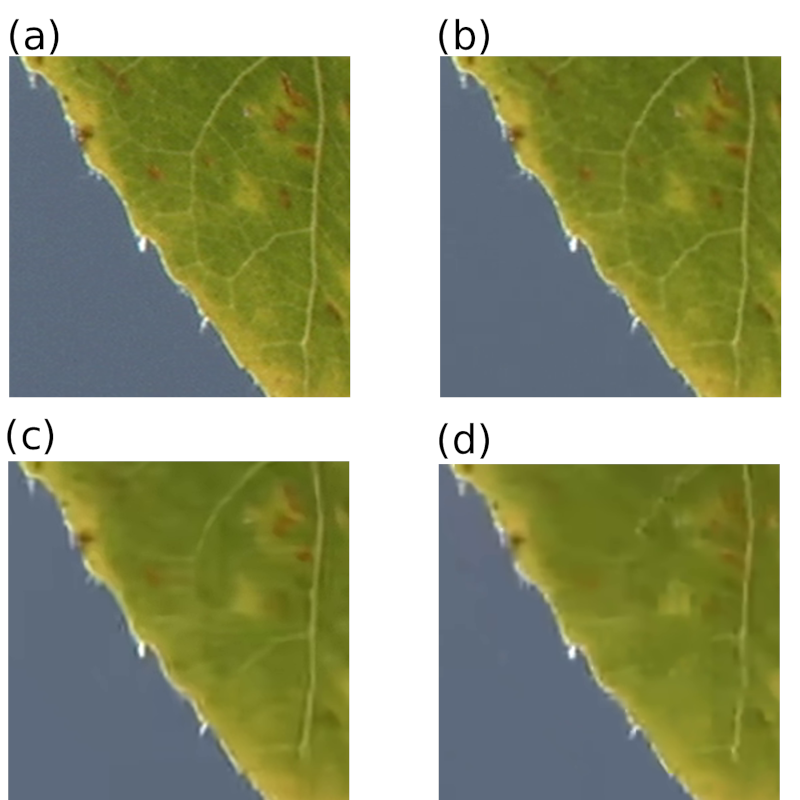
\includegraphics[width=\textwidth]{FIGURES/fig_35.png}
    \caption{Destaque do último quadro do vídeo \textit{aspen\_1080p\_60f} para as sequências (a) original, (b) decodificada pelo VP8, (c) transcodificada original para o AV1 e (d) transcodificada acelerada para o AV1. Fonte: Elaborada pelo autor.}
    \label{fig:35}
\end{figure}


\subsection{Transcodificação Rápida de H.265/HEVC-para-AV1}
\label{cap:7.5.4}

A Tabela \ref{tab:XXXIII} apresenta os resultados obtidos com a transcodificação rápida de H.265/HEVC para AV1, cujo algoritmo foi desenvolvido seguindo a mesma metodologia da proposta de VP9 para AV1. Nesta tabela, é possível observar que a solução é capaz de atingir uma aceleração da transcodificação de 28,36\%, a um custo de 6,74\% de BD-rate. A sequência de maior destaque é \textit{ducks\_take\_off\_1080p50\_60f}, com 41,64\% de TS e 4,10\% de BD-rate. Assim como os resultados de H.264/AVC e de VP8, na proposta para o H.265/HEVC observa-se uma maior redução de tempo nas sequências HD720 do que nas sequências HD1080, para os quais os modelos foram treinados. O fato de só haver uma única sequência HD720 que é caso destacadamente negativa (\textit{dark720p\_120f}), contra os cinco exemplos da resolução HD1080 (\textit{Netflix\_Aerial\_1920x1080\_60fps\_8bit\_420\_60f}, \textit{Netflix\_Crosswalk\_1920x1080\_60fps\_8bit\_420\_60f}, \textit{Netflix\_FoodMarket\_1920x1080\_60fps\_8bit\_420\_60f}, \textit{pedestrian\_area\_1080p25\_60f} e \textit{station2\_1080p25\_60f}) conta bastante para essa diferença em favor da resolução menor, mesmo que pequena. Outro ponto de destaque na proposta de H.265/HEVC para AV1 é que, diferentemente do que observamos no transcodificador rápido de VP9 para AV1, os resultados obtidos na transcodificação de vídeos UHD4K não são compostos por casos negativos. Apesar da baixa aceleração obtida, todos possuem valores de BD-rate baixos (menos de 3,2\%). Isso indica que as amostras geradas pelo decodificador H.265/HEVC em vídeos UHD4K fornecem dados mais confiáveis e de maior qualidade que os gerados pelo decodificador VP9.

\begin{center}
{\footnotesize
\begin{longtblr}[
    caption = {Resultados da transcodificação rápida de H.265/HEVC para AV1 baseado em modelos preditivos.},
    label = {tab:XXXIII}
]{
    colspec = {l|p{6cm}|r|r|r},
    hlines,
    row{even} = {gray9},
    cell{23}{1} = {gray9},
    cell{42}{1} = {white},
}
\hline
\textbf{Resolução} & \textbf{Sequência} & \textbf{BD-rate (\%)} & \textbf{TS (\%)} & \textbf{Razão}\\
\SetCell[r=20]{l}HD720 & boat\_hdr\_amazon\_720p & 4,2537 & 13,99 & 0,304\\
 & dark720p\_120f & 5,4006 & 19,44 & 0,278\\
 & FourPeople\_1280x720\_60 & 2,4022 & 7,98 & 0,301\\
 & FourPeople\_1280x720\_60\_120f & 2,3122 & 8,05 & 0,287\\
 & gipsrestat720p\_120f & 2,6988 & 11,76 & 0,229\\
 & Johnny\_1280x720\_60 & 4,0714 & 14,33 & 0,284\\
 & Johnny\_1280x720\_60\_120f & 3,8174 & 15,76 & 0,242\\
 & KristenAndSara\_1280x720\_60 & 3,0265 & 16,69 & 0,181\\
 & KristenAndSara\_1280x720\_60\_120f & 3,0265 & 16,63 & 0,182\\
 & Netflix\_DinnerScene\_1280x720\_60fps \_8bit\_420\_120f & 6,3817 & 27,47 & 0,232\\
 & Netflix\_DrivingPOV\_1280x720\_60fps \_8bit\_420\_120f & 3,0173 & 12,54 & 0,241\\
 & Netflix\_FoodMarket2\_1280x720\_60fps \_8bit\_420\_120f & 2,966 & 8,99 & 0,330\\
 & Netflix\_RollerCoaster\_1280x720\_60fps \_8bit\_420\_120f & 5,7515 & 25,11 & 0,229\\
 & Netflix\_Tango\_1280x720\_60fps\_8bit \_420\_120f & 4,3562 & 8,07 & 0,540\\
 & rain\_hdr\_amazon\_720p & 1,0663 & 7,37 & 0,145\\
 & vidyo1\_720p\_60fps\_120f & 3,2613 & 12,9 & 0,253\\
 & Vidyo3\_1280x720\_60 & 3,8858 & 14,11 & 0,275\\
 & vidyo3\_720p\_60fps\_120f & 3,6996 & 14,16 & 0,261\\
 & Vidyo4\_1280x720\_60 & 2,9377 & 13,09 & 0,225\\
 & vidyo4\_720p\_60fps\_120f & 3,1043 & 12,99 & 0,239\\
\SetCell[c=2]{r}\textbf{Média dos vídeos HD720} && \textbf{3,5718} & \textbf{14,07} & \\
\SetCell[r=4]{l}HD1080 & aspen\_1080p\_60f & 5,7618 & 9,11 & 0,632\\
 & crowd\_run\_1080p50\_60f & 2,736 & 36,81 & 0,074\\
 & ducks\_take\_off\_1080p50\_60f & 4,4386 & 37,35 & 0,119\\
 & guitar\_hdr\_amazon\_1080p & 6,3438 & 51,96 & 0,122\\
\SetCell[r=14]{l}HD1080 & Netflix\_Aerial\_1920x1080\_60fps\_8bit \_420\_60f & 4,2699 & 29,04 & 0,147\\
 & Netflix\_Boat\_1920x1080\_60fps\_8bit \_420\_60f & 1,7737 & 18,42 & 0,096\\
 & Netflix\_Crosswalk\_1920x1080\_60fps \_8bit\_420\_60f & 3,7432 & 24,88 & 0,150\\
 & Netflix\_FoodMarket\_1920x1080\_60fps \_8bit\_420\_60f & 4,862 & 12,47 & 0,390\\
 & Netflix\_PierSeaside\_1920x1080\_60fps \_8bit\_420\_60f & 3,9322 & 9,41 & 0,418\\
 & Netflix\_SquareAndTimelapse\_1920x 1080\_60fps\_8bit\_420\_60f & 3,7862 & 8,64 & 0,438\\
 & Netflix\_TunnelFlag\_1920x1080\_60fps \_8bit\_420\_60f & 7,6284 & 28,33 & 0,269\\
 & old\_town\_cross\_1080p50\_60f & 7,6534 & 16,34 & 0,468\\
 & park\_joy\_1080p50\_60f & 2,012 & 9,3 & 0,216\\
 & pedestrian\_area\_1080p25\_60f & 4,2314 & 9,42 & 0,449\\
 & rush\_field\_cuts\_1080p\_60f & 2,4349 & 14,08 & 0,173\\
 & rush\_hour\_1080p25\_60f & 4,5744 & 11,41 & 0,401\\
 & seaplane\_hdr\_amazon\_1080p & 3,1675 & 14,68 & 0,216\\
 & station2\_1080p25\_60f & 7,2066 & 10,69 & 0,674\\
\SetCell[c=2]{r}\textbf{Média dos vídeos HD1080} && \textbf{4,4753} & \textbf{19,58} & \\
\SetCell[r=3]{l}UHD4K & Netflix\_BarScene\_4096x2160\_60fps \_10bit\_420\_60f & 3,2829 & 15,88 & 0,207 \\
 & Netflix\_BoxingPractice\_4096x2160 \_60fps\_10bit\_420\_60f & 0,6495 & 11,07 & 0,059\\
 & Netflix\_Dancers\_4096x2160\_60fps \_10bit\_420\_60f & 1,6817 & 11,30 & 0,149\\
\SetCell[c=2]{r}\textbf{Média dos vídeos UHD4K} && \textbf{1,8714} & \textbf{12,75} & \\
\SetCell[c=2]{r}\textbf{Média Geral} && \textbf{6,7454} & \textbf{28,36} & \\
\SetCell[c=2]{r}\textbf{Desvio Padrão Geral} && \textbf{5,0544} & \textbf{15,90} & \\
\hline
\end{longtblr}
}
\end{center}



Há sete sequências que atingem um TS superior à 50\%, sendo que o de maior aceleração dentre eles é o \textit{Netflix\_RollerCoaster\_1280x720\_60fps\_8bit\_420\_120f}, com 55,26\% de TS. No entanto, todos possuem um BD-rate elevado, de aproximadamente 10\%. Por outro lado, a sequência \textit{seaplane\_hdr\_amazon\_1080p} é a que apresenta o menor BD-rate, com apenas 0,02\%. No entanto, também é a sequência com o menor TS de todo o conjunto de vídeos (0,47\%). Inclusive, quase todos os resultados obtidos com a solução H.265/HEVC para AV1 são próximos dos obtidos com a solução H.264/AVC para AV1, variando entre 2\% de BD-rate, para mais ou para menos. Há exceções (13 de 38 sequências, para ser preciso), cujos os dois maiores destaques são para \textit{dark720p\_120f}, que apresenta 15,33\% de BD-rate e 21,91\% de TS no H.265/HEVC contra os 9,15\% e 42,26\% no H.264/AVC; e a sequência \textit{old\_town\_cross\_1080p50\_60f} que obteve 14,05\% de BD-rate e 33,27\% de TS contra os 6,33\% de BD-rate e 21,54\% de TS. 

Não foi encontrado nenhuma relação entre os casos excepcionais que justificasse essa diferença nos resultados, assim como outra relação observada na Tabela \ref{tab:XXXIII}, de que todas as sequências HD1080 com 10 bits de profundidade (HDR) obtiveram um BD-rate inferior a 1\% e, ao mesmo tempo, são os vídeos com menor taxa de aceleração observada.

Há, na literatura científica, outros trabalhos que propõem soluções de transcodificação rápida de H.265/HEVC para AV1, os quais já foram apresentados na seção \ref{cap:6.1}. Além da nossa proposta desenvolvida na seção \ref{cap:6.1}, que apresenta resultados desde TS acima de 50\% ($La$:$Lb$ de 0:0, com 61,20\% de TS e 14,66\% de BD-rate) até menos de 5\% (por exemplo, $La$:$Lb$ de 4:2, com 4,60\% de TS e 0,0583\% de BD-rate), há o trabalho de \citet{bib:chen_2019}, com resultados de redução de TS em 37,8\% a um custo de 0,79\% do BD-rate. Apesar do resultado médio de TS observado na Tabela \ref{tab:XXXIII}, de 28,36\%, ser próximo ao do trabalho de \citet{bib:chen_2019}, inclusive com algumas sequências se aproximando da Razão apresentada por \citeauthor{bib:chen_2019} (de 0,021 pontos), no entanto, o BD-rate apresentado pelo nosso modelo é em ordens de grandeza diferentes.

Observa-se com a comparação da nossa proposta baseada em modelos preditivos com a proposta baseada em heurística, que os resultados médios se aproximam dos observados para a combinação $La$:$Lb$ iguais à 0:1, que apresenta um TS de 32\% e um BD-rate de 6,16\%. Ou senão, avaliando as razões de $La$:$Lb$, a solução proposta neste capítulo se aproxima dos resultados obtidos pelas combinações 0:3 (TS de 15,40\% e BD-rate de 3,58\%), 0:4 (TS de 15,10\% e BD-rate de 3,51\%) e 0:0 (TS de 61,20\% e BD-rate de 14,66\%), contudo, com resultados proporcionalmente melhores.

\subsection{Transcodificação Rápida de H.266/VVC-para-AV1}
\label{cap:7.5.5}

O formato de codificação de vídeo H.266/VVC é sucessor direto dos formatos H.265/HEVC e H.264/AVC. Assim sendo, espera-se observar resultados de redução de tempo similares. No entanto, ao observar os resultados de transcodificação na Tabela \ref{tab:XXXV}, notamos uma aceleração de apenas 12,05\%, mas acompanhado de uma redução considerável no impacto da eficiência de codificação, em relação às outras propostas apresentadas nesta tese, de apenas 1,67\% de BD-rate. O maior BD-rate foi atingido pela sequência \textit{dark720p\_120f}, com 6,12\%, que também apresenta a segunda maior aceleração da transcodificação de H.266/VVC para AV1, de 28,20\%.

\begin{table}
\begin{center}
\caption{Resultados HD1080 da transcodificação rápida de H.266/VVC para AV1 baseado em modelos preditivos.}
\label{tab:XXXV}
\footnotesize

\begin{tblr}{
    colspec = {l|p{6cm}|r|r|r},
    hlines,
    row{even} = {gray9}
}
\hline
\textbf{Resolução} & \textbf{Sequência} & \textbf{BD-rate (\%)} & \textbf{TS (\%)} & \textbf{Razão}\\
\SetCell[r=10]{c}1280$\times$720 & boat\_hdr\_amazon\_720p & 0,3002 & 5,42 & 0,055\\
& dark720p\_120f & 6,1287 & 28,20 & 0,217\\
& FourPeople\_1280x720\_60 & 1,1114 & 7,08 & 0,157\\
& Johnny\_1280x720\_60 & 1,9670 & 10,66 & 0,185\\
& Johnny\_1280x720\_60\_120f & 1,5881 & 33,49 & 0,047\\
& KristenAndSara\_1280x720\_60 & 1,0139 & 9,65 & 0,105\\
& Netflix\_DinnerScene\_1280x720\_60fps \_8bit\_420\_120f & 2,7381 & 2,38 & 1,152\\
& Netflix\_RollerCoaster\_1280x720\_60fps \_8bit\_420\_120f & 1,8403 & 14,84 & 0,124\\
& Netflix\_Tango\_1280x720\_60fps\_8bit \_420\_120f & 1,7705 & 10,73 & 0,165\\
& Vidyo4\_1280x720\_60 & 1,2974 & 11,59 & 0,112\\
\SetCell[c=2]{r}\textbf{Média dos vídeos HD720} && \textbf{1,9756} & \textbf{13,40} & \\
\SetCell[r=16]{c}1920$\times$1080 & aspen\_1080p\_60f & 4,0270 & 18,02 & 0,224\\
& crowd\_run\_1080p50\_60f & 0,4774 & 6,63 & 0,072\\
& ducks\_take\_off\_1080p50\_60f & 1,9142 & 22,52 & 0,085\\
& guitar\_hdr\_amazon\_1080p & 0,2210 & 0,74 & 0,300\\
& Netflix\_Boat\_1920x1080\_60fps\_8bit \_420\_60f & 0,4828 & 8,62 & 0,056\\
& Netflix\_Crosswalk\_1920x1080\_60fps \_8bit\_420\_60f & 2,0820 & 6,65 & 0,313\\
& Netflix\_FoodMarket\_1920x1080\_60fps \_8bit\_420\_60f & 2,7500 & 8,51 & 0,323\\
& Netflix\_PierSeaside\_1920x1080\_60fps \_8bit\_420\_60f & 1,6240 & 12,73 & 0,128\\
& Netflix\_SquareAndTimelapse\_1920x 1080\_60fps\_8bit\_420\_60f & 0,8282 & 7,96 & 0,104\\
& Netflix\_TunnelFlag\_1920x1080\_60fps \_8bit\_420\_60f & 2,1780 & 20,67 & 0,105\\
& pan\_hdr\_amazon\_1080p & 0,2280 & 0,05 & 4,367\\
& park\_joy\_1080p50\_60f & 0,3980 & 13,85 & 0,029\\
& pedestrian\_area\_1080p25\_60f & 2,4390 & 7,35 & 0,332\\
& rush\_field\_cuts\_1080p\_60f & 0,6430 & 16,46 & 0,039\\
& rush\_hour\_1080p25\_60f & 3,4070 & 25,63 & 0,133\\
& seaplane\_hdr\_amazon\_1080p & 0,1260 & 2,93 & 0,043\\
\SetCell[c=2]{r}\textbf{Média dos vídeos HD1080} && \textbf{1,4891} & \textbf{11,21} & \\
\SetCell[c=2]{r}\textbf{Média Geral} && \textbf{1,6762} & \textbf{12,05} & \\
\SetCell[c=2]{r}\textbf{Desvio Padrão Geral} && \textbf{1,3785} & \textbf{8,49} & \\
\hline
\end{tblr}
\end{center}
\end{table}


Apesar da média de aceleração obtida pela transcodificação H.266/VVC para AV1 ser a menor, principalmente em relação aos padrões antecessores do H.266/VVC, o qual se esperava uma aceleração similar, o BD-rate obtido também foi o menor de todos os cinco transcodificadores propostos baseados em aprendizado de máquina. Observe que o \textit{F1-Score} médio dos modelos deste transcodificador (H.266/VVC para AV1) são os menores em relação a todos apresentados na Tabela \ref{tab:XXVI} e, mesmo assim, o BD-rate obtido pelo transcodificador é o menor de todos.

Não há na literatura científica um trabalho de transcodificação rápida de H.266/VVC para AV1, e apesar de haver outros trabalhos de transcodificadores rápidos com os antecessores do H.266/VVC, não é válido utilizá-los como comparação direta. Dos trabalhos existentes na literatura, apenas \citet{bib:lucas_2020} também utiliza o H.266/VVC, mas propondo uma transcodificação rápida de H.265/HEVC para H.266/VVC. Ou seja, \citet{bib:lucas_2020} propõe utilizar o H.266/VVC como formato destino; em contrapartida, nós propomos que o formato H.266/VVC seja o formato de origem. \cite{bib:lucas_2020} propõe utilizar um modelo treinado pelo algoritmo Naïve-Bayes para acelerar o particionamento de blocos 128$\times$128. Com isso, observa-se uma aceleração de 13,38\%, a um custo na eficiência de codificação de 0,32\% de BD-rate. Observa-se que ambas as propostas, a nossa e a de \citet{bib:lucas_2020}, apresentam baixos valores de TS e BD-rate.

Todavia, assim como destacamos sobre comparações entre as soluções propostas com a média observada na literatura, é importante ressaltar que não é possível realizar uma comparação direta entre a proposta de \citet{bib:lucas_2020} à solução apresentada nesta tese, pois são propostas baseadas em diferentes padrões e implementações de codificadores.

\subsection{Considerações Gerais e Análise do \textit{Pipeline} de Processamento}
\label{cap:7.5.6}

Nas subseções anteriores apresentamos todas as cinco propostas de transcodificador rápido usando modelos preditivos, sendo que o \textit{pipeline} de processamento foi desenvolvido para a geração de modelos para o transcodificador de VP9 para AV1 e depois adaptando para gerar modelos para outros transcodificadores com diferentes formatos de origem: H.264/AVC, VP8, H.265/HEVC e H.266/VVC. Tendo como base as mesmas sequências utilizadas para geração dos dados de treinamento e teste, vimos que o \textit{F1-Score} médio dos 12 modelos tende a superar os 0,96 pontos. Considerando algumas limitações de cada experimento, foram disponibilizadas as mesmas sequências para uso na fase preditiva dos modelos, o que possibilitou a geração dos dados comparativos entre o transcodificador original e a proposta de transcodificador rápido. No entanto, houve diferenças de sequências finalizadas em cada uma das propostas. Visando possibilitar uma comparação mais justa entre as cinco propostas de transcodificador rápido baseado em modelos preditivos, a Tabela \ref{tab:XXXVI} apresenta uma visão geral das cinco propostas, contudo, considerando as mesmas sequências de vídeo que estão presente em todas elas.

\afterpage{
\clearpage

\begin{landscape}
\begin{center}
{\footnotesize
\begin{longtblr}[
 caption = {Resumo dos resultados das propostas de transcodificadores rápidos para o formato AV1.},
 label = {tab:XXXVI}
]{ 
 colspec = {lp{5.5cm}|rrrrrrrrrr},
 rowhead = 2,
 hlines,
 row{even} = {gray9},
 cell{3}{1} = {gray9},
 cell{17}{1} = {gray9}
}
\hline
\SetCell[r=2]{c} & \SetCell[r=2]{c}\textbf{Sequência} & \SetCell[c=2]{c}\textbf{VP9} && \SetCell[c=2]{c}\textbf{H.264/AVC} && \SetCell[c=2]{c}\textbf{VP8} && \SetCell[c=2]{c}\textbf{H.265/HEVC} && \SetCell[c=2]{c}\textbf{H.266/VVC} \\
& & BD-rate (\%) & TS (\%) & BD-rate (\%) & TS (\%) & BD-rate (\%) & TS (\%) & BD-rate (\%) & TS (\%) & BD-rate (\%) & TS (\%) \\
\SetCell[r=9]{c}\rotatebox[origin=c]{90}{1280$\times$720} & dark720p\_120f & 5,40 & 19,44 & 9,16 & 42,26 & 23,12 & 76,25 & 15,33 & 21,91 & 6,13 & 28,20 \\
& FourPeople\_1280x720\_60 & 2,40 & 7,98 & 2,63 & 32,32 & 6,41 & 71,03 & 3,40 & 16,54 & 1,11 & 7,08 \\
& Johnny\_1280x720\_60 & 4,07 & 14,33 & 7,74 & 48,34 & 16,25 & 79,12 & 9,71 & 55,15 & 1,97 & 10,66 \\
& Johnny\_1280x720\_60\_120f & 3,82 & 15,76 & 8,02 & 49,13 & 16,25 & 79,70 & 9,04 & 52,35 & 1,59 & 33,49 \\
& KristenAndSara\_1280x720\_60 & 3,03 & 16,69 & 6,06 & 47,96 & 13,42 & 80,78 & 7,62 & 52,93 & 1,01 & 9,65 \\
& Netflix\_DinnerScene\_1280x720\_ 60fps\_8bit\_420\_120f & 6,38 & 27,47 & 13,09 & 37,94 & 25,67 & 62,58 & 14,35 & 47,47 & 2,74 & 2,38 \\
& Netflix\_RollerCoaster\_1280x720\_ 60fps\_8bit\_420\_120f & 5,75 & 25,11 & 6,79 & 43,18 & 15,33 & 66,61 & 11,35 & 55,26 & 1,84 & 14,84 \\
& Netflix\_Tango\_1280x720\_60fps\_8bit \_420\_120f & 4,36 & 8,07 & 4,37 & 9,20 & 7,52 & 21,39 & 5,58 & 10,46 & 1,77 & 10,73 \\
& Vidyo4\_1280x720\_60 & 2,94 & 13,09 & 9,14 & 48,11 & 16,25 & 76,42 & 8,80 & 48,99 & 1,30 & 11,59 \\
\SetCell[c=2]{c}\textbf{Média HD720} && \textbf{4,24} & \textbf{16,44} & \textbf{7,45} & \textbf{39,83} & \textbf{15,58} & \textbf{68,21} & \textbf{9,47} & \textbf{40,12} & \textbf{2,16} & \textbf{14,29} \\
\SetCell[r=5]{c}\rotatebox[origin=c]{90}{1920$\times$1080} & aspen\_1080p\_60f & 5,76 & 9,11 & 15,15 & 33,99 & 24,20 & 29,86 & 19,49 & 52,30 & 4,03 & 18,02 \\
& crowd\_run\_1080p50\_60f & 2,74 & 36,81 & 0,89 & 15,65 & 1,55 & 30,57 & 1,27 & 25,93 & 0,48 & 6,63 \\
& ducks\_take\_off\_1080p50\_60f & 4,44 & 37,35 & 3,36 & 25,83 & 4,49 & 49,62 & 4,11 & 41,64 & 1,91 & 22,52 \\
& Netflix\_Boat\_1920x1080\_60fps\_8bit \_420\_60f & 1,77 & 18,42 & 1,88 & 20,37 & 2,83 & 31,87 & 1,96 & 23,41 & 0,48 & 8,62 \\
& Netflix\_Crosswalk\_1920x1080\_60fps \_8bit\_420\_60f & 3,74 & 24,88 & 10,34 & 12,52 & 23,16 & 32,74 & 9,48 & 20,96 & 2,08 & 6,65 \\
\SetCell[r=8]{c}\rotatebox[origin=c]{90}{1920$\times$1080}& Netflix\_FoodMarket\_1920x1080\_ 60fps\_8bit\_420\_60f & 4,86 & 12,47 & 9,51 & 19,58 & 16,08 & 32,88 & 12,53 & 25,21 & 2,75 & 8,51 \\
& Netflix\_PierSeaside\_1920x1080\_ 60fps\_8bit\_420\_60f & 3,93 & 9,41 & 11,05 & 41,32 & 14,27 & 76,93 & 6,95 & 45,00 & 1,62 & 12,73 \\
& Netflix\_SquareAndTimelapse\_1920x 1080\_60fps\_8bit\_420\_60f & 3,79 & 8,64 & 3,05 & 12,59 & 4,92 & 26,52 & 3,80 & 17,14 & 0,83 & 7,96 \\
& Netflix\_TunnelFlag\_1920x1080\_ 60fps\_8bit\_420\_60f & 7,63 & 28,33 & 6,77 & 17,90 & 11,58 & 33,64 & 12,46 & 56,71 & 2,18 & 20,67 \\
& park\_joy\_1080p50\_60f & 2,01 & 9,30 & 1,02 & 12,37 & 2,22 & 54,74 & 1,10 & 18,89 & 0,40 & 13,85 \\
& pedestrian\_area\_1080p25\_60f & 4,23 & 9,42 & 8,18 & 14,23 & 22,98 & 72,67 & 9,28 & 20,36 & 2,44 & 7,35 \\
& rush\_field\_cuts\_1080p\_60f & 2,43 & 14,08 & 1,06 & 13,72 & 1,92 & 30,92 & 1,57 & 26,62 & 0,64 & 16,46 \\
& rush\_hour\_1080p25\_60f & 4,57 & 11,41 & 8,48 & 14,01 & 22,39 & 75,96 & 9,09 & 23,93 & 3,41 & 25,63 \\
\SetCell[c=2]{c}\textbf{Média HD1080} && \textbf{3,99} & \textbf{17,66} & \textbf{6,21} & \textbf{19,54} & \textbf{11,74} & \textbf{44,53} & \textbf{7,16} & \textbf{30,62} & \textbf{1,79} & \textbf{13,51} \\
\SetCell[c=2]{c}\textbf{Média Geral} && \textbf{4,09} & \textbf{17,16} & \textbf{6,72} & \textbf{27,84} & \textbf{13,31} & \textbf{54,22} & \textbf{8,10} & \textbf{34,51} & \textbf{1,94} & \textbf{13,83} \\
\SetCell[c=2]{c}\textbf{Desvio Padrão Geral} && \textbf{1,48} & \textbf{9,08} & \textbf{4,03} & \textbf{14,61} & \textbf{8,20} & \textbf{22,03} & \textbf{4,97} & \textbf{15,90} & \textbf{1,34} & \textbf{7,97}\\
\SetCell[c=2]{c}\textbf{Razão Geral das Médias} && \SetCell[c=2]{c}\textbf{0,238} && \SetCell[c=2]{c}\textbf{0,241} && \SetCell[c=2]{c}\textbf{0,245} && \SetCell[c=2]{c}\textbf{0,235} && \SetCell[c=2]{c}\textbf{0,140} &\\
\hline
\end{longtblr}
}
\end{center}
\end{landscape}
}



Algumas observações imediatas são possíveis a partir da Tabela \ref{tab:XXXVI}. A primeira delas é a quantidade de sequências levemente inferior ao apresentado nas subseções anteriores. Mesmo assim, foram transcodificadas em todas as cinco propostas, nove na resolução HD720 e 13 na resolução HD1080. Considerando que os artigos existentes na literatura tendem a apresentar quatro sequências por resolução, então é possível afirmar que a confiabilidade dos resultados médios apresentados na Tabela \ref{tab:XXXVI} é superior ao usualmente aplicado na literatura. Outra observação possível é que a aceleração média atingida pelas propostas realizadas varia entre 13,83\% (de H.266/VVC para AV1) até 54,22\% (de VP8 para AV1), a um custo de impactar na eficiência de codificação desde 13,31\% (de VP8 para AV1) até apenas 1.94\% (de H.266/VVC para AV1). Com isso, é possível identificar os transcodificadores com resultados extremos, com a proposta de VP8 para AV1 sendo a que apresenta a maior Razão média, de 0,245, e a proposta de H.266/VVC para AV1 com a menor Razão média, de 0,140. Considerando que as outras três propostas apresentam uma Razão média com valores próximos ao observado na proposta de VP8 para AV1, é possível afirmar, então, que a proposta de transcodificador rápido de H.266/VVC para AV1 usando modelos preditivos é a que apresenta os melhores resultados nesta tese.

Avaliando os resultados que geraram a Tabela \ref{tab:XXXVI}, em especial na resolução HD1080 que é a resolução utilizada para treinamento dos modelos, é possível identificar quais sequências foram consistentes em apresentar os melhores resultados, sendo elas: \textit{crowd\_run\_1080p50\_60f}, \textit{rush\_field\_cuts\_1080p\_60f} e \textit{Netflix\_Boat\_1920x1080\_60fps\_8bit\_420\_60f}, que apresentaram uma média de aceleração, respectivamente, de 23,12\%, 20,36\% e 20,54\% a um custo de 1,39\%, 1,52\% e 1,79\% de BD-rate. Ou seja, foram sequências que apresentaram uma boa aceleração com baixo impacto na eficiência de codificação. Essas três sequências com resultados positivos apresentam boa quantidade de elementos em movimento em cenas distantes. Por outro lado, as três sequências com maior consistência negativa foram \textit{aspen\_1080p\_60f}, \textit{Netflix\_Crosswalk\_1920x1080\_60fps\_8bit\_420\_60f} e \textit{Netflix\_FoodMarket\_1920x1080\_60fps\_8bit\_420\_60f}, apresentando respectivamente valores médios de BD-rate de 13,73\%, 9,76\% e 9,15\%, acompanhados de uma aceleração média de 28,66\%, 19,55\% e 19,73\%. Ou seja, apesar dos valores de aceleração serem positivos para um objetivo de transcodificação rápida, os valores de BD-rate gerados nestas sequências são muito elevados, ainda mais considerando-se a média observada na literatura. A principal similaridade entre essas três sequências é a presença de movimento com texturas finas. Nas Figuras \ref{fig:36} e \ref{fig:37}, mostramos o primeiro quadro sem compressão dessas seis sequências.

\afterpage{
\clearpage
\begin{landscape}
\begin{figure}
    \centering
    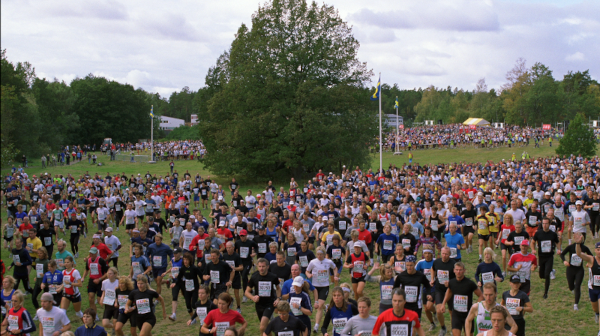
\includegraphics[height=0.4\textheight]{FIGURES/fig_36_1.png}
    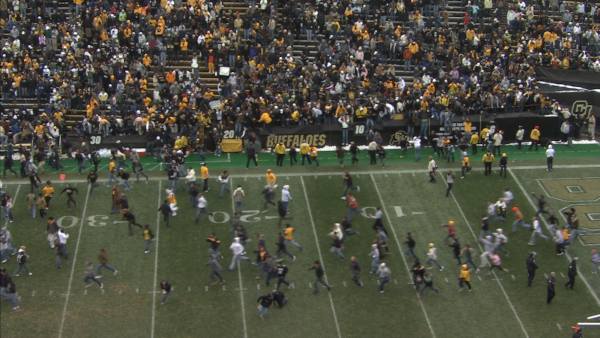
\includegraphics[height=0.4\textheight]{FIGURES/fig_36_2.png}
    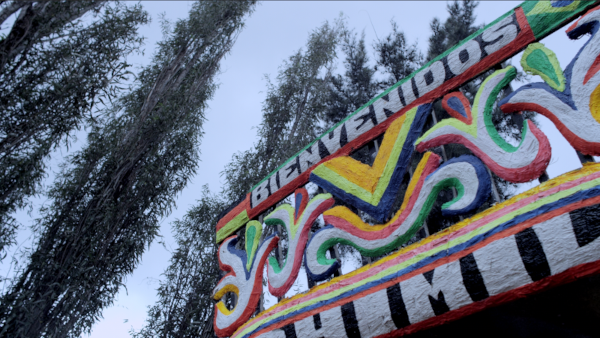
\includegraphics[height=0.4\textheight]{FIGURES/fig_36_3.png}
    \caption{Primeiro quadro das sequências HD1080 de maior destaque positivo em todos os experimentos, acima \textit{crowd\_run\_1080p50\_60f}, no meio \textit{rush\_field\_cuts\_1080p\_60f} e abaixo \textit{Netflix\_Boat\_1920x1080\_60fps\_8bit\_420\_60f}. Fonte: Elaborada pelo autor.}
    \label{fig:36}
\end{figure}
\end{landscape}
}

Desta forma, considerando tudo o que já foi abordado até o momento, é possível concluir que há sequências de vídeos em que as propostas de transcodificadores rápidos desenvolvidas apresentam resultados de redução de complexidade e impacto na eficiência de codificação dentro de valores desejáveis, como pode ser visto na Tabela \ref{tab:XXXVI}. Inclusive, as sequências com os resultados negativos nos mostram que há uma fragilidade na precisão do modelo implementado. Como apontado anteriormente, o uso da técnica de balanceamento de dados \textit{undersampling} aplica uma redução da capacidade de discernimento no limite entre decisões binárias. Desta forma, é preciso investigar e avaliar os melhores balanceamentos dos conjuntos de dados utilizados para treinamento e teste dos modelos, de forma a reduzir essa imprecisão entre particionar ou não particionar.

\afterpage{
\clearpage
\begin{landscape}
\begin{figure}
    \centering
    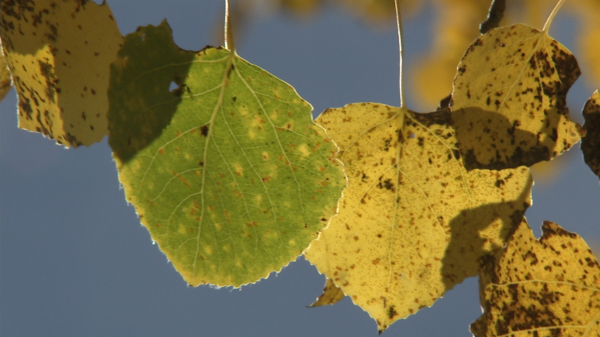
\includegraphics[height=0.4\textheight]{FIGURES/fig_37_1.png}
    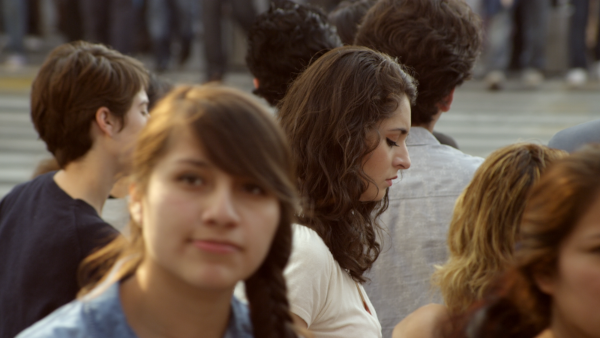
\includegraphics[height=0.4\textheight]{FIGURES/fig_37_2.png}
    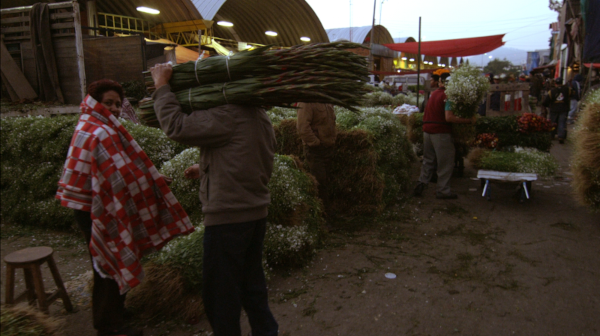
\includegraphics[height=0.4\textheight]{FIGURES/fig_37_3.png}
    \caption{Primeiro quadro das sequências HD1080 de maior destaque negativo em todos os experimentos, acima \textit{aspen\_1080p\_60f}, no meio \textit{Netflix\_Crosswalk\_1920x1080\_60fps\_8bit\_420\_60f} e abaixo \textit{Netflix\_FoodMarket\_1920x1080\_60fps\_8bit\_420\_60f}. Fonte: Elaborada pelo autor.}
    \label{fig:37}
\end{figure}
\end{landscape}
}


\chapter{Conclusão}
\label{cap:conclusao}

No decorrer desta tese, foram apresentadas a importância e a relevância do uso de codificadores de vídeo, em especial quando falamos em transmissões online de vídeos. Ao longo da história, diversos formatos de codificação de vídeo foram propostos, sendo que o de maior destaque no âmbito de \textit{streaming} é o H.264/AVC que ainda hoje em dia é largamente utilizado. Além deste formato, outros três formatos de codificação de vídeo são amplamente utilizados pela indústria de \textit{streaming} nos últimos anos: H.265/HEVC, VP9 e AV1. Recentemente foi publicado o formato H.266/VVC, atual estado da arte em termos de codificação de vídeo. Desses formatos, apenas o AV1 é livre de royalties e foi especialmente projetado para uso em serviços de transmissão pela internet e com alta capacidade de compressão de dados. Sendo assim, esta tese focou em soluções para o formato AV1.

Esta tese abordou a necessidade de realizar modificações nos vídeos codificados, mais especificamente através da transcodificação de vídeo, a fim de adequar os \textit{bitstreams} para as mais diversas condições do usuário. Há diversos estudos, sejam eles acadêmicos ou não, sobre a utilização de transcodificadores de vídeo. Os principais trabalhos acadêmicos visam a aceleração do processo, haja vista a complexidade de execução de um codificador de vídeo. As soluções existentes reduzem a complexidade de execução do transcodificador, buscando não comprometer significativamente a eficiência de codificação.

Esta tese apresentou  uma revisão sistemática da literatura e uma comparação entre trabalhos envolvendo transcodificação de vídeo desenvolvidos a partir do ano 2011 até o ano 2022. Muitas observações puderam ser feitas sobre esse levantamento bibliográfico, das quais destacamos as seguintes:

\begin{itemize}
    \item 70,69\% das transcodificações rápidas basearam as suas propostas de aceleração no reaproveitamento de informações referentes a estruturas de particionamento de blocos;
    
    \item A média de aceleração obtida (TS) com as propostas de transcodificador rápido foi de 50,74\%, havendo um desvio padrão de 19,23\% do tempo de execução em relação ao transcodificador original;

    \item O impacto de perda em eficiência de codificação tende a  4,11\%, podendo variar entre mais ou menos 2,46\%;

    \item O algoritmo de aprendizado de máquina mais utilizado foi a árvore de decisão C4.5/J48 (34,78\%).
\end{itemize}

Considerando o foco da tese em transcodificação rápida para o formato AV1, realizamos uma análise de complexidade do seu software de referência, o \textit{libaom}. Mais explicitamente, avaliamos o custo computacional de processar a árvore de particionamento de blocos do \textit{libaom} e o seu impacto na eficiência de codificação. A análise demonstrou que, dependendo da combinação de profundidades que se permite ao \textit{libaom} utilizar, podemos reduzir a complexidade de execução desde 12,88\% (a um custo de 0,39\% de BD-rate) até 76,66\% (a um custo de 103,56\% de BD-rate).

As análises também permitiram observar a distribuição das profundidades da árvore de particionamento de blocos. Por consequência, evidenciamos dois fatos que podem auxiliar na aceleração da transcodificação de vídeo usando o AV1 como destino: 1) identificar previamente a necessidade do \textit{libaom} de aprofundar o nível de profundidade tende a otimizar o funcionamento do \textit{libaom} e 2) evitar que o \textit{libaom} considere testar profundidades maiores que o necessário tende a reduzir a complexidade de execução do \textit{libaom}.


A hipótese explorada nesta tese de doutorado foi a de que ``\textit{a transcodificação de vídeo para o formato AV1 pode ser acelerada, com baixo impacto na eficiência de codificação, por meio do uso de uma metodologia comum para treinamento de modelos preditivos baseados em aprendizado de máquina, buscando inferir decisões na codificação a partir de dados extraídos tanto do bitstream original como do próprio processo de re-codificação}''. Assim, as explorações realizadas tiveram por objetivo \textbf{o desenvolvimento de um \textit{pipeline} de processamento que possibilitasse a criação ágil de transcodificadores rápidos} a partir de diversos formatos de codificação de vídeo e com o AV1 como formato de destino. 

Como resultado, além do \textit{pipeline} desenvolvido, a tese apresenta sete propostas de transcodificação rápida para o formato AV1. Duas delas são baseadas em análises estatísticas e heurísticas para predição das profundidades ou de orientação de blocos do AV1, enquanto cinco são baseadas em modelos preditivos gerados por algoritmos de aprendizado de máquina.

A proposta do transcodificador rápido de \textbf{H.265/HEVC para AV1} baseado em \textbf{heurísticas} se amparou na observação dos tamanhos de \textit{Coding Units} (CU) extraídos durante a decodificação do vídeo. Além disso, propomos a utilização de limitadores inferiores e superiores da árvore de particionamento do \textit{libaom}, tendo como base a profundidade da CU observada para uma determinada região do vídeo. Obtivemos, deste trabalho, 25 combinações de limitadores e, consequentemente, 25 resultados de transcodificação. Assim, foi possível chegar a uma aceleração máxima da transcodificação de 61,20\% (a um custo de 14,66\% de BD-rate) usando um limitador inferior e superior rígido, ou seja, aplicando, no AV1, a mesma profundidade de árvore que foi observada no H.265/HEVC. A solução permite funcionamento configurável, levando a uma \textbf{aceleração média de 40\% (a um custo de 5,02\% de BD-rate)}, ou 32\% (a um custo de 6,16\% de BD-rate), ou 20\% (a um custo de 3,90\% de BD-rate), ou 15,10\% (a um custo de 3,51\% de BD-rate), ou mesmo de 5\% (a um custo de 0,11\% de BD-rate).

A proposta do transcodificador rápido de \textbf{VP9 para AV1} baseado em \textbf{heurísticas} visou identificar a melhor orientação de blocos a ser aplicado na codificação AV1. Essa identificação se amparou  na correlação entre o nível de profundidade observado na decodificação do VP9, no nível de profundidade em processamento na codificação do AV1 e no nível de quantização utilizado. Através dessas três variáveis, aplicamos a orientação recomendada: bloco quadrático, blocos retangulares orientados à horizontal ou blocos retangulares orientados à vertical. Com essa proposta, foi possível obter uma \textbf{aceleração de 28,16\%, com uma perda de eficiência de codificação em 4,34\%}.

O uso de modelos preditivos gerados por \textbf{algoritmo de aprendizado de máquina} para acelerar a transcodificação de \textbf{VP9 para AV1} foi pensado para tomada de decisão nos três primeiros níveis de profundidade do AV1: 0 (do bloco quadrático de 128$\times$128 para 64$\times$64), 1 (do bloco quadrático de 64$\times$64 para 32$\times$32) e 2 (do bloco quadrático de 32$\times$32 para 16$\times$16). A fim de aumentar a precisão da resposta obtida pelo modelo, treinamos um modelo para cada profundidade e para cada nível de quantização utilizado (20, 32, 43 e 55). Portanto, a proposta do transcodificador rápido de VP9 para AV1 usou 12 modelos gerados por árvore de decisão a fim de obter indicativo de particionamento ou não do bloco atual em processamento. Essa solução é capaz de apresentar uma \textbf{aceleração média de 16,76\% a um custo 5,10\% de BD-rate}.

Com base na proposta desenvolvida de VP9 para AV1, usando modelos de aprendizado de máquina, desenvolvemos um \textit{pipeline} de processamento que automatizou as etapas de treinamento, teste e predição dos modelos. Esse \textit{pipeline} de processamento, considerando metodologias bem definidas, aplica automaticamente a transcodificação para obtenção das amostras para treinamento e teste e as transcodificações originais e rápidas, a fim de obter resultados comparativos de eficiência de codificação e redução de complexidade. Esse \textit{pipeline} facilita a adaptação do algoritmo em novas propostas, o que possibilitou o desenvolvimento de outras quatro soluções de transcodificadores para o AV1 de forma ágil, sendo que três delas são inéditas na literatura científica conhecida.

A proposta de transcodificador rápido de \textbf{H.264/AVC para AV1} baseado em \textbf{modelos de aprendizado de máquina}, desenvolvido através do \textit{pipeline} proposto, é capaz de atingir \textbf{reduções de complexidades de 25,05\%, a um custo de 5,58\% de BD-rate}. Destacamos que essa é uma solução inédita na literatura científica.

A proposta de transcodificador rápido de \textbf{VP8 para AV1} baseado em \textbf{modelos de aprendizado de máquina}, também desenvolvido através do \textit{pipeline} proposto, é capaz de atingir \textbf{reduções de complexidades média de 55,69\%, a um custo elevar o BD-rate em 12,85\%}. Destacamos que essa também é uma solução inédita na literatura científica.

A proposta de transcodificador rápido de \textbf{H.265/HEVC para AV1} baseado em \textbf{modelos de aprendizado de máquina}, também desenvolvido através do \textit{pipeline} proposto, obtém uma \textbf{aceleração de 28,36\%, a um custo de 6,74\% de BD-rate}.

A proposta de transcodificador rápido de \textbf{H.266/AVC para AV1} baseado em \textbf{modelos de aprendizado de máquina} é capaz de obter uma \textbf{aceleração de 12,05\% do tempo de codificação a um impacto de 1,67\% no BD-rate}, ao ser desenvolvido utilizando o \textit{pipeline} proposto. Destacamos que essa é uma solução inédita na literatura científica e a que melhor apresentou resultados gerais dentre todas as propostas de transcodificações rápidas desenvolvidas nesta tese.

Por fim, além das contribuições com soluções de transcodificadores rápidos para o formato AV1 já publicados e descritos um a um no Apêndice \ref{apx:C}, destacamos a \textbf{expansão do conhecimento acadêmico na área de transcodificação de vídeo}, em especial através do conteúdo disponibilizado no capítulo \ref{cap:3} desta tese e das soluções de transcodificadores rápidos para o formato AV1 ainda não publicados. Além disso, o desenvolvimento de um \textit{pipeline} de processamento tem potencial para auxiliar os pesquisadores e desenvolvedores a obter soluções rápidas para diversas combinações de formatos.



\bibliographystyle{abnt}
\bibliography{bibliografia} 

% Apêndices (Opcional) - Material produzido pelo autor
\apendices

\chapter{Relação das Sequências de Vídeos Utilizadas Na Tese}
\label{apx:A}

\afterpage{
\clearpage

\begin{landscape}
{\footnotesize
\begin{longtblr}[
    caption = {Relação das Sequências},
    entry   = none,
    note{1} = {bits = Profundidade de Bits},
    note{2} = {fps = Quadros por Unidade de Tempo},
    note{3} = {SI = Spatial Information},
    note{4} = {TI = Temporal Information}
]{
    colspec = {p{2cm}|p{5cm}|p{0.8cm}|p{2cm}|p{1cm}|p{1cm}|p{7cm}|p{2cm}},
    rowhead = 1,
    hlines,
    row{even} = {gray9}
}
\hline
\textbf{Classe} & \textbf{Sequência} & \textbf{bits\TblrNote{1}} & \textbf{fps\TblrNote{2}} & \textbf{\textit{SI\TblrNote{3}}} & \textbf{\textit{TI\TblrNote{4}}} & \textbf{Descrição} & \textbf{Presente no capítulo} \\
\SetCell[r=6]{c}Common Intermediate Format (CIF) & bqfree\_240p\_120f & 8 & 60000/1001 & 108,66 & 19,23 & pessoas saíndo de um shopping & \ref{cap:6.2.2} \\
 & bqhighway\_240p\_120f & 8 & 60000/1001 & 122,35 & 12,49 & vista aérea de uma sacada com uma ponte ao fundo & \ref{cap:6.2.1} \\
 & bqzoom\_240p\_120f & 8 & 30000/1001 & 84,74 & 10,3 & uma pessoa abanando enquanto a camera se abre & \ref{cap:6.2.2} \\
 & chairlift\_240p\_120f & 8 & 24000/1001 & 73,44 & 6,97 & vista externa de um teleférico com fundo de floresta & \ref{cap:6.2.2} \\
 & dirtbike\_240p\_120f & 8 & 24000/1001 & 62,27 & 4,86 & corrida de bicicleta em terreno acidentado & \ref{cap:6.2.1} \\
 & mozzoom\_240p\_120f & 8 & 30000/1001 & 79,75 & 28,69 & abertura de câmera do meio de uma árvore para um pedaço do parque & \ref{cap:6.2.2} \\
\SetCell[r=6]{c}Standard Definition (SD) & blue\_sky\_360p\_120f & 8 & 25/1 & 111,33 & 26,91 & camera mirando para o céu, com algumas árvores no canto, rotacionando & \ref{cap:6.2.1} \\
 & rain2\_hdr\_amazon\_360p & 10 & 24000/1001 & 41,62 & 2,54 & chuva em um telhado de vidro & \ref{cap:6.2.2} \\
 & red\_kayak\_360p\_120f & 8 & 30000/1001 & 63,56 & 28,71 & córrego marítmo agitado, às vezes aparece um remo e um bote & \ref{cap:6.2.2} \\
 & snow\_mnt\_640x360\_120f & 8 & 30000/1001 & 123,76 & 2,02 & cenário de montanha com uma núvem se movimentando & \ref{cap:6.2.2} \\
 & tacomanarrows360p\_120f & 8 & 30/1 & 67,45 & 1,8 & pessoas numa reunião de escritório & \ref{cap:6.2.2} \\
 & water\_hdr\_amazon\_360p & 10 & 24000/1001 & 26,57 & 1,49 & cenário de mar num por do sol & \ref{cap:6.2.1} \\
\SetCell[r=2]{c}HD720 & boat\_hdr\_amazon\_720p & 10 & 24000/1001 & 47,12 & 7,78 & bote balançando em um cais & \ref{cap:7.5} \\
 & dark720p\_120f & 8 & 30/1 & 40,15 & 5,13 & pessoa ajustando câmera em um escritório & \ref{cap:6.2.2} e \ref{cap:7.5} \\
\SetCell[r=14]{c}High Definition 720 (HD720) & FourPeople\_1280x720\_60 & 8 & 60/1 & 69,1 & 4,08 & quatro pessoas em uma reunião de escritório & \ref{cap:7.5} \\
 & FourPeople\_1280x720\_60\_120f & 8 & 60/1 & 69,12 & 3,98 & quatro pessoas em uma reunião de escritório & \ref{cap:7.5} \\
 & gipsrestat720p\_120f & 8 & 50/1 & 76,74 & 2,89 & duas pessoas conversando em uma sala cheia de roupas & \ref{cap:7.5} \\
 & Johnny\_1280x720\_60 & 8 & 60/1 & 55,15 & 3,36 & reporter falando com a câmera & \ref{cap:7.5} \\
 & Johnny\_1280x720\_60\_120f & 8 & 60/1 & 55,13 & 3,29 & reporter falando com a câmera & \ref{cap:6.2.2} e \ref{cap:7.5} \\
 & KristenAndSara\_1280x720\_60 & 8 & 60/1 & 73,8 & 3,07 & duas repórteres conversando & \ref{cap:7.5} \\
 & KristenAndSara\_1280x720 \_60\_120f & 8 & 60/1 & 73,78 & 3,03 & duas repórteres conversando & \ref{cap:7.5} \\
 & Netflix\_DinnerScene\_1280x720 \_60fps\_8bit\_420\_120f & 8 & 60/1 & 16,07 & 2,31 & camera adentrando uma sala de jantar escura & \ref{cap:6.2.1} e \ref{cap:7.5} \\
 & Netflix\_DrivingPOV\_1280x720 \_60fps\_8bit\_420\_120f & 8 & 60/1 & 77,59 & 12,32 & câmera andando por uma alameda e alguns carros & \ref{cap:6.2.2} e \ref{cap:7.5} \\
 & Netflix\_FoodMarket2\_1280x720 \_60fps\_8bit\_420\_120f & 8 & 60/1 & 56,83 & 24,89 & cenário de uma feira de frutas, com câmera se deslocando junto com um carrinho & \ref{cap:6.2.1} e \ref{cap:7.5} \\
 & Netflix\_RollerCoaster\_1280x720 \_60fps\_8bit\_420\_120f & 8 & 60/1 & 49,38 & 18,53 & câmera de dentro de um carrinho de montanha russa durante uma curva & \ref{cap:6.2.2} e \ref{cap:7.5} \\
 & Netflix\_Tango\_1280x720 \_60fps\_8bit\_420\_120f & 8 & 60/1 & 45,42 & 15,43 & pessoas dançando em uma roda de tango & \ref{cap:7.5} \\
 & rain\_hdr\_amazon\_720p & 10 & 24000/1001 & 53,6 & 3,67 & pessoa caminhando em um cenário chuvoso & \ref{cap:7.5} \\
 & vidyo1\_720p\_60fps\_120f & 8 & 60/1 & 53,29 & 4,12 & três pessoas conversando em um escritório & \ref{cap:7.5} \\
\SetCell[r=5]{c}High Definition 720p (HD720) & Vidyo1\_1280x720\_60 & 8 & 60/1 & 53,28 & 4,18 & três pessoas conversando em um escritório & \ref{cap:7.5} \\
 & vidyo3\_720p\_60fps\_120f & 8 & 60/1 & 60,38 & 7,91 & pessoa dando aula & \ref{cap:7.5} \\
 & Vidyo3\_1280x720\_60 & 8 & 60/1 & 60,56 & 8 & pessoa dando aula & \ref{cap:7.5} \\
 & vidyo4\_720p\_60fps\_120f & 8 & 60/1 & 51,68 & 7,43 & pessoa falando com a câmera & \ref{cap:7.5} \\
 & Vidyo4\_1280x720\_60 & 8 & 60/1 & 51,66 & 7,57 & pessoa falando com a câmera & \ref{cap:7.5} \\
\SetCell[r=9]{c}High Definition 1080p (HD1080) & aspen\_1080p\_60f & 8 & 30000/1001 & 30,4 & 10,08 & folhas de árvore balançando & \ref{cap:6.1.1} e \ref{cap:7.5} \\
 & BasketballDrive\_1920x1080\_50 & 8 & 50/1 & 54,96 & 19,95 & partida de basquete & \ref{cap:5.2} e \ref{cap:6.1.2} e \ref{cap:7.3} \\
 & BQTerrace\_1920x1080\_60 & 8 & 60/1 & 105,06 & 14,21 & área externa de um restaurante com pessoas se alimentando & \ref{cap:5.2} e \ref{cap:6.1.1} e \ref{cap:7.3} \\
 & Cactus\_1920x1080\_50 & 8 & 50/1 & 63,52 & 12,87 & cenário com diversos brinquedos se movendo ao mesmo tempo & \ref{cap:5.2} e \ref{cap:6.1.1} e \ref{cap:7.3} \\
 & crowd\_run\_1080p50\_60f & 8 & 50/1 & 93,04 & 21,14 & muitas pessoas correndo em um campo & \ref{cap:5.1} e \ref{cap:6.2.2} e \ref{cap:7.5} \\
 & CrowdRun\_1920x1080\_25 & 8 & 24/1 & 91,42 & 28,35 & muitas pessoas correndo em um campo & \ref{cap:5.2} e \ref{cap:6.1.2} e \ref{cap:7.3} \\
 & ducks\_take\_off\_1080p50\_60f & 8 & 50/1 & 71,27 & 10,57 & patos nadando em um lago & \ref{cap:7.5} \\
 & FountainSky\_1920x1080p30 \_130f & 8 & 30000/1001 & 135,72 & 13,84 & foco em um chafariz calmo com pessoas caminhando ao fundo & \ref{cap:5.2} e \ref{cap:7.3} \\
 & guitar\_hdr\_amazon\_1080p & 10 & 24000/1001 & 19,68 & 6,61 & senhor tocando violão em um fundo desfocado & \ref{cap:5.1} e \ref{cap:6.2.1} e \ref{cap:7.5} \\
\SetCell[r=12]{c}High Definition 1080p (HD1080) & Kimono1\_1920x1080\_24 & 8 & 24/1 & 23,12 & 13,48 & mulher de kimono caminhando com árvores ao fundo & \ref{cap:5.2} e \ref{cap:7.3} \\
 & Netflix\_Aerial\_1920x1080 \_60fps\_8bit\_420\_60f & 8 & 60/1 & 46,83 & 8,69 & pessoas controlando o início do vôo de um drone & \ref{cap:6.1.1} e \ref{cap:7.5} \\
 & Netflix\_Boat\_1920x1080 \_60fps\_8bit\_420\_60f & 8 & 60/1 & 82,07 & 16,82 & letreiro com fundo de céu aberto se deslocando & \ref{cap:6.1.1} e \ref{cap:7.5} \\
 & Netflix\_Crosswalk\_1920x1080 \_60fps\_8bit\_420\_60f & 8 & 60/1 & 19,8 & 12,87 & pessoas em um cruzamento & \ref{cap:5.1} e \ref{cap:6.2.2} e \ref{cap:7.5} \\
 & Netflix\_FoodMarket\_1920x1080 \_60fps\_8bit\_420\_60f & 8 & 60/1 & 34,31 & 14,42 & câmera mostrando uma feira de flores & \ref{cap:7.5} \\
 & Netflix\_PierSeaside\_1920x1080 \_60fps\_8bit\_420\_60f & 8 & 60/1 & 55,35 & 12,49 & câmera mostrando um pier & \ref{cap:7.5} \\
 & Netflix\_SquareAndTimelapse\_1920x1080 \_60fps\_8bit\_420\_60f & 8 & 60/1 & 57,92 & 18,71 & muitas pessoas olhando um festival chinês & \ref{cap:5.1} e \ref{cap:7.5} \\
 & Netflix\_TunnelFlag\_1920x1080 \_60fps\_8bit\_420\_60f & 8 & 60/1 & 88,8 & 51,51 & veículo se deslocando em um túnel de vidro & \ref{cap:5.1} e \ref{cap:6.1.1} e \ref{cap:6.2.1} e \ref{cap:7.5} \\
 & old\_town\_cross\_1080p50\_60f & 8 & 50/1 & 52,51 & 9,55 & vista aérea da cidade de Estocolmo & \ref{cap:7.5} \\
 & pan\_hdr\_amazon\_1080p & 10 & 24000/1 & 33,1 & 10,02 & deslocamento de câmera em um cais a noite & \ref{cap:7.5} \\
 & park\_joy\_1080p50\_60f & 8 & 50/1 & 89,5 & 30,16 & pessoas correndo ao fundo próximos a um lago, árvores passando em primeiro plano & \ref{cap:6.2.2} e \ref{cap:7.5} \\
 & ParkScene\_1920x1080\_24 & 8 & 24/1 & 49,67 & 11,29 & cenário de parque com bicicletas passando & \ref{cap:5.2} e \ref{cap:6.1.1} e \ref{cap:7.3} \\
\SetCell[r=12]{c}High Definition 1080p (HD1080) & pedestrian\_area\_1080p25\_60f & 8 & 25/1 & 31,47 & 17,85 & pessoas andando em uma rua & \ref{cap:7.5} \\
 & rush\_field\_cuts\_1080p\_60f & 8 & 30000/1001 & 81,15 & 11,37 & pessoas invadindo um campo de NFL & \ref{cap:7.5} \\
 & rush\_hour\_1080p25\_60f & 8 & 25/1 & 22,7 & 10,11 & câmera no meio de uma rua de mão dupla, mostrando um engarrafamento & \ref{cap:6.1.2} e \ref{cap:7.5} \\
 & seaplane\_hdr\_amazon\_1080p & 10 & 24000/1001 & 44,99 & 14,15 & hidroavião estacionando no cais & \ref{cap:6.1.2} e \ref{cap:6.2.2} e \ref{cap:7.5} \\
 & Skater227\_1920x1080\_30fps & 10 & 30/1 & 13,52 & 16,37 & foco no rosto de uma menina aprendendo a andar de skate & \ref{cap:5.2} e \ref{cap:7.3} \\
 & station2\_1080p25\_60f & 8 & 25/1 & 29,18 & 10,91 & abertura de câmera de um terminal ferroviário & \ref{cap:7.5} \\
 & Tennis\_1920x1080\_24 & 8 & 24/1 & 35,12 & 27,79 & pessoas jogando tênis & \ref{cap:5.2} e \ref{cap:6.1.1} e \ref{cap:7.3} \\
 & TimeLapseStreet\_1920x1080 p30\_130f & 8 & 30/1 & 58,48 & 5,74 & fade-in de uma rua com carros estacionados & \ref{cap:5.2} e \ref{cap:7.3} \\
 & Wheat\_1920x1080 & 8 & 30000/1001 & 48,15 & 7,35 & cena fixa de uma paisagem de outono com folhagens levemente se movendo ao vento & \ref{cap:5.2} e \ref{cap:7.3} \\
 & WorldCup\_1920x1080\_30p & 8 & 30/1 & 50,26 & 19,92 & pessoas de costas comemorando & \ref{cap:5.2} e \ref{cap:7.3} \\
 & WorldCup\_far\_1920x1080\_30p & 8 & 30/1 & 67,36 & 23,73 & várias pessoas sobre um chafariz comemorando na frente de um prédio histórico com fumaças & \ref{cap:5.2} e \ref{cap:7.3} \\
 & WorldCupFarSky\_1920x1080 \_30p & 8 & 30/1 & 65,67 & 12,18 & várias pessoas sobre um chafariz comemorando ao lado de um telão de comercial & \ref{cap:5.2} e \ref{cap:7.3} \\
\SetCell[r=4]{c}HD1080 com Screen Content Coding (HD1080 + SCC) & DOTA2\_60f\_420 & 8 & 60/1 & 63,12 & 6,6 & animação, partida calma de DOTA, há troca de cena no final & \ref{cap:6.2.2} \\
 & MINECRAFT\_60f\_420 & 8 & 60/1 & 71,43 & 27,01 & animação, jogador se deslocando em um cenário de minecraft & \ref{cap:6.2.2} \\
 & STARCRAFT\_60f\_420 & 8 & 60/1 & 83,9 & 2,82 & animação, partida calma de Starcraft & \ref{cap:6.2.2} \\
 & wikipedia\_420 & 8 & 30/1 & 147,1 & 35,42 & tela com Google Chrome aberta, usuário movimenta página da Wikipédia muito rápido & \ref{cap:6.2.2} \\
\SetCell[r=7]{c}Ultra High Definition 4K (UHD4K) & Netflix\_BarScene\_4096x2160 \_60fps\_10bit\_420\_60f & 10 & 60/1 & 12,17 & 3,88 & garota jogando curling de mesa, foco acompanha a bola & \ref{cap:7.5} \\
 & Netflix\_BoxingPractice\_ 4096x2160\_60fps\_10bit\_420\_60f & 10 & 60/1 & 34,99 & 16,68 & pessoas particamento atividades em uma academia de boxe & \ref{cap:7.5} \\
 & Netflix\_Dancers\_4096x2160 \_60fps\_10bit\_420\_60f & 10 & 60/1 & 10,12 & 5,81 & pessoas se aproximando em um fundo preto & \ref{cap:7.5} \\
 & Netflix\_Narrator\_4096x2160 \_60fps\_10bit\_420\_60f & 10 & 60/1 & 19,07 & 5,85 & jornalista apresentando uma matéria na rua & \ref{cap:7.5} \\
 & Netflix\_RitualDance\_4096x2160 \_60fps\_10bit\_420\_60f & 10 & 60/1 & 21,8 & 14,96 & pessoas assistindo um festival de dança & \ref{cap:7.5} \\
 & Netflix\_ToddlerFountain\_4096 x2160\_60fps\_10bit\_420\_60f & 10 & 60/1 & 44,51 & 27,07 & criança corre por uma parquinho de geisers artificiais & \ref{cap:7.5} \\
 & Netflix\_WindAndNature\_4096 x2160\_60fps\_10bit\_420\_60f & 10 & 60/1 & 36,91 & 7,07 & câmera focada em um parque de anemômetros funcionando & \ref{cap:7.5} \\
\SetCell[r=1]{c}UHD4K & street\_hdr\_amazon\_2160p & 10 & 24000/1001 & 27,88 & 4,52 & caminhão passando ao fundo em uma alameda arborizada com vento & \ref{cap:7.5} \\
\hline
\end{longtblr}
}
\end{landscape}
}

\chapter{Cálculo das combinações de árvores do AV1}
\label{apx:B}

Neste apêndice encontra-se o código utilizado para obter o número de arranjos de árvores de particionamento disponíveis para uso pelo software de referência do AV1, considerando alguns parâmetros conhecidos. Este código foi utilizado no capítulo \ref{cap:5}

\begin{minted}[linenos]{python}
#Definindo os particionamentos permitidos para cada profundidade
allow_on_depth_128 = ['none', 'horz', 'vert', 'horz_a', 'horz_b', 
                      'vert_a', 'vert_b', 'split']
allow_on_depth_64  = ['none', 'horz', 'vert', 'horz_a', 'horz_b', 
                      'vert_a', 'vert_b', 'horz_4', 'vert_4', 'split']
allow_on_depth_32  = ['none', 'horz', 'vert', 'horz_a', 'horz_b', 
                      'vert_a', 'vert_b', 'horz_4', 'vert_4', 'split']
allow_on_depth_16  = ['none', 'horz', 'vert', 'horz_a', 'horz_b', 
                      'vert_a', 'vert_b', 'horz_4', 'vert_4', 'split']
allow_on_depth_8   = ['none', 'horz', 'vert', 'split']
allow_on_depth_4   = ['none']
 
#unificando todas as profundidades
ptypes_allowed = [allow_on_depth_128, allow_on_depth_64, 
                  allow_on_depth_32, allow_on_depth_16, 
                  allow_on_depth_8, allow_on_depth_4]
 
#definindo os particionamentos proibidos nas 3 combinações abaixo
rule_rect = ['horz', 'vert', 'horz_a', 'horz_b', 'vert_a', 'vert_b', 
             'horz_4', 'vert_4']
rule_ab   = ['horz_a', 'horz_b', 'vert_a', 'vert_b']
rule_1TO4 = ['horz_4', 'vert_4']
 
#dict que traduz o tamanho do bloco em profundidade
dpt_translator = {128:0, 64:1, 32:2, 16:3, 8:4, 4:5}

#função que calcula o máximo de combinações de árvores possível
def original_tree(Node, depth):
 i = 0
 for ptype in Node[depth]:
   if ptype == 'split':
     i += original_tree(Node, depth + 1)
     i += original_tree(Node, depth + 1)
     i += original_tree(Node, depth + 1)
     i += original_tree(Node, depth + 1)
   else:
       i += 1
 return i
 
#função que calcula o máximo de combinações de árvores possível,
#excluíndo os ptypes proibidos
def limit_ptype_tree(Node, depth, forbid):
 i = 0
 for ptype in Node[depth]:
   if ptype == 'split':
     i += limit_ptype_tree(Node, depth + 1, forbid)
     i += limit_ptype_tree(Node, depth + 1, forbid)
     i += limit_ptype_tree(Node, depth + 1, forbid)
     i += limit_ptype_tree(Node, depth + 1, forbid)
   elif not (ptype in forbid):
     i += 1
 return i
 
#função que calcula o máximo de combinações de árvores possível, 
#evitando as profundidades proibidas
def limit_tree_depth(Node, depth, max, min):
 i = 0
 if depth < max:
   i += limit_tree_depth(Node, depth + 1, max, min)
   i += limit_tree_depth(Node, depth + 1, max, min)
   i += limit_tree_depth(Node, depth + 1, max, min)
   i += limit_tree_depth(Node, depth + 1, max, min)
 elif depth > min:
   return i
 else:
   for ptype in Node[depth]:
     if ptype == 'split':
       i += limit_tree_depth(Node, depth + 1, max, min)
       i += limit_tree_depth(Node, depth + 1, max, min)
       i += limit_tree_depth(Node, depth + 1, max, min)
       i += limit_tree_depth(Node, depth + 1, max, min)
     else:
         i += 1
 return i

#Saída de todos os casos
print("original", original_tree(ptypes_allowed, 0))
 
print("rect    ", limit_ptype_tree(ptypes_allowed, 0, rule_01))
print("ab      ", limit_ptype_tree(ptypes_allowed, 0, rule_02))
print("1TO4    ", limit_ptype_tree(ptypes_allowed, 0, rule_03))
 
print("128-64  ", limit_tree_depth(ptypes_allowed, 
                                   0,
                                   dpt_translator[128], 
                                   dpt_translator[64]))
print("128-32  ", limit_tree_depth(ptypes_allowed,
                                   0, 
                                   dpt_translator[128], 
                                   dpt_translator[32]))
print("128-16  ", limit_tree_depth(ptypes_allowed, 
                                   0, 
                                   dpt_translator[128], 
                                   dpt_translator[16]))
print("128-8   ", limit_tree_depth(ptypes_allowed, 
                                   0, 
                                   dpt_translator[128], 
                                   dpt_translator[8]))
 
print("64-32   ", limit_tree_depth(ptypes_allowed, 
                                   0,  
                                   dpt_translator[64], 
                                   dpt_translator[32]))
print("64-16   ", limit_tree_depth(ptypes_allowed, 
                                   0,  
                                   dpt_translator[64], 
                                   dpt_translator[16]))
print("64-8    ", limit_tree_depth(ptypes_allowed, 
                                   0,  
                                   dpt_translator[64], 
                                   dpt_translator[8]))
print("64-4    ", limit_tree_depth(ptypes_allowed, 
                                   0,  
                                   dpt_translator[64], 
                                   dpt_translator[4]))
 
print("32-16   ", limit_tree_depth(ptypes_allowed, 
                                   0,  
                                   dpt_translator[32], 
                                   dpt_translator[16]))
print("32-8    ", limit_tree_depth(ptypes_allowed, 
                                   0,  
                                   dpt_translator[32], 
                                   dpt_translator[8]))
print("32-4    ", limit_tree_depth(ptypes_allowed, 
                                   0,  
                                   dpt_translator[32], 
                                   dpt_translator[4]))
 
print("16-8    ", limit_tree_depth(ptypes_allowed, 
                                   0,  
                                   dpt_translator[16], 
                                   dpt_translator[8]))
print("16-4    ", limit_tree_depth(ptypes_allowed, 
                                   0,  
                                   dpt_translator[16], 
                                   dpt_translator[4]))
 
print("8-4     ", limit_tree_depth(ptypes_allowed, 
                                   0,  
                                   dpt_translator[8], 
                                   dpt_translator[4]))

\end{minted}
\chapter{Publicações e Apresentações Realizadas Durante o Doutorado}
\label{apx:C}

Durante o desenvolvimento desta tese, algumas publicações foram realizadas no contexto da própria tese ou em colaboração com colegas pesquisadores. Segue-se abaixo as indicações dos trabalhos, divididos em tópicos:

\begin{enumerate}
     \item \textbf{Artigos Publicados em Revistas Científicas}:
    \begin{enumerate}
        \item ``\textit{Complexity-scalable HEVC-to-AV1 video transcoding based on partition inheritance}'', publicada na revista Journal of Real-Time Image Processing \cite{bib:borges2_2021};

        \item ``\textit{AV1 and VVC Video Codecs: Overview on Complexity Reduction and Hardware Design}'', co-autor do trabalho publicado na revista IEEE Open Journal of Circuits and Systems.
    \end{enumerate}
    
    \item \textbf{Artigos Publicados em Conferências}:
    \begin{enumerate}
        \item ``\textit{Fast VP9-to-AV1 Transcoding based on Block Partitioning Inheritance}'', publicado no 28th European Signal Processing Conference \cite{bib:borges_2021};

        \item ``\textit{Identifying Energy-Saving Opportunities for AV1 Video Coding in Streaming Services}'', co-autor do trabalho publicado no 28th European Signal Processing Conference \cite{bib:camargo_2022};

        \item ``\textit{H.264-to-AV1 Video Transcoding Acceleration Based on Lightweight Machine Learning}'', a ser publicado na IEEE International Symposium on Circuits \& Systems \cite{bib:borges_iscas_2023}.
    \end{enumerate}
    
    \item \textbf{Resumos Expandidos}:
    \begin{enumerate}
        \item ``\textit{Análise do Particionamento de Superblocos do Formato de Vídeo AV1}'', publicado no XXII Encontro de Pós-Graduação \cite{bib:enpos_2020};

        \item ``\textit{Análise de Complexidade Escalável para a Transcodificação de Vídeo de HEVC para AV1}'', publicado no XXIII Encontro de Pós-Graduação \cite{bib:enpos_2021};

        \item ``\textit{Transcodificação de Vídeo Acelerada de VP9 para AV1 Usando Árvore de Decisão e Estruturas de Particionamento}'', publicado no XXIV Encontro de Pós-Graduação \cite{bib:enpos_2022}.
    \end{enumerate}

    \item \textbf{Apresentação de Pôsteres}:
    \begin{enumerate}
        \item ``\textit{Complexity-Scalable HEVC-to-AV1 Video Transcoding Based on Partition Inheritance}'', apresentado no 4th IEEE SPS/CASS Seasonal School on Digital Processing of Visual Signals and Application \cite{bib:dpvsa_2020}; 

        \item ``\textit{Fast VP9-to-AV1 Transcoding Based on Block Partitioning Inheritance}'', apresentado no 5th IEEE SPS/CASS Seasonal School on Digital Processing of Visual Signals and Application \cite{bib:dpvsa_2021};

        \item ``\textit{Decision Trees for Accelerating H.264/AVC-to-AV1 Video Transcoding}'', apresentado no 6th IEEE SPS/CASS Seasonal School on Digital Processing of Visual Signals and Application \cite{bib:dpvsa_2022};

        \item ``\textit{Energy-Saving Opportunities for AV1 Video Coding in Streaming Services}'', apresentado em co-autoria no 6th IEEE SPS/CASS Seasonal School on Digital Processing of Visual Signals and Application \cite{bib:dpvsa_2022_carol}.
    \end{enumerate}

\end{enumerate}


\end{document}
